%\documentclass[a4paper,11pt]{book}
\documentclass[b5paper,11pt]{book}
%\documentclass[a4paper,12pt]{book}
%\usepackage{setspace}
%\doublespacing
\usepackage[paperwidth=17cm, paperheight=24cm, top=30mm, bottom=30mm, outer=30mm, inner=20mm]{geometry}
\usepackage{color}
\usepackage[cmyk]{xcolor}
%\usepackage{showframe}
%\usepackage{layout}

\usepackage{feynmp}
\usepackage[colorlinks,linkcolor=black,citecolor=black,filecolor=black,urlcolor=black,plainpages=false,unicode=false,pdfencoding=auto]{hyperref}
\usepackage{ifthen}
\usepackage{datetime}
\usepackage{graphicx}
\usepackage{caption}
\usepackage{subcaption}
\usepackage{wrapfig}
\usepackage{upgreek}
\usepackage{bbold}
\usepackage{amsmath}
\usepackage{amssymb}
\usepackage{mathtools}
\usepackage{bm}
\usepackage[switch,running]{lineno}
\usepackage{cite}
\usepackage{mciteplus}
\usepackage{tikz}
\usetikzlibrary{arrows,shapes,backgrounds}
\usepackage{fancyhdr}
\pagestyle{fancy}
\setlength{\headheight}{15.2pt}
%\setlength{\headheight}{16.5pt}
\rhead[\nouppercase\leftmark]{\thepage}
\lhead[\thepage]{\nouppercase\rightmark}
\cfoot{}
\usepackage[labelfont=bf,textfont=it]{caption}
\usepackage{enumitem}
\setlist[description]{leftmargin=0pt,style=nextline}

\usepackage[ttscale=.875]{libertine}
%\usepackage[]{fontspec}
%\usepackage{unicode-math}
%\setmainfont{Linux Libertine O}
\setmonofont[Scale=MatchLowercase]{DejaVuSansMono.ttf}
%\setmathfont{latinmodern-math.otf}
%\setmathfont[range=\mathit/{latin,Latin,num,Greek,greek}]{LinLibertine_I.otf}
%\setmathfont[range=\mathup/{latin,Latin,num,Greek,greek}]{LinLibertine_R.otf}
%\setmathfont[range=\mathbfup/{latin,Latin,num,Greek,greek}]{LinLibertine_RB.otf}
%\setmathfont[range={"221E}]{LinLibertine_R.otf}% "0221E = \infty

\usepackage{rotating}
\usepackage{xargs}

\newboolean{articletitles}
\setboolean{articletitles}{false}

\DeclareGraphicsRule{*}{eps}{*}{}

\allowdisplaybreaks

\renewcommand{\bibname}{References}

\newcommand{\cern}{\textsc{Cern}}
\newcommand{\atlas}{\textsc{Atlas}}
\newcommand{\velo}{\textsc{Velo}}
\newcommand{\ecal}{\textsc{ECal}}
\newcommand{\hcal}{\textsc{HCal}}
\newcommand{\rich}{\textsc{Rich}}

\newcommand{\splot}[1][]{\textsubscript{\textit{s}}$\mathcal{P}$\textit{lot#1}}
\newcommand{\sweight}[1][]{sWeight#1}

\newcommand{\mss}[1]{{\scriptstyle #1}}
\newcommand{\ud}{\mathrm{d}}
\renewcommand{\vec}{\bm}

\newcommand{\unitsp}{\,}
\newcommand{\texteq}{\unitsp=\unitsp}
\renewcommand{\textneq}{\unitsp≠\unitsp}
\newcommand{\textlt}{\unitsp<\unitsp}
\newcommand{\textgt}{\unitsp>\unitsp}
\renewcommand{\textle}{\unitsp≤\unitsp}
\renewcommand{\textge}{\unitsp≥\unitsp}
\renewcommand{\textll}{\unitsp≪\unitsp}
\renewcommand{\textequiv}{\unitsp≡\unitsp}
\renewcommand{\textapprox}{\unitsp≈\unitsp}
\newcommand{\textplus}{\unitsp+\unitsp}
\renewcommand{\textminus}{\unitsp--\unitsp}
\renewcommand{\textpm}{\unitsp±\unitsp}
\renewcommand{\textmp}{\unitsp∓\unitsp}
\newcommand{\textto}{\unitsp→\unitsp}
\newcommand{\tp}{+}
\newcommand{\tm}{--}
\newcommand{\tpm}{±}
\newcommand{\tmp}{∓}
\renewcommand{\texttimes}{\unitsp×\unitsp}
\renewcommand{\textcdot}{\unitsp·\unitsp}
\newcommand{\ttimes}{×}
\renewcommand{\textin}{\unitsp∈\unitsp}
\newcommand{\tpi}{π}
\newcommand{\ctm}{\multicolumn{1}{c}{--}}
\newcommand{\tenpow}[1]{10\textsuperscript{#1}}
\newcommand{\tenpowmult}[1]{$\,\cdot\,$10\textsuperscript{#1}}
\newcommand{\micron}{μm}
\newcommand{\invfb}{fb\textsuperscript{--1}}
\newcommand{\invps}{ps\textsuperscript{--1}}
\newcommand{\eV}{eV/$c$\textsuperscript{2}}
\newcommand{\MeV}{MeV/$c$\textsuperscript{2}}
\newcommand{\GeV}{GeV/$c$\textsuperscript{2}}
\newcommand{\eVc}{eV/$c$}
\newcommand{\MeVc}{MeV/$c$}
\newcommand{\GeVc}{GeV/$c$}
\newcommand{\pT}{p_\mathrm{T}}

\newcommand{\Wpm}[1][±]{\text{W}^{\text{#1}}}
\newcommand{\Wp}{\Wpm[+]}
\newcommand{\Wm}{\Wpm[--]}
\newcommand{\Zz}{\text{Z}^{\text{0}}}
\newcommand{\lepe}[1][]{\text{e}^\text{#1}}
\newcommand{\lmu}[1][]{\text{μ}^\text{#1}}
\newcommand{\ltau}[1][]{\text{τ}^\text{#1}}
\newcommand{\nul}[1][]{\text{ν}_\text{#1}}
\newcommand{\nulbar}[1][]{\kern 0.04em \overline{\kern -0.04em \nul[#1] \kern -0.25em} \kern 0.25em}
\newcommand{\nue}{\nul[e]}
\newcommand{\numu}{\nul[μ]}
\newcommand{\nutau}{\nul[τ]}
\newcommand{\nuebar}{\nulbar[e]}
\newcommand{\numubar}{\nulbar[μ]}
\newcommand{\nutaubar}{\nulbar[τ]}
\newcommand{\mup}{\lmu[+]}
\newcommand{\mum}{\lmu[--]}
\newcommand{\qbar}[1][b]{\kern 0.06em \overline{\kern -0.06em \text{#1} \kern -0.04em} \kern 0.04em}
\newcommand{\ccs}{\text{c}\qbar[c]\text{s}}
\newcommand{\btoccs}{\text{b}\to\ccs}
\newcommand{\bbbar}{\text{b}\qbar[b]}
\newcommand{\pimes}[1][]{\text{π}^\text{#1}}
\newcommand{\phimes}{\text{ϕ}\text{(1020)}}
\newcommand{\phimesalt}{\text{ϕ}}
\newcommand{\fzero}{\text{f}_\text{0}\text{(980)}}
\newcommand{\ftwop}{\text{f}_\text{2}^{\,\prime}\text{(1525)}}
\newcommand{\Jpsi}{\text{J}/\text{ψ}}
\newcommand{\psitwoS}{\text{ψ(2S)}}
\newcommand{\upsS}[1][1]{\text{Y(#1S)}}
\newcommand{\kaon}[1][0]{\text{K}^\text{#1}}
\newcommand{\Kp}{\kaon[+]}
\newcommand{\Km}{\kaon[--]}
\newcommand{\KS}{\kaon_\text{S}}
\newcommand{\Kst}{\text{K}^{\ast \kern 0.01em \text{0}}}
\newcommand{\Kstbar}{\kern 0.06em \overline{\kern -0.06em \Kst \kern -0.44em} \kern 0.44em}
\newcommand{\Dmes}[1][0]{\text{D}^\text{#1}}
\newcommand{\Dsmes}[1][0]{\text{D}_\text{s}^\text{#1}}
\newcommand{\Bd}{\text{B}^\text{0}}
\newcommand{\Bdbar}{\kern 0.06em \overline{\kern -0.06em \Bd \kern -0.32em} \kern 0.32em}
\newcommand{\Bs}{\text{B}_\text{s}^\text{0}}
\newcommand{\Bsbar}{\kern 0.06em \overline{\kern -0.06em \Bs \kern -0.32em} \kern 0.32em}
\newcommand{\Bc}{\text{B}_\text{c}^\text{+}}
\newcommand{\prot}{\text{p}}
\newcommand{\Lb}{\text{Λ}_\text{b}^\text{0}}
\newcommand{\BH}{\text{B}_\text{H}}
\newcommand{\BL}{\text{B}_\text{L}}
\newcommand{\BE}{\text{B}_\text{E}}
\newcommand{\BO}{\text{B}_\text{O}}
\newcommand{\Bsst}{|\Bs\rangle}
\newcommand{\Bsbarst}{|\Bsbar\rangle}
\newcommand{\BLst}{|\BL\rangle}
\newcommand{\BHst}{|\BH\rangle}
\newcommand{\fp}{\text{f}^{\,\prime}}
\newcommand{\fst}{|\text{f}\rangle}
\newcommand{\fbarst}{|\overline{\text{f}}\rangle}
\newcommand{\BsBsbar}{$\Bs$--$\Bsbar$}
\newcommand{\mumu}{\mup\mum}
\newcommand{\hh}{\text{h}^\text{+}\text{h}^\text{--}}
\newcommand{\KK}{\Kp\Km}
\newcommand{\pipi}{\pimes[+]\pimes[--]}
\newcommand{\Kpi}{\Kp\pimes[--]}
\newcommand{\mumuhh}{\mumu\,\hh}
\newcommand{\mumuKK}{\mumu\,\KK}
\newcommand{\Bstof}[1][\text{f}]{\Bs\!\to\!{#1}}
\newcommand{\Bsbartof}[1][\text{f}]{\Bsbar\!\to\!{#1}}
\newcommand{\Bstofbar}[1][\text{f}]{\Bs\!\to\!\overline{#1}}
\newcommand{\Bsbartofbar}[1][\text{f}]{\Bsbar\!\to\!\overline{#1}}
\newcommand{\Jpsiphi}{\Jpsi\,\phimesalt}
\newcommand{\JpsimumuphiKK}{\Jpsi(\to\mumu)\,\phimesalt(\to\KK)}
\newcommand{\Jpsihh}{\Jpsi\,\hh}
\newcommand{\JpsiKK}{\Jpsi\,\KK}
\newcommand{\JpsimumuKK}{\Jpsi(\to\mumu)\,\KK}
\newcommand{\Bstomumuhh}{$\Bs \to \mumuhh$}
\newcommand{\BstomumuKK}{$\Bs \to \mumuKK$}
\newcommand{\BstoJpsimumuhh}{$\Bs \to \Jpsi(\to\mumu)\,\hh$}
\newcommand{\BstoJpsihh}{$\Bs \to \Jpsihh$}
\newcommand{\BstoJpsiphi}{$\Bs \to \Jpsiphi$}
\newcommand{\BstoJpsiKK}{$\Bs \to \JpsiKK$}
\newcommand{\BstoJpsimumuKK}{$\Bs \to \Jpsi(\to\mumu)\,\KK$}
\newcommand{\BstoJpsimumuphiKK}{$\Bs \to \Jpsi(\to\mumu)\,\phimesalt(\to\KK)$}
\newcommand{\BstoJpsipipi}{$\Bs \to \Jpsi\,\pipi$}
\newcommand{\BstoJpsiKpi}{$\Bs \to \Jpsi\,\Km\pimes[+]$}
\newcommand{\BstoJpsiKst}{$\Bs \to \Jpsi\,\Kstbar$}
\newcommand{\BdtoJpsiKS}{$\Bd\to\Jpsi\,\KS$}
\newcommand{\BdtoJpsiKst}{$\Bd \to \Jpsi\,\Kst$}
\newcommand{\BdtoJpsiKstKpi}{$\Bd \to \Jpsi\,\Kst(\to\Kpi)$}
\newcommand{\BdtoJpsiKpi}{$\Bd \to \Jpsi\,\Kpi$}
\newcommand{\LbtoJpsipK}{$\Lb \to \Jpsi\,\prot\,\Km$}
\newcommand{\BstoDsmpip}{$\Bs \to \Dsmes[--]\,\pimes[+]$}
\newcommand{\BsbartoDsppim}{$\Bsbar \to \Dsmes[+]\,\pimes[--]$}
\newcommand{\BctoBsX}{$\Bc \to \Bs\,\text{\textit{X}}$}
\newcommand{\BctoBspi}{$\Bc \to \Bs\,\pimes[+]$}
\newcommand{\BctoBsJpsiKKX}{$\Bc \to \Bs(\to \JpsiKK)\,\text{\textit{X}}$}
\newcommand{\BtoaPPbPP}{$B\to a(\to P_1\,P_2)\, b(\to P_3\,P_4)$}

\newcommand{\VCKM}[1][\phantom{\dagger}]{V^{#1}_\text{CKM}}
\newcommand{\lam}{\lambda}
\newcommand{\rbar}{\overline{r}}
\newcommand{\rsbar}{\overline{r}_\text{s}}
\newcommand{\rhobar}{\kern 0.07em \overline{\kern -0.07em \rho \kern 0.05em}\kern -0.05em}
\newcommand{\etabar}{\kern 0.07em \overline{\kern -0.07em \eta \kern 0.05em}\kern -0.05em}
\newcommand{\rhosbar}{{\kern 0.07em \overline{\kern -0.07em \rho \kern 0.05em}\kern -0.05em}_\text{s}}
\newcommand{\etasbar}{{\kern 0.07em \overline{\kern -0.07em \eta \kern 0.05em}\kern -0.05em}_\text{s}}
\newcommand{\Vud}[1][\phantom{*}]{V^{#1}_\text{ud}}
\newcommand{\Vus}[1][\phantom{*}]{V^{#1}_\text{us}}
\newcommand{\Vub}[1][\phantom{*}]{V^{#1}_\text{ub}}
\newcommand{\Vcd}[1][\phantom{*}]{V^{#1}_\text{cd}}
\newcommand{\Vcs}[1][\phantom{*}]{V^{#1}_\text{cs}}
\newcommand{\Vcb}[1][\phantom{*}]{V^{#1}_\text{cb}}
\newcommand{\Vtd}[1][\phantom{*}]{V^{#1}_\text{td}}
\newcommand{\Vts}[1][\phantom{*}]{V^{#1}_\text{ts}}
\newcommand{\Vtb}[1][\phantom{*}]{V^{#1}_\text{tb}}
\newcommand{\as}{\alpha_\text{s}}
\newcommand{\bs}{\beta_\text{s}}
\newcommand{\gs}{\gamma_\text{s}}

\newcommand{\mmix}{M_\text{12}}
\newcommand{\gmix}{\Gamma_\text{12}}
\newcommand{\gmmix}{\left|\frac{\gmix}{\mmix}\right|}
\newcommand{\gmmixAlt}{\big|\tfrac{\gmix}{\mmix}\big|}
\newcommand{\phim}{\phi_M}
\newcommand{\phimix}{\phi_\text{12}}
\newcommand{\phis}{\phi_\text{s}}
\newcommand{\phisi}[1][i]{\phi_\text{s}^{#1}}
\newcommand{\phiszero}{\phisi[\text{0}]}
\newcommand{\phispar}{\phisi[\parallel]}
\newcommand{\phisperp}{\phisi[\perp]}
\newcommand{\phisS}{\phisi[\text{S}]}
\newcommand{\phisccs}{\phisi[\ccs]}
\newcommand{\phisav}{\phisi[\text{av}]}
\newcommand{\Delphisi}[1][i]{\Delta\phis^{#1}}
\newcommand{\Delphispara}{\Delphisi[\parallel]}
\newcommand{\Delphisperp}{\Delphisi[\perp]}
\newcommand{\Delphisperpp}{\Delphisi[\perp\prime]}
\newcommand{\DelphisS}{\Delphisi[\text{S}]}
\newcommand{\lamf}[1][\text{f}]{\lambda_{#1}}
\newcommand{\lamfAbs}[1][\text{f}]{|{\lamf[#1]}|}
\newcommand{\lamfSq}[1][\text{f}]{{\lamfAbs[#1]}^2}
\newcommand{\lamfbar}[1][\text{f}]{{\kern 0.06em \overline{\kern -0.06em \lambda \kern -0.03em}\kern 0.03em}_{\overline{\text{#1}}}}
\newcommand{\lamfbarAbs}[1][\text{f}]{|{\lamfbar[#1]}|}
\newcommand{\lamfbarSq}[1][\text{f}]{{\lamfbarAbs[#1]}^2}
\newcommand{\lamsAbs}{\lamfAbs[\text{s}]}
\newcommand{\lamsi}[1][i]{{\lamf[\text{s}]^{#1}}}
\newcommand{\lamsiAbs}[1][i]{|{\lamsi[#1]}|}
\newcommand{\lamsiSq}[1][i]{{\lamsiAbs[#1]}^2}
\newcommand{\Cs}{C_\text{s}}
\newcommand{\Ds}{D_\text{s}}
\newcommand{\Ss}{S_\text{s}}
\newcommand{\Csi}[1][i]{C_\text{s}^{#1}}
\newcommand{\Cszero}{\Csi[\text{0}]}
\newcommand{\Cspar}{\Csi[\parallel]}
\newcommand{\Csperp}{\Csi[\perp]}
\newcommand{\CsS}{\Csi[\text{S}]}
\newcommand{\Csav}{\Cs^\text{av}}
\newcommand{\DelCspara}{\Delta\Cs^\parallel}
\newcommand{\DelCsperp}{\Delta\Cs^\perp}
\newcommand{\CsavS}{\Cs^\text{avS}}
\newcommand{\taus}{\tau_\text{s}}
\newcommand{\taud}{\tau_\text{d}}
\newcommand{\ms}{M_\text{s}}
\newcommand{\mL}{M_\text{L}}
\newcommand{\mH}{M_\text{H}}
\newcommand{\Gs}{\Gamma_\text{s}}
\newcommand{\Gd}{\Gamma_\text{d}}
\newcommand{\GL}{\Gamma_\text{L}}
\newcommand{\GH}{\Gamma_\text{H}}
\newcommand{\DGs}{\Delta\Gamma_\text{s}}
\newcommand{\Dms}{\Delta m_\text{s}}
\newcommand{\eGst}{e^{-\Gs\,t}}
\newcommand{\eGstal}{e^{-\Gs\,\alert{t}}}
\newcommand{\cDGs}{\cosh\!\left(\tfrac{1}{2}\DGs\, t\right)}
\newcommand{\sDGs}{\sinh\!\left(\tfrac{1}{2}\DGs\, t\right)}
\newcommand{\cDms}{\cos\!\left(\Dms\, t\right)}
\newcommand{\sDms}{\sin\!\left(\Dms\, t\right)}
\newcommand{\scDms}{\cos}
\newcommand{\ssDms}{\sin}

\newcommand{\thetaK}{\theta_{\text{K}}}
\newcommand{\thetal}{\theta_{\text{μ}}}
\newcommand{\cthetaK}{\cos\thetaK}
\newcommand{\cthetal}{\cos\thetal}
\newcommand{\phihel}{\varphi_{\text{h}}}
\newcommand{\psitr}{\psi_{\text{tr}}}
\newcommand{\thetatr}{\theta_{\text{tr}}}
\newcommand{\cpsitr}{\cos\psitr}
\newcommand{\cthetatr}{\cos\thetatr}
\newcommand{\phitr}{\phi_{\text{tr}}}
\newcommand{\EulSet}[1][]{\varphi_{#1},\theta_{#1},-\varphi_{#1}}
\newcommand{\mBs}{m_{\Bs}}
\newcommand{\mK}{m_{\Kp}}
\newcommand{\mJpsi}{m_{\Jpsi}}
\newcommand{\mphi}{m_{\phimesalt}}
\newcommand{\mKK}{m_{\text{KK}}}
\newcommand{\mpsiK}{m_{\Jpsi\Kp}}
\newcommand{\pJpsi}{\vec{p}_{\Jpsi}}
\newcommand{\pK}{\vec{p}_{\Kp}}
\newcommand{\LB}[1][i]{L_{\Jpsi\KK}^{#1}}
\newcommand{\LKK}[1][i]{L_{\KK}^{#1}}

\newcommand{\Azero}[1][]{A_{\text{0}#1}}
\newcommand{\Apar}[1][]{A_{\parallel#1}}
\newcommand{\Aperp}[1][]{A_{\perp#1}}
\newcommand{\AS}[1][]{A_\text{S}#1}
\newcommand{\AAv}[1][\Ai]{#1^{\text{CP}}}
\newcommand{\AAvConj}[1][\Ai]{{\AAv[#1]}^\ast}
\newcommand{\magzero}{|\Azero|}
\newcommand{\magzeroSq}{\magzero^2}
\newcommand{\magzeroAv}{|\AAv[\Azero]|}
\newcommand{\magzeroAvSq}{\magzeroAv^2}
\newcommand{\magpar}{|\Apar|}
\newcommand{\magparSq}{\magpar^2}
\newcommand{\magparAv}{|\AAv[\Apar]|}
\newcommand{\magparAvSq}{\magparAv^2}
\newcommand{\magperp}{|\Aperp|}
\newcommand{\magperpSq}{\magperp^2}
\newcommand{\magperpAv}{|\AAv[\Aperp]|}
\newcommand{\magperpAvSq}{\magperpAv^2}
\newcommand{\magS}[1][]{|A_{\text{S}#1}|}
\newcommand{\magSSq}[1][]{\magS[#1]^2}
\newcommand{\magSAv}[1][]{|\AAv[\AS]|}
\newcommand{\magSAvSq}[1][]{\magSAv^2}
\newcommand{\FS}[1][]{F_{\text{S}#1}}
\newcommand{\FSAv}[1][]{\FS[#1]^\text{CP}}
\newcommand{\delzero}[1][]{\delta_{0#1}}
\newcommand{\delpar}[1][]{\delta_{\parallel#1}}
\newcommand{\delperp}[1][]{\delta_{\perp#1}}
\newcommand{\delS}[1][]{\delta_{\text{S}#1}}
\newcommand{\delparzero}{\delpar\,\text{--}\,\delzero}
\newcommand{\delperpzero}{\delperp\,\text{--}\,\delzero}
\newcommand{\delperppar}{\delperp\,\text{--}\,\delpar}
\newcommand{\delSzero}[1][]{\delS[#1]\,\text{--}\,\delzero[#1]}
\newcommand{\delSperp}[1][]{\delS[#1]\,\text{--}\,\delperp[#1]}
\newcommand{\delSpar}[1][]{\delS[#1]\,\text{--}\,\delpar[#1]}
\newcommand{\sij}[2]{s_{#1#2}}
\newcommand{\szeropar}{\sij{\text{0}}{\parallel}}
\newcommand{\szeroperp}{\sij{\text{0}}{\perp}}
\newcommand{\sparperp}{\sij{\parallel}{\perp}}
\newcommand{\sperpS}{\sij{\perp}{\text{S}}}
\newcommand{\cij}[2]{c_{#1#2}}
\newcommand{\czeropar}{\cij{\text{0}}{\parallel}}
\newcommand{\czeroperp}{\cij{\text{0}}{\perp}}
\newcommand{\cparperp}{\cij{\parallel}{\perp}}
\newcommand{\cperpS}{\cij{\perp}{\text{S}}}
\newcommand{\Delij}[2]{\Delta_{#1#2}}
\newcommand{\Delzeropar}{\Delij{\text{0}}{\parallel}}
\newcommand{\Delzeroperp}{\Delij{\text{0}}{\perp}}
\newcommand{\Delparperp}{\Delij{\parallel}{\perp}}
\newcommandx{\Kij}[2][1=i, 2=j]{K_{#1#2}}
\newcommandx{\kij}[2][1=i, 2=j]{\kappa_{#1#2}}
\newcommand{\thetaSP}{\kij[\text{P}][\text{S}]}
\newcommand{\CSP}{\Kij[\text{P}][\text{S}]}

\newcommand{\qf}{{q_\text{f}}}
\newcommand{\qt}{q_\text{t}}
\newcommand{\qtOS}{{\qt^\text{OS}}}
\newcommand{\qtSS}{{\qt^\text{SS}}}
\newcommand{\qp}{\frac{q}{p}}
\newcommand{\pq}{\frac{p}{q}}
\newcommand{\qpAlt}{\tfrac{q}{p}}
\newcommand{\pqAlt}{\tfrac{p}{q}}
\newcommand{\qpAbs}{\left|\qp\right|}
\newcommand{\qpAbsAlt}{\big|\qpAlt\big|}
\newcommand{\pqAbs}{\left|\pq\right|}
\newcommand{\pqAbsAlt}{\big|\pqAlt\big|}
\newcommand{\AmpSq}[2][A]{|{#1}_{#2}|^2}
\newcommandx{\ReAmp}[4][1=A, 2=A]{\Re({#1}_{#3}^* {#2}_{#4})}
\newcommandx{\ImAmp}[4][1=A, 2=A]{\Im({#1}_{#3}^* {#2}_{#4})}
\newcommand{\Af}[1][\text{f}]{\mathcal{A}_{#1}}
\newcommand{\Abarf}[1][\text{f}]{\kern 0.23em \overline{\kern -0.23em \mathcal{A}}_{#1}}
\newcommand{\Afbar}[1][\text{f}]{\Af[\overline{#1}]}
\newcommand{\Abarfbar}[1][\text{f}]{\Abarf[\overline{#1}]}
\newcommand{\Ai}[1][i]{A_{#1}}
\newcommand{\Abari}[1][i]{\kern 0.23em \overline{\kern -0.23em A}_{#1}}
\newcommand{\AstA}{A_i^*A_j}
\newcommand{\AstAt}{A_i(t)^*A_j(t)}
\newcommand{\AstAArg}[2]{A_{#1}^*A_{#2}}
\newcommand{\AstAtArg}[2]{A_{#1}(t)^*A_{#2}(t)}
\newcommand{\afs}{a_\text{fs}}
\newcommand{\Cm}{C_\text{mix}}
\newcommand{\Dm}{D_\text{mix}}
\newcommand{\Sm}{S_\text{mix}}
\newcommand{\Cf}[1][\text{f}]{C_{#1}}
\newcommand{\Df}[1][\text{f}]{D_{#1}}
\newcommand{\Sf}[1][\text{f}]{S_{#1}}
\newcommand{\Cfbar}[1][\text{f}]{C_{\overline{#1}}}
\newcommand{\Dfbar}[1][\text{f}]{D_{\overline{#1}}}
\newcommand{\Sfbar}[1][\text{f}]{S_{\overline{#1}}}
\newcommand{\Ppl}{P^+_{ij}}
\newcommand{\Pmn}{P^-_{ij}}
\newcommand{\Ppm}{P^\pm_{ij}}
\newcommand{\Pre}{P^\Re_{ij}}
\newcommand{\Pim}{P^\Im_{ij}}
\newcommand{\Hpl}{H^+_{ij}}
\newcommand{\Hmn}{H^-_{ij}}
\newcommand{\Hre}{H^\Re_{ij}}
\newcommand{\Him}{H^\Im_{ij}}

\newcommand{\timeAmp}[1][i]{\mathcal{T}_{#1}}
\newcommand{\angAmp}[1][i]{\mathcal{H}_{#1}}
\newcommand{\mKKAmp}[1][i]{\mathcal{R}_{#1}}

\newcommand{\tagCatCoef}[1][]{\varepsilon_{#1}}
\newcommand{\wTag}[1][]{w_{#1}}
\newcommand{\wTagBar}[1][]{\kern 0.07em \overline{\kern -0.07em w_{#1} \kern -0.01em} \kern 0.01em}
\newcommand{\etaTag}[1][]{\eta_{#1}}
\newcommand{\etaOS}[1][]{\etaTag[\text{OS}]}
\newcommand{\etaSS}[1][]{\etaTag[\text{SS}]}
\newcommand{\dil}[1][]{\mathcal{D}_{#1}}
\newcommand{\AProd}{\nu_\text{p}}
\newcommand{\ANorm}{\nu_\text{N}}
\newcommand{\ATagEff}[1][]{\delta_{#1}}
\newcommand{\ADilWTag}[1][]{\Delta_{#1}}

\newcommand{\Rlamb}{\Re(\lam)}
\newcommand{\Ilamb}{\Im(\lam)}
\newcommand{\even}{\mathcal{E}}
\newcommand{\odd}{\mathcal{O}}
\newcommand{\CEven}[1][]{{\ensuremath{C_{\even_{#1}}}}}
\newcommand{\COdd}[1][]{{\ensuremath{C_{\odd_{#1}}}}}
\newcommand{\avgCEven}[1][]{{\ensuremath{C_{\even_{#1}}^{\text{avg}}}}}
\newcommand{\avgCOdd}[1][]{{\ensuremath{C_{\odd_{#1}}^{\text{avg}}}}}

\newcommand{\Lp}[1]{P_{#1}}
\newcommand{\aLp}[2]{P_{#1}^{#2}}
\newcommand{\sph}[3]{{Y_{#1}^{#2}}^{#3}}
\newcommand{\rsph}[2]{Y_{#1,\,#2}}
\newcommand{\Wd}[3]{{d_{#2,\,#3}^{#1}}}
\newcommand{\WD}[4]{{D_{#2,\,#3}^{#1}}^{#4}}


\begin{document}

\frontmatter

\thispagestyle{empty}
\begin{center}
  \vspace*{\stretch{1}}

  {\Large
  Measurement of CP Violation in Mixing and Decay\\
  of Strange Beauty Mesons}

  %\vspace*{\stretch{2}}

  %\currenttime, \today
  %January 2016

  \vspace*{\stretch{10}}

  {\large
  Jeroen van Leerdam}

  \vspace*{\stretch{1}}
\end{center}

\newpage
\thispagestyle{empty}

\begin{tabbing}
  cover design: \hspace{20pt}\=  Marcel Buunk  \\
  printed by:                \>  Gildeprint Drukkerijen
\end{tabbing}

\vspace*{\stretch{1}}

\noindent%
\hspace*{0.05\textwidth}%

\includegraphics[width=0.20\textwidth]{graphics/title/FOMlogo_fc-crop-cmyk}%
\hspace*{\stretch{1}}%

\includegraphics[width=0.25\textwidth]{graphics/title/NikhefLogoOutline_cmyk}%
\hspace*{0.05\textwidth}\\
\vspace*{-0.02\textwidth}

\noindent This work is part of the research programme of the Foundation for Fundamental Research on Matter (FOM), which is part of the
Netherlands Organisation for Scientific Research (NWO). It was carried out at the National Institute for Subatomic Physics (Nikhef) in
Amsterdam, the Netherlands.

\newpage
\thispagestyle{empty}

\begin{center}

\vspace*{\stretch{1}}

VRIJE UNIVERSITEIT

\vspace*{\stretch{4}}

{\Large
Measurement of CP Violation in Mixing and Decay\\
of Strange Beauty Mesons}

\vspace*{\stretch{7}}

ACADEMISCH PROEFSCHRIFT

\vspace*{\stretch{1}}

ter verkrijging van de graad Doctor aan\\
de Vrije Universiteit Amsterdam,\\
op gezag van de rector magnificus\\
prof.dr. V. Subramaniam,\\
in het openbaar te verdedigen\\
ten overstaan van de promotiecommissie\\
van de Faculteit der Exacte Wetenschappen\\
op woensdag 18 mei 2016 om 11.45 uur\\
in de aula van de universiteit,\\
De Boelelaan 1105

\vspace*{\stretch{10}}

door

\vspace*{\stretch{1}}

Jeroen van Leerdam

\vspace*{\stretch{1}}

geboren te Doesburg

\vspace*{\stretch{1}}

\end{center}

\newpage
\thispagestyle{empty}

\begin{tabbing}
  promotor:    \hspace{30pt}\=  prof.dr. H.G. Raven  \\
  copromotor:               \>  prof.dr. M.H.M. Merk
\end{tabbing}

\newpage
\thispagestyle{empty}

\vspace*{\stretch{1}}

\begin{center}
  \large
  \emph{to Aukje}
\end{center}

\vspace*{\stretch{3}}

\newpage
\thispagestyle{empty}

\cleardoublepage

%\layout{}
\tableofcontents

%\begin{linenumbers}

\mainmatter
\chapter{Introduction}

\section{The Standard Model of Particle Physics}
\label{sec:intro_SM}

%%%%%%%%%%%%%%%%%%%%%%%%%%%%%%%%%%%%%%%%%%%%%
\subsection{Elementary-Particle Interactions}
\label{subsec:intro_SM_int}
%%%%%%%%%%%%%%%%%%%%%%%%%%%%%%%%%%%%%%%%%%%%%

Interactions between quarks and leptons are described by the \emph{Standard Model of particle physics} (Standard Model, SM). The Standard
Model unifies the electromagnetic and weak forces in a theory of \emph{electroweak
interactions}~\cite{Glashow:1961tr,*Weinberg:1967tq,*Salam:1968rm}, while strong interactions are described separately by \emph{Quantum
Chromodynamics} (QCD)~\cite{Fritzsch:1973pi}. Both theories are based on quantum field theory, in which quarks and leptons are described as
fermionic fields that interact via bosonic fields.

In the electroweak model there are four vector bosons that mediate interactions, three of which acquire a mass through the
\emph{Brout-Englert-Higgs} (BEH) \emph{mechanism}~\cite{Englert:1964et,*Higgs:1964ia,*Higgs:1964pj,*Guralnik:1964eu}. Generating particle
masses with this mechanism implies the existence of the scalar \emph{Higgs boson}, which was recently discovered by the \atlas{} and
CMS experiments at the LHC~\cite{Aad:2012tfa,*Chatrchyan:2012ufa}. The BEH mechanism is believed to be also responsible for generating the
masses of quarks and leptons through so-called Yukawa interactions.

The three massive vector bosons are the $\Wp$, the $\Wm$ and the $\Zz$. These particles are the carriers of the weak interaction. The
remaining massless vector boson is the photon, which mediates the electromagnetic interaction.

Contrary to leptons, quarks carry the ``charge'' of the strong force, or \emph{colour}. This makes them subject to strong interactions,
described by QCD. The mediators of the strong interaction are gluons, which come in eight different types and are themselves colour-charged
particles.

One of the features of the strong force is that it becomes weaker with increasing interaction energy. This phenomenon is called
\emph{asymptotic freedom}~\cite{Gross:1973id,*Politzer:1973fx}. The increasing interaction strength with decreasing energy (or,
equivalently, increasing interaction distance) makes it impossible to completely separate coloured particles. As a result, quarks and
gluons are \emph{confined} within colour-neutral objects, such as hadrons.

%Whenever possible, \emph{perturbation theory} is used to do calculations of particle interactions. Amplitudes for interaction processes are
%expanded as a series in powers of the coupling strength of the interaction. If the coupling strength is small, the exact solution of the
%calculation can be approximated by the leading terms in the series. In QCD this only works for high-energy processes, where the strong
%force is weak. For low-energy QCD processes, like interactions between quarks inside hadrons, the series diverges and non-perturbative
%methods have to be applied.
%
%\begin{table}[hbt]
%  \begin{tabular}{rccc}
%    \hline
%                      &  1st generation         &  2nd generation    &  3rd generation    \\
%    \hline
%    down-type quarks  &  down (d)               &  strange (s)       &  beauty (b)        \\
%    up-type quarks    &  up (u)                 &  charm (c)         &  top (t)           \\
%    charged leptons   &  electron ($\lepe[-]$)  &  muon ($\lmu[-]$)  &  tau ($\ltau[-]$)  \\
%    neutrinos         &  $\nue$                 &  $\numu$           &  $\nutau$          \\
%    \hline
%  \end{tabular}
%  \caption{Quarks and leptons.}
%  \label{tab:quarksLeptons}
%\end{table}
%Both quarks and leptons come in different \emph{flavours}, which are ordered in three generations. This structure is shown in
%Table~\ref{tab:quarksLeptons}. Strong, electromagnetic, and the neutral (Z$^0$) weak interactions conserve flavour and work within a
%generation. In the Standard Model, the only interaction that changes the flavour of quarks and leptons is the charged (W$^\pm$) weak
%interaction \cite{Cabibbo:1963yz,Glashow:1970gm,Kobayashi:1973fv,Pontecorvo:1957cp,*Pontecorvo:1957qd,*Maki:1962mu,*Pontecorvo:1967fh}.
%Mixing of quark flavours is discussed in more detail in Section~\ref{subsec:intro_mixCPV_mix}.

Low-energy QCD interactions between quarks and gluons within hadrons are so strong that they cannot be described with \emph{perturbation
theory}, where amplitudes are expanded as a series in the coupling strength of the interaction. The series would diverge and the exact
solution of a calculation is not approximated by the leading terms in the series. Numerical methods may be applied to treat low-energy
QCD interactions in an alternative way. Strong interactions at high energies and electroweak interactions can be described with
perturbative methods.

Decays of hadrons that contain heavy quarks can be approximately described using a \emph{factorization} approach. In the case of $\Bs$
mesons, for example, the decay of the constituent b quark is treated separately from the strong interactions among the quarks in the $\Bs$
meson and its decay products. The decay takes place at a relatively high energy scale set by the b-quark mass and is calculated
perturbatively. The strong hadronic interactions are less energetic and non-perturbative.

For the decay of a (heavy) quark or lepton a transition to one of the lighter quarks or leptons is required. In the Standard Model, such a
\emph{flavour change} is only possible in a weak interaction that is mediated by the $\Wpm$
boson~\cite{Cabibbo:1963yz,Glashow:1970gm,Kobayashi:1973fv}. This mixing of quark flavours in the context of meson decays is discussed in
more detail in Section~\ref{subsec:intro_mixCPV_mix}.

%For each particle in the Standard Model there is also an antiparticle. Particle and antiparticle states are related by the \emph{charge
%conjugation} operation (C). Since the weak interaction couples to left-handed particle states and right-handed antiparticle states, an
%additional operation is needed to obtain the equivalent antimatter interactions. This operation, which inverts spatial coordinates, is a
%\emph{parity transformation} (P).

Another interesting property of the weak interaction is that it only couples to left-handed particle states and to right-handed
antiparticle states. As a result, two transformations are needed to obtain the equivalent antiparticle interaction for a given particle
interaction: A \emph{charge-conjugation} operation (C) transforms particles into the corresponding antiparticles and a \emph{parity}
operation (P) inverts spatial coordinates, which transforms left-handed states into right-handed states.

Most interactions in the Standard Model are invariant under the combined C and P operation, which makes matter and antimatter almost
symmetric. The only source of CP-symmetry violation is the flavour-changing weak interaction. Measurements of the amount of CP violation
provide tests of the Standard Model description of particle interactions, which is discussed in Section~\ref{subsec:intro_mixCPV_CPV}.

In addition to the charge and parity operations there is the transformation of \emph{time reversal} (T), which inverts the time coordinate.
Quantum field theory is based on the principle of Lorentz invariance, which implies invariance under a combined C, P, and T transformation
for any interaction. CPT is assumed to be an exact symmetry in the studies presented in this thesis.


%%%%%%%%%%%%%%%%%%%%%%%%%%%%%%%%%%%%%%
\subsection{Beyond the Standard Model}
\label{subsec:intro_SM_beyond}
%%%%%%%%%%%%%%%%%%%%%%%%%%%%%%%%%%%%%%

Since the start of its construction in the 1960s, the Standard Model has been tested extensively by experiments. Elementary-particle
interactions have been studied over a wide range of energies, with particles from different sources. The Standard Model has proven to be
a consistent description of particle physics.

Despite its success, there are strong motivations for developing descriptions of particle physics that go beyond the Standard Model. Some
of these motivations are theoretical, while others are based on experimental observations.

The Standard Model contains 18 parameters, for which it predicts no values. There are nine unpredicted quark and lepton masses, the mass
and vacuum expectation value of the Higgs field, four quark-mixing parameters (see Section~\ref{subsec:intro_mixCPV_mix}), and three
interaction coupling constants. These parameters have been measured, but it would be more satisfying to have a more fundamental description
without unpredicted quantities.

Another missing feature in the Standard Model is unification of all forces. While the electric and magnetic forces are unified in
electromagnetism and the electromagnetic and weak forces in electroweak theory, the Standard Model does not attempt to unify the
electroweak and strong forces. The gravitational force is left out completely. Although not strictly necessary to describe current
particle-physics experiments, the knowledge of how to describe all these phenomena consistently would significantly improve our
understanding of nature.

There is a more practical theoretical issue known as the \emph{hierarchy problem}. The mass of the Higgs boson is affected by quantum
corrections from loops of other particles. These corrections are large and with only the particles in the Standard Model one would expect
the Higgs mass to be much larger than the measured value~\cite{Weinberg:1975gm,*Susskind:1978ms,*'tHooft:1979bj}. The only way to get
around this within the Standard Model is a careful fine-tuning of its parameters, which is considered to be unnatural.

Several experimental observations also indicate that the current Standard Model is incomplete. Experiments studying neutrinos from various
sources have observed transitions between neutrinos from different
generations~\cite{Fukuda:1998mi,*Ahmad:2002jz,*Eguchi:2002dm,*An:2012eh}. This implies mixing between leptons of different flavours, but
also non-zero neutrino masses. Neutrinos are massless in the original Standard Model, but in principle their masses can be included by a
minimal extension, assuming neutrino masses have the same origin as quark and charged-lepton masses.

There is also a more exciting possibility to include neutrino masses. Since all quantum numbers of neutrinos and antineutrinos are equal,
neutrinos may be their own antiparticles, which could lead to Majorana mass components~\cite{Majorana:1937vz}. This scenario would open up
new possibilities to explain why neutrino masses are so much smaller than quark and charged-lepton masses. The masses of the left-handed
Standard Model neutrinos could be suppressed by the very large masses of hypothetical right-handed Majorana neutrinos via a so-called
\emph{see-saw mechanism} \cite{Minkowski:1977sc}.

A related observation is that the universe contains matter, but almost no antimatter. One of the required conditions to create such an
imbalance is a sufficient amount of CP violation in particle interactions~\cite{Sakharov:1967dj}. CP violation in the Standard Model is
believed to be too small to generate the large matter--antimatter asymmetry that is
observed~\cite{Gavela:1993ts,*Huet:1994jb,*Gavela:1994dt}.

The right-handed neutrinos introduced by a see-saw mechanism would also provide a natural way to introduce the required additional CP
violation in particle interactions. Couplings of charged leptons to these neutrinos would in general be CP violating, which leads to a
lepton--antilepton asymmetry in neutrino decays. This asymmetry for leptons could subsequently lead to an asymmetry for
baryons~\cite{Kuzmin:1985mm,*Fukugita:1986hr}.

Also other cosmological observations suggest the need for extensions of the Standard Model. If measurements of the spatial fluctuations in
the cosmic microwave background are interpreted with the current cosmological models, the bulk of the matter in the universe has an unknown
origin~\cite{Hinshaw:2012aka}. Less than a fifth is conventional matter, which consists of Standard Model particles. The remainder does not
interact strongly or electromagnetically and is therefore termed \emph{dark matter}. The Standard Model does not provide any particles that
would be viable candidates to form dark matter.

Besides see-saw mechanisms, there are many other ideas how to extend the Standard Model, or even to find a more fundamental theory. A
popular candidate is \emph{Supersymmetry}~\cite{Golfand:1971iw,*Volkov:1973ix,*Wess:1974tw}, which leads to a class of models to be tested
by experiments. Supersymmetry is based on an additional symmetry between bosons and fermions, which would give all particles in the
Standard Model a so called ``superpartner''. Introducing these additional particles could solve the hierarchy problem, may provide a
dark-matter candidate, and could be a first step towards unification of the electroweak and strong forces. See reference
\cite{Feng:2013pwa} for a recent review of the status of Supersymmetry.

To make progress in the search for a more complete theory, observations of particle interactions that cannot be described with the Standard
Model are needed. There are two different approaches to search for such inconsistencies. One can assume a particular beyond-the-Standard
Model theory and test its predictions in a measurement. An example of this \emph{top-down} approach is to search for signs of the
additional particles predicted by Supersymmetry. The other method is a \emph{bottom-up} search, where the Standard Model predictions are
tested instead.

In the bottom-up approach one generally searches for small deviations in predictions for well-known processes. An example is the work
presented here, which is a study of the variables in the decay of a Standard Model particle, the $\Bs$ meson. This particle is produced
abundantly in the proton--proton collisions of the LHC and its decays have been studied previously by other collider experiments. One of
the particularly interesting decays is that into a $\Jpsi$ and a $\phimes$ meson, which could exhibit CP
violation~\cite{Nir:1990hj,*Silverman:1998uj,*Ball:1999yi,*Dunietz:2000cr}.

CP violation in the \BstoJpsiphi{} decay%
\footnote{The symbol ``$\phimesalt$'' will be understood to mean ``$\phimes$'' in this context.}
as predicted by the Standard Model is very small. Studies of various extensions of the Standard Model show that it can be significantly
enhanced by introducing new contributions to this process~\cite{Buras:2009if,Chiang:2009ev,*Datta:2009fk}. The decay is also experimentally
accessible, which makes it an excellent tool to search for deviations from the Standard Model prediction.

The $\Bs$ meson and the \BstoJpsiphi{} decay will be further introduced in Section~\ref{sec:intro_Jpsiphi}. First an overview of CP
violation within the context of the Standard Model is given in the next section.

\section{Mixing and CP Violation in the \texorpdfstring{\BsBsbar{}}{Bs0-Bs0bar} System}
\label{sec:introMixing}
\section{The \texorpdfstring{\BstoJpsiphi{}}{Bs0->Jpsiphi} Decay}
\label{sec:introDecay}
\section{The Large Hadron Collider}
\section{The LHCb Experiment}

\chapter{Phenomenology}
\label{chap:pheno}

\section{Mixing and Decay of the \texorpdfstring{\BsBsbar{}}{Bs0Bs0bar} System}

%%%%%%%%%%%%%%%%%%%
\subsection{Mixing}
%%%%%%%%%%%%%%%%%%%

A meson produced in a pure $\Bs$ or $\Bsbar$ state will evolve in time and become a mixture of these two flavour states. The state of this
\BsBsbar{} system at a point in time $t$ is expressed as
\begin{equation}
  \label{eq:timeEvolBBbarState}
  |\Psi(t)\rangle = a(t)\,\Bsst + b(t)\,\Bsbarst
  \ .
\end{equation}
The states $\Bsst\equiv|\text{s}\bar{\text{b}}\rangle$ and $\Bsbarst\equiv|\bar{\text{s}}\text{b}\rangle$ are the \emph{flavour
eigenstates} of the system and $a$ and $b$ are coefficients that describe its time dependence.

Assuming that the time scale of interest is much larger than the time scale of strong interactions, the Weisskopf-Wigner approximation can
be used and the decay of the system has an exponential time dependence~\cite{Weisskopf:1930au,*Weisskopf:1930ps,*Lee:1957qq}. The time
evolution then follows from a Schr\"odinger equation with a constant Hamiltonian, which is given by\footnote{All equations in this chapter
are expressed in \emph{natural units}, in which the reduced Planck constant and the speed of light are equal to one ($\hbar \equiv c \equiv
1$).}
\begin{equation}
  \label{eq:timeEvolSchr}
  i\; \frac{\partial}{\partial t} \begin{pmatrix} a(t) \\ b(t) \end{pmatrix}
    = \vec{H} \begin{pmatrix} a(t) \\ b(t) \end{pmatrix}
    \ .
\end{equation}

Without loss of generality, the Hamiltonian matrix $\vec{H}$ can be written as the sum of a Hermitian matrix and an anti-Hermitian matrix:
$\vec{H} \equiv \vec{M} - \tfrac{i}{2}\,\vec{\Gamma}$, where the \emph{mass matrix} $\vec{M}$ and the \emph{decay matrix} $\vec{\Gamma}$
are both Hermitian. Assuming CPT invariance, the mass and lifetime of a particle are equal to the respective mass and lifetime of the
corresponding anti-particle. This results in equal diagonal elements of both the mass and decay matrices:
\begin{equation}
  \label{eq:timeEvolHamil}
  \vec{H}
    \equiv \begin{pmatrix} H_0 & H_{12} \\ H_{21} & H_0 \end{pmatrix}
    = \vec{M} - \tfrac{i}{2}\,\vec{\Gamma}
    \equiv \begin{pmatrix} \ms & \mmix \\ \mmix^* & \ms \end{pmatrix}
      - \tfrac{i}{2} \begin{pmatrix} \Gams & \gmix \\ \gmix^* & \Gams \end{pmatrix}
    \ ,
\end{equation}
where $\ms$ is the $\Bs$ mass and $\Gams=\frac{1}{\taus}$ the $\Bs$ decay width, with $\taus$ the $\Bs$ mean lifetime.

Mixing of the $\Bs$ and $\Bsbar$ states is governed by the off-diagonal elements of the Hamiltonian. The parameter $\mmix$ is the
\emph{dispersive} part of $H_{12}$. This part originates from contributions of virtual intermediate states to the mixing process.
$\gmix$ is the \emph{absorptive} part, which originates from contributions of real states into which both $\Bs$ and $\Bsbar$ can decay.
% say something about the relative magnitudes M12, Gamma12 (and also relative to Ms and Gammas?)

To solve Equation~\ref{eq:timeEvolSchr} and obtain expressions for the time evolution of the $\Bs$ and $\Bsbar$ states, the system is
decoupled with a transformation of the flavour eigenstates that diagonalizes the Hamiltonian matrix. The decoupled states are \emph{mass
eigenstates}, which have definite mass and lifetime. With transformation matrix $\vec{P}$, diagonalized Hamiltonian $\vec{H'}$ and
mass-eigenstate coefficients $a'$ and $b'$, the transformation is specified by
\begin{equation}
  \label{eq:timeEvolTrans}
  \vec{H'} = \vec{P}^{-1}\,\vec{H}\,\vec{P}
  \qquad \text{and} \qquad
  \begin{pmatrix} a(t) \\ b(t) \end{pmatrix}
    = \vec{P}\, \begin{pmatrix} a'(t) \\ b'(t) \end{pmatrix}
  \ .
\end{equation}
The two eigenvalues of $\vec{H}$ become the diagonal elements of the decoupled Hamiltonian $\vec{H'}$ and the transformation matrix is
constructed from the corresponding eigenvectors:
\begin{subequations}
  \label{eq:timeEvolMassStates}
  \begin{align}
    \vec{H'} &\equiv \begin{pmatrix} \mL & 0 \\ 0 & \mH \end{pmatrix}
             - \tfrac{i}{2}\, \begin{pmatrix} \GamL & 0 \\ 0 & \GamH \end{pmatrix}
    \label{eq:timeEvolMassStatesHamil1} \\
    &= \begin{pmatrix} H_0 - \sqrt{H_{12} H_{21}} & 0 \\ 0 & H_0 + \sqrt{H_{12} H_{21}} \end{pmatrix}
    \label{eq:timeEvolMassStatesHamil2} \\
    \vec{P}  &= \begin{pmatrix*}[r]
                   \alpha\sqrt{H_{12}} &  \beta\sqrt{H_{12}} \\
                  -\alpha\sqrt{H_{21}} & +\beta\sqrt{H_{21}}
                \end{pmatrix*}
    \label{eq:timeEvolMassTrans}
    \ ,
  \end{align}
\end{subequations}
where the subscript L (light) is used for the state with the smaller mass and the subscript H (heavy) for the state with the larger mass.
The parameters $\alpha$ and $\beta$ are arbitrary constants as far as diagonalizing the Hamiltonian is concerned.

Mass and decay parameters of $\Bs$ and $\Bsbar$ are related to the masses and decay widths of $\BL$ and $\BH$ by
Equations~\ref{eq:timeEvolMassStatesHamil1} and \ref{eq:timeEvolMassStatesHamil2}: $H_0 = \tfrac{1}{2}\,(\mH+\mL) -
\tfrac{i}{4}\,(\GamL+\GamH)$ and $\sqrt{H_{12} H_{21}} = \tfrac{1}{2}\,(\mH-\mL) + \tfrac{i}{4}\,(\GamL-\GamH)$. Using also
Equation~\ref{eq:timeEvolHamil}:
\begin{subequations}
  \begin{alignat}{2}
    \ms   &\,=\,&     \Re(H_0) &\,=\, \tfrac{1}{2}\,(\mH+\mL)     \\
    \Gams &\,=\,& -2\,\Im(H_0) &\,=\, \tfrac{1}{2}\,(\GamL+\GamH)
  \end{alignat}%
  \begin{align}
    \Delms   &\equiv \mH-\mL = 2\,\Re\!\left(\!\sqrt{H_{12} H_{21}}\right) \nonumber\\
             &= 2\,\Re\!\left(\sqrt{(\mmix-\tfrac{i}{2}\,\gmix)\,(\mmix^*-\tfrac{i}{2}\,\gmix^*)}\right) \\
    \DelGams &\equiv \GamL-\GamH = 4\,\Im\!\left(\!\sqrt{H_{12} H_{21}}\right) \nonumber\\
             &= 4\,\Im\!\left(\sqrt{(\mmix-\tfrac{i}{2}\,\gmix)\,(\mmix^*-\tfrac{i}{2}\,\gmix^*)}\right)
  \end{align}
\end{subequations}

To find the transformation between flavour eigenstates and mass eigenstates, the state of Equation~\ref{eq:timeEvolBBbarState} is expressed
in matrix form and the transformation of Equation~\ref{eq:timeEvolTrans} is applied:
\begin{equation}
  \label{eq:timeEvolBLBHState}
  \begin{split}
    |\Psi(t)\rangle &= \begin{pmatrix} a'(t) & b'(t) \end{pmatrix} \begin{pmatrix} \BLst \\ \BHst \end{pmatrix} \\
                    &= \begin{pmatrix} a(t) & b(t) \end{pmatrix} \begin{pmatrix} \Bsst \\ \Bsbarst \end{pmatrix}
                     = \begin{pmatrix} a'(t) & b'(t) \end{pmatrix} \vec{P}^\text{T} \begin{pmatrix} \Bsst \\ \Bsbarst \end{pmatrix}
    \ .
  \end{split}
\end{equation}
By comparing the first and second line of Equation~\ref{eq:timeEvolBLBHState} it can be seen that the transformation matrix between flavour
eigenstates and mass eigenstates is the transpose of the matrix that diagonalizes the Hamiltonian (Equation~\ref{eq:timeEvolMassTrans}).

Introducing the complex parameters $p$ and $q$ and normalizing the mass eigenstates, the transformation to flavour eigenstates can be
expressed as
% fix a phase convention?
\begin{equation}
  \label{eq:timeEvolTransInv}
  \begin{pmatrix} \BLst \\ \BHst \end{pmatrix}
    = \vec{P}^\text{T} \begin{pmatrix} \Bsst \\ \Bsbarst \end{pmatrix}
    = \begin{pmatrix} p & +q \\ p & -q \end{pmatrix}
      \begin{pmatrix} \Bsst \\ \Bsbarst \end{pmatrix}
  \qquad
  \text{with } |p|^2+|q|^2\equiv1
  \ .
\end{equation}
From Equations~\ref{eq:timeEvolMassTrans} and \ref{eq:timeEvolTransInv} it now follows that $\alpha=\beta$ and, also with
Equation~\ref{eq:timeEvolHamil},
\begin{equation}
  \qp = -\sqrt{\frac{H_{21}}{H_{12}}} = -\sqrt{\frac{\mmix^*-\tfrac{i}{2}\,\gmix^*}{\mmix-\tfrac{i}{2}\,\gmix}}
  \quad .
\end{equation}

The time evolution of the mass eigenstates is obtained by solving the Schr\"o\-ding\-er equation with the diagonal Hamiltonian of
Equation~\ref{eq:timeEvolMassStates}, which gives decoupled exponential decays for $\BL$ and $\BH$. Transforming back to the flavour
basis then gives the coupled time evolution of $\Bs$ and $\Bsbar$:
\begin{subequations}
  \label{eq:timeEvolTimeCoefs}
  \begin{equation}
    \begin{split}
      \begin{pmatrix} a(t) \\ b(t) \end{pmatrix}
        &= e^{-i\,\vec{H}\,t} \begin{pmatrix} a(0) \\ b(0) \end{pmatrix} \\
        &= \vec{P} \begin{pmatrix} a'(t) \\ b'(t) \end{pmatrix}
         = \vec{P}\, e^{-i\,\vec{H'}\,t} \begin{pmatrix} a'(0) \\ b'(0) \end{pmatrix}
         = \vec{P}\, e^{-i\,\vec{H'}\,t}\, \vec{P}^{-1} \begin{pmatrix} a(0) \\ b(0) \end{pmatrix}
    \end{split}
  \end{equation}%
  \begin{align}
    e^{-i\,\vec{H}\,t} &= \vec{P}\, e^{-i\,\vec{H'}\,t}\, \vec{P}^{-1} \nonumber\\
                       &= \begin{pmatrix*}[r] p & p \\ q & -q \end{pmatrix*}\!
                          \begin{pmatrix} e^{-i\,(\mL-i\,\GamL/2)\,t} & 0 \\ 0 & e^{-i\,(\mH-i\,\GamH/2)\,t} \end{pmatrix}\!
                          \begin{pmatrix*}[r] q & p \\ q & -p \end{pmatrix*} \frac{1}{2\,p\,q} \nonumber\\
                       &= \begin{pmatrix*}[r] g_+(t) & \pq\,g_-(t) \\ \qp\,g_-(t) & g_+(t) \end{pmatrix*}
    \ ,
  \end{align}
\end{subequations}
where the functions $g_\pm$ are given by
\begin{align}
  \label{eq:timeEvolQp}
  g_\pm(t) &\equiv \tfrac{1}{2}\, \left( e^{-i\,(\mL-i\,\GamL/2)\,t} \pm e^{-i\,(\mH-i\,\GamH/2)\,t} \right) \\
           &= \tfrac{1}{2}\, e^{-i\,\ms\,t}\, e^{-\Gams/2\,t}
                \left( e^{+i\,\Delms/2\,t}\, e^{-\DelGams/4\,t} \pm e^{-i\,\Delms/2\,t}\, e^{+\DelGams/4\,t} \right) \nonumber
           \ .
\end{align}

The time evolution for mesons produced as $\Bs$ ($a(0)=1$ and $b(0)=0$) and mesons produced as $\Bsbar$ ($a(0)=0$ and $b(0)=1$) can now be
inferred from Equations~\ref{eq:timeEvolBBbarState} and \ref{eq:timeEvolTimeCoefs}:
\begin{subequations}
  \label{eq:timeEvolBBbarStateInit}
  \begin{align}
    |\Psi_{\Bs}(t)\rangle    = g_+(t)\,\Bsst    + \qp\,g_-(t)\,\Bsbarst \\
    |\Psi_{\Bsbar}(t)\rangle = g_+(t)\,\Bsbarst + \pq\,g_-(t)\,\Bsst
  \end{align}
\end{subequations}

%%%%%%%%%%%%%%%%%%%%%%%%%%%%%
\subsection{Mixing and Decay}
%%%%%%%%%%%%%%%%%%%%%%%%%%%%%

Time-dependent amplitudes for mixing and decay of the \BsBsbar{} system are obtained by combining the state of
Equation~\ref{eq:timeEvolBBbarState} with the amplitudes for the decays of $\Bsst$ and $\Bsbarst$. Assuming the system is produced as
either $\Bsst$ or $\Bsbarst$, the required time-dependent states are given by Equation~\ref{eq:timeEvolBBbarStateInit}. The decay amplitude
of a decay of $\Bsst$ into a final state $\fst$ is labelled by $\Af$. The amplitude for a system produced as a $\Bs$, being in a $\Bs$
state at the time of decay and decaying into $\fst$ is given by $\langle\Bs|\Psi_{\Bs}(t)\rangle\,\Af \propto g_+(t)\,\Af$.

If also $\Bsbarst$ can decay into the final state there is a second contribution to the $\Bstof$ process, which is proportional to the
decay amplitude labelled by $\Abarf$. Also considering decays into the CP conjugate of the final state, $\fbarst$, the amplitudes of the
four possible combinations of initial and final states are given by
\begin{equation}
  \label{eq:mixDecayAmps}
  \begin{alignedat}{4}
    \mathcal{A}(\Bstof) &\propto& & g_+\, \Af + \qp\, g_-\, \Abarf &
    \quad
    \mathcal{A}(\Bstofbar) &\propto& \;\qp \Big( & g_-\, \Abarfbar + \pq\, g_+\, \Afbar \Big)
    \\
    \mathcal{A}(\Bsbartof) &\propto& \;\pq \Big( & g_-\, \Af + \qp\, g_+\, \Abarf \Big) &
    \mathcal{A}(\Bsbartofbar) &\propto& & g_+\, \Abarfbar + \pq\, g_-\, \Afbar
    \ .
  \end{alignedat}
\end{equation}

Note that the amplitudes for the processes with final state $\fbarst$ have the same structure as the amplitudes for the processes with
final state $\fst$. $\mathcal{A}(\Bsbartofbar)$ and $\mathcal{A}(\Bsbartof)$ can be obtained from $\mathcal{A}(\Bstof)$ and
$\mathcal{A}(\Bstofbar)$, respectively, by interchanging $p$ and $q$, replacing $\Af$ by $\Abarfbar$ and replacing $\Abarf$ by $\Afbar$.
The amplitude for $\Bstofbar$\ \ ($\Bsbartof$) is obtained from the amplitude for $\Bstof$\ \ ($\Bsbartofbar$) by interchanging $g_+$ and $g_-$
and multiplying by a factor $\pq$ $\big(\qp\big)$.

The magnitudes of the amplitudes in Equation~\ref{eq:mixDecayAmps} are squared to get an expression for the differential decay rates
in time. For the $\Bstof$ amplitude this yields
\begin{align}
    &\frac{\ud\Gamma(\Bstof)}{\ud t} \propto \left| \mathcal{A}(\Bstof) \right|^2 \nonumber\\
    &\qquad\propto |g_+|^2\, |\Af|^2 + \Big|\qp\Big|^2\,|g_-|^2\, |\Abarf|^2
      + \qp\, g_+^*\,g_-\, \Af^*\,\Abarf + \left( \qp\, g_+^*\,g_-\, \Af^*\,\Abarf \right)^* \nonumber\\
    &\qquad\propto |g_+|^2\, |\Af|^2 + \Big|\qp\Big|^2\,|g_-|^2\, |\Abarf|^2 \nonumber\\
      &\qquad\qquad + 2\,\Re(g_+^*\,g_-)\, \Re\!\left(\qp\,\Af^*\,\Abarf\right)
                    - 2\,\Im(g_+^*\,g_-)\, \Im\!\left(\qp\,\Af^*\,\Abarf\right)
    \ .
\end{align}
Using the definition of $g_\pm$ from Equation~\ref{eq:timeEvolQp}, the required products of $g_+$ and $g_-$ are given by
\begin{subequations}
  \label{eq:mixDecayQpSq}
  \begin{alignat}{4}
    |g_\pm|^2  &\,=\,& \tfrac{1}{2}\, e^{-\Gams\,t} \Big[ & & \cDGs\, & & \pm\,  & \cDms \Big] \\
    g_+^*\,g_- &\,=\,& \tfrac{1}{2}\, e^{-\Gams\,t} \Big[ &-& \sDGs\, & & +\,i\, & \sDms \Big]
    \ ,
  \end{alignat}
\end{subequations}
which yields
\begin{equation}
  \label{eq:mixDecayDiffRate}
  \begin{aligned}
    \frac{\ud\Gamma(\Bstof)}{\ud t} \propto \tfrac{1}{2}\, e^{-\Gams\,t}
      \bigg[ &   \left(|\Af|^2 + \Big|\qp\Big|^2\, |\Abarf|^2\right)\,\cDGs \\
             & + \left(|\Af|^2 - \Big|\qp\Big|^2\, |\Abarf|^2\right)\,\cDms \\
             & - 2\,\Re\!\left(\qp\,\Af^*\,\Abarf\right)\,\sDGs \\
             & - 2\,\Im\!\left(\qp\,\Af^*\,\Abarf\right)\,\sDms
    \bigg]
    \ .
  \end{aligned}
\end{equation}
With the definitions
\begin{subequations}
\begin{equation}
  \label{eq:mixDecayLamfDef}
  \lamf\equiv\qp\frac{\Abarf}{\Af}
\end{equation}
\begin{equation}
  \label{eq:mixDecayCDS}
  \Cf \equiv \frac{1-\lamfSq}{1+\lamfSq}
  \qquad \Df \equiv -\frac{2\,\Re(\lamf)}{1+\lamfSq}
  \qquad \Sf \equiv  \frac{2\,\Im(\lamf)}{1+\lamfSq}
  \ ,
\end{equation}
\end{subequations}
the differential decay rate can be expressed as
\begin{equation}
  \label{eq:mixDecayDiffRateLambda}
  \begin{aligned}
    \frac{\ud\Gamma(\Bstof)}{\ud t} \propto \tfrac{1}{2}\, |\Af|^2\, &(1+\lamfSq)\, e^{-\Gams\,t} \\
      \times \Big[ &\cDGs + \Cf\,\cDms \\
      &+ \Df\,\sDGs - \Sf\,\sDms \Big]
    \ ,
  \end{aligned}
\end{equation}

Expressions for the differential rates of the remaining three processes can be obtained by applying the aforementioned relations between
the four amplitudes. From Equation~\ref{eq:mixDecayQpSq} it can be seen that interchanging $g_+$ and $g_-$ results in a sign change of the
$\cDms$ and $\sDms$ terms. For the $\fbarst$ final state the parameter $\lamf$ goes to $\lamfbar$:
\begin{subequations}
\begin{equation}
  \label{eq:mixDecayLamfbarDef}
  \lamfbar\equiv\pq\frac{\Afbar}{\Abarfbar}
\end{equation}
\begin{equation}
  \label{eq:mixDecayCDSbar}
  \Cfbar \equiv \frac{1-\lamfbarSq}{1+\lamfbarSq}
  \qquad \Dfbar \equiv -\frac{2\,\Re(\lamfbar)}{1+\lamfbarSq}
  \qquad \Sfbar \equiv  \frac{2\,\Im(\lamfbar)}{1+\lamfbarSq}
  \ .
\end{equation}
\end{subequations}

With Equations~\ref{eq:mixDecayAmps} and \ref{eq:mixDecayDiffRateLambda}, the differential rates are given by
\begin{subequations}
  \label{eq:mixDecayDiffRateAll}
  \begin{align}
    \label{eq:mixDecayDiffRateB}
    \frac{\ud\Gamma(\text{f})}{\ud t}
      &\propto \tfrac{1}{2}\, |\Af|^2\, (1+\lamfSq)\, \frac{1+\Cm}{1-\Cm^2}\, (1-\qf\,\Cm)\, e^{-\Gams\,t} \nonumber\\
      &\qquad\quad\times \Big[ \cDGs + \qf\,\Cf\,\cDms \nonumber\\
      &\qquad\qquad\quad + \Df\,\sDGs - \qf\,\Sf\,\sDms \Big]
  \end{align}
  \begin{align}
    \label{eq:mixDecayDiffRateBbar}
    \frac{\ud\Gamma\!\left(\overline{\text{f}}\right)}{\ud t}
      &\propto \tfrac{1}{2}\, |\Abarfbar|^2\, (1+\lamfbarSq)\, \frac{1-\Cm}{1-\Cm^2}\, (1-\qf\,\Cm)\, e^{-\Gams\,t} \nonumber\\
      &\qquad\quad\times \Big[ \cDGs - \qf\,\Cfbar\,\cDms \nonumber\\
      &\qquad\qquad\quad + \Dfbar\,\sDGs + \qf\,\Sfbar\,\sDms \Big]
    \ ,
  \end{align}
\end{subequations}
where the variable $\qf$ takes the value $+1$ for a $\Bs$ initial state and $-1$ for a $\Bsbar$ initial state and the parameter for CP
violation in mixing $\Cm$ is given by
\begin{equation}
  \Cm \equiv \frac{1-\qpAbsAlt^2}{1+\qpAbsAlt^2}
  \ .
\end{equation}

For flavour-specific final states, where $\Bsst$ can only decay into $\fst$ and $\Bsbarst$ only into $\fbarst$, the parameters $\lamf$ and
$\lamfbar$ vanish. In that case $\Df$, $\Sf$, $\Dfbar$ and $\Sfbar$ are equal to zero and $\Cf$ and $\Cfbar$ are equal to one. Only the
$\cDGs$ and $\cDms$ terms then remain in the expressions for the differential decay rates. An example of this case are the CP-conjugate
processes $\Bs \to \text{D}_\text{s}^-\, \text{π}^+$ and $\Bsbar \to \text{D}_\text{s}^+\, \text{π}^-$.

Another special case is a CP self-conjugate final state, for which $\fst$ and $\fbarst$ are the same. Equations~\ref{eq:mixDecayDiffRateB}
and \ref{eq:mixDecayDiffRateBbar} then contain the same information and either one of them can be used to describe the decay. The final
state $\Jpsi\,\KK$ is an example of this case. The structure of the amplitude and the differential decay rate for the \BstoJpsiKK{} decay
is discussed in Section~\ref{sec:JpsiKKDecay}.

%%%%%%%%%%%%%%%%%%%%%%%%%%%%%%%%%%%%%
\subsection{CP-Violation Observables}
%%%%%%%%%%%%%%%%%%%%%%%%%%%%%%%%%%%%%

% lambda, expression for q/p --> arg(M_12), arg(-M_12/G_12), Deltam, DeltaGamma, a_fs, ...

\section{Differential Decay Rate}
\label{sec:pheno_decay}

With four particles in the final state, the kinematics of the \BstoJpsimumuKK{} decay are described by sixteen variables. All final-state
particles are assumed to be on their mass shell, which gives four relations between the particle energies and three-momenta and only twelve
degrees of freedom remain. The final-state momenta can be expressed in terms of the four-momentum of the $\Bs$, three Euler angles that
describe the orientation of the $\Jpsi$ and $\KK$ momenta in the rest frame of the $\Bs$, the invariant masses of the $\Jpsi$ and the $\KK$
system, and three decay angles that describe the orientations of the final state momenta relative to the $\Jpsi$ and $\KK$ momenta.

As a result of the fact that the $\Bs$ is a spinless particle, the \BstoJpsiKK{} decay amplitude does not depend on the $\Bs$ momentum and
the orientation of the $\Jpsi$ and $\KK$ momenta (see also Appendix~\ref{chap:angularDecay}). The corresponding variables can be integrated
over and only five degrees of freedom remain. One of these is eliminated by treating the $\Jpsi$ as an on-shell particle, which makes its
mass a constant. This also has the advantage that the \BstoJpsimumuKK{} decay can be described as a \BstoJpsiKK{} decay followed by a
$\Jpsi\to\mumu$ decay.

The combined differential decay rate in terms of the four remaining variables can be expressed as \cite{PDG}
\begin{equation}
  \label{eq:diffRateMsq}
  \ud\Gamma \propto |\mathcal{A}(\Bstof)|^2\, \ud\mpsiK^2\, \ud\mKK^2\, \ud\cthetal\, \ud\phihel \ ,
\end{equation}
where two squared invariant masses and two angles are used instead of one invariant mass and three decay angles. The variables $\mpsiK$
and $\mKK$ are the invariant masses of the $\Jpsi\Kp$ and $\KK$ systems, respectively. The angles $\thetal$ and $\phihel$ specify the
direction of the muons in the rest frame of the $\Jpsi$ with a spherical coordinate system.

A change of variables to the $\KK$ mass and three decay angles requires the introduction of an additional variable, $\thetaK$. The three
angles $\thetaK$, $\thetal$, and $\phihel$ form the set of so-called \emph{helicity angles}, named after the formalism that is used to
describe the angular dependence of the decay (see Section~\ref{sec:pheno_angles} and Appendix~\ref{chap:angularDecay}). These decay angles
specify the directions of the four final state particles, given the $\Bs$, $\KK$, and $\Jpsi$ invariant masses.

The definition of the helicity angles is shown in Figure~\ref{fig:helAngles}. Starting from the rest frame of the $\Bs$, the \emph{helicity
axis} is defined by the directions of the $\Jpsi$ and $\KK$ momenta. The two polar angles $\thetaK$ and $\thetal$ are defined in the $\KK$
and $\Jpsi$ rest frames, respectively, boosting along this axis. $\thetaK$ is the angle between the direction of the $\Kp$ and the helicity
axis and $\thetal$ the angle between the direction of the $\lmu[+]$ and the helicity axis. The azimuthal angle $\phihel$ specifies the
relative orientation of the $\KK$ and $\mumu$ decay planes. It is defined as the angle between the ``$\Kp$ side'' of the $\KK$ plane and
the ``$\lmu[--]$ side'' of the $\mumu$ plane, using a right-handed rotation around the helicity axis that is positive in the direction of
the $\Jpsi$ momentum. Notice that $\thetal$ and $\phihel$ form a spherical coordinate system in the $\Jpsi$ rest frame, as was required for
Equation~\ref{eq:diffRateMsq}.
\begin{figure}[htb]
  \centering
  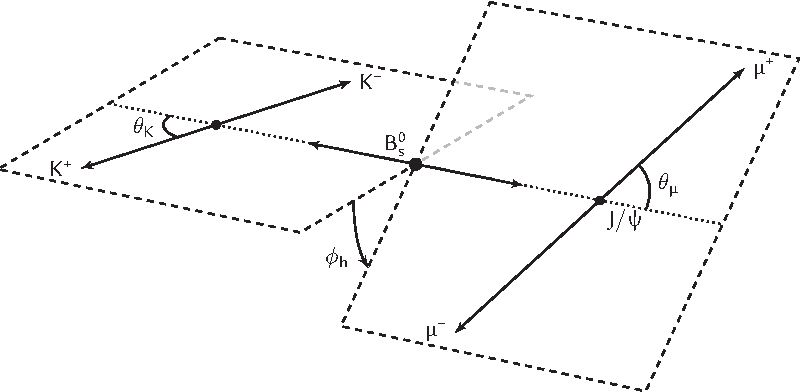
\includegraphics[width=\textwidth]{graphics/pheno/tikz/helAngles-crop}
  \caption{Decay angles in the helicity formalism (figure from \cite{Suvayu}).}
  \label{fig:helAngles}
\end{figure}

The change of variables from $\mpsiK^\text{2}$ and $\mKK^\text{2}$ to $\mKK$ and $\cthetaK$ introduces a Jacobian determinant in
Equation~\ref{eq:diffRateMsq}. Given that $\mKK^\text{2}$ does not depend on $\cthetaK$ when expressed in terms of the new variables, this
determinant reads $\frac{\partial\mKK^2}{\partial\mKK}\,\frac{\partial\mpsiK^2}{\partial\cthetaK}$. Exploiting kinematic relations between
the final-state momenta an expression for $\mpsiK^2$ can be derived:
\begin{equation}
  \mpsiK^2 = \tfrac{1}{2}\,(\mBs^2 + \mJpsi^2 + 2\,\mK^2 - \mKK^2) + 2\,\frac{\mBs}{\mKK}\,|\pJpsi|\,|\pK|\,\cthetaK \ ,
\end{equation}
where $\mBs$ is the $\Bs$ mass, $\pJpsi$ the $\Jpsi$ three-momentum in the rest frame of the $\Bs$, and $\pK$ the kaon three-momentum in
the $\KK$ rest frame.  With the derivative of this expression with respect to $\cthetaK$ the determinant is given by
$\text{4}\,\mBs\,|\pJpsi|\,|\pK|$. Including the determinant, ignoring constant factors, the differential decay rate can now be expressed
as
\begin{equation}
  \label{eq:diffRateAngles}
  \ud\Gamma \propto |\pJpsi|\,|\pK|\, |\mathcal{A}(\Bstof)|^2\, \ud\mKK\, \ud\cthetaK\, \ud\cthetal\, \ud\phihel \ .
\end{equation}
The factors $|\pJpsi|$ and $|\pK|$ depend on the $\KK$ invariant mass, but not on the decay angles and can be absorbed in the
$\mKK$-dependent part of $|\mathcal{A}(\Bstof)|^2$ (see Section~\ref{sec:pheno_KKMass}).

The squared amplitude for the \BstoJpsiKK{} process can be obtained by working out expressions for $|\Af|^2$, $|\Abarf|^2$ and
$\Af^*\,\Abarf$ and combining these with the decay time dependence of Equation~\ref{eq:mixDecayDiffRate}. The resulting expression is
ordered by the four time-dependent functions, $\cDGs$, $\sDGs$, $\cDms$, and $\sDms$. Each of the four function coefficients depends on the
kinematic variables. See Reference~\cite{Zhang:2012zk} for an example of this approach for $\text{B}_q^\text{0}\to\Jpsihh$ processes in
general.

However, it is often more convenient to order terms in the expression for the differential decay rate by intermediate resonant or
angular-momentum state rather than by decay-time dependence. Each term then has a distinct dependence on kinematic variables. For the
CP-violation analysis, a set of intermediate CP eigenstates is used to describe the decay.

The \BstoJpsiphi{} process is the decay of a spin-zero particle into two spin-one particles, which gives three intermediate
angular-momentum states. Describing the decay in terms of linear spin-polarization, or \emph{transversity} states, there is one state where
the polarization vectors of the $\Jpsi$ and the $\phimesalt$ point along the helicity axis and there are two states where the vectors are
transverse with respect to the helicity axis. The former polarization is called \emph{longitudinal} and is indicated with ``0''. The two
transverse polarizations are \emph{parallel} (``$\parallel$'') and \emph{perpendicular} (``$\perp$''), indicating the relative orientations
of the two vectors in the transverse plane.

The behaviour of the $\Jpsiphi$ system under a CP transformation depends on its orbital angular-momentum configuration. Since both the
$\Jpsi$ and the $\phimes$ particles are odd under a CP transformation, the CP of the system is equal to the parity of the orbital
angular-momentum state. For the longitudinal and parallel polarizations the state of the $\Jpsiphi$ orbital angular momentum is either an
S-wave ($L$\texteq0) or a D-wave ($L$\texteq2), which are even under a parity transformation. The perpendicular polarization state
corresponds to a P-wave ($L$\texteq1), which is odd under parity.

A fourth intermediate state is formed by the $\KK$ S-wave, indicated with ``S''. For this state the $\KK$ system has no angular momentum.
Because the decaying $\Bs$ meson is spinless, the orbital angular momentum of the $\JpsiKK$ system needs to be in a P-wave configuration,
which compensates for the spin of the $\Jpsi$. As a result, the $\KK$ S-wave state is odd under CP.

To derive an expression for the squared amplitude in terms of intermediate states it is necessary to go back to the expression for the
$\Bstof$ amplitude in Equation~\ref{eq:mixDecayAmps} and expand the decay amplitudes:
\begin{equation}
  \mathcal{A}(\Bstof) \propto g_+\, \Af + \qp\, g_-\, \Abarf = g_+\, \sum_i\Af[i] + \qp\, g_-\, \sum_j\Abarf[j]
  \ ,
\end{equation}
where $\Af[i]$ and $\Abarf[j]$ are the amplitudes for the $\Bsst$ and $\Bsbarst$ decays through intermediate states $i$ and $j$,
respectively. The dependence of the $\Bsst$ decay amplitude on final state kinematics is given by
\begin{equation}
  \label{eq:decayAmp}
  \Af[i] = \Ai\; \angAmp(\Omega)\; \mKKAmp(\mKK) \ ,
\end{equation}
where $\Ai$ is the complex-valued coefficient for amplitude $\Af[i]$ (also termed \emph{transversity amplitude}), $\angAmp$ is the
amplitude's dependence on decay angles (denoted by $\Omega$), and $\mKKAmp$ is a model of the dependence on the $\KK$ invariant mass.

The $\Bsbarst$ decay proceeds through the same intermediate states as the $\Bsst$ decay and the respective amplitudes have the same
kinematic dependence. Therefore, the $\Bsbarst$ amplitude is obtained by replacing the coefficient $\Ai$ with $\Abari$. The total $\Bstof$
amplitude can now be expressed as
\begin{equation}
  \label{eq:amplitudeAmpLami}
  \mathcal{A}(\Bstof) \propto \sum_i \left( g_+ + \lamsi\, g_- \right) \Af[i] = \sum_i \timeAmp\,\Af[i]
  \ ,
\end{equation}
where $\timeAmp$\textequiv$g_+ + \lamsi\, g_-$ represents the decay-time dependence and the parameter $\lamsi$ is defined in
accordance with $\lamf$ (Equation~\ref{eq:mixDecayLamfDef}):
\begin{equation}
  \label{eq:amplitudeLamiDef}
  \lamsi\equiv\qp\frac{\Abari}{\Ai}
\end{equation}
The amplitude for the $\Bsbartof$ decay is obtained by interchanging $g_+$ and $g_-$ and multiplying by a factor $\pq$ (see
Equation~\ref{eq:mixDecayAmps}). Notice that this only affects the decay-time part of Equation~\ref{eq:amplitudeAmpLami}, i.e. the factor
$\timeAmp$.

For intermediate CP eigenstates, the parameter $\lamsi$ can be expressed as
\begin{equation}
  \label{eq:amplitudeLamiParam}
  \lamsi = \eta_i\,\lamsiAbs\,e^{-i\,\phisi} \ ,
\end{equation}
where $\eta_i$\texteq\tpm1 is the CP eigenvalue of the state, $\lamsiAbs$\texteq$\qpAbsAlt\big|\frac{\Abari}{\Ai}\big|$, and the
CP-violating phase $\phisi$ is given by $\phisi\text{\textequiv\tm}\arg\big(\frac{1}{\eta_i}\lamsi\big)$. If CP symmetry is violated by
the same amount for all intermediate states, the combination $\frac{1}{\eta_i}\lamsi$ does not depend on the state and $\phisi\to\phis$.

Squaring the magnitude of $\mathcal{A}(\Bstof)$ gives an expression that contains products of the terms in
Equation~\ref{eq:amplitudeAmpLami} of the form $\Ai^*\Ai[j]\,\timeAmp^*\timeAmp[j]\, \angAmp^*\angAmp[j]\, \mKKAmp^*\mKKAmp[j]$.
Combining terms with indices $ij$ and $ji$, which are each others complex conjugates, gives
\begin{equation}
  \label{eq:sqAmp}
  |\mathcal{A}(\Bstof)|^2
    \propto \sum_i |\Ai\,\timeAmp\,\angAmp\,\mKKAmp|^2
      + \sum_{i\neq j} \Re( \Ai^*\Ai[j]\,\timeAmp^*\timeAmp[j]\, \angAmp^*\angAmp[j]\, \mKKAmp^*\mKKAmp[j] ) \ ,
\end{equation}
where the indices $i$ and $j$ run over the intermediate states $0$, $\parallel$, $\perp$, and S. The first sum in this expression contains
the \emph{diagonal terms} with the squared magnitude of the contribution of each state and the second sum contains the \emph{interference
terms} for the different combinations of two states. The dependence on decay time, decay angles, and invariant $\KK$ mass of this
expression are discussed in the following sections.

\section{Decay-Time Distribution}
\label{sec:pheno_time}

The distribution in decay time follows from the products $\timeAmp^*\timeAmp[j]$ (Equation~\ref{eq:amplitudeAmpLami}). With $|g_\pm|^2$ and
$g_+^*\,g_-$ from Equation~\ref{eq:mixDecayQpSq}, these products are given by
\begin{align}
  \timeAmp^*\timeAmp[j]
  &=\left[ |g_+|^2 + \lamsi^*\,\lamsi[j]\, |g_-|^2 + \lamsi^*\, (g_+^*\,g_-)^* + \lamsi[j]\, g_+^*\,g_- \right] \nonumber \\
  &=\tfrac{1}{2}\, \eGst\, \Big[    (1+\lamsi^*\lamsi[j]) \, \cDGs
                                +   (1-\lamsi^*\lamsi[j]) \, \cDms \nonumber \\
  &\quad\quad            -   (\lamsi^* + \lamsi[j])\,   \sDGs
                                - i (\lamsi^* - \lamsi[j])\,   \sDms \Big] \ .
\end{align}
Defining
\begin{equation}
  \label{eq:CDSPolarDep}
  \begin{aligned}
    \Cf[ij]^\pm    &\equiv \frac{1\pm\lamsi^*\lamsi[j]}{\sqrt{(1+\lamsiSq)(1+\lamsiSq[j])}} \\
    \qquad \Df[ij] &\equiv \frac{-    (\lamsi^* + \lamsi[j])}{\sqrt{(1+\lamsiSq)(1+\lamsiSq[j])}} \\
    \qquad \Sf[ij] &\equiv \frac{+i\, (\lamsi^* - \lamsi[j])}{\sqrt{(1+\lamsiSq)(1+\lamsiSq[j])}}
  \end{aligned}
\end{equation}
in accordance with Equation~\ref{eq:mixDecayCDS} and a ``CP-average'' decay amplitude
\begin{equation}
  \label{eq:CPAvAmp}
  \begin{gathered}
    \magAv \equiv \tfrac{1}{\sqrt{2}}\, \Ai\, \sqrt{1+\lamsiSq} \\
    \left|\magAv\right|^2
      = \tfrac{1}{2}\, |\Ai|^2\, \left(1 + \lamsiSq\right)
      = \tfrac{1}{2} \left(|\Ai|^2 + \qpAbsAlt^2\,|\Abari|^2\right) \ ,
  \end{gathered}
\end{equation}
the combination $\Ai^*\Ai[j]\,\timeAmp^*\timeAmp[j]$ can be expressed as
\begin{equation}
  \label{eq:timeDep}
  \begin{aligned}
    \Ai^*\Ai[j]\,\timeAmp^*\timeAmp[j]
      = \magAvConj&\magAv[{\Ai[j]}]\, \eGst \\
        \times\Big[ &\Cf[ij]^+\,\cDGs + \Cf[ij]^-\,\cDms \\
                    &+ \Df[ij]\,\sDGs - \Sf[ij]\,\sDms \Big] \ .
  \end{aligned}
\end{equation}

In general, the coefficients $\Cf[ij]^\pm$, $\Df[ij]$, and $\Sf[ij]$ are complex numbers and hence the terms
$\Ai^*\Ai[j]\,\timeAmp^*\timeAmp[j]$ have both real and imaginary parts. Notice that if $i=j$, the coefficients are real:
\begin{equation}
  \begin{alignedat}{2}
    \Cf[ii]^+ &= 1                                                    &  \Cf[ii]^- &= \frac{1-\lamsiSq}{1+\lamsiSq} \\
    \Df[ii]   &= -\frac{2\,\Re(\lamsi)}{1+\lamsiSq} \qquad\qquad  &  \Sf[ii]   &= \frac{2\,\Im(\lamsi)}{1+\lamsiSq} \ ,
  \end{alignedat}
\end{equation}
as required by the relation $\Ai^*\Ai^{\phantom{*}}\,\timeAmp^*\timeAmp^{\phantom{*}} = |\Ai\,\timeAmp|^2$.

The equivalent expression for the $\Bsbartof$ decay is obtained by changing the signs of the $\cDms$ and $\sDms$ terms and multiplying
by a factor $\pqAbsAlt^\text{2}$ (see Equations~\ref{eq:mixDecayAmps} and \ref{eq:mixDecayQpSq}). Using the definitions of $\qf$ and
$\Cm$ from Equations~\ref{eq:mixDecayDiffRateAll} and \ref{eq:CmDef}, the time dependence of the $\Bstof$ and $\Bsbartof$ decays is
given by
\begin{equation}
  \label{eq:timeqfDep}
  \begin{aligned}
    \Ai^*\Ai[j]\,\timeAmp[i,\qf]^*\timeAmp[j,\qf]^{\phantom{*}} =
      \magAvConj&\magAv[{\Ai[j]}]\, \frac{1-\qf\,\Cm}{1+\Cm}\, \eGst \\
          \times\Big[ &\Cf[ij]^+\,\cDGs + \qf\,\Cf[ij]^-\,\cDms \\
                      &+ \Df[ij]\,\sDGs - \qf\,\Sf[ij]\,\sDms \Big] \ .
  \end{aligned}
\end{equation}


%%%%%%%%%%%%%%%%%%%%%%%%%%%%%%%%%%%
\subsection{Parameterization}
\label{subsec:pheno_time_param}
%%%%%%%%%%%%%%%%%%%%%%%%%%%%%%%%%%%

% phi_s and C_s parameters, |lambda_s| used for historical reasons, approximations

\begin{equation}
  \begin{aligned}
    \label{eq:timeCPEvenOdd}
    \timeAmp[i,+1]^*\timeAmp[i,+1]^{\phantom{*}} + \timeAmp[i,-1]^*\timeAmp[i,-1]^{\phantom{*}}
      &\propto \eGst\left[ \cDGs - \eta_i\,\sDGs \right]  \\
      &= \left\{\begin{array}{ll}
                  e^{-\GL\,t}  &  \text{if } \eta_i = +1 \text{ (CP even)}  \\
                  e^{-\GH\,t}  &  \text{if } \eta_i = -1 \text{ (CP odd)}
         \end{array}\right.
  \end{aligned}
\end{equation}

\begin{equation}
  \label{eq:timeOscill}
  \timeAmp[i,+1]^*\timeAmp[i,+1]^{\phantom{*}} - \timeAmp[i,-1]^*\timeAmp[i,-1]^{\phantom{*}}
    \propto \eGst\left[ \Csi\,\cDms + \eta_i\,\phisi\,\sDms \right]
\end{equation}



%%%%%%%%%%%%%%%%%%%%%%%%%%%%%%%%%%%%%%%%%
\subsection{Alternative Parameterization}
\label{subsec:pheno_time_altParam}
%%%%%%%%%%%%%%%%%%%%%%%%%%%%%%%%%%%%%%%%%
The coefficients of the time-dependent functions in Equation~\ref{eq:timeqfDep} are functions of $\lamsi$ and hence contain both the
effects of CP violation in mixing and CP violation in decay. These two effects can be separated with an alternative parameterization.
Defining
\begin{equation}
  \label{eq:decayRho}
  \begin{gathered}
    \Ppm \equiv \frac{1}{2} \left[ 1 \pm \left(\frac{\Abari}{\Ai}\right)^{\!*}\, \frac{\Abari[j]}{\Ai[j]} \right] \\[0.6em]
    \Pre \equiv \frac{1}{2} \left[ \left(\frac{\Abari}{\Ai}\right)^{\!*} + \frac{\Abari[j]}{\Ai[j]} \right] \quad\quad
    \Pim \equiv \frac{i}{2} \left[ \left(\frac{\Abari}{\Ai}\right)^{\!*} - \frac{\Abari[j]}{\Ai[j]} \right]
  \end{gathered}
\end{equation}
and
\begin{equation}
  \label{eq:mixCDS}
  \Cm \equiv \frac{1-\qpAbsAlt^2}{1+\qpAbsAlt^2}
  \qquad \Dm \equiv -\frac{2\,\Re\big(\qpAlt\big)}{1+\qpAbsAlt^2}
  \qquad \Sm \equiv  \frac{2\,\Im\big(\qpAlt\big)}{1+\qpAbsAlt^2}
  \ ,
\end{equation}
the product $\Ai^*\Ai[j]\,\timeAmp[i,\qf]^*\timeAmp[j,\qf]^{\phantom{*}}$ can be expressed as
\begin{equation}
  \label{eq:timeqfDepSep}
  \begin{aligned}
    \Ai^*\Ai[j]\,\timeAmp[i,\qf]^*\timeAmp[j,\qf]^{\phantom{*}} =
      \Ai^*&\Ai[j]\, \frac{1-\qf\,\Cm}{1-\Cm^2}\, \eGst \\
        \times\Big[ &(\Ppl+\Pmn\,\Cm)\,\cDGs \\
                    &\quad + \qf\,(\Pmn+\Ppl\,\Cm)\,\cDms \\
                    &\quad\quad + (\Pre\,\Dm+\Pim\,\Sm)\,\sDGs \\
                    &\quad\quad\quad + \qf\,(\Pim\,\Dm-\Pre\,\Sm)\,\sDms \Big] \ .
  \end{aligned}
\end{equation}

Since the phases of $\qp$ and $\frac{\Abari}{\Ai}$ cannot be observed independently, only the combinations $\Pre\,\Dm$\textplus$\Pim\,\Sm$
and $\Pim\,\Dm$\textminus$\Pre\,\Sm$ are observable and not the $\Pre$, $\Pmn$, $\Dm$, and $\Sm$ parameters individually. A phase
convention can be chosen by, for example, setting $\arg(\qpAbsAlt)$\textequiv0, which makes the phase of $\frac{\Abari}{\Ai}$ equal
to the phase of $\lamsi$. Another choice is $\arg(\frac{\Abari[\text{0}]}{\Ai[\text{0}]})$\textequiv0,
which results in $\arg(\qpAbsAlt)$\texteq$\arg(\lamsi[\text{0}])$ and
$\arg(\frac{\Abari}{\Ai})$\texteq$\arg(\lamsi)$\textminus$\arg(\lamsi[\text{0}])$ and enables a measurement of phase differences.


\section{Decay-Angle Distributions}
\label{sec:pheno_angles}

\section{Invariant \texorpdfstring{$\KK$}{KK}-Mass Distribution}
\label{sec:pheno_KKMass}

\section{Decay-Rate Equations}
\label{sec:pheno_equations}

Combining the expressions for the decay-time and $\KK$-mass dependence from Equations~\ref{eq:timeDep} and \ref{eq:couplingFacAmps} yields
the coefficients in the sum of the angular dependence in Equation~\ref{eq:sqAmpExpand}:
\begin{equation}
  \begin{aligned}
    \label{eq:angCoefs}
    &\int_{\mKK^-}^{\mKK^+}\ud\mKK\,|\pJpsi|\,|\pK|\, c_i^*c_j
      = \int_{\mKK^-}^{\mKK^+}\ud\mKK\,|\pJpsi|\,|\pK|\, \Ai^*\Ai[j]\, \timeAmp^*\,\timeAmp[j]\, \mKKAmp^*\,\mKKAmp[j] \\
      &\quad\ \ = \Kij\, e^{-i\kij}\, \AAvConj\AAv[{\Ai[j]}]\, \eGst
              \Big[ \Cf[ij]^+\,\cDGs + \Cf[ij]^-\,\cDms \\
              &\qquad\qquad\qquad\qquad\qquad\qquad\quad\ \
               + \Df[ij]\,\sDGs - \Sf[ij]\,\sDms \Big] \ .
  \end{aligned}
\end{equation}
The phase of the integral over the $\KK$-mass functions can be absorbed in the phase difference between the amplitudes, as in
Equation~\ref{eq:couplingFacAmps}:
\begin{equation}
  \begin{aligned}
    e^{-i\kij}\, \AAvConj\AAv[{\Ai[j]}]
      &= |\AAv|\,|\AAv[{\Ai[j]}]|\, e^{i(\delta_j-\delta_i)} \\
      &= |\AAv|\,|\AAv[{\Ai[j]}]|\, [ \cos(\delta_j-\delta_i) + i\,\sin(\delta_j-\delta_i) ]\ ,
  \end{aligned}
\end{equation}
where
\begin{equation}
  \delta_j - \delta_i \equiv \arg(\AAv[{\Ai[j]}]) - \arg(\AAv) - \kij\ .
\end{equation}

Depending on whether the real or imaginary part of the coefficient is required in Equation~\ref{eq:sqAmpExpand}, the real and imaginary
parts of the time-dependence of Equation~\ref{eq:angCoefs} is multiplied by either $\cos(\delta_j-\delta_i)$ or $\sin(\delta_j-\delta_i)$.
Taking the $\cDGs$ term as an example, the coefficients of the angular distribution are proportional to
\begin{subequations}
  \label{eq:angCoefsReIm}
  \begin{align}
    \label{eq:angCoefsRe}
    \Re\!\big(e^{i(\delta_j-\delta_i)}\, \Cf[ij]^+ \big)
      &= \cos(\delta_j-\delta_i)\, \Re(\Cf[ij]^+) - \sin(\delta_j-\delta_i)\, \Im(\Cf[ij]^+) \\
    \label{eq:angCoefsIm}
    \Im\!\big(e^{i(\delta_j-\delta_i)}\, \Cf[ij]^+ \big)
      &= \sin(\delta_j-\delta_i)\, \Re(\Cf[ij]^+) + \cos(\delta_j-\delta_i)\, \Im(\Cf[ij]^+)\ ,
  \end{align}
\end{subequations}
where the first equation applies to the diagonal terms and the ``0$\parallel$'', ``0S'', and ``$\parallel$S'' terms and the second equation
to the ``0$\perp$'', ``$\parallel\perp$'', and ``$\perp$S'' terms.

The full expression for the differential decay rate in decay time and decay angles is obtained by summing the products of the angular
functions (Table~\ref{tab:angDist}) and their time-dependent coefficients (real or imaginary part of Equation~\ref{eq:angCoefs}). This
expression is used to build the probability density function that models the \BstoJpsiKK{} decay, as will be discussed in
Chapter~\ref{chap:ana}.


%%%%%%%%%%%%%%%%%%%%%%%%%%%%%%%%%%%%%%%%%%%%%%%%%
\subsection{Approximate Equations}
\label{subsec:pheno_equations_approx}
%%%%%%%%%%%%%%%%%%%%%%%%%%%%%%%%%%%%%%%%%%%%%%%%%

To indicate where the sensitivity to the different parameters in the decay model comes from, two approximations of the terms in the
differential rate are given in Tables~\ref{tab:timeFunctionsNoCPV}, \ref{tab:timeFunctionsApprox}, and \ref{tab:timeFunctionsApproxEqual}.
The first table shows the time-dependent functions in the differential decay rate in the case of no CP violation. Since CP violation in the
\BstoJpsiKK{} decay is small, this gives a good indication of how the remaining parameters appear in the decay-rate equations. Without CP
violation, the parameters $\Cs$ and $\Ss$ are equal to zero and $\Ds$ is equal to minus one. With Equation~\ref{eq:CDSPolarToCommon}, this
gives
\begin{subequations}
  \label{eq:CDSPolarToNoCPV}
  \begin{alignat}{5}
    \label{eq:CDSPolarToNoCPVEqual}
    \Cf[ij]^+ &\to  1      \quad\ \ &
    \Cf[ij]^- &\to  0      \quad\ \ &
    \Df[ij]   &\to -\eta_i \quad\ \ &
    \Sf[ij]   &\to  0      \quad&
    (\eta_i&=+\eta_j)      \\
    \label{eq:CDSPolarToNoCPVNotEqual}
    \Cf[ij]^+ &\to 0         \quad\ \ &
    \Cf[ij]^- &\to 1         \quad\ \ &
    \Df[ij]   &\to 0         \quad\ \ &
    \Sf[ij]   &\to i\,\eta_i \quad&
    (\eta_i&=-\eta_j)        \ .
  \end{alignat}
\end{subequations}

\begin{table}[htb]
  \centering
  \caption{Functions of decay time without CP violation.}
  \label{tab:timeFunctionsNoCPV}
  \renewcommand{\arraystretch}{1.3}
  \begin{tabular}{cl}
    \hline
    $ij$  &  $f(t) \times e^{+\Gs\,t}$  \\
    \hline
    $ii$
      &  $|\AAv|^2 \left[ \cDGs - \eta_i\,\sDGs \right]$  \\
    0$\parallel$
      &  $\magzeroAv\magparAv\cos(\delparzero) \left[ \cDGs - \sDGs \right]$  \\
    0$\perp$
      &  $\magzeroAv\magperpAv \left[ \sin(\delperpzero)\,\cDms - \cos(\delperpzero)\,\sDms \right]$  \\
    $\parallel\perp$
      &  $\magparAv\magperpAv \left[ \sin(\delperppar)\,\cDms - \cos(\delperppar)\,\sDms \right]$  \\
    0S
      &  $\CSP\magzeroAv\magSAv[i] \left[ \cos(\delSzero)\,\cDms + \sin(\delSzero)\,\sDms \right]$  \\
    $\parallel$S
      &  $\CSP\magparAv\magSAv \left[ \cos(\delSpar)\,\cDms + \sin(\delSpar)\,\sDms \right]$  \\
    $\perp$S
      &  $\CSP\magperpAv\magSAv\sin(\delSperp) \left[ \cDGs + \sDGs \right]$  \\
    \hline
  \end{tabular}
\end{table}

Equation~\ref{eq:CDSPolarToNoCPV} and Table~\ref{tab:timeFunctionsNoCPV} show that for terms with $\eta_i$\texteq$\eta_j$ only the $\cDGs$
and $\sDGs$ functions remain and for $\eta_i$\texteq\tm$\eta_j$ terms only the $\cDms$ and $\sDms$ functions. In the experiment,
flavour tagging is required to determine the coefficients of the latter, since these terms have opposite sign for $\Bs$ and $\Bsbar$ decays
(see Equation~\ref{eq:timeqfDep}) and cancel in the sum of the two differential decay rates. Because it is not possible to tag all decay
candidates (correctly), the statistical uncertainties of the associated parameters will generally be larger than the uncertainties of
parameters in the $\cDGs$ and $\sDGs$ terms.

Without CP violation, light and heavy eigenstates of the \BsBsbar{} system coincide with the CP-even and CP-odd states, respectively.
The time dependence of the diagonal terms, which form the decay-time distribution integrated over the decay angles, can consequently be
expressed as
\begin{equation}
  \begin{aligned}
    \label{eq:timeCPEvenOdd}
      |\AAv|^2\; \eGst&\left[ \cDGs - \eta_i\,\sDGs \right] \\
      &= \left\{\begin{array}{ll}
                  |\AAv|^2\; e^{-\GL\,t}  &  \text{if } \eta_i = +1 \quad\text{(CP even)}  \\
                  |\AAv|^2\; e^{-\GH\,t}  &  \text{if } \eta_i = -1 \quad\text{(CP odd)}
         \end{array}\right.
      \ .
  \end{aligned}
\end{equation}

The values of the parameters $\Gs$, $\DGs$, and $|\AAv|$ can be estimated relatively precisely from untagged decay candidates, but these
estimates are correlated. The mean of the decay-time distribution is controlled by $\Gs$, but also by the relative contributions of CP-even
and CP-odd states ($|\AAv|$), which have different lifetimes. The impact of changing the even and odd contributions depends on the value of
$\DGs$, which controls the difference in lifetime between the two states.

The phases of the transversity amplitudes can only be determined from interference terms. The cosine of $\delparzero$ and the sine of
$\delSperp$ appear in the untagged distribution, but tagged decay candidates are required to measure the sine of $\delparzero$ and the
cosine of $\delSperp$ from combinations of the remaining interference terms. As a result, the measurements of $\sin(\delparzero)$ and
$\cos(\delSperp)$ are less precise than the measurements of $\cos(\delparzero)$ and $\sin(\delSperp)$ and an approximate symmetry in the
estimates of these parameters arises for $\delparzero$\textto2$\pi$\textminus$(\delparzero)$ and
$\delSperp$\textto$\pi$\textminus$(\delSperp)$, for which the values of $\cos(\delparzero)$ and $\sin(\delSperp)$ do not change. The
parameter $\delperpzero$ is only determined with $\cDms$ and $\sDms$ terms in the approximation of Table~\ref{tab:timeFunctionsNoCPV} and
does not show a similar symmetry.

The interference term of the parallel and perpendicular states depends on both the $\delparzero$ and the $\delperpzero$ parameters:
\begin{subequations}
  \label{eq:parperpPhaseExp}
  \begin{align}
    \sin(\delperppar) &= \cos(\delparzero)\, \sin(\delperpzero) - \sin(\delparzero)\, \cos(\delperpzero) \nonumber\\
                      &\approx \sin(\delparzero) - \sin(\delperpzero)  \\
    \cos(\delperppar) &= \cos(\delparzero)\, \cos(\delperpzero) + \sin(\delparzero)\, \sin(\delperpzero) \nonumber\\
                      &\approx 1 \ .
  \end{align}
\end{subequations}
In these equations an approximation was used where the values of $\delparzero$ and $\delperpzero$ are approximately equal to $\pi$, which
is justified given previous measurements of these phase differences (see for example \cite{LHCb-PAPER-2013-002,*LHCb-ANA-2012-067}). The
combination of $\sin(\delparzero)$ and $\sin(\delperpzero)$ in the $\sDms$ coefficient of this term introduces a correlation between the
parameters $\delparzero$ and $\delperpzero$.

Since the fraction of S-wave is small, the sensitivity for the parameter $\Dms$ is expected to mainly come from the ``0$\perp$'' and
``$\parallel\perp$'' interference terms. The $\cDms$ and $\sDms$ functions in these terms can be combined into a single sine function with
a phase:
\begin{equation}
  \sin\delta\, \cDms - \cos\delta\, \sDms = -\sin\!\left(\Dms\,t - \delta \right) \ .
\end{equation}
Because a change in the frequency of a sine function in a limited range can be partially compensated by a phase shift, these terms
introduce correlations between $\Dms$ and the phases of the transversity amplitudes. Since practically all information on $\delperpzero$
comes from the ``0$\perp$'' and ``$\parallel\perp$'' terms, this parameter is affected most.

Table~\ref{tab:timeFunctionsApprox} shows the time dependence of the differential decay rate including CP violation, but with several
approximations for small parameters. Given previous measurements, it is known that CP violation in \BstoJpsiKK{} is small, which leads to
$\lamsiAbs$\textapprox1 and $\phisi$\textapprox0. To parameterize also CP violation in decay and CP violation in mixing with a small
parameter, $\lamsiAbs$ is replaced with
\begin{equation}
  \label{eq:CsDef}
  \Csi \equiv \Cf[ii]^- = \frac{1-\lamsiSq}{1+\lamsiSq} \ .
\end{equation}

An expansion in $\Csi$ and $\phisi$ is used for the approximation in Table~\ref{tab:timeFunctionsApprox}. Expanding the coefficients of the
decay-rate equations (Equation~\ref{eq:CDSPolarDep}) in terms of these parameters at first order yields
\begin{subequations}
\begin{equation}
  \begin{aligned}
    \Cf[ij]^+ &\approx 1 + i \cdot \tfrac{1}{2} (\phisi - \phisi[j]) \\
    \Cf[ij]^- &\approx \tfrac{1}{2} (\Csi + \Csi[j]) - i \cdot \tfrac{1}{2} (\phisi - \phisi[j]) \\
    \Df[ij]   &\approx -\eta_i \left[ 1 + i \cdot \tfrac{1}{2} (\phisi - \phisi[j]) \right] \\
    \Sf[ij]   &\approx -\eta_i \left[ i \cdot \tfrac{1}{2} (\Csi - \Csi[j]) + \tfrac{1}{2} (\phisi + \phisi[j]) \right]
  \end{aligned}
\end{equation}
for $\eta_i$\texteq$\eta_j$ and
\begin{equation}
  \begin{aligned}
    \Cf[ij]^+ &\approx \tfrac{1}{2} (\Csi + \Csi[j]) - i \cdot \tfrac{1}{2} (\phisi - \phisi[j]) \\
    \Cf[ij]^- &\approx 1 + i \cdot \tfrac{1}{2} (\phisi - \phisi[j]) \\
    \Df[ij]   &\approx +\eta_i \left[ \tfrac{1}{2} (\Csi - \Csi[j]) - i \cdot \tfrac{1}{2} (\phisi + \phisi[j]) \right] \\
    \Sf[ij]   &\approx +\eta_i \left[ i - \tfrac{1}{2} (\phisi - \phisi[j]) \right]
  \end{aligned}
\end{equation}
for $\eta_i$\texteq\tm$\eta_j$.
\end{subequations}

Also the value of $\DGs$ is small enough to allow an approximation of the $\cDGs$ and $\sDGs$ functions. A first-order expansion in $\DGs$
gives
\begin{equation}
  \cDGs \approx 1 \qquad \sDGs \approx \tfrac{1}{2}\DGs\,t \ .
\end{equation}

The sines and cosines of the phase differences $\delparzero$ and $\delperpzero$ are expanded around $\pi$, as in
Equation~\ref{eq:parperpPhaseExp}:
\begin{equation}
  \begin{alignedat}{4}
    &\sin(\delparzero)  &&\approx \pi - (\delparzero) \qquad\quad &&\cos(\delparzero)  &&\approx -1  \\
    &\sin(\delperpzero) &&\approx \pi - (\delperpzero)            &&\cos(\delperpzero) &&\approx -1  \\
    &\sin(\delperppar)  &&\approx \delperppar                     &&\cos(\delperppar)  &&\approx +1  \ .
  \end{alignedat}
\end{equation}
In the table, the remaining non-trivial sine and cosine functions are denoted by
\begin{equation}
  \sij{i}{j} \equiv \sin(\delta_j - \delta_i) \qquad\quad
  \cij{i}{j} \equiv \cos(\delta_j - \delta_i) \ .
\end{equation}

\begin{table}[p]
  \centering
  \caption{Functions of decay time with approximations for small CP violation, small $\DGs$, and phase differences close to 0 or $\pi$.}
  \label{tab:timeFunctionsApprox}
  \renewcommand{\arraystretch}{1.7}
  \begin{tabular}{cl}
    \hline
    $ij$  &  $f(t) \times e^{+\Gs\,t}$  \\
    \hline
    $ii$
      &  $|\AAv|^2 \Big[
                     1 - \tfrac{1}{2}\,\eta_i\,\DGs\,t
                     + \Csi\,\cDms + \eta_i\,\phisi\,\sDms
                   \Big]$  \\
    0$\parallel$
      &  $-\magzeroAv\magparAv \Big[
                             1 - \tfrac{1}{2}\,\DGs\,t$  \\
      &  $\qquad\qquad\quad  + \tfrac{1}{2}(\Cszero + \Cspar) \cDms + \tfrac{1}{2}(\phiszero + \phispar) \sDms
                           \Big]$  \\
    0$\perp$
      &  $-\magzeroAv\magperpAv \Big[
                              \tfrac{1}{2}(\phisperp-\phiszero) - \tfrac{1}{4}(\phiszero+\phisperp)\,\DGs\,t$  \\
      &  $\qquad\qquad\quad   - (\szeroperp + \tfrac{1}{2}\phisperp - \tfrac{1}{2}\phiszero) \cDms - \sDms
                            \Big]$  \\
    $\parallel\perp$
      &  $+\magparAv\magperpAv \Big[
                             \tfrac{1}{2}(\phisperp-\phispar) - \tfrac{1}{4}(\phispar+\phisperp)\,\DGs\,t$  \\
      &  $\qquad\qquad\quad  + (\sparperp - \tfrac{1}{2}\phisperp + \tfrac{1}{2}\phispar) \cDms - \sDms
                           \Big]$  \\
    0S
      &  $-\CSP\magzeroAv\magSAv \Big[
                           \tfrac{1}{2}(\Cszero+\CsS)\cperpS - \tfrac{1}{2}(\phisS-\phiszero)\sperpS$  \\
      &  $\qquad\qquad\quad    - \big[ \tfrac{1}{2}(\CsS-\Cszero)\cperpS - \tfrac{1}{2}(\phiszero+\phisS)\sperpS \big]
                                 \cdot\tfrac{1}{2}\DGs\,t$ \\
      &  $\qquad\qquad\quad\   + \big[ \cperpS + (\szeroperp + \tfrac{1}{2}\phisS - \tfrac{1}{2}\phiszero)\sperpS \big]\cDms$  \\
      &  $\qquad\qquad\quad\ \ - \big[ (\szeroperp + \tfrac{1}{2}\phisS - \tfrac{1}{2}\phiszero)\cperpS - \sperpS \big]\sDms
                         \Big]$  \\
    $\parallel$S
      &  $+\CSP\magparAv\magSAv \Big[
                           \tfrac{1}{2}(\Cspar+\CsS)\cperpS - \tfrac{1}{2}(\phisS-\phispar)\sperpS$  \\
      &  $\qquad\qquad\quad    - \big[ \tfrac{1}{2}(\CsS-\Cspar)\cperpS - \tfrac{1}{2}(\phispar+\phisS)\sperpS \big]
                                 \cdot\tfrac{1}{2}\DGs\,t$ \\
      &  $\qquad\qquad\quad\   + \big[ \cperpS - (\sparperp - \tfrac{1}{2}\phisS + \tfrac{1}{2}\phispar)\sperpS \big]\cDms$  \\
      &  $\qquad\qquad\quad\ \ + \big[ (\sparperp - \tfrac{1}{2}\phisS + \tfrac{1}{2}\phispar)\cperpS + \sperpS \big]\sDms
                         \Big]$  \\
    $\perp$S
      &  $-\CSP\magperpAv\magSAv \Big[
                           \big[ \tfrac{1}{2}(\phisS-\phisperp)\cperpS - \sperpS \big] (1 + \tfrac{1}{2}\DGs\,t)$ \\
      &  $\qquad\qquad\quad\   - \big[ \tfrac{1}{2}(\phisS-\phisperp)\cperpS + \tfrac{1}{2}(\Csperp + \CsS)\sperpS \big]\cDms$  \\
      &  $\qquad\qquad\quad\ \ - \big[ \tfrac{1}{2}(\CsS-\Csperp)\cperpS - \tfrac{1}{2}(\phisperp + \phisS)\sperpS \big]\sDms
                         \Big]$  \\
    \hline
  \end{tabular}
\end{table}

\begin{table}[tbp]
  \centering
  \caption{Functions of decay time with approximations for small CP violation, $\phisi$\textequiv$\phis$, $\Csi$\texteq$\Cs$,
           small $\DGs$, and phase differences close to 0 or $\pi$.}
  \label{tab:timeFunctionsApproxEqual}
  \renewcommand{\arraystretch}{1.7}
  \begin{tabular}{cl}
    \hline
    $ij$  &  $f(t) \times e^{+\Gs\,t}$  \\
    \hline
    $ii$
      &  $|\AAv|^2 \Big[
                     1 - \tfrac{1}{2}\,\eta_i\,\DGs\,t
                     + \Cs\,\cDms + \eta_i\,\phis\,\sDms
                   \Big]$  \\
    0$\parallel$
      &  $-\magzeroAv\magparAv \Big[
                                 1 - \tfrac{1}{2}\,\DGs\,t
                                 + \Cs\, \cDms + \phis\, \sDms
                               \Big]$  \\
    0$\perp$
      &  $+\magzeroAv\magperpAv \Big[
                                  \tfrac{1}{2}\,\phis\,\DGs\,t
                                  + \szeroperp\, \cDms + \sDms
                                \Big]$  \\
    $\parallel\perp$
      &  $-\magparAv\magperpAv \Big[
                                 \tfrac{1}{2}\,\phis\,\DGs\,t
                                 - \sparperp\, \cDms + \sDms
                               \Big]$  \\
    0S
      &  $-\CSP\magzeroAv\magSAv \Big[
                                   \Cs\,\cperpS
                                   + \tfrac{1}{2}\,\phis\,\sperpS\,\DGs\,t$ \\
      &  $\qquad                   + (\cperpS + \szeroperp\,\sperpS) \cDms
                                   - (\szeroperp\,\cperpS - \sperpS)\sDms
                                 \Big]$  \\
    $\parallel$S
      &  $+\CSP\magparAv\magSAv \Big[
                                  \Cs\,\cperpS
                                  + \tfrac{1}{2}\,\phis\,\sperpS\,\DGs\,t$ \\
      &  $\qquad                  + (\cperpS - \sparperp\,\sperpS)\cDms
                                  + (\sparperp\,\cperpS + \sperpS)\sDms
                                \Big]$  \\
    $\perp$S
      &  $+\CSP\magperpAv\magSAv \Big[
                                   \sperpS (1 + \tfrac{1}{2}\DGs\,t)$ \\
      &  $\qquad                   + \Cs\,\sperpS\,\cDms
                                   - \phis\,\sperpS\,\sDms
                                 \Big]$  \\
    \hline
  \end{tabular}
\end{table}

Integrating over the decay angles, the shape of the distribution of decay time is given by the sum of the diagonal terms in the
differential rate. As can be seen in Table~\ref{tab:timeFunctionsApprox}, CP violation only affects the oscillatory terms in this
distribution in the first-order approximation. These terms have opposite sign for $\Bs$ and $\Bsbar$ and can be isolated by taking the
difference between the two differential rates with $\qf$\texteq\tp1 and $\qf$\texteq\tm1 (see also Equation~\ref{eq:timeqfDep}). For a
single term, this difference is approximately given by
\begin{equation}
  \label{eq:timeOscill}
  \timeAmp[i,+1]^*\timeAmp[i,+1]^{\phantom{*}} - \timeAmp[i,-1]^*\timeAmp[i,-1]^{\phantom{*}}
    \propto \eGst\left[ \Csi\,\cDms + \eta_i\,\phisi\,\sDms \right] \ .
\end{equation}

The CP violation parameters also appear in the interference terms, which provides additional information on their values. This is
particularly noticeable in cases where the parameters appear in the coefficient of the $\cDGs$ function, which is approximately equal to
one and not suppressed by the small value of $\DGs$ or by the effects of imperfect flavour tagging. In most cases this contributes to the
estimates of the differences between the $\phisi$ parameters, but in the ``0S'' and ``$\parallel$S'' terms also the values of
$\Cszero$\textplus$\CsS$ and $\Cspar$\textplus$\CsS$.

Table~\ref{tab:timeFunctionsApproxEqual} shows the time dependence of the differential decay rate in the same approximation, but with the
additional requirement that CP violation is identical for all intermediate states. In this case the $\phisi$ differences vanish, but
$\Cszero$\textplus$\CsS$ and $\Cspar$\textplus$\CsS$ reduce to 2$\Cs$. As a result, a significant part of the sensitivity for $\Cs$ (or
$\lamsAbs$) comes from the ``0S'' and ``$\parallel$S'' terms, despite the small value of the S-wave amplitude.


%%%%%%%%%%%%%%%%%%%%%%%%%%%%%%%%%%%%%%%
\subsection{A Symmetry in the Equations}
\label{subsec:pheno_equations_symmetry}
%%%%%%%%%%%%%%%%%%%%%%%%%%%%%%%%%%%%%%%

In the limit of equal CP violation for all intermediate states (or small differences), Equation~\ref{eq:angCoefsReIm} reveals an
(approximate) symmetry in the decay-rate equations. As explained in Section~\ref{subsec:pheno_time_commonCPV}, simultaneously applying the
operations $\phis$\textto$\pi$\textminus$\phis$ and $\DGs$\textto\tm$\DGs$ is equivalent to taking the complex conjugates of the
coefficients $\Cf[ij]^\pm$, $\Df[ij]$, and $\Sf[ij]$ in this limit. The corresponding sign flip in the imaginary parts of the coefficients
can be cancelled by flipping the sign of either $\sin(\delta_j$\textminus$\delta_i)$ for Equation~\ref{eq:angCoefsRe} or
$\cos(\delta_j$\textminus$\delta_i)$ for Equation~\ref{eq:angCoefsIm}.

The specific structure of the appearance of real and imaginary parts of the products $c_i^*c_j$ in the angular coefficients in
Table~\ref{tab:angDist} enables the required sign flips in $\sin(\delta_j$\textminus$\delta_i)$ and $\cos(\delta_j$\textminus$\delta_i)$.
Simultaneously applying the operations $\phis$\textto$\pi$\textminus$\phis$, $\DGs$\textto\tm$\DGs$,
$\delparzero$\textto\tm$(\delparzero)$, $\delperpzero$\textto$\pi$\textminus$(\delperpzero)$, and
$\delSperp$\textto$\pi$\textminus$(\delSperp)$ does not change the value of the \BstoJpsiKK{} differential decay rate in the limit of equal
CP violation for all intermediate states. As a result, there is an alternative set of parameter values for each given set, for which the
decay model fits the experimental data equally well.

To resolve this discrete ambiguity, the measurement is performed in multiple bins of $\KK$ mass. Integrating over $\mKK$ within each bin
gives different values for the phase $\thetaSP$, which affects the value $\delSperp$ that is measured for each bin. Comparing the behaviour
of $\delSperp$ across the bins to what is expected from the $\KK$-mass models determines which of the two ambiguous sets of parameter
values corresponds to the physical situation~\cite{Xie:2009fs}.

Moving through the $\phimes$ resonance from low $\mKK$ to high $\mKK$, the phase of the $\phimes\to\KK$ contribution roughly increases by
$\pi$, while the phase of the $\fzero\to\KK$ contribution is approximately constant. As a result, the phase $\thetaSP$ is expected to
increase from bins at low $\mKK$ to bins at high $\mKK$ and the phase difference $\delSperp$ is expected to decrease. This behaviour has
been shown to correspond to a value of $\phis$ close to zero and a positive value of $\DGs$, as opposed to $\phis$ close to $\pi$ and
negative $\DGs$~\cite{LHCb-PAPER-2011-028,LHCb-PAPER-2013-002,*LHCb-ANA-2012-067}.


%%%%%%%%%%%%%%%%%%%%%%%%%%%%%%%%%%%%
\subsection{Parameterization}
\label{subsec:pheno_equations_param}
%%%%%%%%%%%%%%%%%%%%%%%%%%%%%%%%%%%%

As mentioned in Section~\ref{subsec:pheno_equations_approx}, the small parameter $\Csi$ (Equation~\ref{eq:CsDef}) is used instead of
$\lamsAbs$, in addition to $\phisi$. As can be seen from Table~\ref{tab:timeFunctionsApprox}, the actual CP-violation observables in the
(angles-integrated) decay-time distribution are the sums of $\Csi$ and $\phisi$, weighted by the squared magnitudes of the corresponding
transversity amplitudes. These observables form the coefficients of the oscillatory functions in the diagonal terms of the differential
decay rate. Ignoring contributions from interference terms, these are also the observables that are measured with the assumption that CP
violation is identical for all intermediate states.

To parameterize in terms of these CP-violation observables as much as possible, the following linear combinations are defined:
\begin{equation}
  \label{eq:CPVParamDef}
  \begin{alignedat}{2}
    \Csav      &\equiv \tfrac{1}{2}\Cszero + \tfrac{1}{4}\Cspar + \tfrac{1}{4}\Csperp \qquad\quad&
      \phisav       &\equiv \phiszero + \tfrac{1}{2}\phispar - \tfrac{1}{2}\phisperp \\
    \DelCspara &\equiv \Cspar  - \Cszero &
      \Delphispara  &\equiv \phispar - \phiszero \\
    \DelCsperp &\equiv \Csperp - \Cszero &
      \Delphisperpp &\equiv \phisperp - \tfrac{1}{2}\phiszero - \tfrac{1}{2}\phispar \\
    \CsavS     &\equiv \tfrac{1}{2}\Cszero + \tfrac{1}{2}\CsS &
      \DelphisS  &\equiv \phisS - \phiszero \\
  \end{alignedat}
\end{equation}
The parameters $\Csav$ and $\phisav$ are the observables measured in the angles-integrated time distribution, ignoring interference terms,
ignoring the S-wave, and approximating the ratio $\magzeroAvSq$\,:\,$\magparAvSq$\,:\,$\magperpAvSq$ by 2\,:\,1\,:\,1.  This last
approximation is justified by the values reported in reference~\cite{LHCb-PAPER-2013-002,*LHCb-ANA-2012-067}, which are given by
$\magzeroAvSq$\textapprox0.52, $\magparAvSq$\textapprox0.23, and $\magperpAvSq$\textapprox0.25. The normalization factors are chosen such
that $\Csav$\textto$\Cs$ and $\phisav$\textto$\phis$ in the case of equal CP violation for all states.

The remaining parameters are the differences between the parameters of the different states and the parameters of the longitudinal state,
with the exceptions of $\Delphisperpp$ and $\CsavS$. The parameter $\Delphisperpp$ is a combination of $\phisperp$\textminus$\phiszero$ and
$\phisperp$\textminus$\phispar$, which both appear as coefficients of $\cDGs$ in the interference terms. $\CsavS$ appears in the $\cDGs$
coefficient of the ``0S'' term. Using these parameters instead of $\phisperp$\textminus$\phiszero$ and $\CsS$\textminus$\Cszero$ reduces
correlations between the $\phisi$ parameters and between the $\Csi$ parameters, respectively.

In the case of equal CP violation for all intermediate states, the coefficients of the decay-time functions are given by (see also
Equation~\ref{eq:CDSCommon})
\begin{equation}
  \begin{aligned}
    \Cs &\equiv \frac{1-\lamsiSq[]}{1+\lamsiSq[]} \\
    \Ds &\equiv -\frac{2\,\Re(\lamsi[])}{1+\lamsiSq[]} = -\sqrt{1-\Cs^2}\, \cos\phis \approx -1 \\
    \Ss &\equiv +\frac{2\,\Im(\lamsi[])}{1+\lamsiSq[]} = -\sqrt{1-\Cs^2}\, \sin\phis \approx -\phis \ ,
  \end{aligned}
\end{equation}
where a first-order expansion in the parameters $\Cs$ and $\phis$ was used for the approximation. For historical reasons, the parameter
$\lamsAbs$ is used in this case instead of $\Cs$.

The magnitudes of the transversity amplitudes are parameterized by their squares, $|\AAv|^2$. Since only the shape of the time and angular
distributions are measured and not the absolute scale of the differential decay rate, the overall scale of the transversity amplitudes is
arbitrary. To fix the scale, the magnitudes of the amplitudes are multiplied by a common factor, such that the sum of the squares for the
$\Jpsiphi$ polarization states is equal to one:
\begin{equation}
  \label{eq:ampNorm}
  \magzeroAvSq + \magparAvSq + \magperpAvSq \equiv 1 \ .
\end{equation}
The parameters $\magzeroAvSq$ and $\magperpAvSq$ are used in the decay model and the value of $\magparAvSq$ follows from
Equation~\ref{eq:ampNorm}. This procedure makes the squared magnitudes of the $\Jpsiphi$ amplitudes essentially polarization fractions,
although one should keep in mind that these amplitudes are combinations of the $\Bs$ and $\Bsbar$ values, which also contain mixing
parameters (see Equation~\ref{eq:CPAvAmp}).

The magnitude of the S-wave amplitude is parameterized by a fraction, given by
\begin{equation}
  \FSAv \equiv \frac{\magSAvSq}{\magzeroAvSq + \magparAvSq + \magperpAvSq + \magSAvSq} = \frac{\magSAvSq}{1 + \magSAvSq} \ .
\end{equation}
As mentioned in Section~\ref{sec:pheno_KKMass}, the differences between the phases of the transversity amplitudes are parameterized by
$\delparzero$, $\delperpzero$, and $\delSperp$. Both the S-wave fraction and the phase difference between the S-wave and the $\Jpsiphi$
polarizations are measured in bins of $\KK$ mass to resolve the discrete ambiguity discussed in
Section~\ref{subsec:pheno_equations_symmetry}: $\FSAv[,b]$ and $\delSperp[,b]$.

Values of the parameters in the model are estimated by fitting the shape of the differential decay-rate equation to the \BstoJpsiKK{}
data. To be able to describe the experimental data several experimental effects have to be added to the model that was discussed in this
chapter. The final experimental model will be discussed in Chapter~\ref{chap:ana}.


\chapter{Data Analysis}
\label{chap:ana}

To extract the parameters that describe the \BstoJpsiKK{} decay from the experimental data, the model of decay time and decay angles, as
discussed in Chapter~\ref{chap:pheno}, is fitted to the distribution of decays in the data. Several experimental effects have to be taken
into account in this fit. Some of these effects, for instance the uncertainty in the measurement of the decay time, are included by
augmenting the theoretical model. Backgrounds, on the other hand, are dealt with by selecting signal-like decay candidates in the data and
by subtracting remaining background from the data after selection.

This chapter deals with the preparation of experimental data (Section~\ref{sec:ana_bkgSub}) and the model that can be used to fit these
data (Sections~\ref{sec:ana_time}--\ref{sec:ana_tagging}). Also the use of the decay model in the fit (Section~\ref{sec:ana_fit}) and in
simulation (Section~\ref{sec:ana_sim}) are discussed.

\section{Maximum-Likelihood Fit}
\label{sec:ana_fit}

The fit of the decay model to the data is an \emph{unbinned maximum-likelihood fit}. A probability density function (PDF) is constructed by
normalizing the expression for the differential decay rate, including experimental effects, by dividing by its integral over decay time and
decay angles. A likelihood function of the PDF parameters for one $\Bs$ decay is given by the PDF at the values of time and angles for
that decay. The likelihood function for the full sample of decays is given by the product of all individual likelihoods.

Parameter values are estimated by maximizing the likelihood function for the sample. In practice, the negative logarithm of the likelihood
function (NLL) is minimized to find the maximum likelihood. Instead of a product, the NLL is a sum of the contributions from individual
decays.

The shape of the NLL around the minimum can be approximated by a second order Taylor series, i.e. a parabola. Since the first derivative of
this function vanishes at the point where the NLL reaches its minimum, the approximation for a given parameter $\mu$ can be written in the
form
\begin{equation}
  \label{eq:NLLPara}
  \text{NLL}(\mu) \approx \frac{1}{2\,\sigma_\mu^2}\, (\mu-\hat{\mu})^2 + C \ ,
\end{equation}
where $\hat{\mu}$ is the value of parameter $\mu$ in the minimum, $\sigma_\mu$ determines the width of the NLL shape around the minimum,
and $C$ is the NLL value in the minimum. The width, $\sigma_\mu$, is (related to) the statistical uncertainty of the estimate of parameter
$\mu$. The wider the NLL shape around the minimum, the larger the value of $\sigma_\mu$ and thus the uncertainty.

It depends on the actual shape of the NLL how well it is approximated by a parabola away from the minimum. An important factor is the
number of decays that is used to build the NLL. With more data the statistical uncertainties of the parameter estimates become smaller and,
in general, the NLL becomes more parabolic within an interval of a few times the value of $\sigma_\mu$ around the minimum.

In case the distribution of parameter estimates $\hat{\mu}$ from different measurements is described by a Gaussian shape, the shape of the
NLL will be truly parabolic. In this case the parameter $\sigma_\mu$ is an estimate of the standard deviation of the $\hat{\mu}$
distribution, which can be used as a measure of the statistical uncertainty of a parameter estimate. The value of $\sigma_\mu$ is
determined from the second derivative of the NLL, which is given by $\frac{1}{\sigma_\mu^2}$.

If the shape of the NLL around its minimum is not sufficiently parabolic, a different measure of the statistical uncertainty may be used.
Commonly the (absolute) difference between the value of $\mu$ at the point where the NLL reaches a value of $\tfrac{1}{2}+C$ and
$\hat{\mu}$ is taken as the uncertainty. In the parabolic case the NLL reaches this point at $\hat{\mu}+\sigma_\mu$ and
$\hat{\mu}-\sigma_\mu$, which results in an uncertainty of $\sigma_\mu$, as expected. In a more general case this NLL value may be reached
on the left and the right of $\hat{\mu}$ at different distances, which results in an asymmetric uncertainty.

In some cases the shape of the NLL differs from a parabola too much to give a meaningful single estimate of the parameter value and a
corresponding uncertainty. The simplest way to provide an estimate of the value in these cases is to specify the interval bounded by the
values of $\mu$ at a given NLL value. Common NLL values are the values that a parabola would reach at $n\cdot\sigma_\mu$ from the minimum,
which are given by $\tfrac{1}{2}\,n^2+C$. Hence the intervals are referred to as ``$n$ sigma'' intervals.

In general the NLL is a function of more than one parameter. The distribution of parameter estimates in the parabolic approximation is
given by a multivariate Gaussian shape, which includes also correlations between the estimates. Both the uncertainties and the correlations
of the parameter estimates are estimated from the shape of the NLL in the minimum, by determining second derivatives for all pairs
of parameters.

The parabolic shape of Equation~\ref{eq:NLLPara} for a parameter $\mu$ is given by the minimum of the NLL at each $\mu$ value. In the
parabolic approximation the minimum for a given value of $\mu$ is reached at
\begin{equation}
  \frac{1}{\sigma_{\nu_i}}\, (\nu_i-\hat{\nu}_i)  = \rho_{\mu\nu_i}\, \frac{1}{\sigma_\mu}\, (\mu-\hat{\mu})
\end{equation}
for all the other parameters $\nu_i$, where $\rho_{\mu\nu_i}$ is the correlation coefficient between the parameters $\mu$ and $\nu_i$. The
resulting function of parameter $\mu$ is termed \emph{profiled NLL}, the second derivative of which is again equal to
$\frac{1}{\sigma_\mu^2}$.


%%%%%%%%%%%%%%%%%%%%%%%%%%%%%%%%%%%%%%%%%%%%%%%
\subsection{Fit with Weighted Decay Candidates}
\label{subsec:ana_fit_weights}
%%%%%%%%%%%%%%%%%%%%%%%%%%%%%%%%%%%%%%%%%%%%%%%

As will be described in Section~\ref{sec:ana_bkgSub}, the time and angular distribution for \BstoJpsiKK{} signal decays is obtained by
subtracting the background distribution from the distribution that is observed in the data. This is accomplished by adding background
decay-candidates to the sample with negative weights. In the NLL, the contribution of each decay candidate is then multiplied with the
value of its weight.

Although the position of the minimum of a weighted NLL still gives a good estimate of the values of the NLL parameters, the parameter
uncertainties cannot be estimated directly from the shape of the NLL at its minimum any more. This can be seen by considering a fit in
intervals of a given variable, where the observed number of decays in each interval is compared to the prediction of this number by a
model. The uncertainties in the estimates of the model parameters are now related to the uncertainties in the observed number of decays in
each interval.

For unweighted decays the distribution of the observed number of decays ($N$) is a Poisson distribution, for which both the mean and the
variance are given by the expected number in the interval ($\nu$). An estimate of the expected number of decays, $\hat{\nu}$, is given by
$N$ and an estimate of the corresponding uncertainty by the square root of the estimated variance, $\sqrt{N}$.

In a fit with weighted decay candidates, where each candidate counts with a weight $w_c$, the observed number of decays is replaced by the
sum of weights, $W$\textequiv$\sum_c w_c$. The estimate of $\nu$ is now also given by $W$, as expected, but the uncertainty is estimated by
$\sqrt{W}$, which cannot be correct. If all weights are multiplied by a constant number, $n$, the relative uncertainty in the estimate of
$\nu$ should not change, since no information was added to the data sample. This means that the absolute uncertainty should increase by a
factor $n$, as $\hat{\nu}$\texteq$W$ does. If the uncertainty is estimated by $\sqrt{W}$, it only increases by a factor $\sqrt{n}$.

The correct uncertainty estimate for the expected number of decays is given by the square root of $W'$\textequiv$\sum_c w_c^2$. Unlike
$\sqrt{W}$, $\sqrt{W'}$ increases by a factor $n$ if all weights are multiplied by this common factor. To obtain this estimate of the
uncertainty, the original estimate from the Poisson distribution should be divided by a factor $\sqrt{\alpha}$, where $\alpha$ is given by
\begin{equation}
  \alpha \equiv \frac{W}{W'} = \frac{\sum_c w_c}{\sum_c w_c^2} \ .
\end{equation}

In an unbinned maximum likelihood fit the correction factor $\alpha$ can be used to modify the shape of the NLL. Since the uncertainties
are estimated from the second derivatives of the NLL, which are given by $\frac{1}{\sigma_\mu^2}$ in the parabolic case, the NLL is
multiplied by a factor $\alpha$:
\begin{equation}
  \label{eq:NLLPara_alpha}
  \text{NLL}'(\mu) \approx \frac{\alpha}{2\,\sigma_\mu^2}\, (\mu-\hat{\mu})^2 + C' \ .
\end{equation}
This will make the shape of the parabola around the NLL minimum wider (if $\alpha$\textlt1) or narrower (if $\alpha$\textgt1). Notice that
this does not affect the position of the minimum, from which the parameter values are estimated.

Note that whereas the factor $\alpha$ is an exact correction for the uncertainty estimate of the expected number of decays in the above
example, it is only an approximate correction for the parameters in the NLL. The resulting uncertainties have to be checked by evaluating
the shape of the distribution of parameter estimates in simulated experiments, as will be discussed in Sections~\ref{sec:ana_sim} and
\ref{sec:result_paramEst}.

\section{Decay-Candidate Selection and Background}
\label{sec:ana_bkgSub}
%show mass-fit results in $\cthetal$ bins

While the decay model discussed in Chapter~\ref{chap:pheno} describes the \BstoJpsiKK{} signal, the time and angular distribution in the
experimental data contains both signal and background decay candidates. The background distribution is subtracted from the total
distribution in the data to be able to fit the model to the signal distribution. Since there are statistical uncertainties associated to
both the total distribution and the subtracted background distribution, however, the resulting uncertainties in the signal-parameter
estimates become larger with an increasing amount of background decay candidates. Therefore, a selection procedure is applied, designed to
reject as many background candidates as possible without removing too many signal candidates.


%%%%%%%%%%%%%%%%%%%%%%%%%%%%%
\subsection{Selection}
\label{subsec:ana_bkgSub_sel}
%%%%%%%%%%%%%%%%%%%%%%%%%%%%%

The decay-candidate selection procedure is briefly described here. See reference~\cite{Aaij:2015} for a detailed discussion.

As described in Section~\ref{subsec:intro_LHCb_Jpsiphi}, the first selection requirements are applied in the L0 trigger, which only selects
events with hits in the LHCb muon stations and particles with a sufficiently high (transverse) momentum. From the events that remain, the
HLT reconstructs and selects $\mumu$ pairs that are likely to originate from a $\Jpsi\to\mumu$ decay. Offline, the resulting
$\Jpsi\to\mumu$ candidates are matched to $\KK$ pairs to form \BstoJpsiKK{} decay candidates. The four tracks these candidates consist of
are required to be compatible with a $\Bs$ that was produced in the associated primary vertex and decayed at a decay time above a given
threshold.

In both HLT1 and HLT2 there are two different types of selections applied. The first type does not use any information on the distance that
the $\Bs$ travelled before it decayed and the second type does. Requiring a minimum flight distance reduces the fraction of
background candidates significantly, since all four tracks originate from the primary vertex for most combinatorial background, while the
tracks in a $\Bs$ decay originate from a secondary vertex at some distance from the primary vertex. However, the flight distance variable
is correlated with the decay time variable and requiring a minimum flight distance introduces a non-trivial selection efficiency as a
function of decay time. Therefore, the sets of selection criteria that use information on the flight distance are called \emph{decay-time
biasing} or \emph{biased}.

The unbiased HLT1 selection requires two oppositely charged muon candidates that are close enough to originate from one decay vertex and
have a $\mumu$ invariant mass greater than 2.7\unitsp\GeV. The biased HLT1 selection does not require a $\Jpsi$ candidate, but selects
single tracks with a perpendicular distance to any primary vertex greater than 0.1\unitsp{}mm. Both of these selections reduce the number
of selected events to a manageable level. Approximately 68\% of the decay candidates that are finally used in the fit is selected by both
the unbiased and biased selections, approximately 14\% exclusively by the unbiased selection, and approximately 19\% exclusively by the
biased selection.
% HLT1: 81% unbiased; about the same numbers for the signal

Both the unbiased and the biased HLT2 selections require $\Jpsi\to\mumu$ candidates with an invariant $\mumu$-mass within a window of
0.24\unitsp\GeV{} centred at the $\Jpsi$ mass of 3.10\unitsp\GeV. In addition, the biased selection requires a minimum \emph{decay-length
significance} (DLS) of three for the $\Jpsi$ candidate. The DLS is defined as the distance between the $\mumu$ vertex and the associated
primary vertex (\emph{decay length}) divided by the uncertainty on this distance. Since the decay length is a measure of the flight
distance of the $\Bs$, this requirement is decay-time biasing.

Without the minimum-DLS requirement the rate of events that pass the HLT2 selection would be too high to handle online. Therefore, the
rate of the unbiased selection is reduced by processing only a fraction of the events that pass the HLT1 selection. To keep the selection
unbiased, the processed events are randomly selected, without considering any information on the reconstructed particles. In the final
data sample that is used in the fit, the number of decay candidates that is exclusively selected by the unbiased HLT2 selection is three
per cent of the number of candidates selected by the biased selection. Considering only signal candidates, the unbiased HLT2 selection adds
one per cent to the total.

The method of modelling the non-trivial decay-time efficiency shape introduced by the biased HLT selections is discussed in
Section~\ref{subsec:ana_time_acc}. Because the unbiased HLT2 selection adds only few signal candidates to the final data sample, but
including these data complicates modelling of the efficiency significantly, only the time and angular distributions of HLT2-biased
candidates are fitted. However, candidates selected by the unbiased HLT2 selection are used to extract the efficiency shapes from the
\BstoJpsiKK{} data. The efficiencies of the biased selections are determined relative to the uniform efficiencies of the unbiased
selections. 

In the offline reconstruction process the muon tracks and the $\mumu$ vertex of $\Jpsi\to\mumu$ candidates selected by HLT2 are combined
into \BstoJpsiKK{} candidates with two oppositely charged kaons that form a $\KK$ vertex. The subsequent stripping selection imposes
requirements on how well detector hits form tracks within experimental uncertainties, how well tracks form $\mumu$, $\KK$, and $\mumu\,\KK$
vertices, the particle transverse momenta, the likelihood that the particles are identified correctly as muons and kaons, the invariant
masses of the reconstructed $\mumu$, $\KK$, and $\JpsiKK$ combinations, and the decay time of the candidate. About twelve million
\BstoJpsiKK{} candidates remain after this selection stage.

The selection of decay candidates is refined in the final offline stage. To visualize the effect of the selection, the distribution in
$\JpsiKK$ mass of remaining decay candidates is plotted for different selection requirements in Figure~\ref{fig:JpsiKKMassSel}. Notice that
the figure shows only a part of the mass range.
\begin{figure}[tb]
  \centering
  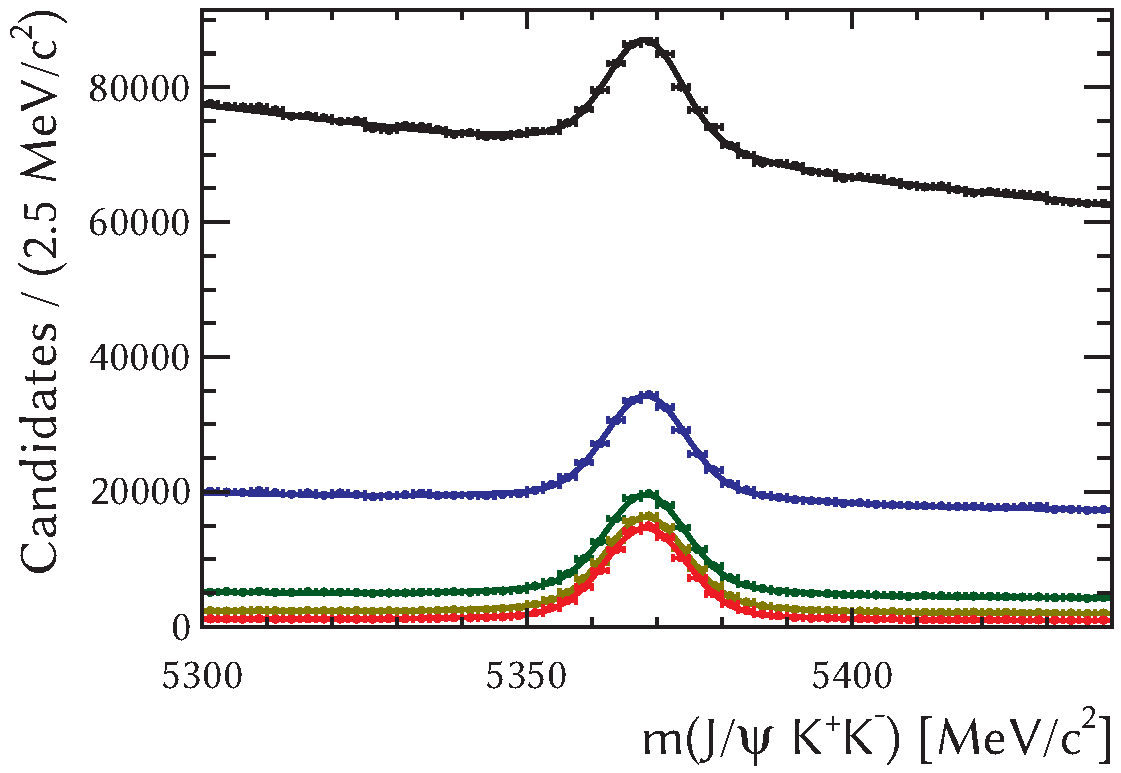
\includegraphics[width=0.7\textwidth]{graphics/analysis/JpsiKKMassSel}
  \caption{Distribution of \BstoJpsiKK{} decays in $\JpsiKK$ mass for different selection criteria.
           The data are shown as points, while the lines represent a model that consists of the sum of two Gaussian shapes (signal)
           and an exponential shape (combinatorial background).
           Subsequent selection criteria are applied in addition to previous criteria:
           black: stripping selection; blue: minimum quality of $\Bs$ decay-vertex reconstruction;
           green: minimum $\KK$ transverse momentum; yellow: minimum decay time; red: full offline selection.
           Notice that only a part of the total mass range is shown.}
  \label{fig:JpsiKKMassSel}
\end{figure}

For \BstoJpsiKK{} signal candidates this distribution is a peak around the value of the $\Bs$ mass of approximately 5367\unitsp\MeV. The
width of this peak is determined by the experimental resolution on the $\JpsiKK$-mass measurement. The background is mainly combinatorial
and follows an exponential distribution, which decays slowly across the considered mass range. Because of the obvious difference in
distributions of $\JpsiKK$ mass for the signal and the background, this variable can be used to statistically separate the two
contributions.

The distribution of black data points in Figure~\ref{fig:JpsiKKMassSel} is for candidates that pass the stripping selection without further
requirements. A peak of signal candidates is visible on top of a large background distribution. To determine the numbers of signal and
background candidates, the surface areas underneath the peak and the exponential distribution are determined with a fit. The signal peak is
modelled with the sum of a narrow ($\sigma$\textapprox6\unitsp\MeV) and wide ($\sigma$\textapprox16\unitsp\MeV) Gaussian shape and the
background with and exponential shape. The fit yields approximately 123 thousand signal candidates, which corresponds to a signal fraction
of approximately one per cent.

In the rest frame of the $\Bs$, the momentum of the $\KK$ pair is approximately 1.6\unitsp\GeVc{} for signal decays. Boosting into the
frame of the detector, approximately along the beam axis, this translates in a typical transverse momentum above 1\unitsp\GeVc. The sum of
the transverse momentum components of two kaons that accidentally form a suitable $\KK$ vertex in combinatorial background is often not
sufficient to make a transverse momentum of 1\unitsp\GeVc. As a result, requiring this value as a minimum in the offline selection removes
about 74\% of the background, but only 6\% of the signal, with respect to the stripping selection where already a minimum of
0.5\unitsp\GeVc{} was required. The $\JpsiKK$-mass distribution with the $\KK$ transverse momentum requirement is shown by the blue points
in Figure~\ref{fig:JpsiKKMassSel}.

To estimate the position of the $\Bs$ decay vertex and the kinematics of the particles in the decay as well as possible, these variables
are determined from a fit. The fit takes the position of the primary vertex, the muon and kaon tracks, and the corresponding experimental
uncertainties as inputs and minimizes a $\chi^2$ function for the position of the decay vertex and its perpendicular distance to the flight
path of the $\Bs$, which should be equal to zero. The value of the $\chi^2$ function in its minimum is a measure of the quality of the fit,
i.e. of how well the four reconstructed particles form a $\Bs$ decay vertex. The fit will in general be good for signal candidates, which
results in small values for the $\chi^2$ function.

Requiring a $\chi^2$ smaller than five times the number of degrees of freedom in the vertex fit removes about 75\% of the background that
remains after requiring a minimum $\KK$ transverse momentum of 1\unitsp\GeVc. Approximately 8\% of the remaining signal is lost. The
distribution of decay candidates after the $\KK$ transverse momentum and vertex fit quality requirements is shown by the green points in
Figure~\ref{fig:JpsiKKMassSel}.

A third requirement that removes a significant part of the background is a minimum on the reconstructed value of the decay time. For most
of the background candidates the four particles originate directly from the primary vertex, which corresponds to vanishing decay time
within experimental resolution. The stripping selection already requires a minimum decay time of 0.2\unitsp{}ps. Requiring a minimum of
0.3\unitsp{}ps in addition to the stripping selection and the $\KK$ transverse momentum and vertex fit $\chi^2$ requirements removes about
54\% of the remaining background and 6\% of the signal. The distribution for remaining candidates is shown by the yellow points in
Figure~\ref{fig:JpsiKKMassSel}.

Finally applying the full offline selection removes another 62\% of the background and 6\% of the signal, leaving approximately 94
thousand signal candidates and 135 thousand background candidates for further analysis. This corresponds to a signal fraction of 41\% in
the full $\JpsiKK$-mass range of 5200--5550\unitsp\MeV{} after the full selection.

The final $\JpsiKK$-mass distribution is shown by the red points in Figure~\ref{fig:JpsiKKMassSel} and also in
Figure~\ref{fig:JpsiKKMass_DG}. The latter figure shows the distribution both in the 5300--5440\unitsp\MeV{} mass range on a linear
vertical scale (left) and in the full mass range on a logarithmic vertical scale. The signal and combinatorial background contributions as
determined in the fit are shown separately.

\begin{figure}[tb]
  \centering
  \begin{subfigure}{0.49\textwidth}
    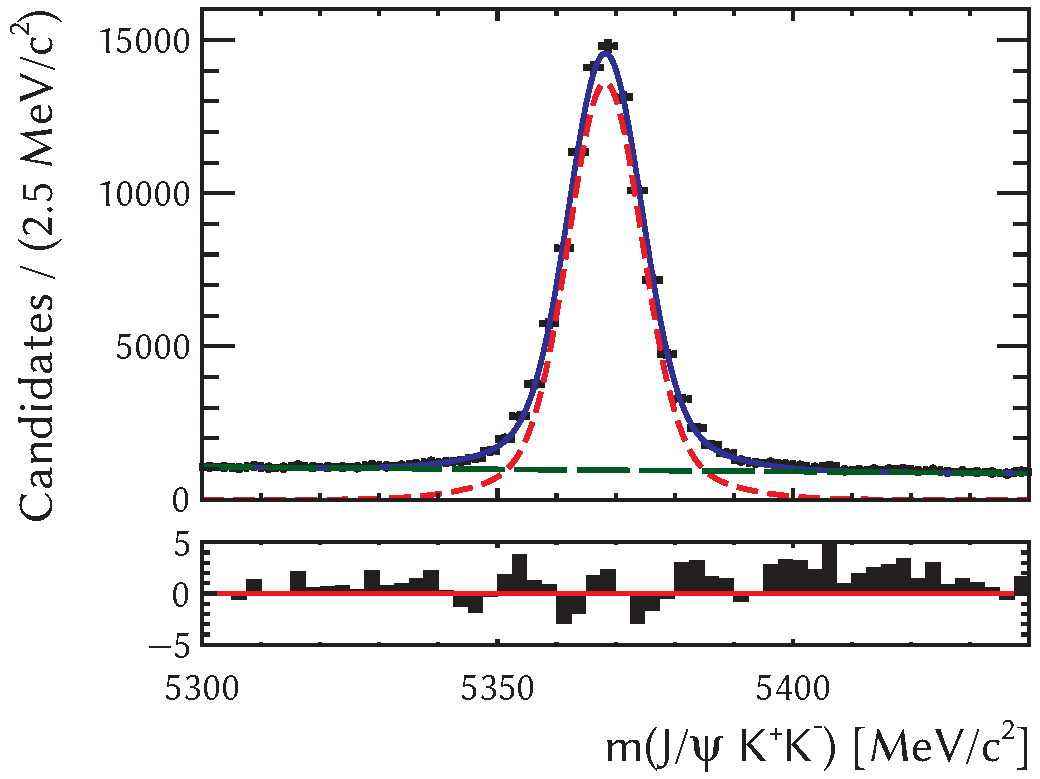
\includegraphics[width=\textwidth]{graphics/analysis/JpsiKKMass_DG_lin_resid}
    \caption{}
    \label{fig:JpsiKKMass_DG_lin}
  \end{subfigure}%
  \hfill%
  \begin{subfigure}{0.49\textwidth}
    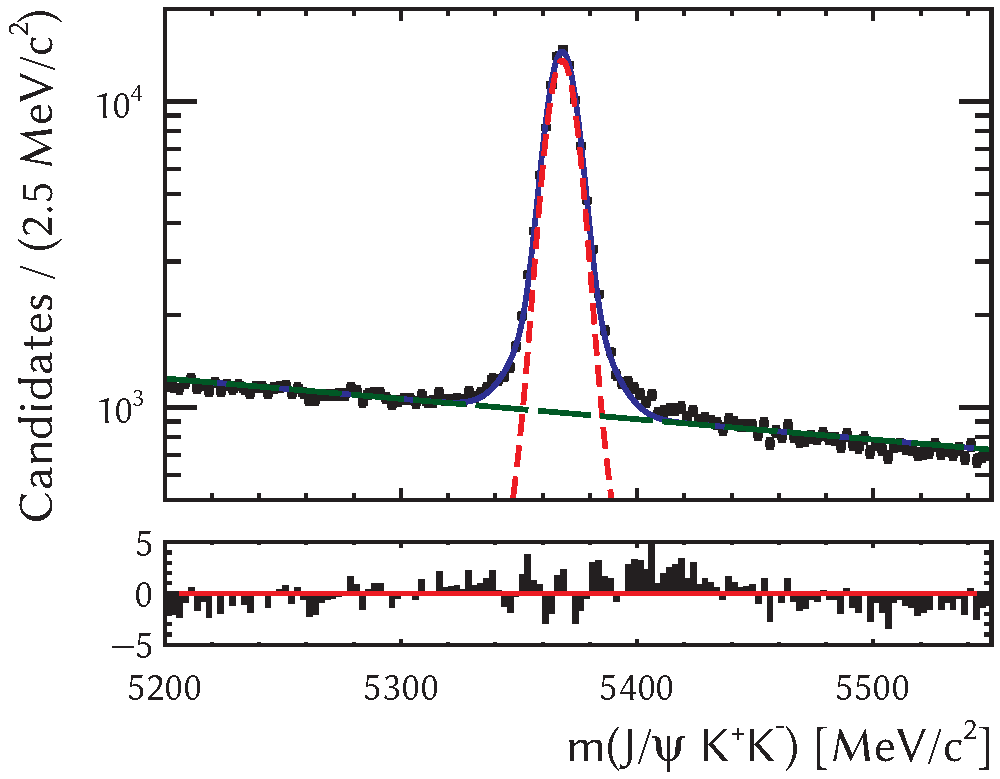
\includegraphics[width=\textwidth]{graphics/analysis/JpsiKKMass_DG_log_resid}
    \caption{}
    \label{fig:JpsiKKMass_DG_log}
  \end{subfigure}%
  \caption{Distribution of \BstoJpsiKK{} decay candidates in $\JpsiKK$ mass in
           (a) the signal mass range and
           (b) the full mass range on a logarithmic vertical scale.
           The black points show the distribution of the data and the blue, solid line shows a model that was fitted to the data.
           The model is the sum of two Gaussian shapes for the signal (shown by the red, short-dashed line)
           and an exponential shape for combinatorial background (shown by the green, long-dashed line).}
  \label{fig:JpsiKKMass_DG}
\end{figure}

In the areas below the $\JpsiKK$-mass distributions in Figure~\ref{fig:JpsiKKMass_DG} the corresponding \emph{residuals} are shown for each
mass bin. The residual is defined as the difference in values for the data and the (average) PDF in the bin, divided by the statistical
uncertainty of the data value. It is randomly distributed and quantifies how well the model describes the data in each bin. The residuals
in Figure~\ref{fig:JpsiKKMass_DG_log} seem to indicate a problem with the mass model, since the PDF generally underestimates the number of
decay candidates in the region of the signal peak, while it overestimates the number of candidates at the edges of the mass range. This
issue is mainly caused by misidentified backgrounds and will be addressed in Section~\ref{subsec:ana_bkgSub_bkgSub}.

Notice from Figures~\ref{fig:JpsiKKMassSel} and \ref{fig:JpsiKKMass_DG} that the signal candidates are concentrated in a mass window of
approximately 60\unitsp\MeV, centred at the $\Bs$ mass, where the signal fraction is approximately 80\%. The regions to the left and the
right of this \emph{signal window} are called mass \emph{side bands} and contain mainly background candidates. The candidates in the side
bands are used to estimate the time and angular distribution of the combinatorial background and subtract this from the total distribution
in the signal window to obtain the signal distribution. This procedure is described in the following section.


%%%%%%%%%%%%%%%%%%%%%%%%%%%%%%%%%%%
\subsection{Background Subtraction}
\label{subsec:ana_bkgSub_bkgSub}
%%%%%%%%%%%%%%%%%%%%%%%%%%%%%%%%%%%

The distribution of background decay candidates that remain after selection is subtracted from the total distribution by including
background candidates with negative weights in the data sample. For combinatorial background the most straightforward method of doing this
would be to give candidates in the signal region a weight equal to plus one and candidates in the $\JpsiKK$-mass side bands a small
negative weight, such that the contributions of background in the signal and side-band regions exactly cancel. Note that this assumes that
the background distribution in all variables of interest does not depend on the $\JpsiKK$ mass.

Because the definitions of the signal and side-band regions are rather arbitrary, a more sophisticated technique is applied. Although the
bulk of the signal decay candidates have a reconstructed $\JpsiKK$ mass in a region of approximately 60\unitsp\MeV{} around the $\Bs$ mass,
the tails of the signal mass distribution stretch beyond this mass window. Moreover, at the edges of the signal window the contribution of
background is larger than in the centre. To take these features of the mass distribution into account and estimate the contribution of
combinatorial background in the most optimal way, the candidate weights are not binary, but take a different value at each point in
$\JpsiKK$ mass.

The weights for subtracting combinatorial background are computed with the \splot/\sfit{} technique~\cite{Pivk:2004ty,*Xie:2009rka}, which
takes the $\JpsiKK$-mass distributions of the signal and the background as inputs. The resulting candidate weights are called
\emph{\sweight[s]}, which are larger than one in the centre of the signal peak and gradually become smaller away from the peak until they
are negative in the side bands.

The \splot/\sfit{} method assumes that, in addition to the background distribution, also the signal distribution in the variables of
interest does not depend on the $\JpsiKK$ mass. In other words, there can be no correlations between the $\JpsiKK$ mass and any other
variable that is to be analysed, for both the signal and the background distribution (but not their sum).

Before fitting the distribution of signal and combinatorial-background candidates and computing \sweight[s], the contributions from other
backgrounds are subtracted by adding decay candidates with negative weights to the data sample. Two additional backgrounds are considered,
both originating from the misidentification of particles in the detector: \BdtoJpsiKstKpi{} and \LbtoJpsipK. Because the detected particles
for these processes originate from decays of unstable particles (resonances), these contributions are also called \emph{resonant
backgrounds}.

\begin{figure}[tb]
  \centering
  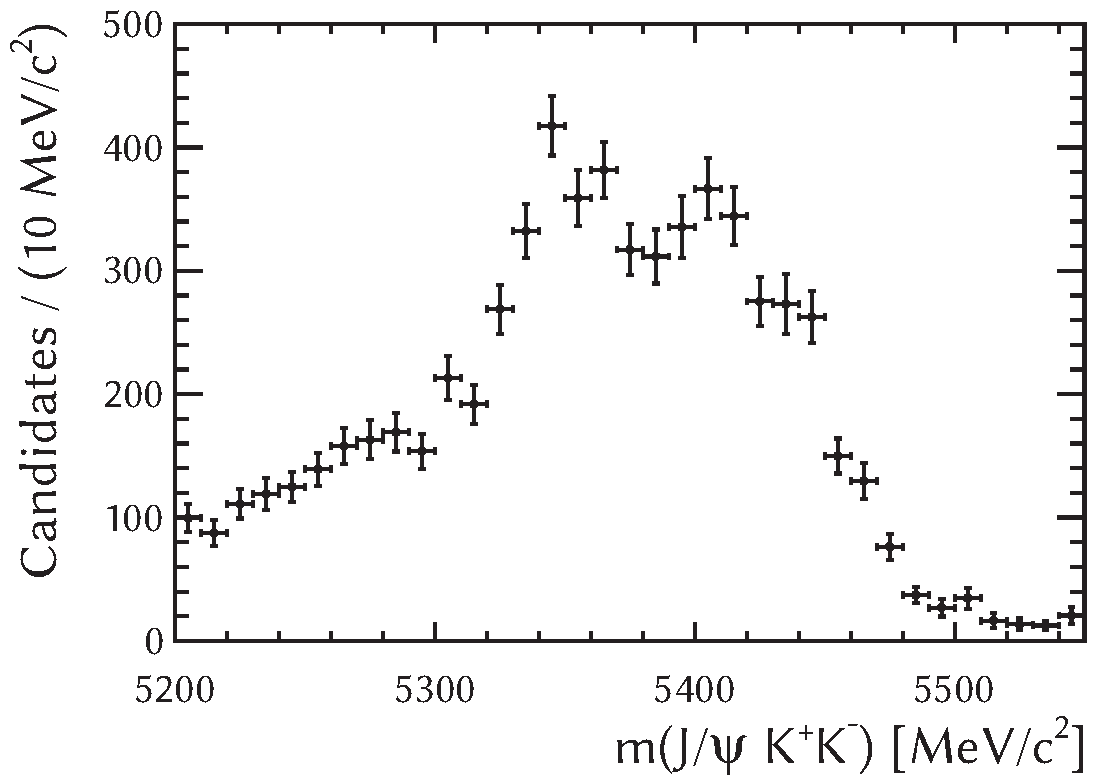
\includegraphics[width=0.5\textwidth]{graphics/analysis/JpsiKKMass_peakBkg}
  \caption{Distribution of weighted simulated resonant-background \BstoJpsiKK{} decay candidates in $\JpsiKK$ mass in the full mass range.}
  \label{fig:JpsiKKMass_peakBkg}
\end{figure}

Figure~\ref{fig:JpsiKKMass_peakBkg} shows the sum of the reconstructed $\JpsiKK$-mass distributions for the two resonant backgrounds. They
form a broad structure, without features that clearly distinguish these backgrounds from the signal and from combinatorial background.
Therefore, the resonant backgrounds are subtracted by adding simulated \BdtoJpsiKstKpi{} and \LbtoJpsipK{} decay candidates to the data
sample with negative weights that represent the amount of real resonant-background data, in total approximately seven thousand candidates.
Uncertainties in the numbers of background candidates and their distributions lead to systematic uncertainties in the final parameter
estimates, as will be discussed in Section~\ref{sec:result_syst}.

The $\JpsiKK$-mass distribution after subtracting the two resonant backgrounds is shown in Figure~\ref{fig:JpsiKKMass_DG_bkgSub}. Comparing
to Figure~\ref{fig:JpsiKKMass_DG}, it can be seen from the residuals that the PDF follows the data more closely. The systematic
underestimates of the numbers of decay candidates in the signal region and the overestimates in the side-band regions have reduced. It
appears, however, that this effect is still partially present. Moreover, the residuals in the signal region seem to be large than one would
expect.

\begin{figure}[tbp]
  \centering
  \begin{subfigure}{0.49\textwidth}
    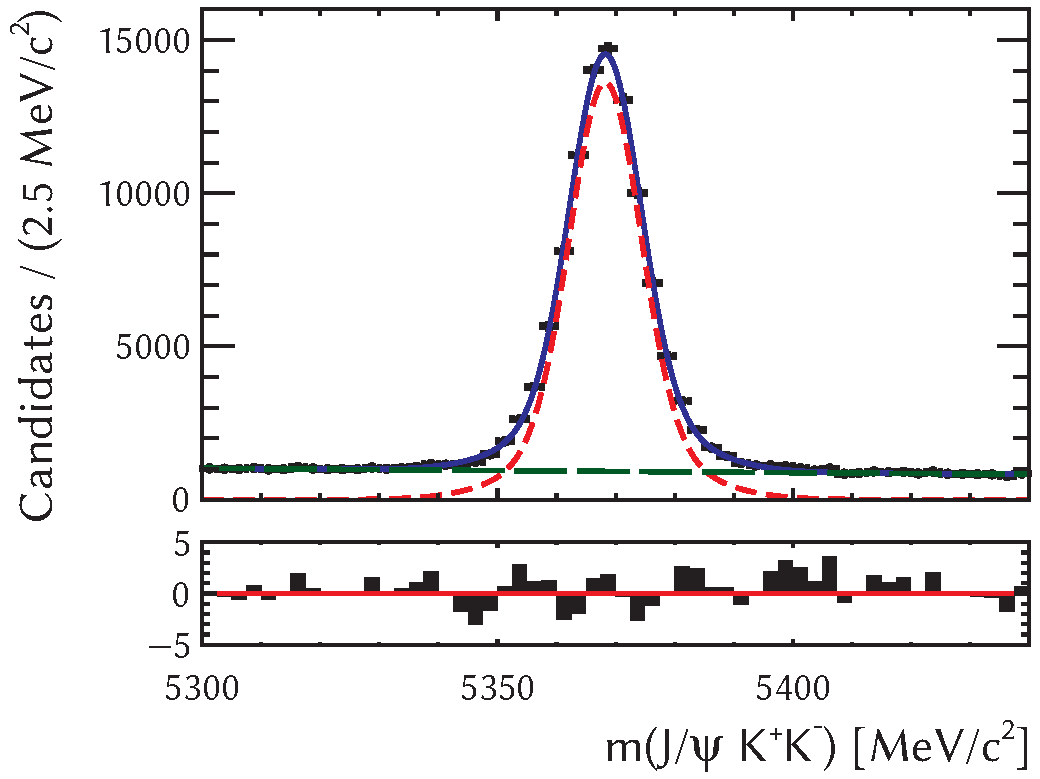
\includegraphics[width=\textwidth]{graphics/analysis/JpsiKKMass_DG_bkgSub_lin_resid}
    \caption{}
    \label{fig:JpsiKKMass_I2_lin}
  \end{subfigure}%
  \hfill%
  \begin{subfigure}{0.49\textwidth}
    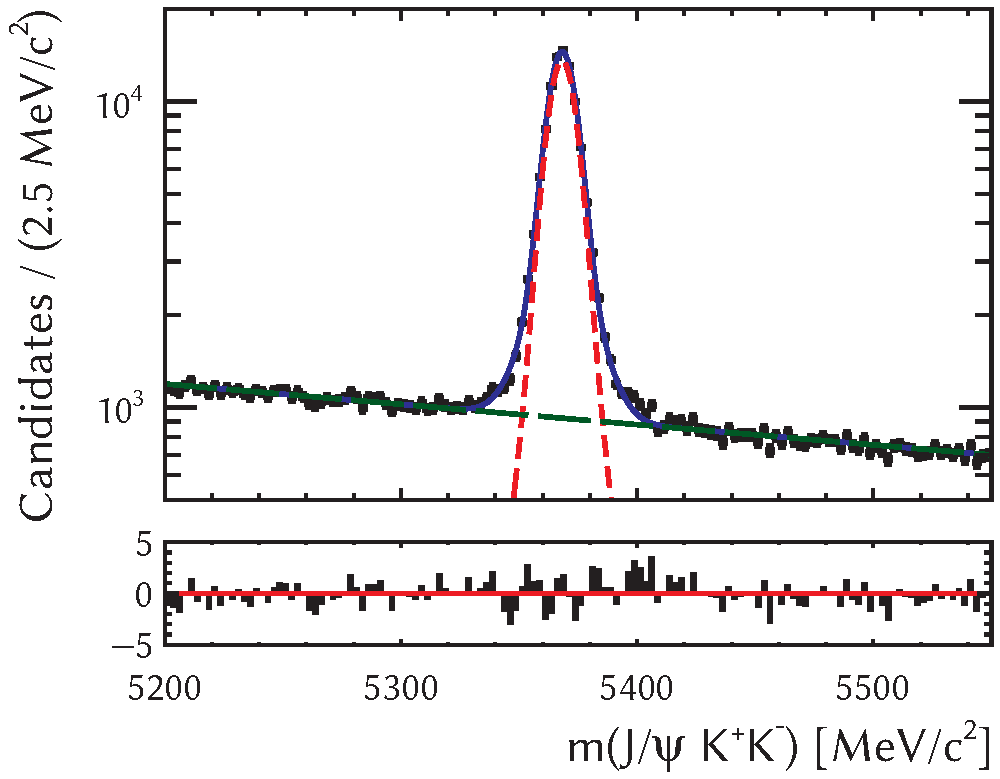
\includegraphics[width=\textwidth]{graphics/analysis/JpsiKKMass_DG_bkgSub_log_resid}
    \caption{}
    \label{fig:JpsiKKMass_I2_log}
  \end{subfigure}%
  \caption{Distribution of \BstoJpsiKK{} decay candidates in $\JpsiKK$ mass after subtracting resonant backgrounds in
           (a) the signal mass range and
           (b) the full mass range on a logarithmic vertical scale.
           The black points show the distribution of the data and the blue, solid line shows a model that was fitted to the data.
           The model is the sum of two Gaussian shapes for the signal (shown by the red, short-dashed line)
           and an exponential shape for combinatorial background (shown by the green, long-dashed line).}
  \label{fig:JpsiKKMass_DG_bkgSub}
\end{figure}

\begin{figure}[tbp]
  \centering
  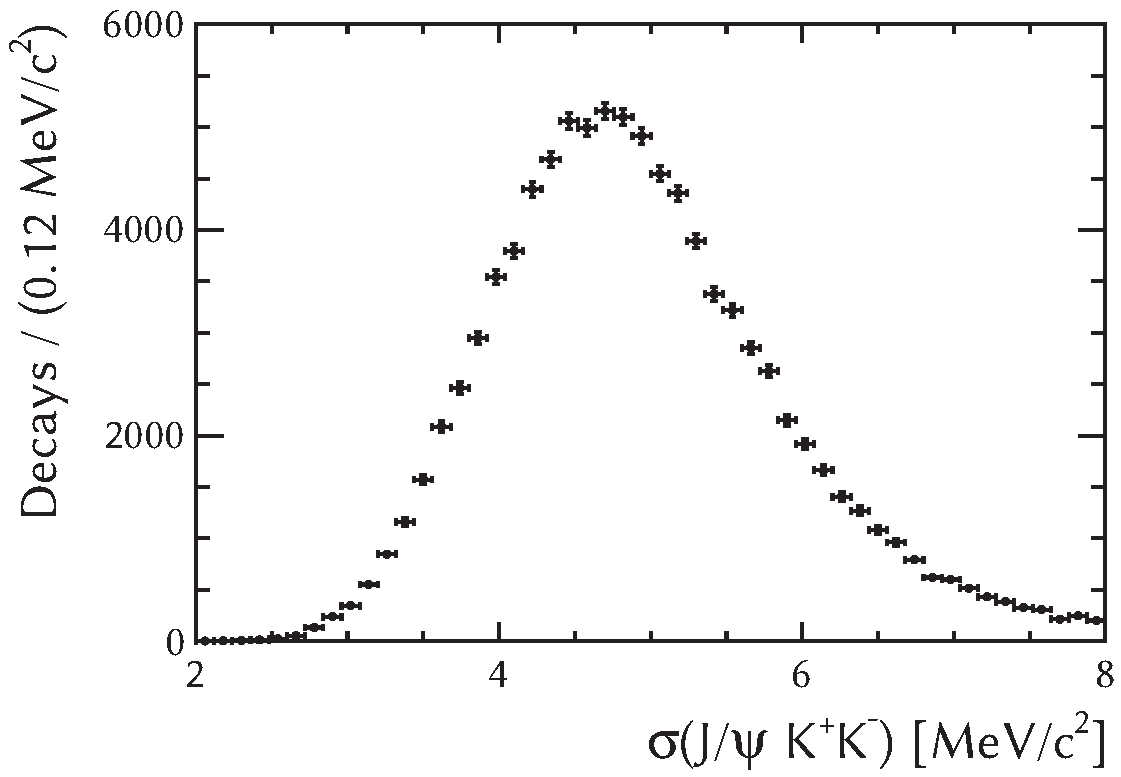
\includegraphics[width=0.5\textwidth]{graphics/analysis/JpsiKKMassErr}
  \caption{Distribution of \BstoJpsiKK{} signal decays in the estimated $\JpsiKK$-mass uncertainty.}
  \label{fig:JpsiKKMassErr}
\end{figure}

To address these issues, the double-Gaussian signal model is replaced by a more sophisticated model for the mass resolution.
Figure~\ref{fig:JpsiKKMassErr} shows the distribution of the estimated uncertainty in the $\JpsiKK$-mass measurement for each decay. This
distribution does not feature a structure with two sharp peaks, as would be expected for a double-Gaussian mass model, but is instead described
by one broad peak. To describe the resulting mass distribution a double-sided Hypatia function with a symmetric core~\cite{Santos:2013gra} is
used, which is designed to describe the effects of an experimental resolution that is different for each decay candidate.

The Hypatia function is defined by
\begin{subequations}
\begin{equation}
  I(m) \equiv
  \begin{cases}
    \left[(m-\mu)^{2} + \delta^{2}\right]^{\frac{1}{2} \lambda - \frac{1}{4}}
          \!\!\!\!& K_{\lambda - \frac{1}{2}}\big(\alpha \sqrt{(m-\mu)^2 + \delta^2}\big) \\
          &\text{if}\ \ -a_L\,\sigma < m - \mu < +a_R\,\sigma \\
    \frac{A_L}{(B_L - m+\mu)^{n_L}} &\text{if}\ \ m - \mu < -a_L\,\sigma \\
    \frac{A_R}{(B_R + m-\mu)^{n_R}} &\text{if}\ \ m - \mu > +a_R\,\sigma
  \end{cases}
\end{equation}
with
\begin{equation}
  \alpha\equiv\frac{1}{\sigma}\sqrt{\frac{\zeta\, K_{\lambda+1}(\zeta)}{K_\lambda(\zeta)}}
  \qquad\text{and}\qquad
  \delta\equiv\sigma\sqrt{\frac{\zeta\,K_\lambda(\zeta)}{K_{\lambda+1}(\zeta)}} \ ,
\end{equation}
\end{subequations}
where $m$ is the mass variable and $K_{\nu}(z)$ the modified Bessel function of the second kind. The parameter $\mu$ controls the position
of the mass peak, $\sigma$ controls the width of its core, and $\lambda$ and $\zeta$ control the shape of its core. The double-sided
Hypatia function has an enhanced tail on both the left and the right side of the mass peak, the positions and shapes of which are
controlled by the parameters $a_{L/R}$ and $n_{L/R}$, respectively. The parameters $A_{L/R}$ and $B_{L/R}$ are obtained by imposing
continuity and differentiability at the points of transition between the core of the function and its tails.

The Hypatia parameters $\lambda$\textapprox\tm2.5, 0\textlt$\zeta$\textlt0.5, $a_{L/R}$\textapprox2.5, and 0\textlt$n_{L/R}$\textlt3 are
determined from simulated \BstoJpsiphi{} signal decays. Only the mean ($\mu$\textapprox5368\unitsp\MeV) and the width
($\sigma$\textapprox8\unitsp\MeV) of the core are determined in a fit to the real data. Consequently, the number of free parameters in the
Hypatia model is smaller than in the double-Gaussian model, for which the mean, the two widths, and the relative contribution of the two
functions were free parameters.

The result of a fit with the Hypatia signal model and an exponential shape for the combinatorial background is shown in
Figure~\ref{fig:JpsiKKMass_I2_bkgSub}. The improvement with the Hypatia model can be seen from the residuals, which have become smaller in
the signal region and are more symmetrically distributed around zero in comparison to Figure~\ref{fig:JpsiKKMass_DG_bkgSub}.

\begin{figure}[tbp]
  \centering
  \begin{subfigure}{0.49\textwidth}
    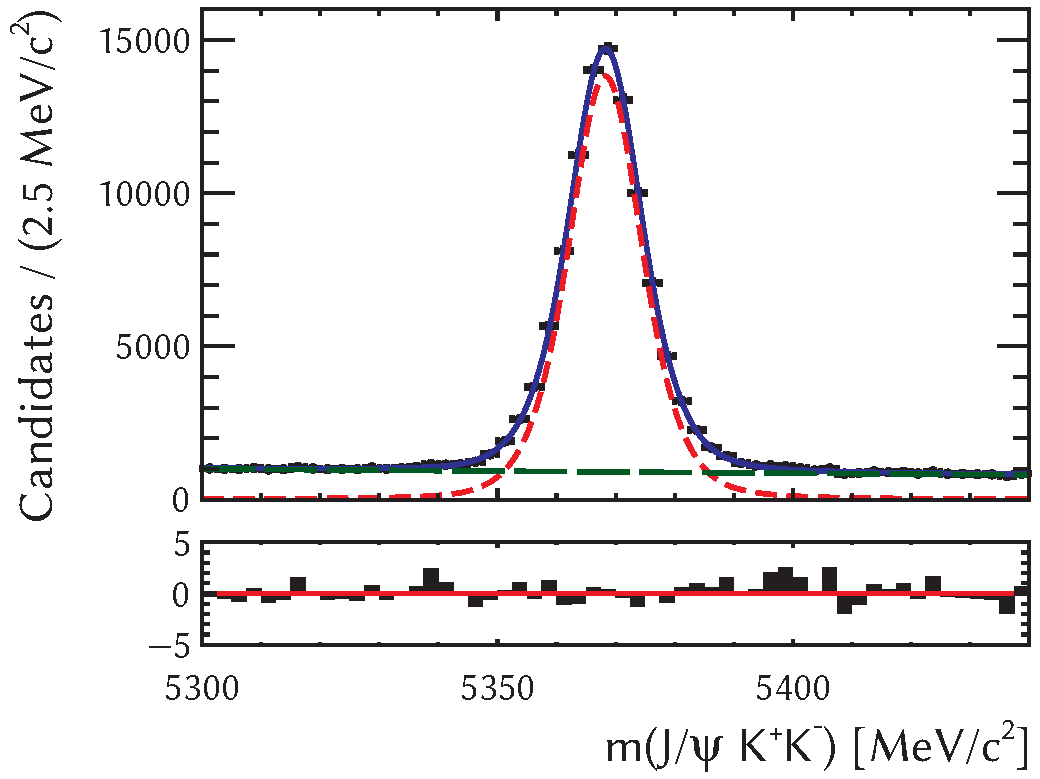
\includegraphics[width=\textwidth]{graphics/analysis/JpsiKKMass_I2_bkgSub_lin_resid}
    \caption{}
    \label{fig:JpsiKKMass_I2_bkgSub_lin}
  \end{subfigure}%
  \hfill%
  \begin{subfigure}{0.49\textwidth}
    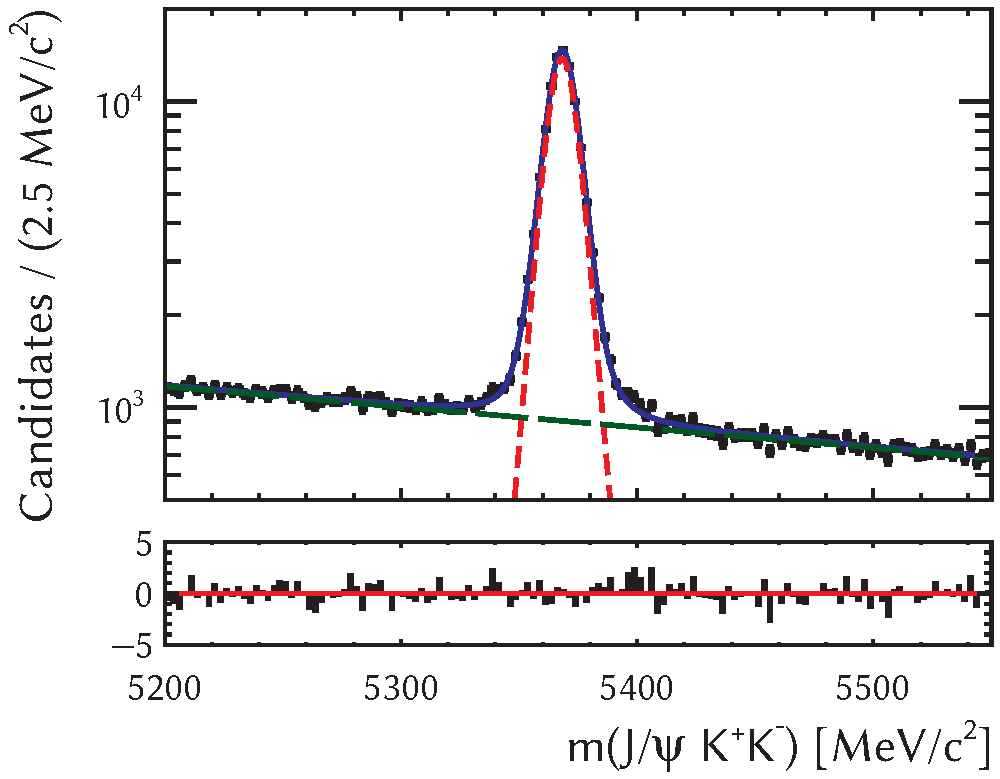
\includegraphics[width=\textwidth]{graphics/analysis/JpsiKKMass_I2_bkgSub_log_resid}
    \caption{}
    \label{fig:JpsiKKMass_I2_bkgSub_log}
  \end{subfigure}%
  \caption{Distribution of \BstoJpsiKK{} decay candidates in $\JpsiKK$ mass after subtracting resonant backgrounds in
           (a) the signal mass range and
           (b) the full mass range on a logarithmic vertical scale.
           The black points show the distribution of the data and the blue, solid line shows a model that was fitted to the data.
           The model is the sum of an Hypatia shape for the signal (shown by the red, short-dashed line)
           and an exponential shape for combinatorial background (shown by the green, long-dashed line).}
  \label{fig:JpsiKKMass_I2_bkgSub}
\end{figure}

Studies of the $\JpsiKK$-mass shape of signal decays have shown that it depends on the $\KK$ invariant mass. Therefore, the parameters of
the mass model are determined separately in the $\KK$-mass bins that are also used in the final time and angular model to determine the
trend in the difference between the $\Jpsiphi$ and $\KK$ S-wave phases (see Section~\ref{subsec:pheno_equations_symmetry}). Combinatorial
background is subtracted separately for each bin.

The $\KK$-mass bins are defined in Table~\ref{tab:KKBins}. In addition to the binning, the table also lists the final numbers of signal and
combinatorial-background decays and the weighted-likelihood correction factors (see Section~\ref{subsec:ana_fit_weights}) for each bin.

\begin{table}[p]
  \centering
  \caption{Definition of the bins in $\KK$ invariant mass.}
  \label{tab:KKBins}
  \begin{tabular}{cccccc}
    \hline
    bin  &  range [\MeV]          &  signal [\tenpow{3}]  &  comb. bkg. [\tenpow{3}]  &  $\alpha_{2011}$  &  $\alpha_{2012}$  \\
    \hline
    1    &  \phantom{0}990--1008  &  \phantom{0}2         &  23                          &  0.42          &  0.39             \\
    2    &  1008--1016            &  10                   &  15                          &  0.79          &  0.76             \\
    3    &  1016--1020            &  35                   &  11                          &  0.94          &  0.93             \\
    4    &  1020--1024            &  28                   &  12                          &  0.92          &  0.92             \\
    5    &  1024--1032            &  13                   &  19                          &  0.77          &  0.77             \\
    6    &  1032--1050            &  \phantom{0}8         &  46                          &  0.51          &  0.51             \\
    \hline
  \end{tabular}
\end{table}

\begin{table}[p]
  \centering
  \caption{Parameters of the $\JpsiKK$-mass model that is used for background subtraction.}
  \label{tab:JpsiKKMassPars}
  \begin{tabular}{ccc}
    \hline
    par.                      &  value            &  stat. uncert.  \\
                              &  [\MeV]           &  [\MeV]         \\
    \hline
    $\mu_1$                   &  5368.47          &  0.25           \\
    $\mu_2$                   &  5367.79          &  0.09           \\
    $\mu_3$                   &  5367.93          &  0.04           \\
    $\mu_4$                   &  5368.65          &  0.05           \\
    $\mu_5$                   &  5368.69          &  0.08           \\
    $\mu_6$                   &  5368.39          &  0.13           \\
    $\sigma_{1,\mathrm{b}}$   &  \phantom{0}8.9   &  0.4            \\
    $\sigma_{2,\mathrm{b}}$   &  \phantom{0}8.23  &  0.11           \\
    $\sigma_{3,\mathrm{b}}$   &  \phantom{0}7.98  &  0.05           \\
    $\sigma_{4,\mathrm{b}}$   &  \phantom{0}7.87  &  0.05           \\
    $\sigma_{5,\mathrm{b}}$   &  \phantom{0}8.40  &  0.10           \\
    $\sigma_{6,\mathrm{b}}$   &  \phantom{0}8.90  &  0.18           \\
    $\sigma_{1,\mathrm{nb}}$  &  14.7             &  3.4            \\
    $\sigma_{2,\mathrm{nb}}$  &  \phantom{0}6.2   &  0.9            \\
    $\sigma_{3,\mathrm{nb}}$  &  \phantom{0}7.0   &  0.4            \\
    $\sigma_{4,\mathrm{nb}}$  &  \phantom{0}7.0   &  0.5            \\
    $\sigma_{5,\mathrm{nb}}$  &  \phantom{0}7.1   &  0.9            \\
    $\sigma_{6,\mathrm{nb}}$  &  \phantom{0}7.6   &  1.8            \\
    \hline
  \end{tabular}%
  \hspace*{15pt}%
  \begin{tabular}{ccc}
    \hline
    par.                         &  value            &  stat. uncert.  \\
     &  [$c$\textsuperscript{2}/MeV]  &  [$c$\textsuperscript{2}/MeV]  \\
    \hline
    $\gamma_{\mathrm{b},2011}$   &  0.00176  &  0.00006  \\
    $\gamma_{\mathrm{b},2012}$   &  0.00153  &  0.00003  \\
    $\gamma_{\mathrm{nb},2011}$  &  0.00032  &  0.00024  \\
    $\gamma_{\mathrm{nb},2012}$  &  0.00054  &  0.00015  \\
    \hline
    & & \\ & & \\ & & \\ & & \\ & & \\ & & \\ & & \\ & & \\ & & \\ & & \\ & & \\ & & \\ & & \\ & & \\
  \end{tabular}
\end{table}

There is no evidence for the $\JpsiKK$-mass distribution of the background to depend on the $\KK$ mass, but it does depend on two other
variables in the data. The background distribution is found to be different for the 2011 and 2012 run periods and for decay candidates that
are selected by the biased HLT2 trigger and candidates that are exclusively selected by the unbiased HLT2 trigger. Because these two
variables are used in the measurement and implementation of the decay-time efficiency function (see Section~\ref{subsec:ana_time_acc}),
background subtraction is also performed separately in the four categories associated to these variables. In addition, the  width of the
signal peak is determined separately for HLT2-biased and not-HLT2-biased candidates.

The final parameters of the $\JpsiKK$-mass model that were determined from the real data are listed in Table~\ref{tab:JpsiKKMassPars},
where the exponential function for the background mass distribution is described by $e^{-\gamma m}$. The number of signal decays determined
with this model is 96 thousand and the number of combinatorial-background decays 127 thousand.

To check if the decay time and angles are not correlated with the $\JpsiKK$ mass, the mass distribution is plotted for different bins in
time and angles. A problem appears in $\cthetal$, for which the mass distributions are shown in the bins $|\cthetal|$\textlt0.25,
0.25\textle$|\cthetal|$\textlt0.7, and $|\cthetal|$\textge0.7 in Figure~\ref{fig:JpsiKKMass_I2_bkgSub_ctl}. In all three cases the nominal
mass model from Figure~\ref{fig:JpsiKKMass_I2_bkgSub} is shown.
\begin{figure}[tbp]
  \centering
  \begin{subfigure}{0.49\textwidth}
    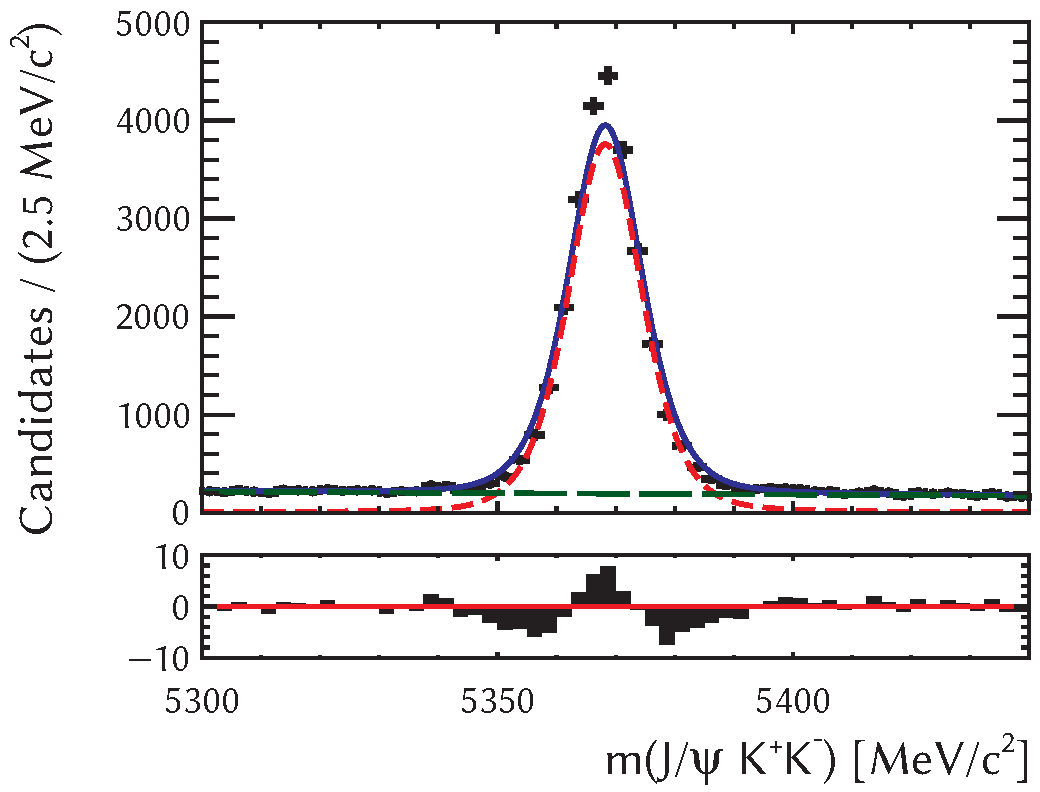
\includegraphics[width=\textwidth]{graphics/analysis/JpsiKKMass_I2_bkgSub_ctl2_lin_resid}
    \caption{}
    \label{fig:JpsiKKMass_I2_bkgSub_ctl2_lin}
  \end{subfigure}%
  \hfill%
  \begin{subfigure}{0.49\textwidth}
    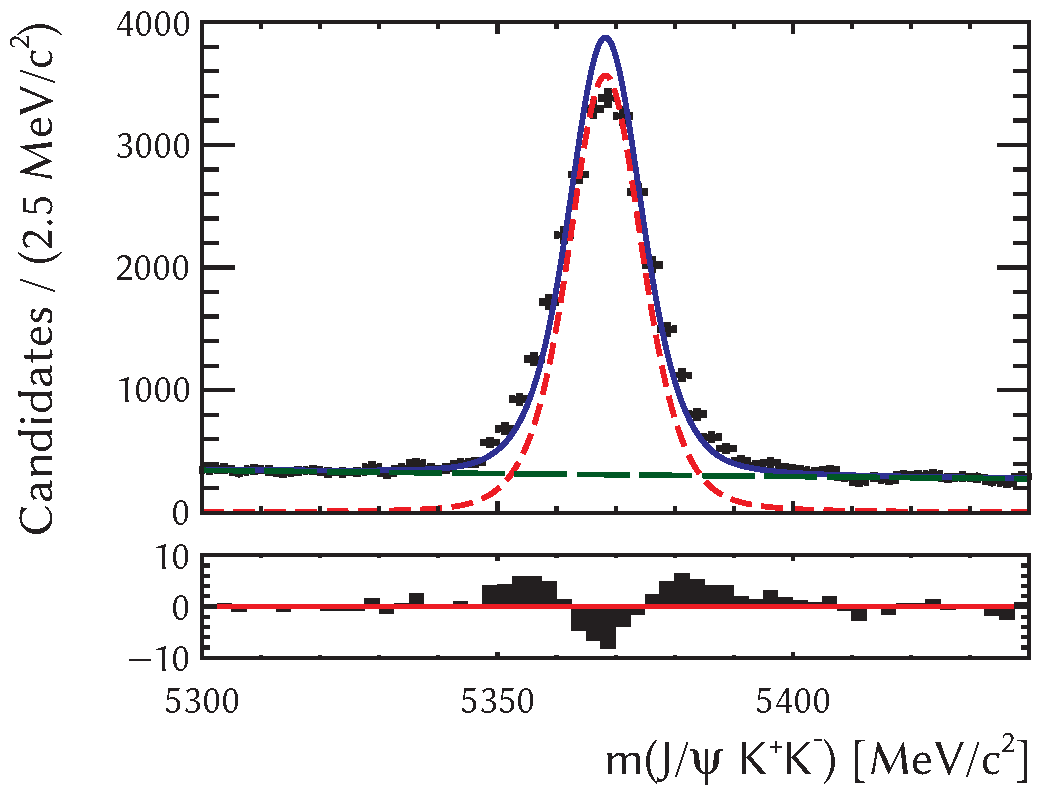
\includegraphics[width=\textwidth]{graphics/analysis/JpsiKKMass_I2_bkgSub_ctl04_lin_resid}
    \caption{}
    \label{fig:JpsiKKMass_I2_bkgSub_ctl04_lin}
  \end{subfigure}

  \vspace*{0.02\textwidth}
  \begin{subfigure}{0.49\textwidth}
    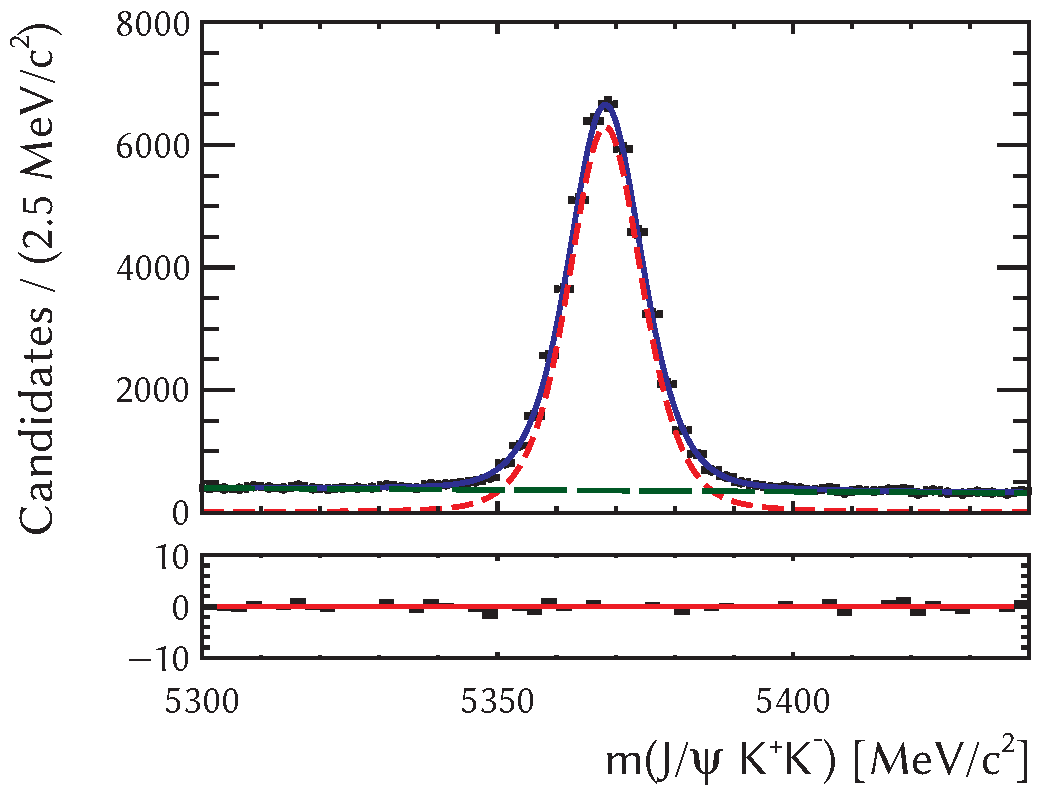
\includegraphics[width=\textwidth]{graphics/analysis/JpsiKKMass_I2_bkgSub_ctl13_lin_resid}
    \caption{}
    \label{fig:JpsiKKMass_I2_bkgSub_ctl13}
  \end{subfigure}%
  \caption{Distribution of \BstoJpsiKK{} decay candidates in $\JpsiKK$ mass after subtracting resonant backgrounds in bins of $\cthetal$,
           where the shape of the model is set to the nominal shape from Figure~\ref{fig:JpsiKKMass_I2_bkgSub}.
           (a) $|\cthetal|$\textlt0.25,
           (b) $|\cthetal|$\textge0.7,
           (c) 0.25\textle$|\cthetal|$\textlt0.7.}
  \label{fig:JpsiKKMass_I2_bkgSub_ctl}
\end{figure}

\begin{figure}[tbp]
  \centering
  \begin{subfigure}{0.49\textwidth}
    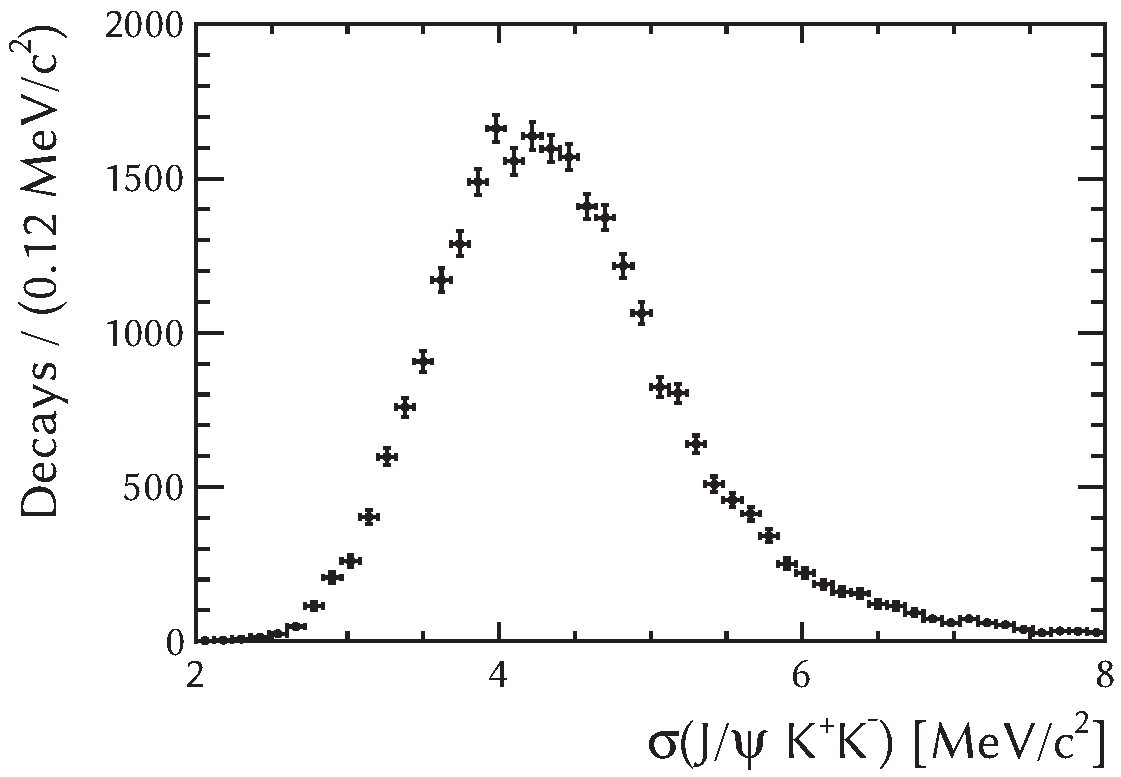
\includegraphics[width=\textwidth]{graphics/analysis/JpsiKKMassErr_left}
    \caption{}
    \label{fig:JpsiKKMassErr_left}
  \end{subfigure}%
  \hfill%
  \begin{subfigure}{0.49\textwidth}
    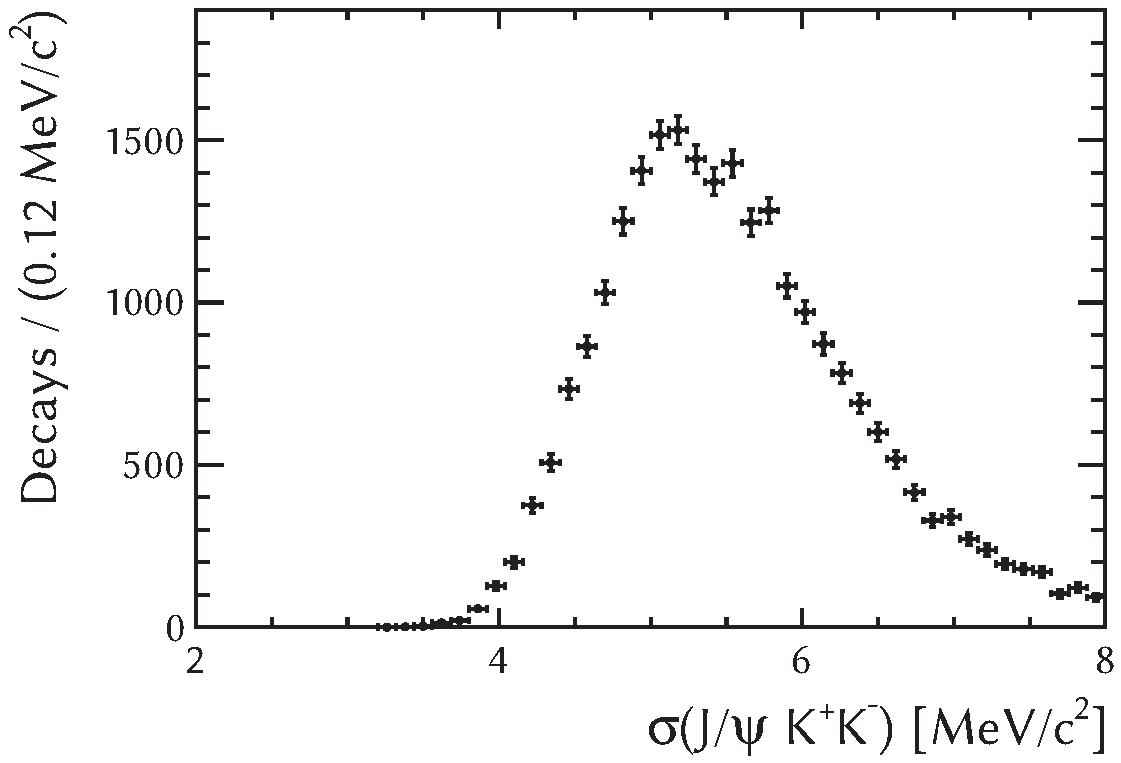
\includegraphics[width=\textwidth]{graphics/analysis/JpsiKKMassErr_right}
    \caption{}
    \label{fig:JpsiKKMassErr_right}
  \end{subfigure}

  \vspace*{0.02\textwidth}
  \begin{subfigure}{0.49\textwidth}
    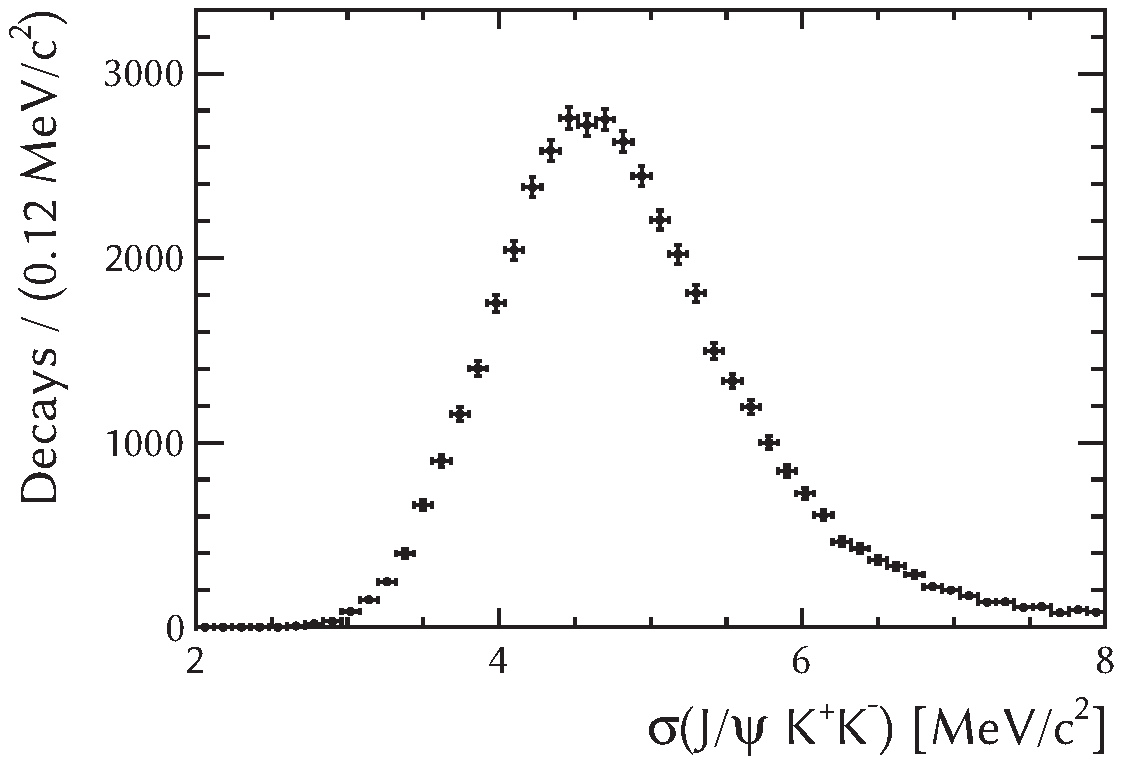
\includegraphics[width=\textwidth]{graphics/analysis/JpsiKKMassErr_middle}
    \caption{}
    \label{fig:JpsiKKMassErr_middle}
  \end{subfigure}%
  \caption{Distribution of \BstoJpsiKK{} signal decays in the estimated $\JpsiKK$-mass uncertainty in bins of $\cthetal$.
           (a) $|\cthetal|$\textlt0.25,
           (b) $|\cthetal|$\textge0.7,
           (c) 0.25\textle$|\cthetal|$\textlt0.7.}
  \label{fig:JpsiKKMassErr_ctlBins}
\end{figure}

\begin{figure}[p]
  \centering
  \begin{subfigure}{0.49\textwidth}
    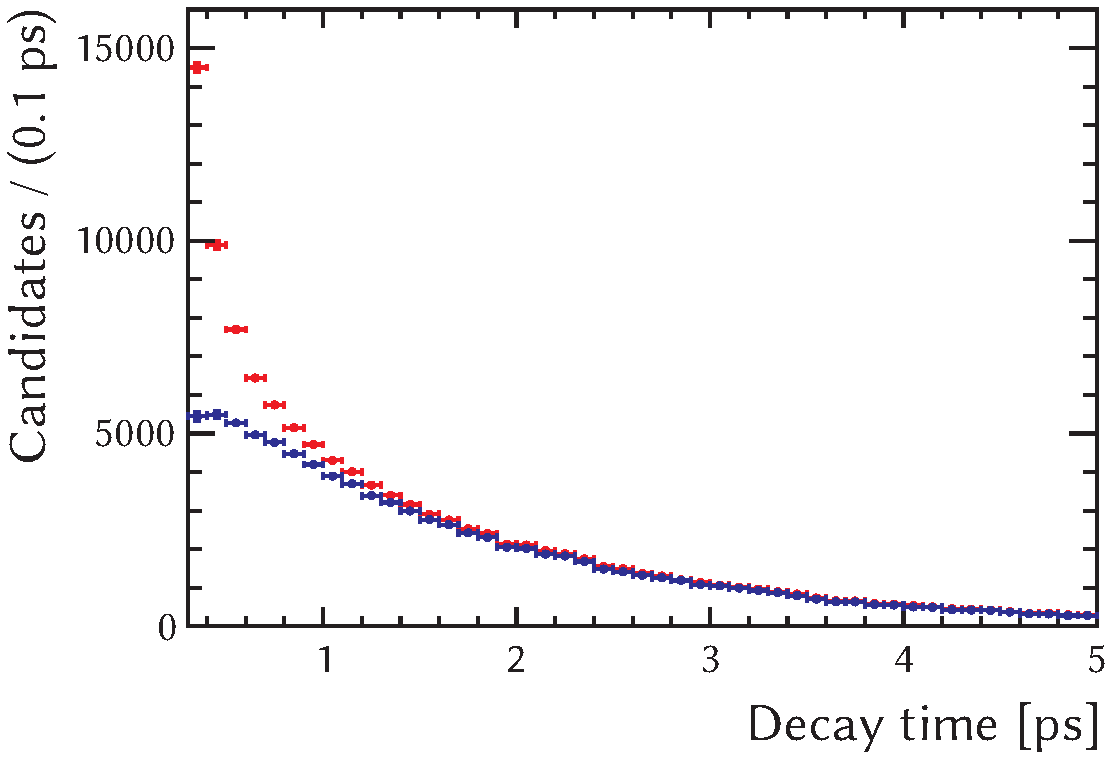
\includegraphics[width=\textwidth]{graphics/analysis/time_bkgSub}
    \caption{}
    \label{fig:timeBkgSub}
  \end{subfigure}%
  \hfill%
  \begin{subfigure}{0.49\textwidth}
    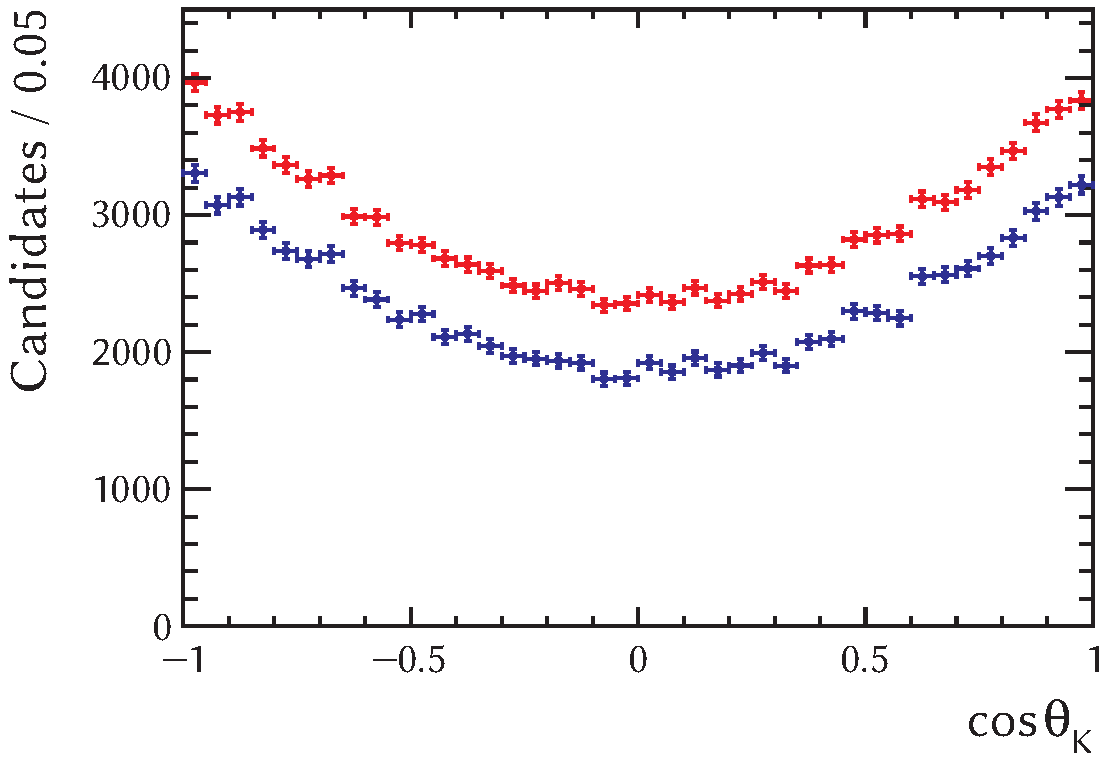
\includegraphics[width=\textwidth]{graphics/analysis/ctk_bkgSub}
    \caption{}
    \label{fig:ctkBkgSub}
  \end{subfigure}

  \vspace*{0.02\textwidth}
  \begin{subfigure}{0.49\textwidth}
    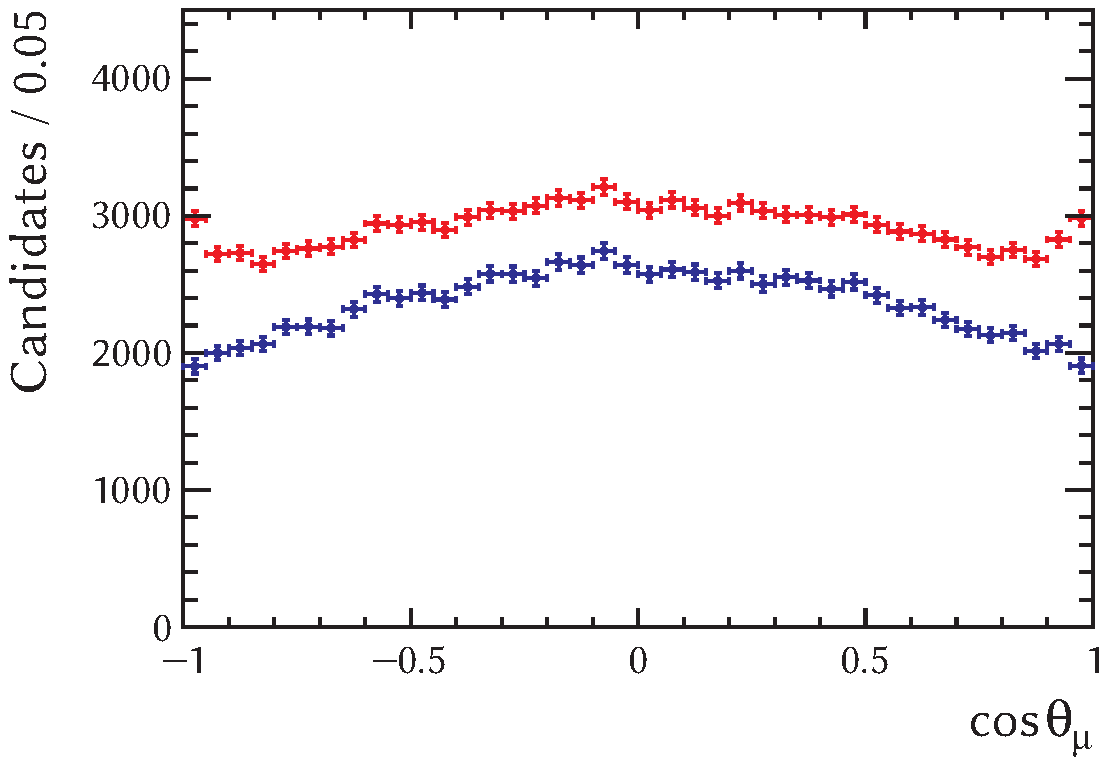
\includegraphics[width=\textwidth]{graphics/analysis/ctl_bkgSub}
    \caption{}
    \label{fig:ctlBkgSub}
  \end{subfigure}%
  \hfill%
  \begin{subfigure}{0.49\textwidth}
    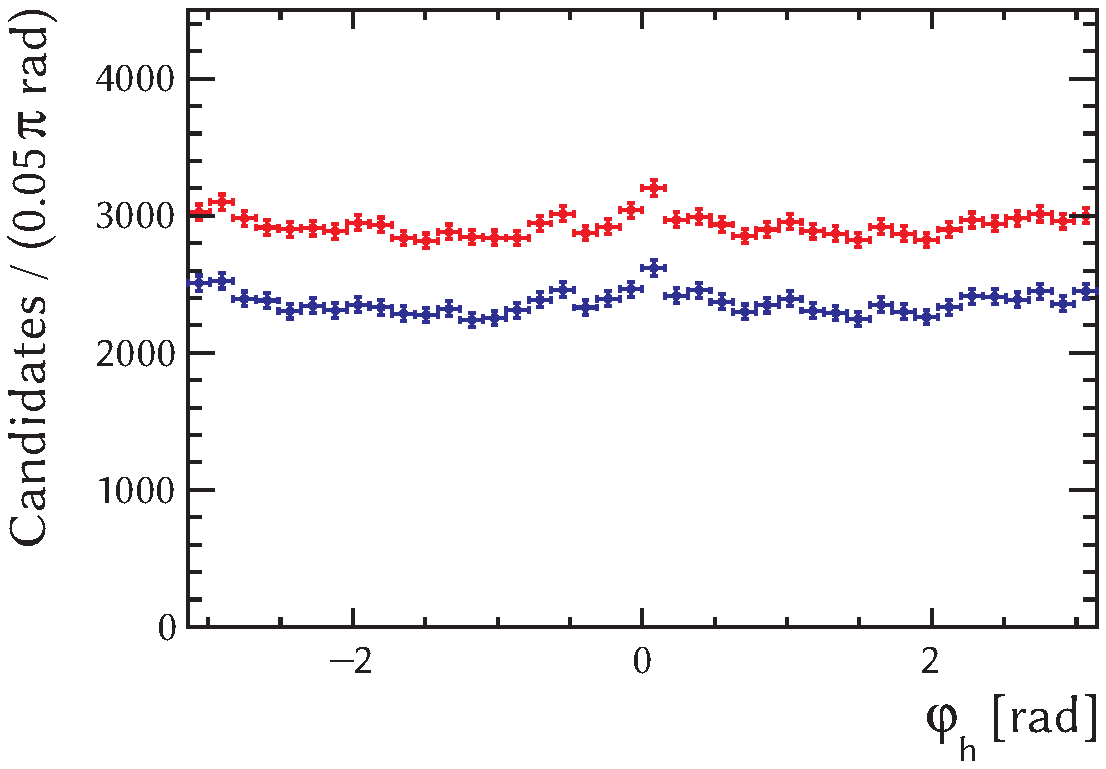
\includegraphics[width=\textwidth]{graphics/analysis/phi_bkgSub}
    \caption{}
    \label{fig:phiBkgSub}
  \end{subfigure}

  \vspace*{0.02\textwidth}
  \begin{subfigure}{0.49\textwidth}
    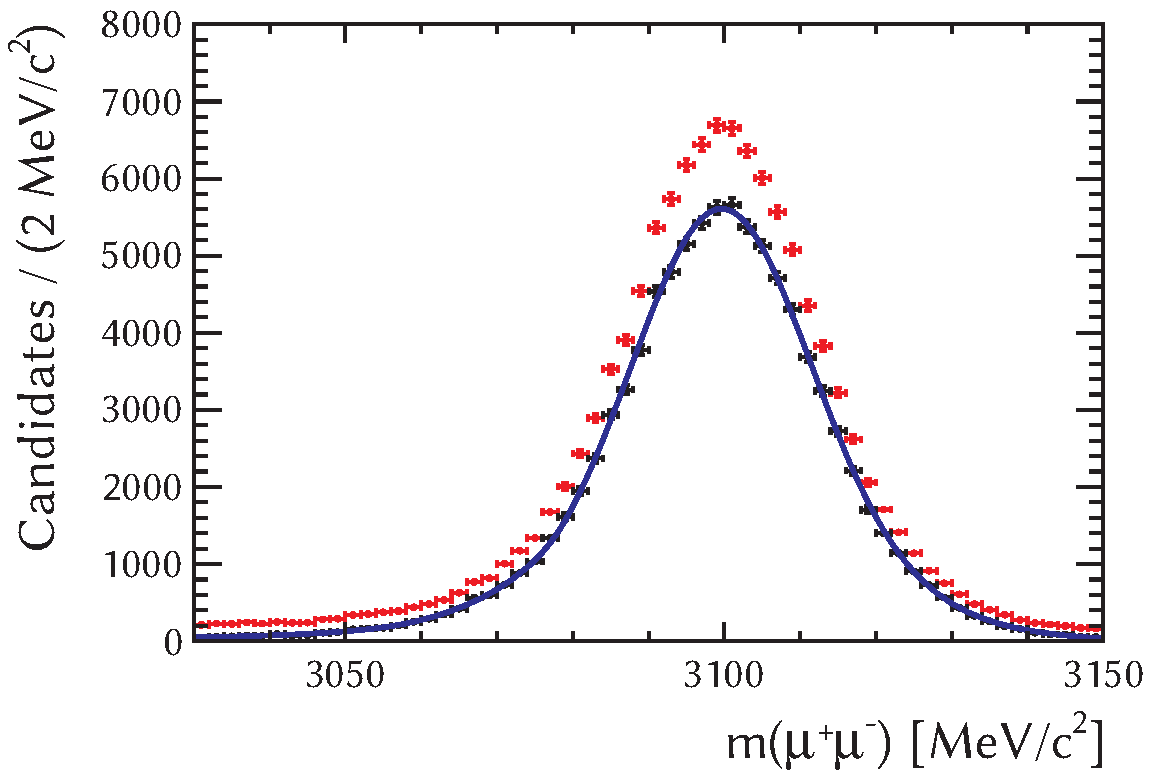
\includegraphics[width=\textwidth]{graphics/analysis/mumuMass_bkgSub_lin}
    \caption{}
    \label{fig:mumuMassBkgSub}
  \end{subfigure}%
  \hfill%
  \begin{subfigure}{0.49\textwidth}
    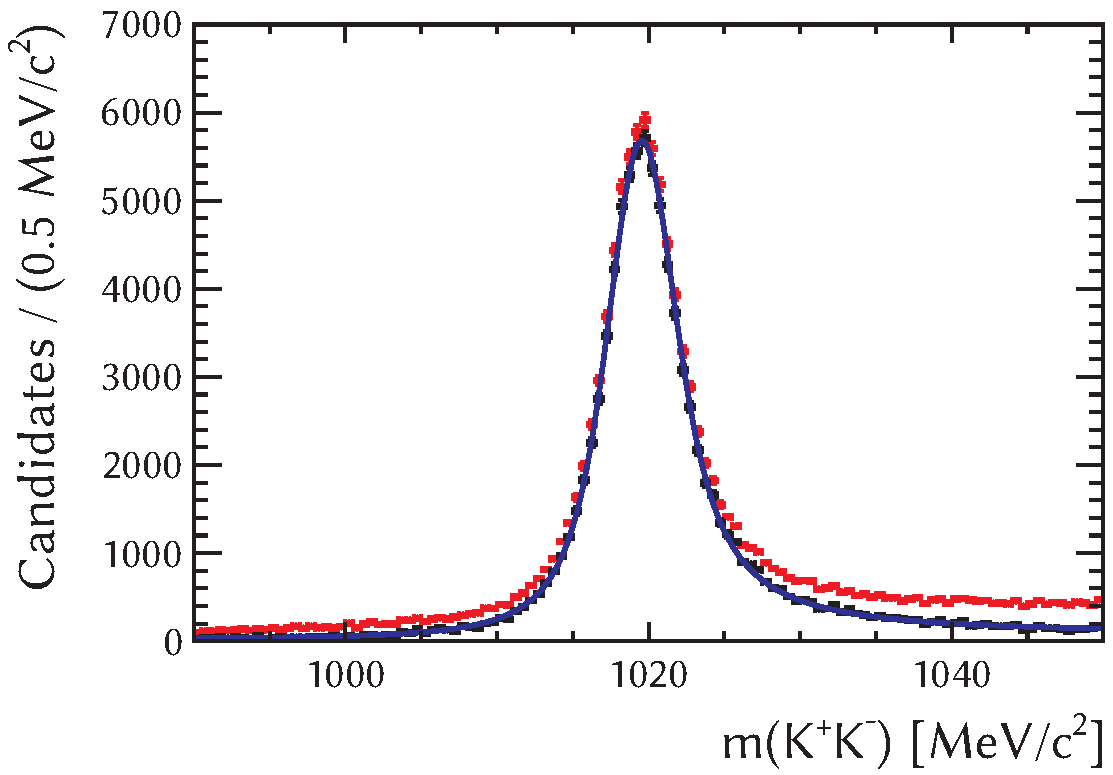
\includegraphics[width=\textwidth]{graphics/analysis/KKMass_bkgSub_lin}
    \caption{}
    \label{fig:KKMassBkgSub}
  \end{subfigure}%

  \caption{Distributions of \BstoJpsiKK{} decay candidates before (red) and after (blue) background subtraction
           in (a) decay time, (b) $\cthetaK$, (c) $\cthetal$, (d) $\phihel$, (e) $\mumu$ mass, and (f) $\KK$ mass.
           The distributions before background subtraction are for decay candidates
           in a $\JpsiKK$-mass window of 60\unitsp\MeV{} around the $\Bs$ mass.}
  \label{fig:obsBkgSub}
\end{figure}

From Figure~\ref{fig:JpsiKKMass_I2_bkgSub_ctl} it is clear that the $\JpsiKK$-mass resolution for the signal depends on the value of
$\cthetal$. This is also supported by Figure~\ref{fig:JpsiKKMassErr_ctlBins}, which shows that the distribution of the estimated $\JpsiKK$-mass
uncertainty varies for the three $\cthetal$ regions. Formally this means that the procedure of background subtraction does not work for the
$\cthetal$ distribution. The impact of this effect is studied by subtracting the background with the different mass models obtained in the
$\cthetal$ bins and a corresponding systematic uncertainty is evaluated (see Section~\ref{sec:result_syst}).

Figure~\ref{fig:obsBkgSub} shows the distributions of decay time, decay angles, $\mumu$ invariant mass, and $\KK$ invariant mass before and
after background subtraction. The distributions before background subtraction are only shown for a $\JpsiKK$-mass window of 60\unitsp\MeV{}
around the $\Bs$ mass.

From the decay-time distribution in Figure~\ref{fig:timeBkgSub} it can be seen that most background candidates have a small decay time.
Notice that the decay-time range in this plot starts at 0.3\unitsp{}ps. Even though the first of the oscillations in the decay time
distribution of the signal is lost, this requirement improves the measurement, because it removes a significant amount of background, as
shown in Section~\ref{subsec:ana_bkgSub_sel}.

The model that was fitted to the $\mumu$-mass distribution in Figure~\ref{fig:mumuMassBkgSub} consists of the sum of two Gaussian shapes,
with a polynomial that describes the enhanced tail on the left of the mass peak, which is due to photon radiation after the decay of the
$\Jpsi$. The model for the $\KK$-mass distribution consists of a relativistic Breit-Wigner shape for the $\Jpsiphi$ contribution and a
polynomial for the $\KK$ S-wave. From this fit, an S-wave fraction of approximately 5\% is found.

Note that the models for the $\mumu$ and $\KK$ mass that were used to fit the distributions in Figures~\ref{fig:mumuMassBkgSub} and
\ref{fig:KKMassBkgSub} are not used in the decay model, except for the latter in the calculation of the $\CSP$ factors. The distributions
of time and angles in Figures~\ref{fig:timeBkgSub}--d are described by the model discussed in Chapter~\ref{chap:pheno} with the
experimental effects that will be discussed in the following sections.

\section{Decay Time}
\label{sec:ana_time}

The theoretical model of the decay time of \BstoJpsiKK{} decays is distorted by two experimental effects; the uncertainty in the time
measurement (\emph{resolution}) and the efficiency of the measurement (\emph{acceptance}) as a function of time. As discussed in
Section~\ref{subsec:intro_LHCb_Jpsiphi}, the resolution is roughly 0.05\unitsp{}ps. The resolution model is presented in
Section~\ref{subsec:ana_time_res}. The decay-time measurement is affected by non-trivial acceptance effects from both the trigger and
reconstruction processes, which will be discussed in Section~\ref{subsec:ana_time_acc}.


%%%%%%%%%%%%%%%%%%%%%%%%%%%
\subsection{Resolution}
\label{subsec:ana_time_res}
%%%%%%%%%%%%%%%%%%%%%%%%%%%

The uncertainty in the decay-time measurement causes a difference between the measured decay time and the true decay time. This difference
is a random variable and the resulting measured time distribution is a smeared version of the underlying true distribution. For the
oscillatory $\cDms$ and $\sDms$ functions in the differential decay rate this smearing causes a decrease, or \emph{dilution}, of the
oscillation amplitude. As described in Section~\ref{subsec:pheno_equations_approx}, the main sensitivity for the CP-violation parameters
originates from the oscillation terms and hence a diluted oscillation amplitude reduces the statistical precision of the estimates for
these parameters.

For each decay the decay-time uncertainty is estimated by propagating the uncertainties in the positions of the primary and secondary
vertices and particle momenta, as discussed in Section~\ref{subsec:intro_LHCb_Jpsiphi}. The distribution of this estimate ($\sigmat$) is
shown in Figure~\ref{fig:sigmat}. For each decay, the probability for the measured decay time to deviate by a given amount from the true
decay time is approximately described by a Gaussian distribution with width $\sigmat$.
\begin{figure}[htbp]
  \centering
  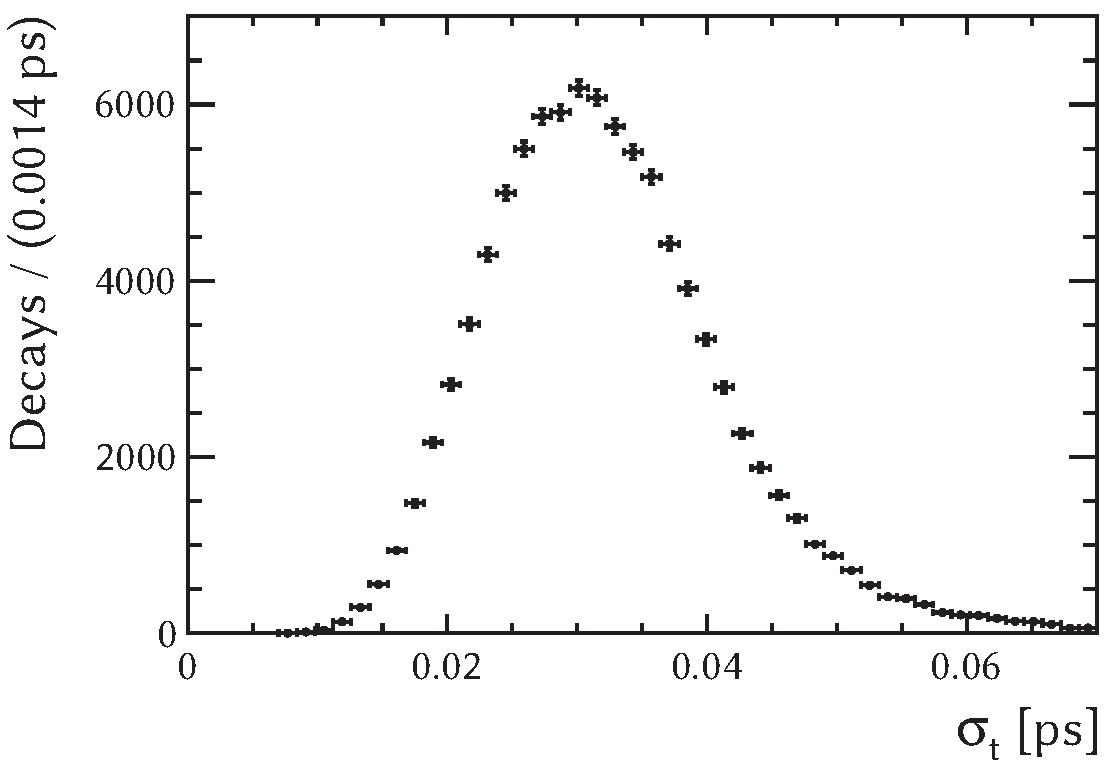
\includegraphics[width=0.5\textwidth]{graphics/analysis/sigmat}
  \caption{Distribution of \BstoJpsiKK{} signal decays in the estimated decay-time uncertainty.}
  \label{fig:sigmat}
\end{figure}

Decay-time resolution is included in the model for the signal decay by convolving the theoretical model with the model for the difference
between the measured time and the true time. This convolution is the integral of the two-dimensional PDF of the true and measured decay
times over all possible values of the former:
\begin{equation}
  P_\text{meas}(t_\text{meas}, \Omega)
    \equiv \int_0^\infty \ud t_\text{true}\, R(t_\text{meas} - t_\text{true}|\sigmat)\, P_\text{true}(t_\text{true}, \Omega)\ ,
\end{equation}
where $R$ is the PDF for the difference between the measured and true times, or the \emph{resolution model}. The resolution model is
conditional on $\sigmat$., i.e. normalized with respect to decay time for each individual value of $\sigmat$.

Although the resolution model is approximated by a Gaussian PDF with width $\sigmat$, a more sophisticated model is required to describe
the resolution in the PDF with sufficient precision. The model is a sum of two Gaussian PDFs with a common, non-zero mean and a width that
depends quadratically on $\sigmat$. The width of the first Gaussian PDF is approximately equal to $\sigmat$, while the width of the second
Gaussian PDF is roughly a factor two larger.

The double-Gaussian model is based on and validated with both simulated \BstoJpsiKK{} decays and prompt background decay candidates. Since
all tracks of prompt background candidates originate from the primary vertex, their ``true'' decay time is equal to zero and the
distribution of measured decay times is essentially the resolution model. Studies of the model and its parameters are described in detail
in references~\cite{Aaij:2015} and \cite{LHCb-ANA-2014-039}. The values of the resolution parameters are fixed in the fit of decay time and
angles. Uncertainties in the parameter values are propagated after the fit and accounted for as systematic uncertainties (see
Section~\ref{sec:result_syst}).


%%%%%%%%%%%%%%%%%%%%%%%%%%%
\subsection{Acceptance}
\label{subsec:ana_time_acc}
%%%%%%%%%%%%%%%%%%%%%%%%%%%

To account for the efficiencies of the decay-candidate reconstruction and selection processes, the PDF is multiplied by an acceptance
function and re-normalized to create a new PDF. The acceptance is is modelled as a product of two functions of decay time and one function
of decay angles. The angular part will be discussed in Section~\ref{sec:ana_angles}. This section describes the two decay-time functions.

\subsubsection{Track-Reconstruction Acceptance}
The first part of the non-trivial acceptance in decay time originates from an inefficiency in the reconstruction of particle tracks. This
efficiency decreases for increasing distance between the track and the proton beams. Since the distance between the primary and secondary
vertex and, therefore, the decay time are correlated with the distance between the four \BstoJpsiKK{} tracks and the beams, the efficiency
also decreases with increasing decay time.

In the measurement presented here the track-reconstruction acceptance is modelled by an exponential function in \emph{true} decay time. The
advantage of this model is that its implementation in the model of the decay-time distribution is straightforward. An exponential function
can be absorbed in the $\eGst$ factor of the differential decay rate (Equation~\ref{eq:angCoefs}):
\begin{equation}
  \eGst \longrightarrow e^{\beta\,t}\,\eGst = e^{-(\Gs-\beta)\,t} \equiv e^{-\Gs^\text{eff}\,t}\ ,
\end{equation}
where $\beta$ is the parameter that quantifies the rate at which the efficiency changes as a function of decay time. The parameter
$\Gs^\text{eff}$\textequiv$\Gs$\textminus$\beta$ can now be included in the model in the place of the parameter $\Gs$.

The parameter $\beta$ has been determined by a combination of studies with real and simulated data~\cite{LHCb-ANA-2014-039}. Because of
changes in the online reconstruction algorithms between the 2011 and 2012 runs and the different proton-collision energies in these
periods, the corresponding values of $\beta$ are evaluated separately: $\beta_\text{2011}$\texteq\mbox{\tm0.0090\textpm0.0022\unitsp\invps}
and $\beta_\text{2012}$\texteq\mbox{\tm0.0124\textpm0.0019\unitsp\invps}. These values have to be compared with
$\Gs$\textapprox0.66\unitsp\invps.

Although there is no sensitivity in the \BstoJpsiKK{} data to the parameters $\Gs$, $\beta_\text{2011}$, and $\beta_\text{2012}$
separately, the value of $\Gs^\text{eff}$ can be determined in the fit of decay time separately for the 2011 and 2012 periods.
Reparameterizing, there is sensitivity for the combinations $\Gs$\textminus$\tfrac{1}{2}(\beta_\text{2011}$\textplus$\beta_\text{2012})$
and $\beta_\text{2012}$\textminus$\beta_\text{2011}$.

To combine the information on the difference between the two $\beta$ values with the externally determined values, the $\beta$ parameters
are varied with constraints in the time and angular fit. These constraints are implemented by adding a parabolic term to the NLL of the
form $\frac{1}{2\hat{\sigma}^2}(\beta-\hat{\beta})^2$ for each parameter, where the external value is denoted by $\hat{\beta}$ and the
external uncertainty by $\hat{\sigma}$. Because these external constraints are much tighter than the constraints from the \BstoJpsiKK{}
data, the values that are estimated in the fit are comparable to the external values:
$\beta_\text{2011}$\texteq\mbox{\tm0.0086\textpm0.0021\unitsp\invps} and
$\beta_\text{2012}$\texteq\mbox{\tm0.0127\textpm0.0018\unitsp\invps}.

There are some limitations to this model of the track-reconstruction acceptance. The model is implemented for true decay time, whereas the
external values of the $\beta$ parameters were evaluated with the measured decay time. In this measurement, this is assumed to be a good
approximation, because the time scale of the variations in the model is much larger than the resolution. That is,
$\beta^{-1}$\textapprox\mbox{\tenpow{2}\unitsp{}ps}\textgg\mbox{0.05\unitsp{}ps}.

Also the model itself is an approximation. As was shown in reference~\cite{LHCb-ANA-2014-039}, the shape of the acceptance is better
described by the function 1\textplus$\beta\,t$\textplus$\beta'\,t^2$ than by $e^{\beta\,t}$\textapprox1\textplus$\beta\,t$. A systematic
uncertainty in the parameter estimates corresponding to the assumption of the shape $e^{\beta\,t}$ is estimated in
Section~\ref{sec:result_syst}.

\subsubsection{Trigger Acceptance}
As described in Section~\ref{subsec:ana_bkgSub_sel}, there are also trigger requirements that introduce non-trivial acceptance effects in
decay time. The shapes of the acceptance functions corresponding to the decay-time biasing trigger categories are determined relative to
the shapes of the unbiased categories, which have a uniform acceptance function.

The shape of the trigger acceptance is described in bins of decay time. For each bin, numbers of decays are counted in the different
trigger categories to determine the relative efficiency in the bin. To also include information on the exponential shape of the decay in
the resulting binned acceptance function, the decay counts are varied in the fit of decay time and angles.

Since originally only the shape of the differential decay rate in time and angles is determined in the fit, additional terms need to be
included in the NLL to count decays in the different trigger categories. For unweighted decays the PDF for the number of decays in a
category would be a Poisson distribution, which is proportional to $\nu^n\,e^{-\nu}$, where $n$ is the observed number of decays and $\nu$
is the parameter for the expected number of decays. This PDF would give an additional NLL term of $\nu$\textminus$n\,\ln\nu$. However,
because each decay candidate is counted with its signal weight, this term is modified to obtain the correct uncertainty on the parameter
$\nu$ from a maximum-likelihood fit.

Instead of only replacing the variable $n$ in the Poissonian NLL term by the sum of the decay-candidate weights, the term is also
multiplied by weight factor:
\begin{equation}
  \frac{\sum w}{\sum w^2}\left( \nu - \ln\nu\,\sum w \right)\ ,
\end{equation}
where $\sum w$ is the sum of the decay weights and $\sum w^2$ the sum of the squared decay weights. This function reaches its minimum at
$\nu$\texteq$\sum w$, so the estimated value for $\nu$ in a maximum-likelihood fit with only this function would be the sum of the decay
weights. The inverse of the second derivative of the function, from which the uncertainty in $\nu$ is estimated, is given by $\sum w^2$
instead of $\sum w$ for an unmodified Poisson term. The former number is equal to the variance that is expected when counting weighted
decay candidates.

\begin{itemize}
  \item describe trigger categories and efficiency parameters
  \item using all categories (6) vs merging categories (4 or 5)
  \item short description of resulting acceptance functions (plots): $\longrightarrow$ Roel
\end{itemize}

%Since only decay candidates that are selected by the HLT2-biased trigger line are used for the fit of decay time and angles, only the
%trigger-acceptance functions for the HLT1-unbiased/HLT2-biased and exclusively-HLT1-biased/HLT2-biased combinations are required.

\begin{figure}[htbp]
  \centering
  \begin{subfigure}{0.49\textwidth}
    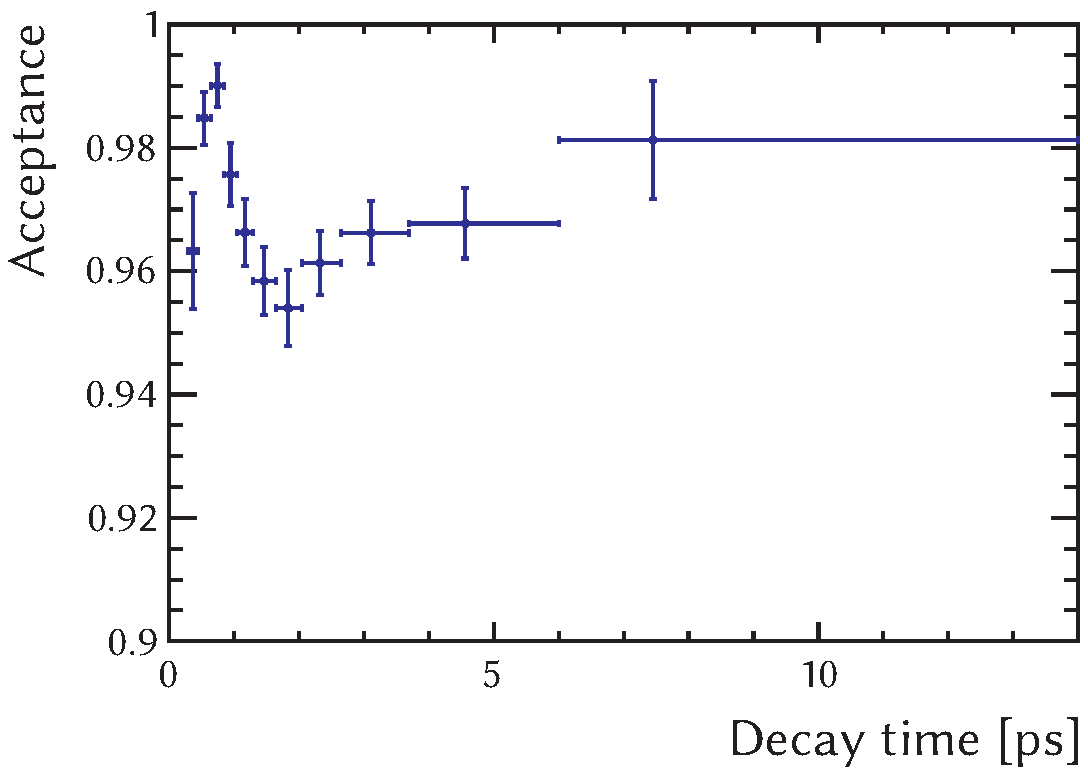
\includegraphics[width=\textwidth]{graphics/analysis/trigTimeAcc_2011_UB}
    \caption{}
    \label{fig:trigAcc_2011_UB}
  \end{subfigure}%
  \hfill%
  \begin{subfigure}{0.49\textwidth}
    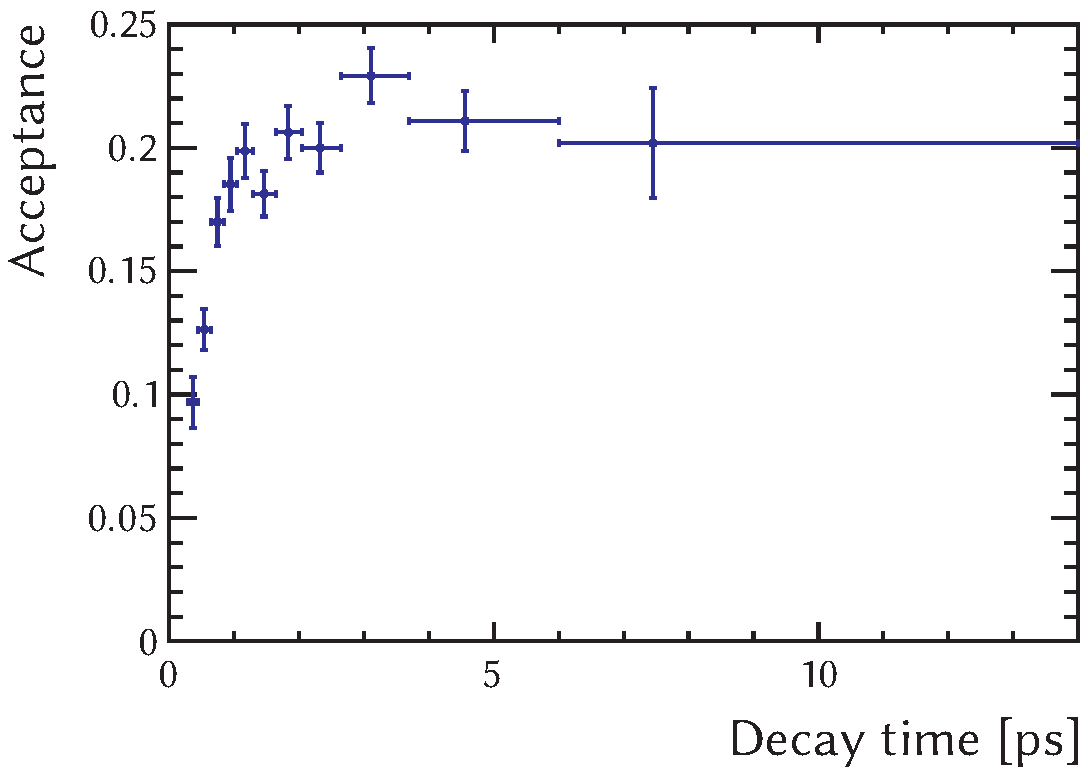
\includegraphics[width=\textwidth]{graphics/analysis/trigTimeAcc_2011_exclB}
    \caption{}
    \label{fig:trigAcc_2011_exclB}
  \end{subfigure}

  \vspace*{0.02\textwidth}
  \begin{subfigure}{0.49\textwidth}
    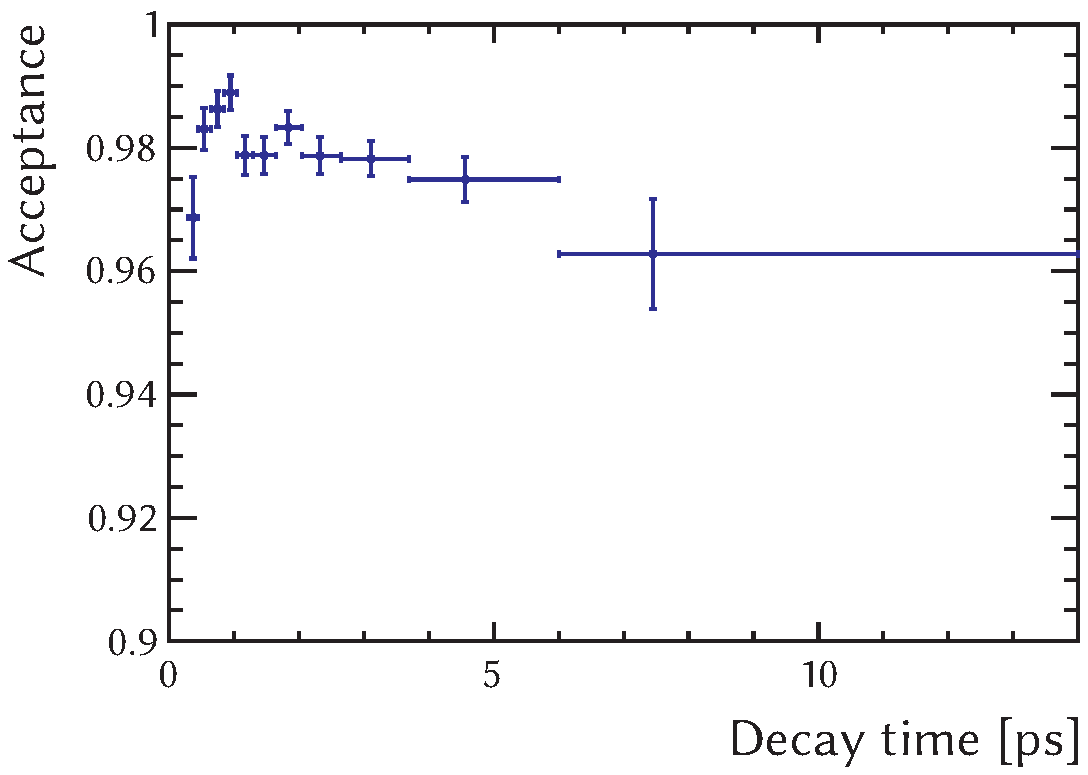
\includegraphics[width=\textwidth]{graphics/analysis/trigTimeAcc_2012_UB}
    \caption{}
    \label{fig:trigAcc_2012_UB}
  \end{subfigure}%
  \hfill%
  \begin{subfigure}{0.49\textwidth}
    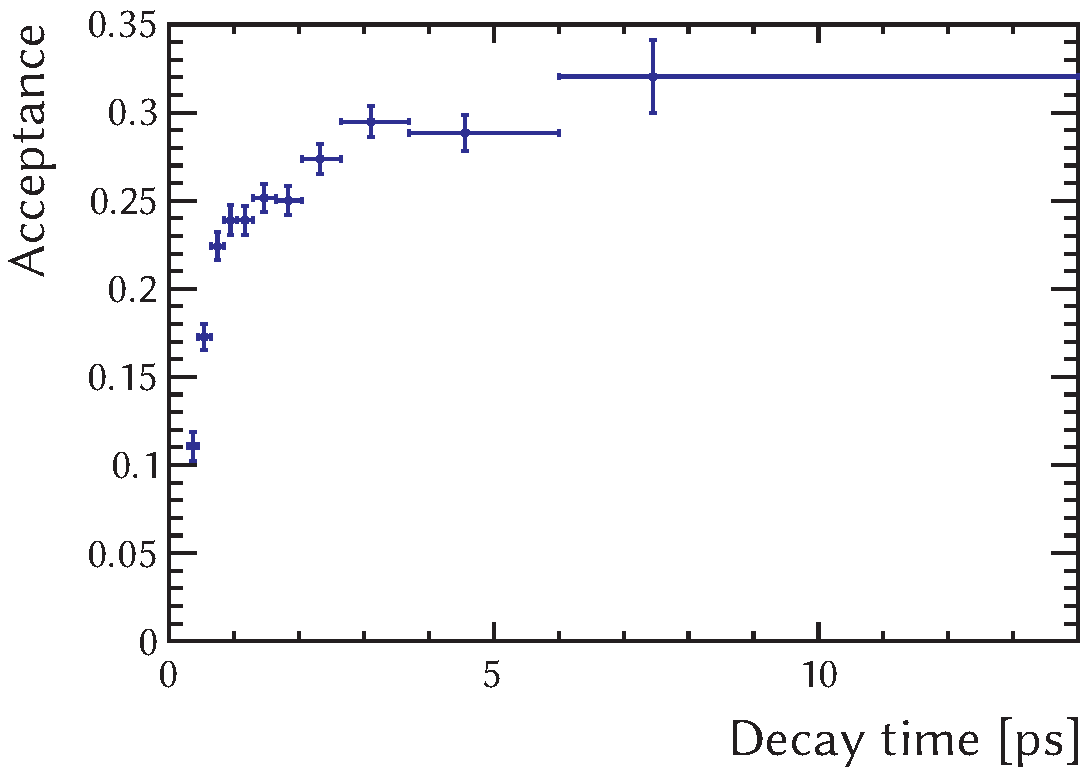
\includegraphics[width=\textwidth]{graphics/analysis/trigTimeAcc_2012_exclB}
    \caption{}
    \label{fig:trigAcc_2012_exclB}
  \end{subfigure}
  \caption{Trigger acceptance in bins of decay time for (a, b) the 2011 run and (c, d) the 2012 run
           and for (a, c) the HLT1-unbiased/HLT2-biased selection and (b, d) the exclusively-HLT1-biased/HLT2-biased selection.
           Notice that the efficiency range of the HLT1-unbiased/HLT2-biased graphs is 90--100\%.
           Because the absolute efficiency of the HLT1 selections is unknown, the scales of the efficiencies
           in the graphs are given with respect to the efficiency of the HLT1-unbiased selection.}
  \label{fig:trigAcc}
\end{figure}


\section{Decay Angles}
\label{sec:ana_angles}

Also the measurement of the decay angles has a finite precision and is affected by a non-trivial acceptance shape. Whereas resolution
effects in decay time directly affect the amplitude of the measured decay-time oscillation and, therefore, the estimates of the
CP-violation parameters, the effect of angular resolution are indirect and expected to be smaller. Because a convolution of the angular
functions in the decay model with a resolution function would be far from trivial, angular resolution is not included in the model of the
decay. However, resolution effects cannot be neglected and introduce systematic uncertainties in the final parameter estimates (see
Section~\ref{sec:result_syst}).

The acceptance as a function of decay angles is included in the decay model. Its shape is shown in Figure~\ref{fig:angAcc}. The figure
shows the acceptance function for each of three angles, integrated over the two remaining angles. The data points are sums of simulated
decays, weighted by the inverse of the PDF that was used to generate the decays at each point in decay angles. This results in the ratio of
the observed distribution including acceptance effects and the generated distribution. The shape of this ratio in the decay angles is given
by the shape of the angular acceptance function. In essence this is also how the acceptance function for the decay model, represented by
the blue line, is determined.

\begin{figure}[tbp]
  \centering
  \begin{subfigure}{0.49\textwidth}
    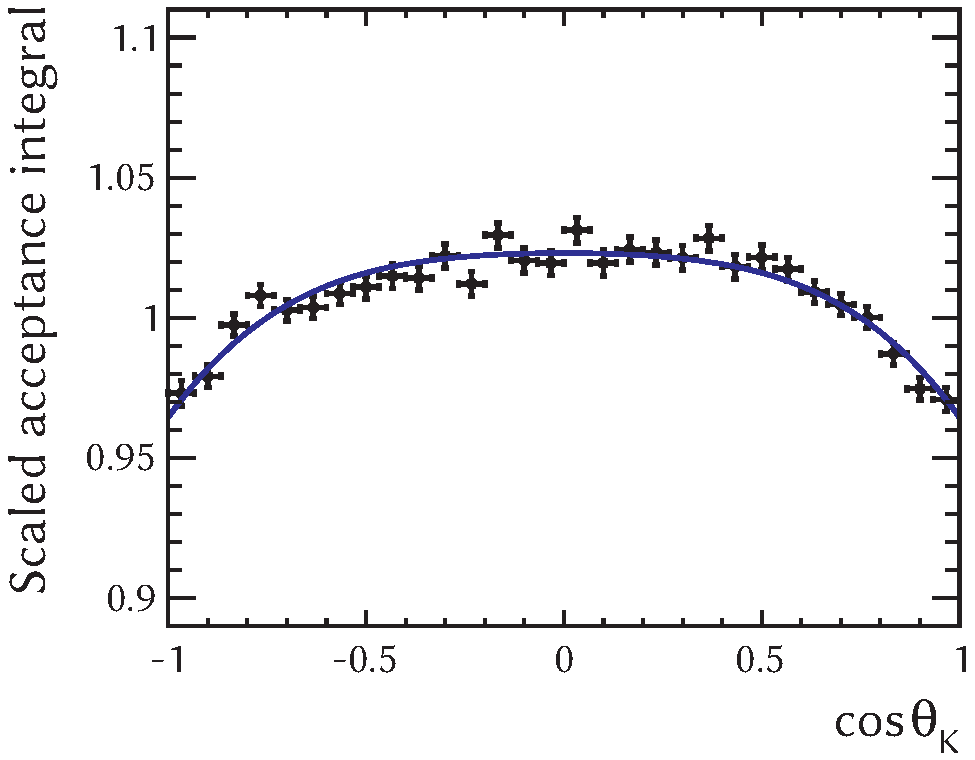
\includegraphics[width=\textwidth]{graphics/analysis/angAcc_ctk}
    \caption{}
    \label{fig:angAcc_ctk}
  \end{subfigure}%
  \hfill%
  \begin{subfigure}{0.49\textwidth}
    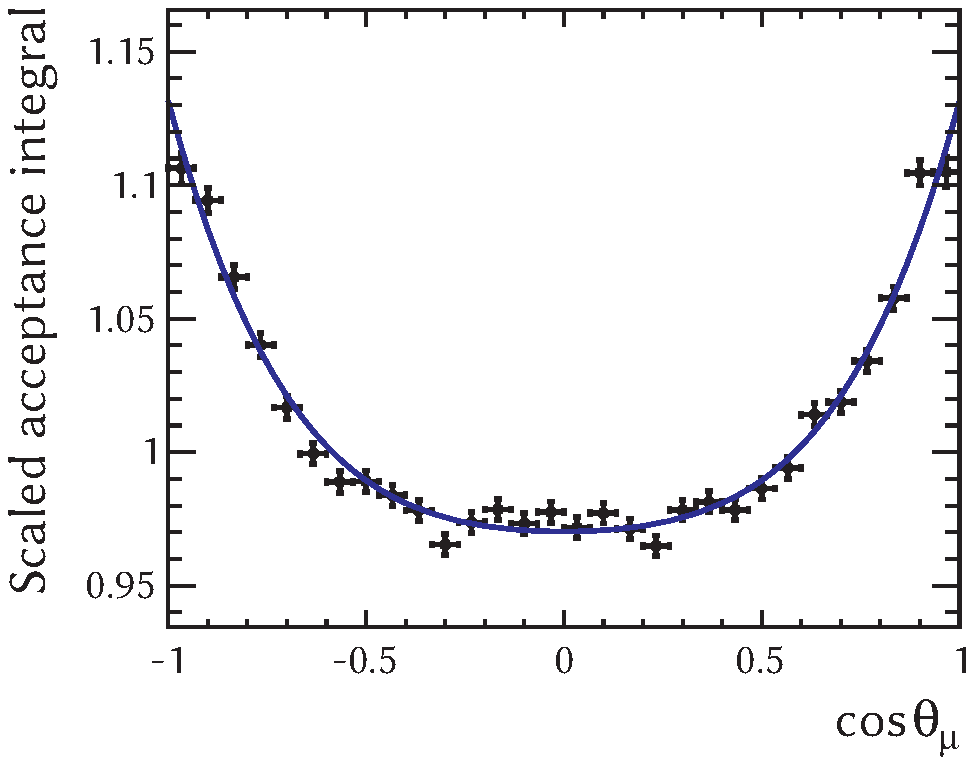
\includegraphics[width=\textwidth]{graphics/analysis/angAcc_ctl}
    \caption{}
    \label{fig:angAcc_ctl}
  \end{subfigure}

  \vspace*{0.02\textwidth}
  \begin{subfigure}{0.49\textwidth}
    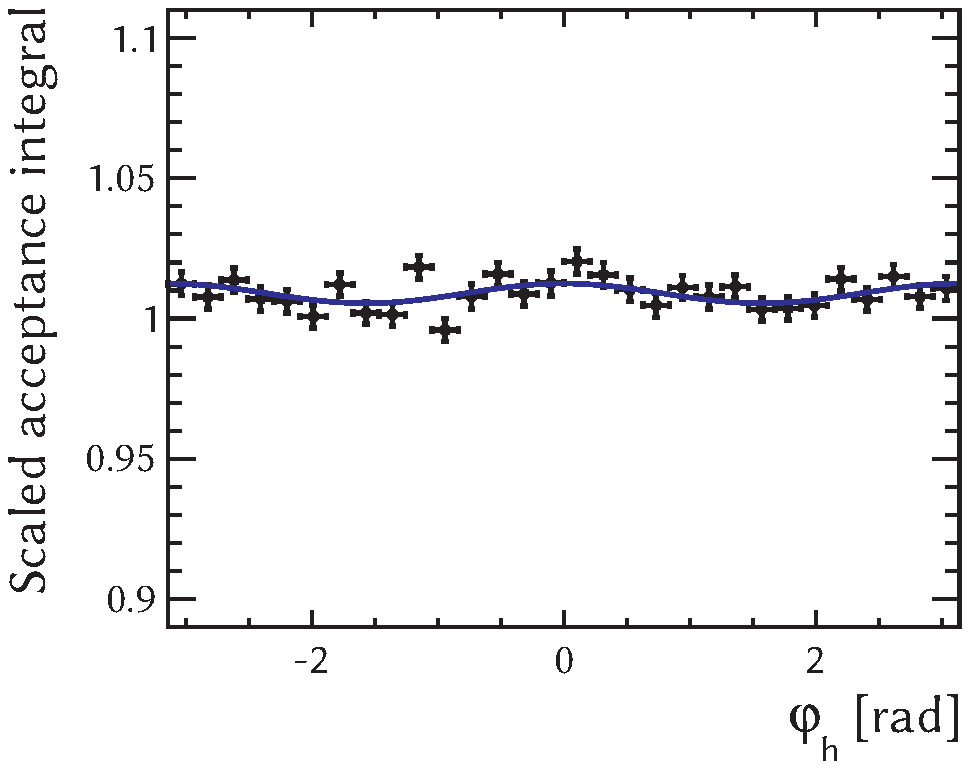
\includegraphics[width=\textwidth]{graphics/analysis/angAcc_phi}
    \caption{}
    \label{fig:angAcc_phi}
  \end{subfigure}
  \caption{Shape of the acceptance function in each of the three decay angles: (a) $\cthetaK$, (b) $\cthetal$, (c) $\phihel$.
           The angular acceptance function is integrated over the two remaining angles in each of the figures.
           The blue line represents a parameterization of the function in terms of Legendre polynomials for $\cthetaK$
           and real-valued spherical harmonics for $\cthetal$ and $\phihel$.
           The data points are obtained by a sum over simulated decays, which are weighted by the value of the PDF that was used to
           generate the decays at each point in decay angles.
           Notice that the vertical scale of these figures does not start at zero.}
  \label{fig:angAcc}
\end{figure}

The ratio of observed and generated angular PDFs can be written as
\begin{equation}
  \begin{aligned}
    \frac{P^\text{obs}(\Omega|t)}{P^\text{gen}(\Omega|t)}
        &= \frac{\effta\, p(t,\Omega)}{\int\ud\Omega\; \effta\, p(t,\Omega)}\; \frac{\int\ud\Omega\; p(t,\Omega)}{p(t,\Omega)}\\
         = &\frac{\effta\, \int\ud\Omega\; p(t,\Omega)}{\int\ud\Omega\; \effta\, p(t,\Omega)}
         = \frac{\effta}{\int\ud\Omega\; \effta\, P^\text{gen}(\Omega|t)}
         = \frac{\effta}{\meff(t)}\\
        \effta &= \meff(t)\; \frac{P^\text{obs}(\Omega|t)}{P^\text{gen}(\Omega|t)} \ ,
  \end{aligned}
  \label{eq:angAccPDFRatio}
\end{equation}
where $P^\text{obs}$ is the observed PDF, $P^\text{gen}$ the generated PDF, $p$ the function of time and angles from which the PDFs are
built, and $\eff$ the time and angular acceptance function. Both angular PDFs are conditional on decay time. The angular mean of the
acceptance function, which depends on decay time, is given by
\begin{equation}
  \meff(t) \equiv \int\ud\Omega\, \effta\, P^\text{gen}(\Omega|t)\ .
\end{equation}

Assuming the time and angular acceptance functions factorize, that is $\effta = \efft \times \effa$, the mean acceptance can be expressed
as
\begin{equation}
  \meff(t) = \efft \times \int\ud\Omega\, \effa\, P^\text{gen}(\Omega|t)
           = \efft \times \meffa(t) \ .
\end{equation}
Inserting this expression into the last line of Equation~\ref{eq:angAccPDFRatio} yields for the acceptance function
\begin{equation}
  \effta = \efft \times \meffa(t)\; \frac{P^\text{obs}(\Omega|t)}{P^\text{gen}(\Omega|t)}\ ,
\end{equation}
which means that the angular acceptance function is given by
\begin{equation}
  \label{eq:angAcc}
  \effa = \meffa(t)\; \frac{P^\text{obs}(\Omega|t)}{P^\text{gen}(\Omega|t)}\ .
\end{equation}
The factor $\meffa(t)$ is the mean of the angular acceptance function, which generally depends on decay time. Since only the shape of the
angular acceptance function is relevant in this model, it is not required to determine the value of this angular constant factor. The ratio
of the observed and generated PDFs suffices to determine the shape of the function in the decay angles.


%%%%%%%%%%%%%%%%%%%%%%%%%%%%%%%%%%%%%%%%
\subsection{Acceptance Parameterization}
\label{subsec:ana_angles_param}
%%%%%%%%%%%%%%%%%%%%%%%%%%%%%%%%%%%%%%%%

The function $\effa$ is represented in Figure~\ref{fig:angAcc} by the blue line. For this figure, it is parameterized in terms of Legendre
polynomials and real-valued spherical harmonics, $\Lp{i}(\cthetaK)\,\rsph{l}{m}(\cthetal,\phihel)$ (see also
Section~\ref{sec:angularDecay_squareAmp}, Equations~\ref{eq:PYdef} and \ref{eq:realYdef}). These functions form an orthogonal basis of
functions of the three decay angles.

In principle an arbitrary function is expressed as an infinite sum of basis functions, but in practice the relatively uniform acceptance
function can be described by a limited number of contributions. The function $\Lp{0}\,\rsph{0}{0}$ is a constant and would be the only
contribution for a truly uniform acceptance function. A few higher-order functions up to $i$\texteq4, $l$\texteq4, and $m$\texteq2 are
included to describe the shape shown in Figure~\ref{fig:angAcc}. Even higher orders represent faster changes in the acceptance function and
can be omitted for this slowly-changing shape.

The coefficients of the basis functions, which specify the shape of the acceptance function, are determined from the simulated
\BstoJpsiKK{} decays that were used for Figure~\ref{fig:angAcc}. Expressing the acceptance function as
\begin{equation}
  \effa = \sum_{i,l,m} c_{ilm}\,b_{ilm}(\Omega)\ ,
\end{equation}
the coefficients are defined as
\begin{equation}
  \label{eq:angEffCoefDef}
  c_{ilm} \equiv (i+\tfrac{1}{2}) \int\ud\Omega\,b_{ilm}(\Omega)\,\effa\ ,
\end{equation}
where $b_{ilm}$ is a basis function and $c_{ilm}$ the corresponding coefficient. The normalization factor $i+\tfrac{1}{2}$ arises from
the fact that Legendre polynomials are orthogonal, but not orthonormal:
\begin{equation}
  \int\ud\cthetaK\,\Lp{i}(\cthetaK)\cdot\Lp{i}(\cthetaK) = \frac{1}{i+\tfrac{1}{2}}\ .
\end{equation}

The integral in Equation~\ref{eq:angEffCoefDef} is calculated by means of Monte Carlo integration, using the simulated decays. A constant
is defined to absorb the factor $\meffa(t)$ in Equation~\ref{eq:angAcc}:
\begin{equation}
  \label{eq:angEffConst}
  E_a \equiv \left[ \int\ud t\, \frac{P^\text{obs}(t)}{\meffa(t)} \right]^{-1}\ .
\end{equation}
Notice that $E_a$ reduces to the mean angular acceptance, $\meffa$, if the PDFs for time and angles factorize,
$P^\text{gen}(t,\Omega)$\texteq$P^\text{gen}(t)$\texttimes$P^\text{gen}(\Omega)$. In this case $P^\text{gen}(\Omega|t)$ is equal to
$P^\text{gen}(\Omega)$ and $\meffa$ is independent of time and the integral in Equation~\ref{eq:angEffConst} evaluates to $\meffa^{-1}$.

With the constant $E_a$ and the definition of the angular acceptance in Equation~\ref{eq:angAcc}, the coefficients of
Equation~\ref{eq:angEffCoefDef} can be expressed as
\begin{equation}
  \label{eq:angAccInt}
  \begin{split}
    \tfrac{1}{E_a}\, c_{ilm} &= \int\ud t\, \frac{P^\text{obs}(t)}{\meffa(t)}
                                \cdot (i+\tfrac{1}{2}) \int\ud\Omega\,b_{ilm}(\Omega)\, \effa \\
                             &= (i+\tfrac{1}{2}) \int\ud t\, \ud\Omega\; \frac{P^\text{obs}(t)}{\meffa(t)}\,
                                b_{ilm}(\Omega)\, \meffa(t)\, \frac{P^\text{obs}(\Omega|t)}{P^\text{gen}(\Omega|t)} \\
                             &= (i+\tfrac{1}{2}) \int\ud t\, \ud\Omega\; P^\text{obs}(t,\Omega)\,
                                \frac{b_{ilm}(\Omega)}{P^\text{gen}(\Omega|t)} \ .
  \end{split}
\end{equation}
The value of this integral is estimated with a sum over simulated decays:
\begin{equation}
  E\left( \tfrac{1}{E_a}\, c_{ilm} \right)
      = (i + \tfrac{1}{2})\, \frac{1}{N^\text{obs}}\, \sum_{e=1}^{N^\text{obs}}\frac{b_{ilm}(\Omega_e)}{P^\text{gen}(\Omega_e|t_e)}
  \label{eq:angEffCoefEst}
\end{equation}
Since the ``mean acceptance'' is a constant equal for all coefficients, this factor can be ignored for the shape of the acceptance
function. The values of the coefficients that were used for the function in Figure~\ref{fig:angAcc} are specified in
Table~\ref{tab:angEffCoefs}.
\begin{table}[htbp]
  \centering
  \caption{Values of the coefficients of the angular acceptance function that were used for the function shown in Figure~\ref{fig:angAcc}.
           The specified values are estimates of the quantity $\tfrac{1}{E_a}\, c_{ilm}$ (Equation~\ref{eq:angEffCoefEst}).}
  \label{tab:angEffCoefs}
  \begin{tabular}{ccc}
    \hline
    coefficient ($ilm$)  &  value  &  statistical uncertainty  \\
    \hline
    000  &   3.5767  &  0.0011  \\
    020  &  +0.1535  &  0.0030  \\
    040  &  +0.0305  &  0.0031  \\
    022  &  +0.0096  &  0.0026  \\
    200  &  -0.125   &  0.006   \\
    400  &  -0.033   &  0.008   \\
    \hline
  \end{tabular}
\end{table}

For a uniform acceptance function, $\effa$\texteq$\meffa$\texteq constant, and Equation~\ref{eq:angAccInt} reduces to
\begin{equation}
  \tfrac{1}{E_a}\, c_{ilm} = (i+\tfrac{1}{2}) \int\ud\Omega\,b_{ilm}(\Omega)\ .
\end{equation}
This integral is only non-zero for $i$\texteq$l$\texteq$m$\texteq0, for which $\tfrac{1}{E_a}\,c_{000}$\texteq2$\sqrt{\pi}$\textapprox3.54.
Table~\ref{tab:angEffCoefs} shows that the acceptance function is not too far from being uniform.


%%%%%%%%%%%%%%%%%%%%%%%%%%%%%%%%%
\subsection{Acceptance Normalization Weights}
\label{subsec:ana_angles_weights}
%%%%%%%%%%%%%%%%%%%%%%%%%%%%%%%%%

In principle the parameterization of the acceptance function in terms of Legendre polynomials and spherical harmonics could be used to
describe the acceptance function in the PDF for the time and angular fit. However, this would require criteria that specify which set of
basis functions to include in the description and a study of the effect of not including functions that are not in this set. A slightly
different approach circumvents this problem and includes all relevant acceptance information.

Using the notation of Equation~\ref{eq:angAccPDFRatio}, the PDF including acceptance effects is given by
\begin{equation}
  \label{eq:obsPDF}
  P^\text{obs}(t,\Omega) = \frac{\effta\, p(t,\Omega)}{\int\ud t\, \ud\Omega\; \effta\, p(t,\Omega)}
\end{equation}
Assuming the time and angular acceptance functions factorize and writing the function $p(t,\Omega)$ in the normalization integral as a sum
of angular terms (see Sections~\ref{sec:pheno_angles} and \ref{sec:pheno_equations}), the PDF can be expressed as
\begin{equation}
  \label{eq:obsPDFNormSum}
  P^\text{obs}(t,\Omega) = \efft\,\effa\, \frac{p(t,\Omega)}{\sum_k \int\ud t\, \efft f_t(t) \int\ud\Omega\, \effa f_{a,k}(\Omega)}
\end{equation}

If the angular acceptance function does not contain any free parameters, the factor $\effa$ in Equation~\ref{eq:obsPDFNormSum} becomes a
constant term in the minimization of the NLL (see also Section~\ref{sec:ana_fit}) and can be ignored. The angular acceptance function then
only remains in the normalization integral $\int\ud\Omega\, \effa f_{a,k}(\Omega)$. This integral is very similar to the integral in
Equation~\ref{eq:angEffCoefDef} and can be estimated in the same way (Equations~\ref{eq:angAccInt} and \ref{eq:angEffCoefEst}).

This procedure leads to the definition of \emph{normalization weights}, which were first described in \cite{duPree:2010}. The weights are
determined for each term in the differential decay rate and are defined by
\begin{equation}
  \label{eq:angNormWeightDef}
  \xi_k \equiv \int\ud\Omega\, \effa f_{a,k}(\Omega)\ ,
\end{equation}
with a corresponding estimate from simulated events
\begin{equation}
  \label{eq:angNormWeightEst}
  E\left( \tfrac{1}{E_a}\, \xi_k \right)
      = \frac{1}{N^\text{obs}}\, \sum_{e=1}^{N^\text{obs}}\frac{f_{a,k}(\Omega_e)}{P^\text{gen}(\Omega_e|t_e)}\ .
\end{equation}
The estimated values of the normalization weights are given in Table~\ref{tab:angNormWeights}.
\begin{table}[htbp]
  \centering
  \caption{Values of the normalization weights of the angular acceptance function.
           The specified values are estimates of the quantity $\tfrac{1}{E_a}\, \xi_k$ (Equation~\ref{eq:angNormWeightEst}).}
  \label{tab:angNormWeights}
  \begin{tabular}{ccc}
    \hline
    weight ($k$)  &  value  &  statistical uncertainty  \\
    \hline
    00                    &  0.9744   &  0.0005  \\
    $\parallel\parallel$  &  1.0245   &  0.0006  \\
    $\perp\perp$          &  1.0263   &  0.0006  \\
    0$\parallel$          &  +0.0001  &  0.0005  \\
    0$\perp$              &  -0.0003  &  0.0004  \\
    $\parallel\perp$      &  -0.0006  &  0.0007  \\
    SS                    &  0.9896   &  0.0004  \\
    0S                    &  +0.0007  &  0.0014  \\
    $\parallel$S          &  +0.0007  &  0.0006  \\
    $\perp$S              &  +0.0003  &  0.0006  \\
    \hline
  \end{tabular}
\end{table}

\emph{to do:}
\begin{itemize}
  \item \emph{check signs in table}
  \item \emph{describe conversion between weights and basis coefficients}
\end{itemize}

\section{\texorpdfstring{$\KK$}{KK}-Mass Integrals}
\label{sec:ana_KKIntegrals}

As discussed in Sections~\ref{sec:pheno_KKMass} and \ref{subsec:pheno_equations_symmetry}, the dependence of the differential decay rate on
$\KK$ mass is summarized in the PDF by the quantities $\CSP$ and $\thetaSP$, which represent the $\KK$-mass integral of the rate. A
separate PDF is constructed for each interval in $\KK$ mass, with values of $\CSP$ and $\thetaSP$ that correspond to the $\KK$-mass shapes
in the interval.

The phase $\thetaSP$ is absorbed in the phase difference between the $\Jpsiphi$ and the S-wave amplitudes (see
Equations~\ref{eq:couplingFacAmps} and \ref{eq:phaseDiffDef}), which is measured for each interval. In principle, the $\CSP$ values could
also be measured, but because these factors only modify the magnitudes of the small S-wave interference terms more data would be needed for
a sensible measurement. For this measurement the $\CSP$ factors are computed and fixed in the fit of time and angles.

The decay model of Chapter~\ref{chap:pheno} is integrated over $\KK$ mass, where it is assumed the mass shape of the \BstoJpsiphi{} decay
is described by a relativistic Breit-Wigner function (see e.g.\ reference \cite{PDG}) and the $\KK$ S-wave contribution to the
\BstoJpsiKK{} decay by a Flatt\'e function~\cite{Flatte:1976xu}. Because the $\KK$-mass measurement has a finite resolution of
approximately 1\unitsp{}\MeV, these functions are convoluted with a resolution function, which is determined from the resolution in
simulated decays (see Reference~\cite{LHCb-ANA-2014-039}). The resulting $\CSP$ factors are listed in the third column of
Table~\ref{tab:CSPFactors}.
% $\fzero$ Flatt\'e parameters from \cite{Ablikim:2004wn}, resolution from MC

\begin{table}[htb]
  \centering
  \caption{S-wave--$\Jpsiphi$ coupling factors in the six $\KK$-mass intervals ($\CSP^i$).
           The $\CSP$ factors are computed for three different scenarios~\cite{LHCb-ANA-2014-039}:
           the nominal $\KK$-mass model with a Flatt\'e mass shape for the S-wave and the mass resolution estimated with simulated decays,
           a scenario with a 20\% worse $\KK$-mass resolution, and a scenario with a uniform $\KK$-mass shape for the S-wave.}
  \label{tab:CSPFactors}
  \begin{tabular}{ccccc}
    int.    &  KK mass [\MeV]   &  nominal  &  +20\% resolution  &  uniform S-wave  \\
    \hline
    1       &  \ \ 990 -- 1008  &  0.9178   &  0.9152            &  0.9586          \\
    2       &  1008 -- 1016     &  0.9022   &  0.8797            &  0.9110          \\
    3       &  1016 -- 1020     &  0.8619   &  0.8357            &  0.8618          \\
    4       &  1020 -- 1024     &  0.8875   &  0.8599            &  0.8828          \\
    5       &  1024 -- 1032     &  0.9360   &  0.9207            &  0.9227          \\
    6       &  1032 -- 1050     &  0.9641   &  0.9624            &  0.9110          \\
  \end{tabular}
\end{table}

Systematic uncertainties related to the assumed mass shapes and resolution are evaluated by varying these inputs (see
Section~\ref{sec:result_syst}). To this end the $\CSP$ factors are recalculated with a 20\% worse $\KK$-mass resolution (fourth column in
Table~\ref{tab:CSPFactors}) and with a uniform $\KK$-mass shape for the S-wave (fifth column in Table~\ref{tab:CSPFactors}).

\section{Flavour Tagging}
\label{sec:ana_tagging}

In Chapter~\ref{chap:pheno} the expressions for the differential decay rates of $\Bs$ and $\Bsbar$ decays are distinguished by the
variable $\qf$, which takes the value \tp1 for $\Bs$ and \tm1 for $\Bsbar$. Equation~\ref{eq:timeqfDep} in Section~\ref{sec:pheno_time}
shows the dependence on this variable.

As explained in Section~\ref{subsec:intro_LHCb_LHC}, it is experimentally not possible to determine whether the produced meson was $\Bs$
and $\Bsbar$ for each individual decay. Instead, this meson flavour is estimated for each decay, together with a probability that the
estimate is wrong. This \emph{flavour tag} is denoted by $\qt$, which takes the values \tp1 for a $\Bs$ estimate and \tm1 for a $\Bsbar$
estimate. The estimate of the wrong-tag probability is denoted by $\etaTag$.

For either value of $\qt$ the differential rate is a sum of the rates for true $\Bs$ ($\qf$\texteq\tp1) and true $\Bsbar$
($\qf$\texteq\tm1), where the relative contributions depend on the wrong-tag probability. For small wrong-tag probability the two
contributions are well separated, which enables the measurement of the oscillation amplitude from which the main sensitivity to
CP-violation parameters originates (see Section~\ref{sec:pheno_equations}). If the wrong-tag probability becomes larger, the opposite
oscillations of true $\Bs$ and true $\Bsbar$ start to cancel.

Decay candidates are assigned to different \emph{flavour-tagging categories} according to the estimate of the wrong-tag probability. For
the main measurement the candidates are only classified as \emph{tagged} (0\textlt$\etaTag$\textle0.5) or \emph{untagged}
($\etaTag$\texteq0.5). For tagged decay candidates the decay model depends on the value of $\etaTag$ for each candidate. For untagged
candidates the flavour-tagging algorithms are unable to estimate the $\Bs$ flavour. For these candidates the wrong-tag probability is 50\%
by definition.

Although the implementation of flavour tagging that uses the value of $\etaTag$ for each individual decay candidate is more optimal, the
analysis can be simplified by using an average wrong-tag probability for tagged candidates. In this case the tagging information can be
used more optimally by defining several categories of tagged events, such that candidates with small and large wrong-tag probabilities are
separated. This is achieved by defining ranges in $\etaTag$.

In summing the contributions of true $\Bs$ and true $\Bsbar$ any asymmetries in their production and detection should be taken into
account. The LHC collides protons, which contain more matter than antimatter. This creates a small matter--antimatter asymmetry in the
fragmentation and hadronization processes and consequently a small asymmetry in the numbers of $\Bs$ and $\Bsbar$ that are produced. In
addition, the flavour-tagging process relies on the detection of charged kaons, which is asymmetric for $\Kp$ and $\Km$. This creates a
difference in the fractions of the $\Bs$ and $\Bsbar$ decays in each tagging category.


%%%%%%%%%%%%%%%%%%%%%%%%%%%%%%%
\subsection{Formalism}
\label{subsec:ana_tagging_form}
%%%%%%%%%%%%%%%%%%%%%%%%%%%%%%%

The effect of any of $\Bs$--$\Bsbar$ normalization asymmetries on the differential decay rate can be written in the form 1\textplus$\qf\,
A$, where the asymmetry is denoted by $A$. Examining Equation~\ref{eq:timeqfDep}, an additional normalization asymmetry arises from CP
violation in mixing. The factor $1-\qf\,\Cm$ is included as an asymmetry contribution, with $A$\texteq\tm$\Cm$.

Exploiting the relation $\qf^2$\texteq\tp1, the product of all asymmetries can be expressed in a general form as
\begin{equation}
  \label{eq:asymProd}
  \prod_i (1+\qf\, A_i) \equiv \avgCEven + \qf\,\avgCOdd \ ,
\end{equation}
where $\avgCEven$ and $\avgCOdd$ are factors that contain the asymmetries, but not the variable $\qf$. Denoting the $\cDGs$ and $\sDGs$
terms as $\even$ (even under $\Bs\leftrightarrow\Bsbar$) and the $\cDms$ and $\sDms$ terms as $\odd$ (odd under
$\Bs\leftrightarrow\Bsbar$), the differential decay rate can be expressed as
\begin{equation}
  \label{eq:diffRateAsym}
  \begin{aligned}
    \frac{\ud^4\Gamma}{\ud t\, \ud\Omega}
      &= (\avgCEven + \qf\,\avgCOdd) (\even + \qf\,\odd) \\
      &= (\avgCEven + \qf\,\avgCOdd)\, \even + (\avgCOdd + \qf\,\avgCEven)\, \odd \ .
  \end{aligned}
\end{equation}

The two tagging algorithms that are used for the \BstoJpsiKK{} measurement give separate estimates of the $\Bs$ flavour and the
corresponding wrong-tag probability. The true wrong-tag probability for $\Bs$, which is a function of the estimated probability $\etaTag$,
is denoted by $\wTag$. Because of the $\Bs$--$\Bsbar$ asymmetries mentioned above, the probability for $\Bsbar$ decays has a different
dependence on $\etaTag$ and is denoted by $\wTagBar$.

Expressions for the differential rates of different combinations of opposite-side and same-side flavour tags can be derived by multiplying
the rates for true $\Bs$ and true $\Bsbar$ by the appropriate combinations of wrong-tag probabilities. Assuming the probabilities for the
opposite-side and same-side algorithms are uncorrelated and labelling the algorithms by ``o'' and ``s'', respectively, the resulting
rates are given by
\begin{alignat}{3}
  \label{eq:diffRateWTag}
  \qtOS=+1;\, \qtSS=-1:  &\quad&  (1-\wTagOS)(1-\wTagSS)           &\;& (\avgCEven+\avgCOdd)(\even+\odd) & \nonumber\\*
                         &     &  +\ \wTagBarOS\, \wTagBarSS       &  & (\avgCEven-\avgCOdd)(\even-\odd) & \nonumber\\
  \qtOS=+1;\, \qtSS=-1:  &     &  (1-\wTagOS)\, \wTagSS            &  & (\avgCEven+\avgCOdd)(\even+\odd) & \nonumber\\*
                         &     &  +\ \wTagBarOS\, (1-\wTagBarSS)   &  & (\avgCEven-\avgCOdd)(\even-\odd) & \nonumber\\
  \qtOS=-1;\, \qtSS=+1:  &     &  \wTagSS\, (1-\wTagOS)            &  & (\avgCEven+\avgCOdd)(\even+\odd) &          \\*
                         &     &  +\ (1-\wTagBarSS)\, \wTagBarOS   &  & (\avgCEven-\avgCOdd)(\even-\odd) & \nonumber\\
  \qtOS=-1;\, \qtSS=-1:  &     &  \wTagSS\, \wTagOS                &  & (\avgCEven+\avgCOdd)(\even+\odd) & \nonumber\\*
                         &     &  +\ (1-\wTagBarSS)(1-\wTagBarOS)  &  & (\avgCEven-\avgCOdd)(\even-\odd) & \nonumber\ .
\end{alignat}
Notice that the sum of the rates of the four cases is given by the expression in Equation~\ref{eq:diffRateAsym}, summing the rates of
$\qf$\texteq\tp1 and $\qf$\texteq\tm1.

Rewriting the expressions in Equation~\ref{eq:diffRateWTag}, the observed differential decay rate in one of the tagging categories can be
expressed in a form similar to Equation~\ref{eq:diffRateAsym}:
\begin{equation}
  \label{eq:diffRateTags}
  \left(\frac{\ud^4\Gamma}{\ud t\, \ud\Omega}\right)_{c,\,\qtOS,\,\qtSS}
      = \tagCatCoef[c]\, (\CEven\, \even + \COdd\, \odd) \ ,
\end{equation}
where the coefficients $\CEven$ and $\COdd$ both depend on the tagging category, $c$, and on the flavour tags, $\qtOS$ and $\qtSS$. The
parameter $\tagCatCoef[c]$ is the average of the fractions of true $\Bs$ and true $\Bsbar$ decays in the category. To express the
coefficients in terms of these quantities, a \emph{tagging-dilution factor} and a corresponding ``asymmetry'' are defined as
\begin{equation}
  \dil = 1 - \wTag - \wTagBar  \qquad\text{and}\qquad  \ADilWTag = \frac{\wTag-\wTagBar}{1 - \wTag - \wTagBar} \ .
\end{equation}
In general, all tagging parameters depend on the tagging category: $\dil[c]$, $\ADilWTag[c]$, $\avgCEven[c]$, and $\avgCOdd[c]$. In terms
of these parameters the coefficients $\CEven$ and $\COdd$ are given by
\begin{subequations}
  \label{eq:evenOddTagCoefs}
  \begin{align}
    2\,\CEven &\equiv \avgCEven[c]
                         + \qtOS\,\dilOS[c]\left(\avgCOdd[c] - \ADilWTagOS[c]\,\avgCEven[c] \right)
                         + \qtSS\,\dilSS[c]\left(\avgCOdd[c] - \ADilWTagSS[c]\,\avgCEven[c] \right) \nonumber\\
                         &\qquad\quad\
                           + \qtOS\,\qtSS\,\dilOS[c]\,\dilSS[c]\left[(1 + \ADilWTagOS[c]\,\ADilWTagSS[c])\,\avgCEven[c]
                                                                  - \ADilWTagOS[c]\,\ADilWTagSS[c]\,\avgCOdd[c] \right] \\
    2\,\COdd &\equiv \avgCOdd[c]
                        + \qtOS\,\dilOS[c]\left(\avgCEven[c] - \ADilWTagOS[c]\,\avgCOdd[c] \right)
                        + \qtSS\,\dilSS[c]\left(\avgCEven[c] - \ADilWTagSS[c]\,\avgCOdd[c] \right) \nonumber\\
                        &\qquad\quad\
                          + \qtOS\,\qtSS\,\dilOS[c]\,\dilSS[c]\left[(1 + \ADilWTagOS[c]\,\ADilWTagSS[c])\,\avgCOdd[c]
                                                                  - \ADilWTagOS[c]\,\ADilWTagSS[c]\,\avgCEven[c] \right] \ .
  \end{align}
\end{subequations}

Various limits can be considered for the $\CEven$ and $\COdd$ coefficients in Equations~\ref{eq:diffRateTags} and \ref{eq:evenOddTagCoefs}.
Without \BsBsbar{} normalization asymmetries the coefficients $\avgCEven$ and $\avgCOdd$ reduce to one and zero, respectively:
\begin{subequations}
  \begin{align}
    2\,\CEven &= 1
                 - \qtOS\,\dilOS[c]\,\ADilWTagOS[c]
                 - \qtSS\,\dilSS[c]\,\ADilWTagSS[c]
                 + \qtOS\,\qtSS\,\dilOS[c]\,\dilSS[c]\,(1 + \ADilWTagOS[c]\,\ADilWTagSS[c]) \\
    2\,\COdd &=  \qtOS\,\dilOS[c]
                 + \qtSS\,\dilSS[c]
                 - \qtOS\,\qtSS\,\dilOS[c]\,\dilSS[c]\,\ADilWTagOS[c]\,\ADilWTagSS[c] \ .
  \end{align}
\end{subequations}
Without any asymmetries, the coefficients are given by
\begin{subequations}
  \label{eq:evenOddTagCoefsNoAsym}
  \begin{align}
    2\,\CEven &= 1
                 + \qtOS\,\qtSS\,\dilOS[c]\,\dilSS[c] \\
    2\,\COdd &=  \qtOS\,\dilOS[c]
                 + \qtSS\,\dilSS[c] \ .
  \end{align}
\end{subequations}

In case only one of the two flavour tags is considered, the differential rate is given by the sum of the $\Bs$ and $\Bsbar$ rates of the
other tag. Considering only opposite-side tagging gives
\begin{subequations}
  \begin{align}
    \sum_{\qtSS} \CEven &= \avgCEven[c] + \qtOS\,\dilOS[c]\left(\avgCOdd[c]  - \ADilWTagOS[c]\,\avgCEven[c] \right) \\
    \sum_{\qtSS} \COdd  &= \avgCOdd[c]  + \qtOS\,\dilOS[c]\left(\avgCEven[c] - \ADilWTagOS[c]\,\avgCOdd[c]  \right) \ .
  \end{align}
\end{subequations}
Effectively this is the same as considering the candidates untagged for the same-side algorithm, which gives
$\wTag$\textequiv$\wTagBar$\textequiv0.5\textto$\dil$\texteq0. Without any flavour tags the coefficients are given by
\begin{subequations}
  \begin{align}
    \sum_{\qtOS,\qtSS} \CEven &= 2\,\avgCEven[c] \\
    \sum_{\qtOS,\qtSS} \COdd  &= 2\,\avgCOdd[c]  \ .
  \end{align}
\end{subequations}

Note that without flavour tagging, one is generally not interested in an expression of the differential decay rate that depends on the
tagging category. The sum of all rates cannot depend on flavour-tagging variables or parameters and should be given by
\begin{equation}
  \sum_{c,\,\qtOS,\,\qtSS} \left(\frac{\ud^4\Gamma}{\ud t\, \ud\Omega}\right)_{c,\qtOS,\qtSS}
    = 2\,\avgCEven[\text{S}]\, \even + 2\,\avgCOdd[\text{S}]\, \odd \ ,
\end{equation}
where the coefficients $\avgCEven[\text{S}]$ and $\avgCOdd[\text{S}]$ are defined as in Equation~\ref{eq:asymProd}, but including only
asymmetries that do not depend on tagging. As a result, the weighted sums of asymmetry coefficients over tagging categories are given by
\begin{equation}
  \label{eq:avgCEvenOddSums}
  \sum_c \tagCatCoef[c]\, \avgCEven[c] = \avgCEven[\text{S}]
  \qquad\text{and}\qquad
  \sum_c \tagCatCoef[c]\, \avgCOdd[c] = \avgCOdd[\text{S}] \ .
\end{equation}

The above relations follow from the requirement that the fractions of true $\Bs$ and true $\Bsbar$ decays in the tagging categories both
add up to one:
\begin{equation}
  \sum_c \tagCatCoef[c]\,\prod_l (1+\qf\, A_{c,l}) \equiv 1
\end{equation}
for both values of $\qf$, where $l$ only iterates over category-dependent asymmetries, $A_{c,l}$. With this requirement the sum of
coefficients is given by
\begin{equation}
  \label{eq:tagCatFracsSum}
  \begin{aligned}
    \sum_c \tagCatCoef[c]\, (\avgCEven[c]+\qf\,\avgCOdd[c])
      &= \sum_c \tagCatCoef[c] \prod_k (1+\qf\,A_k) \prod_l (1+\qf\,A_{c,l}) \\
      &= \prod_k (1+\qf\,A_k)\, \sum_c \tagCatCoef[c] \prod_l (1+\qf\,A_{c,l}) \\
      &= (\avgCEven[\text{S}] + \qf\,\avgCOdd[\text{S}])\, \sum_c \tagCatCoef[c] \prod_l (1+\qf\,A_{c,l}) \\
      &= \avgCEven[\text{S}] + \qf\,\avgCOdd[\text{S}] \ ,
  \end{aligned}
\end{equation}
where $k$ iterates over asymmetries that do not depend on the tagging category, $A_k$. The relations in Equation~\ref{eq:avgCEvenOddSums}
follow from Equation~\ref{eq:tagCatFracsSum}.


%%%%%%%%%%%%%%%%%%%%%%%%%%%%%%%
\subsection{Implementation}
\label{subsec:ana_tagging_impl}
%%%%%%%%%%%%%%%%%%%%%%%%%%%%%%%

For the main measurement the data and the decay model are split into the four tagging categories that are listed in
Table~\ref{tab:tagCats}. The categories are combinations of the tagged and untagged categories for the opposite-side and same-side
algorithms. The second column in the table gives the number of signal decays in each of the categories and the third column the effective
fraction of perfectly tagged decays.
\begin{table}[htb]
  \centering
  \caption{Definition of the flavour-tagging categories.}
  \label{tab:tagCats}
  \begin{tabular}{ccc}
    \hline
    category                  &  decays [\tenpow{3}]  &  effective fraction  \\
    \hline
    untagged                  &  31                   &  0                   \\
    OS tagged -- SS untagged  &  13                   &  1.2\%               \\
    OS untagged -- SS tagged  &  34                   &  0.8\%               \\
    OS tagged -- SS tagged    &  16                   &  1.7\%               \\
    \hline
  \end{tabular}
\end{table}

The fraction of perfectly tagged decays is obtained by multiplying the fraction of decays in a category by the mean of the squared dilution
factor, $\langle{\dil[c][]}^2\rangle$. Ignoring normalization and wrong-tag asymmetries, the oscillatory terms in the differential decay
rate, from which the main sensitivity to CP-violation parameters originates, are proportional to the dilution factor
(Equations~\ref{eq:diffRateTags} and \ref{eq:evenOddTagCoefsNoAsym}). With a non-zero wrong-tag probability the value of this factor is
between plus and minus one, which makes the measured oscillation amplitudes for $\Bs$ and $\Bsbar$ tags smaller than the underlying
amplitudes for true $\Bs$ and $\Bsbar$ decays.

As a result, the uncertainties on the derived underlying amplitudes are a factor $\frac{1}{\dil[c]}$ larger than the uncertainties on the
measured amplitudes, for a single value of the wrong-tag probability. Accounting for decays with different wrong-tag probabilities and
assuming the statistical uncertainty of the measured oscillation amplitude is inversely proportional to square root of the number of decays
in the category, the decrease in precision due to wrong tags can be effectively described by a decrease in number of perfectly tagged
decays by a factor $\langle{\dil[c][]}^2\rangle$.

The $\etaTag$ dependence of the wrong-tag probabilities for tagged decays, which enters the differential rates through the factors $\dil$
and $\ADilWTag$, is described by a phenomenological model:
\begin{subequations}
  \begin{align}
    \wTag &= \pTag[0]    + \pTag[1]\,    (\etaTag-\langle\etaTag\rangle) \\
    \wTag &= \pTagBar[0] + \pTagBar[1]\, (\etaTag-\langle\etaTag\rangle) \,
  \end{align}
\end{subequations}
where $\langle\etaTag\rangle$ is the mean value of $\etaTag$ for tagged decays. The parameters $\pTag[0]$, $\pTagBar[0]$, $\pTag[1]$,
$\pTagBar[1]$ are are measured in the flavour-tagging calibration procedure and have different values for the opposite-side and same-side
algorithms. The wrong-tag probabilities for untagged decays are given by $\wTag$\textequiv$\wTagBar$\textequiv0.5.

\textit{discuss floating tagging-calibration parameters and their values}

\textit{discuss $\etaOS$ and $\etaSS$ distributions (adjust plot labels)}
\begin{figure}[htbp]
  \centering
  \begin{subfigure}{0.49\textwidth}
    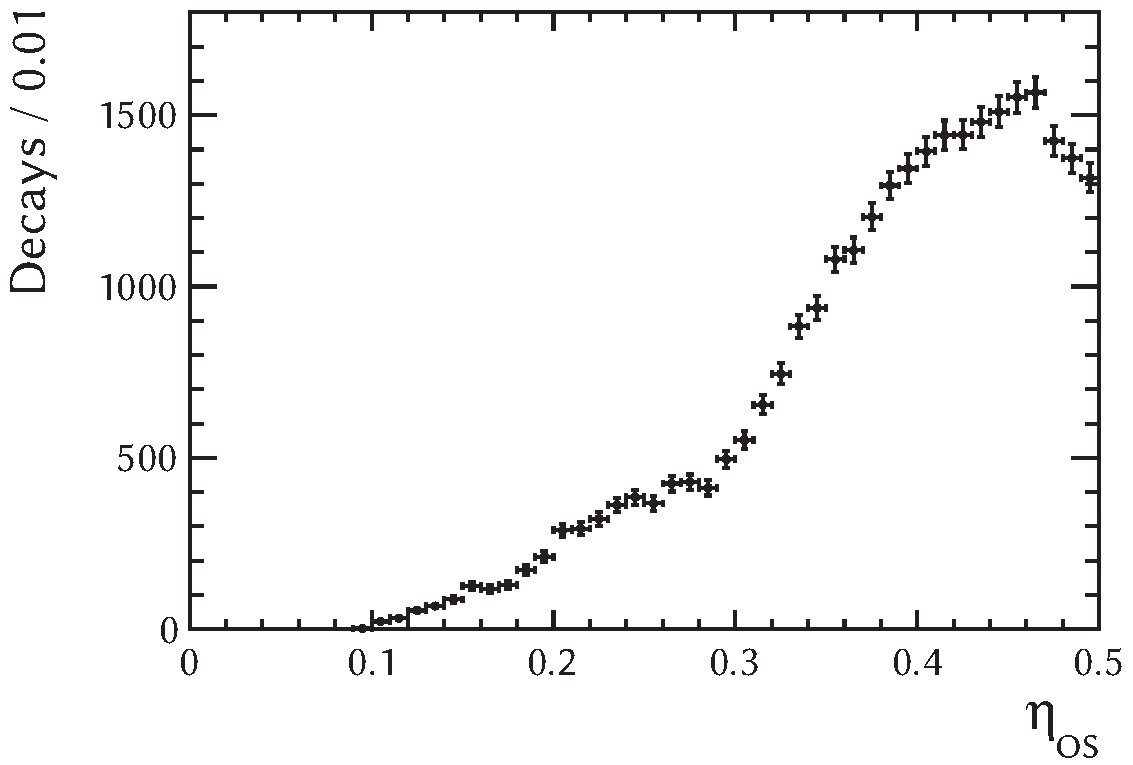
\includegraphics[width=\textwidth]{graphics/analysis/etaOS}
    \caption{}
    \label{fig:etaOS}
  \end{subfigure}%
  \hfill%
  \begin{subfigure}{0.49\textwidth}
    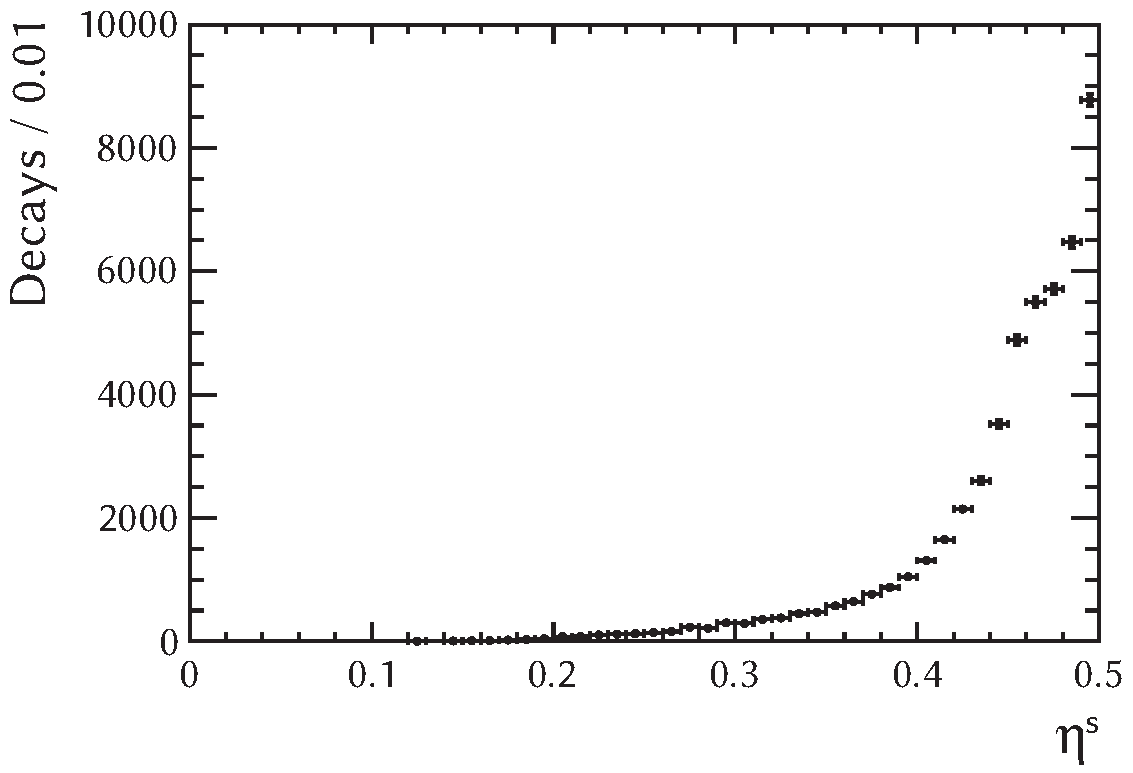
\includegraphics[width=\textwidth]{graphics/analysis/etaSS}
    \caption{}
    \label{fig:etaSS}
  \end{subfigure}
  \caption{Distribution of \BstoJpsiKK{} signal decays in the estimated wrong-tag probability
           for (a) opposite-side tagging and (b) same-side tagging.
           The contributions of untagged decays ($\etaTag$\textequiv0.5) are not shown.}
  \label{fig:etaDists}
\end{figure}

An individually normalized PDF is used for each tagging category to be insensitive to the fractions of decays in the categories, for which
there are no predictions. Since also the distributions in estimated wrong-tag probability are unpredicted, the PDFs are also made
conditional on this variable and normalized individually with respect to decay time and decay angles for each combination of $\etaOS$ and
$\etaSS$ values.

To reduce the sensitivity to \BsBsbar{} normalization asymmetries, the PDFs are also made conditional on the estimates of the $\Bs$
flavour, $\qtOS$ and $\qtSS$.
\textit{discuss why this reduces sensitivity on asymmetries}

\section{Simulation}
\label{sec:ana_sim}
\begin{itemize}
  \item \underline{briefly} discuss detector simulation
  \item toys: generate signal with model and background with real side-band data
  \item candidate weights and conditional observables in toys from fit dataset
\end{itemize}

Datasets of simulated decays are used to study the statistical precision of parameter estimates and the effect of the detector on
distributions of relevant variables. These data are generated using Monte Carlo methods, where the values of the variables that describe a
decay are drawn from the input distributions of those variables.

Two types of simulation are applied for this measurement. The first is a full simulation of the proton--proton collisions of the LHC, the
decays of particles that are produced, and the response of the LHCb detector to the resulting particles. These stages of the simulation are
performed separately for each simulated LHC event, generating values for variables that describe particles and detector components. The
resulting data are stored in the format of real detector data and are processed in the same way by applying trigger and selection
requirements. This type of simulation is applied to determine the contribution of resonant backgrounds (see
Section~\ref{subsec:ana_bkgSub_bkgSub}), the detector resolution (see Section~\ref{subsec:ana_bkgSub_bkgSub} for $\JpsiKK$ mass and
Section~\ref{subsec:ana_time_res} for decay time), and the detector acceptance (see Section~\ref{subsec:ana_time_acc} for decay time and
Section~\ref{sec:ana_angles} for decay angles).

In the second type of simulation the values of decay time and decay angles in \BstoJpsiKK{} decays are drawn from the PDF that is
constructed with the model discussed in Chapter~\ref{chap:pheno} and this chapter. All effects of $\Bs$ production, \BstoJpsiKK{} decay,
detection, reconstruction, and selection are then assumed to be described by this model, as in the fit of time and angles. This type of
simulation is applied to generate so called \emph{pseudo experiments}, each of which consists of a dataset that is equivalent to the
dataset obtained from the real experiment. Distributions of the parameter estimates in the final fit are obtained by performing the time
and angular analysis on each of the pseudo experiments. These distributions are used to determine the statistical uncertainty in the
parameter estimates (see Section~\ref{sec:result_paramEst}) and the effects of variations in the assumed model.


\chapter{Results}
\label{chap:result}

\section{Parameter Estimates}
\section{Systematic Errors}
\section{Unconstrained \texorpdfstring{$\Delms$}{Deltams}}
\section{Narrow \texorpdfstring{$\KK$}{KK}-Mass Window}
\section{Alternative Flavour-Tagging Schemes}
\subsection{Untagged Analysis}
\subsection{Analysis in Estimated Wrong-Tag Probability Bins}
\section{\texorpdfstring{\BsBsbar{}}{Bs0-Bs0bar} Asymmetries}


\makeatletter
\patchcmd{\@makechapterhead}{\@chapapp\space \thechapter}{\@chapapp}{}{}
\makeatother

\renewcommand{\thechapter}{C}
\renewcommand{\chaptermark}[1]{\markboth{Conclusions}{Conclusions}}
\renewcommand{\sectionmark}[1]{\markright{Conclusions}}
\chapter*{Conclusions}
\chaptermark{}

Figure~\ref{fig:phisDGsNew} shows the current status of $\phis$ and $\DGs$ measurements. It is an update of Figure~\ref{fig:phisDGs} in
Section~\ref{subsec:intro_Jpsiphi_decay}, which gives an overview of the status in the Spring of 2014, when only results with the 2011
dataset from LHCb were available. Results of the measurement presented in this thesis, which uses both the 2011 and 2012 LHCb datasets and
was published in \cite{LHCb-PAPER-2014-059}, are shown in combination with the results from measurements in the
\BstoJpsipipi~\cite{LHCb-PAPER-2014-019} and \BstoDspDsm~\cite{LHCb-PAPER-2014-051} decay channels. The other results in the figure are
from a new CMS measurement~\cite{CMS:2014jxa}, the updated \atlas{} measurement~\cite{Aad:2014cqa}, and the CDF~\cite{Aaltonen:2012ie} and
D0~\cite{Abazov:2011ry} measurements in the \BstoJpsiphi{} channel.
\begin{figure}[htb]
  \centering
  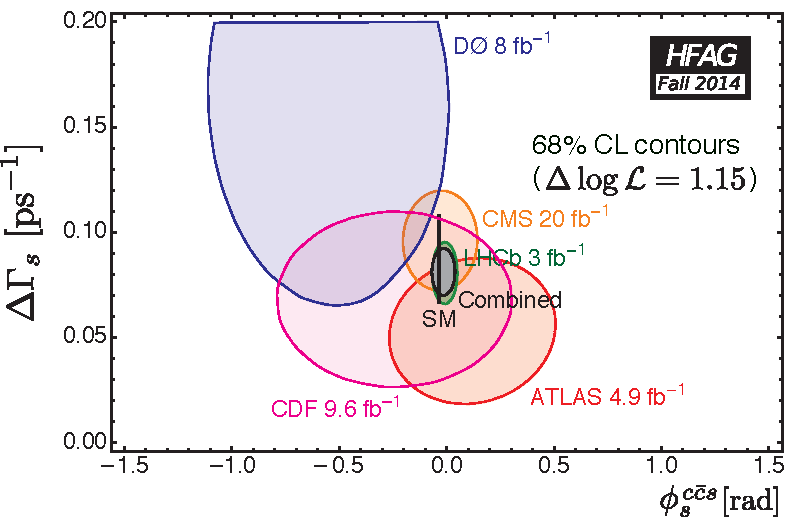
\includegraphics[width=\textwidth]{graphics/results/hfag_Fall2014_DGsphis-cmyk}
  \caption{Combination of $\phis$ (here represented as $\phisccs$) and $\DGs$ measurements by HFAG~\cite{Amhis:2012bh}.
           The estimates at 68\% confidence level (CL) by the different experiments are shown by the coloured contours.
           Note that the LHCb contour (green) is a combination of measurements in the
           \BstoJpsiphi{}, \BstoJpsipipi{}, and \BstoDspDsm{} decays.
           The combined 68\% confidence region is shown by the grey area and the Standard Model prediction by the vertical bar.}
  \label{fig:phisDGsNew}
\end{figure}

The objective of these measurements, as described in Sections~\ref{sec:intro_SM}--\ref{sec:intro_Jpsiphi}, is to test the Standard Model by
comparing the CP violation that is measured in $\btoccs$ transitions to the prediction obtained by interpreting other measurements within
the Standard Model framework. The current combined precision of the $\phis$ result is 0.04\unitsp{}rad, which is equal to the deviation of
the Standard Model prediction from zero. This precision is not yet sufficient to measure potential small deviations from the Standard
Model, but these measurements do rule out large contributions from non-Standard Model physics. As discussed in
Section~\ref{subsec:intro_Jpsiphi_decay}, both experimental and theoretical improvements are required for a more precise analysis of CP
violation in $\btoccs$ transitions.

At lowest order, the decays that are included in the combination of Figure~\ref{fig:phisDGsNew} are governed by a single tree-level
$\btoccs$ transition and CP violation is described by common $\phis$ and $\lamsAbs$ parameters. To compare a more precise measurement of CP
violation to its prediction in the Standard Model, higher order (penguin) contributions must be considered. These potentially yield CP
violation parameters with different values for each decay and each angular-momentum state contributing to the \BstoJpsiKK{} decay.

A close interplay between theory and experiment will be required to interpret a precise measurement of these CP-violation parameters.
Calculations of their values (see e.g. \cite{Liu:2013nea}) suffer from uncertainties in the strong interactions within the involved
hadrons. However, by exploiting approximate symmetries between different decays of $\Bd$ and $\Bs$ mesons, a framework of measurements
and calculations can be built to interpret the experimental results~\cite{Faller:2008gt,DeBruyn:2014oga}. Both precise measurements and
precise estimates of how the symmetries between different decays are broken are required for such an analysis.

In reference~\cite{DeBruyn:2014oga} it is proposed to use the interplay between the decays \BstoJpsiphi, \BstoJpsiKS, \BdtoJpsiKS, and
\BdtoJpsirho{} for an analysis of CP violation in $\btoccs$ and $\btoccd$ transitions. For both the \BstoJpsiphi{} and \BdtoJpsirho{}
decays measurements of CP violation per intermediate angular-momentum state is required in this framework. The results of the first
measurement in this format for the \BstoJpsiphi{} channel was presented in Chapter~\ref{chap:result} (see also
reference~\cite{LHCb-PAPER-2014-059}).

While the current CP-violation results are still compatible with both the Standard Model and no CP violation, it is expected that the
measurement with future LHCb data will start to distinguish between the Standard Model and other scenarios. With the final dataset of the
LHCb experiment an increase in statistical precision of roughly an order of magnitude is
expected~\cite{CERN-LHCC-2011-001,LHCB-PAPER-2012-031}.



\renewcommand{\chaptermark}[1]{\defaultchaptermark{#1}}
\renewcommand{\sectionmark}[1]{\defaultsectionmark{#1}}

\appendix
\renewcommand{\chaptermark}[1]{\markboth{Appendix. \ #1}{}}
\chapter{Angular Differential Decay Rate}
\label{chap:angularDecay}

%%%%%%%%%%%%%%%%%%%%%%%%%%%%
\section{Angular Amplitude}
\label{sec:angularDecay_amp}
%%%%%%%%%%%%%%%%%%%%%%%%%%%%

The dependence of the \BstoJpsiKK{} decay on the three decay angles, as described in Section~\ref{sec:pheno_angles}, can be derived within
the helicity formalism~\cite{Jacob:1959at,Chung:1971ri,*Richman:1984gh,*Kutschke:1996}. In this formalism the decay is described in terms
of three two-body decays; first the decay of the $\Bs$ into a $\Jpsi$ and a second intermediate particle, followed by the decay of the
$\Jpsi$ into a $\mumu$ pair and the decay of the second particle into a $\KK$ pair. The angular dependence arises from the rotations of the
spin vectors of the decaying particles into the momentum directions of the decaying particles.

\begin{figure}[p]
  \centering
  \resizebox{\textwidth}{!}{\input{graphics/angularDecay/helFormFrames.pdftex_t}}
  \caption{Helicity frames for the decay \BtoaPPbPP{} in (a) a general
    configuration where the coordinate systems in the $a$ and $b$ rest frames are aligned and (b)
    with the Jacob--Wick convention, in which the coordinate system in the $b$
    rest frame is rotated. A definition of the helicity angle $\phihel$ in the Jacob--Wick
    convention is shown in (c).}
  \label{fig:helFormFrames}
\end{figure}

A generalized form of the decay is shown in Figure~\ref{fig:helFormFrames}. The three coordinate systems in part (a) of the figure are
defined in the centre-of-mass frames of particles $B$, $a$, and $b$ in the decay \BtoaPPbPP. The spherical coordinates $\theta$ and
$\varphi$ specify the momentum direction of one of the particles in each two-body decay. The other particle, which is not shown in the
figure, has an opposite momentum.

The directions of the decay-product momenta define a \emph{helicity axis} for each of the three decays. The z axis of a particle coordinate
system lies along the helicity axis that is associated to the production of the particle. The momentum direction of one of the two
particles in a decay is chosen as the positive z direction, as depicted in Figure~\ref{fig:helFormFrames}a for particles $a$ and $b$.

The sum of the spin projections of the two particles in each decay along the helicity axis is given by the difference of the particle
helicities. Assuming the spin projection of the decaying particle in the z direction is known, the amplitude for the measuring the required
spin projection along the helicity axis is given by the complex conjugate of a \emph{Wigner D-matrix}, which is a function of three Euler
angles that specify the rotation of the spin projection from the z axis to the helicity axis.

The D-matrix for each of the two-body decays is expressed in terms of a real-valued d-matrix and two exponential functions as
\begin{equation}
  \label{eq:Ddef}
  \WD{j}{m}{n}{}(\varphi,\theta,\varphi') = e^{-im\varphi}\, \Wd{j}{m}{n}(\theta)\, e^{-in\varphi'}\ ,
\end{equation}
where $j$ is the spin of the decaying particle, $m$ the projection of the spin in the direction of the z axis, $n$ the projection of the
spin in the positive direction of the helicity axis. The Euler angles that specify the rotation of the spin projection are $\varphi$,
$\theta$, and $\varphi'$. The angles $\theta$ and $\varphi$ are equal to the spherical coordinates in the mother-particle rest frame, while
the angle $\varphi'$ rotates the coordinate system of a decay product around the helicity axis. In the \emph{Jacob-Wick} convention
$\varphi'$ is chosen to be equal to \tm$\varphi$, resulting in
\begin{equation}
  \label{eq:DdefJW}
  \WD{j}{m}{n}{}(\varphi,\theta,-\varphi) = \Wd{j}{m}{n}(\theta)\, e^{-i(m-n)\varphi}\ .
\end{equation}

A boost along the helicity axis does not affect the spin projections along this axis. Therefore, the projection of the spin of a decay
product along the helicity axis in the centre-of-mass frame of its production is equal to the spin projection in the z direction of the
coordinate system in its rest frame. As a result, this projection relates the spins the decays that are described in the two frames.

To define angles that are consistent with the helicity angles in Figure~\ref{fig:helAngles}, the coordinate system of particle $b$ is
rotated by 180\textdegree{} around the $\mathrm{y}_b$ axis, as shown in Figure~\ref{fig:helFormFrames}b. This operation introduces an
additional D-matrix, which represents the amplitude for a rotation with $\theta$\texteq$\pi$ and the other two Euler angles arbitrary, but
equal. The spin projection in the $\mathrm{z}_b$ direction goes from \tm$\lambda_b$ to \tp$\lambda_b$, where $\lambda_b$ is the helicity of
particle $b$ in the $B$ rest frame. Using the d-matrix property
$\Wd{j}{m}{n}(\pi)$\texteq$(\text{\tm1})^{j\text{\tm}n}\,\delta_{m,\text{\tm}n}$, this D-matrix can be written as
\begin{equation}
  \WD{j_b}{-\lambda_b}{\lambda_b}{*}(\gamma,\pi,\gamma)
      = e^{-i\lambda_b\gamma}\, \Wd{j_b}{-\lambda_b}{\lambda_b}(\theta)\, e^{+i\lambda_b\gamma}
      = (-1)^{j_b-\lambda_b}\ .
\end{equation}

Identifying the particles $P_1$ and $P_3$ with the particles $\Kp$ and $\lmu[+]$, respectively, the angle
$\theta_a$ corresponds to $\thetaK$ and the angle $\theta_b$ to $\thetal$. The angle $\phihel$ is given by the sum of $\varphi_a$ and
$\varphi_b$, as shown in Figure~\ref{fig:helFormFrames}c.

Combining the D-matrices for the three decays, the factor $\angAmp[]$ in Equation~\ref{eq:decayAmp} is given by
\begin{equation}
  \label{eq:angAmp}
  \begin{aligned}
    \angAmp[h] &=
         \sqrt{\tfrac{2j_B+1}{4\pi}\; \tfrac{2j_a^h+1}{4\pi}\; \tfrac{2j_b^h+1}{4\pi}}\\
         &\quad\times
         (-1)^{j_b^h-\lambda_b^h}\
         \WD{j_B}{\lambda_B}{\lambda_a^h-\lambda_b^h}{*}(\Omega_B)\
         \WD{j_a^h}{\lambda_a^h}{\lambda_1-\lambda_2}{*}(\Omega_a)\
         \WD{j_b^h}{\lambda_b^h}{\lambda_3-\lambda_4}{*}(\Omega_b)\ ,
  \end{aligned}
\end{equation}
where $\Omega_p$ is a shorthand notation for the set of Euler angles in the decay of particle $p$ and the factors
$\sqrt{\frac{2j+1}{4\pi}}$ are normalization factors for the two-particle states in the $B$, $a$, and $b$ decays. The index $h$ runs over
intermediate helicity states, for which the particles have definite helicities. The final expressions for helicity states will be combined
into expressions for the transversity states of Equation~\ref{eq:decayAmp}. Notice that the spins and helicities of particles $B$ and 1--4
do not depend on the intermediate state, since these particles are external and their spin state is, in principle, observable.

Concentrating only on the case where particle $B$ is a spinless particle, $j_B$, $\lambda_B$, and $\lambda_a$\textminus$\lambda_b$ are
equal to zero. As a result, the D-matrix corresponding to the $B$ decay reduces to $\WD{0}{0}{0}{*}$\texteq1, which makes the decay
independent of the orientation of the helicity axis with respect to the direction of the $B$ momentum. Introducing the notation
$\lambda_a$\texteq$\lambda_b$\textequiv$\lambda$, $\lambda_1$\textminus$\lambda_2$\textequiv$\alpha$, and
$\lambda_3$\textminus$\lambda_4$\textequiv$\beta$, Equation~\ref{eq:angAmp} reduces to
\begin{equation}
  \label{eq:angAmpRed}
  \begin{aligned}
    \angAmp[h] &=
         \frac{(-1)^{j_b^h-\lambda^h}}{(4\pi)^{3/2}} \sqrt{(2j_a^h+1)\, (2j_b^h+1)}\
         \WD{j_a^h}{\lambda^h}{\alpha}{*}(\Omega_a)\
         \WD{j_b^h}{\lambda^h}{\beta}{*}(\Omega_b)\ .
  \end{aligned}
\end{equation}

%%%%%%%%%%%%%%%%%%%%%%%%%%%%%%%%%%%
\section{Squared Angular Amplitude}
\label{sec:angularDecay_squareAmp}
%%%%%%%%%%%%%%%%%%%%%%%%%%%%%%%%%%%

With Equation~\ref{eq:angAmpRed} the products $\angAmp[h]^*\,\angAmp[h']^{\phantom{*}}$ that appear in Equation~\ref{eq:sqAmp} can be
expressed as
\begin{equation}
  \label{eq:angAmpSq}
  \begin{aligned}
    &\angAmp[h]^*\,\angAmp[h']^{\phantom{*}} \\
    &\qquad=\frac{(-1)^{j_b^h+j_b^{h'}+M^{hh'}-2\lambda^h}}{(4\pi)^{3}}
      \sqrt{(2j_a^h+1)\, (2j_a^{h'}+1)\, (2j_b^h+1)\, (2j_b^{h'}+1)}\\
      &\qquad\qquad\times
        \WD{j_a^h}{\lambda^h}{\alpha}{}(\Omega_a)\ \WD{j_a^{h'}}{\lambda^{h'}}{\alpha}{*}(\Omega_a)\
        \WD{j_b^h}{\lambda^h}{\beta}{}(\Omega_b)\ \WD{j_b^{h'}}{\lambda^{h'}}{\beta}{*}(\Omega_b)\ .
  \end{aligned}
\end{equation}
To evaluate the dependence between the D-matrices in this expression the following relations are applied:
\begin{subequations}
  \label{eq:Dprops}
  \begin{align}
    \WD{j}{m}{n}{*} &= (-1)^{m-n}\ \WD{j}{-m}{-n}{} \\
    \WD{j}{m}{n}\,\WD{j'}{m'}{n'}{}
      &= \sum_{J=|j-j'|}^{j+j'}
      \langle j\,m,\,j'\,m'|J\ m+m' \rangle \nonumber\\
      &\qquad\qquad\times
      \langle j\,n,\,j'\,n'|J\ n+n' \rangle\,
      \WD{J}{m+m'}{n+n'}{} \\
    \langle j\,m,\,j'\,m'|J\ M \rangle
      &= (-1)^{j-j'+M}\,\sqrt{2\,J+1}\
      \begin{pmatrix}
        \mss{j} & \mss{j'} & \mss{J} \\
        \mss{m} & \mss{m'} & \mss{-M}
      \end{pmatrix}
  \end{align}
\end{subequations}
where $\langle j\,m,\,j'\,m'|J\ M \rangle$ is a Clebsch-Gordan coefficient, which is related to the Wigner 3j symbol
$\begin{pmatrix} \mss{j} & \mss{j'} & \mss{J} \\ \mss{m} & \mss{m'} & \mss{-M} \end{pmatrix}$. The product of a D-matrix and a complex
conjugate D-matrix with equal indices $n$ can now be written as
\begin{equation}
  \label{eq:DDstar}
  \begin{aligned}
    \WD{j}{m}{n}{}\,\WD{j'}{m'}{n}{*}
    &= (-1)^{m'-n}\ \WD{j}{m}{n}{}\,\WD{j'}{-m'}{-n}{} \\
    &= (-1)^{m'-n} \sum_{J=|j-j'|}^{j+j'}
      \langle j\, m,\, j'\, -m' | J\ m-m' \rangle\\
      &\qquad\qquad\qquad\qquad\quad\times\langle j\,n,\,j'\,-n|J\,0 \rangle\
      \WD{J}{m-m'}{0}{} \\
    &= (-1)^{m-n} \sum_{J=|j-j'|}^{j+j'} \left(2J+1\right)\
      \begin{pmatrix}
        \mss{j} & \mss{j'} & \mss{J} \\
        \mss{m} & \mss{-m'} & \mss{-m+m'}
      \end{pmatrix}\\
      &\qquad\qquad\qquad\qquad\qquad\ \ \times
      \begin{pmatrix}
        \mss{j} & \mss{j'} & \mss{J} \\
        \mss{n} & \mss{-n} & \mss{0}
      \end{pmatrix}
      \WD{J}{m-m'}{0}{}\ .
  \end{aligned}
\end{equation}
With this expression the products of two D-matrices in Equation~\ref{eq:angAmpSq} that are functions of the same set of angles can be
substituted by a sum of single D-matrices. After this substitution and with the definition
$M^{hh'}$\textequiv$\lambda^h$\textminus$\lambda^{h'}$, the product $\angAmp[h]^*\,\angAmp[h']^{\phantom{*}}$ is given by
\begin{align}
  \label{eq:angAmpSqEval}
  &\angAmp[h]^*\,\angAmp[h']^{\phantom{*}} \nonumber\\*
  &\qquad=\frac{(-1)^{j_b^h+j_b^{h'}+M^{hh'}-\alpha-\beta}}{(4\pi)^{3}}
    \sqrt{(2j_a^h+1)\, (2j_a^{h'}+1)\, (2j_b^h+1)\, (2j_b^{h'}+1)} \nonumber\\
    &\qquad\quad \times
    \sum_{J_a^{hh'}=|j_a^h-j_a^{h'}|}^{j_a^h+j_a^{h'}} \left(2J_a^{hh'}+1\right)\
    \begin{pmatrix}
      \mss{j_a^h} & \mss{j_a^{h'}} & \mss{J_a^{hh'}} \\
      \mss{\lambda^h} & \mss{-\lambda^{h'}} & \mss{-M^{hh'}}
    \end{pmatrix}\
    \begin{pmatrix}
      \mss{j_a^h} & \mss{j_a^{h'}} & \mss{J_a^{hh'}} \\
      \mss{\alpha} & \mss{-\alpha} & \mss{0}
    \end{pmatrix} \nonumber\\
    &\qquad\quad \times
    \sum_{J_b^{hh'}=|j_b^h-j_b^{h'}|}^{j_b^h+j_b^{h'}} \left(2J_b^{hh'}+1\right)\
    \begin{pmatrix}
      \mss{j_b^h} & \mss{j_b^{h'}} & \mss{J_b^{hh'}} \\
      \mss{\lambda^h} & \mss{-\lambda^{h'}} & \mss{-M^{hh'}}
    \end{pmatrix}\
    \begin{pmatrix}
      \mss{j_b^h} & \mss{j_b^{h'}} & \mss{J_b^{hh'}} \\
      \mss{\beta} & \mss{-\beta} & \mss{0}
    \end{pmatrix} \nonumber\\*
    &\qquad\qquad\qquad\qquad\qquad\qquad\qquad\qquad\times
      \WD{J_a^{hh'}}{M^{hh'}}{0}{}(\Omega_a)\ \WD{J_b^{hh'}}{M^{hh'}}{0}{}(\Omega_b)\ .
\end{align}

Notice that the angular dependence is still written in terms of the sets of Euler angles corresponding to the decays of particles $a$ and
$b$, $\Omega_a$ and $\Omega_b$, respectively. The dependence on the helicity angles, $\thetaK$\textequiv$\theta_a$,
$\thetal$\textequiv$\theta_b$, and $\phihel$\textequiv$\varphi_a$\textplus$\varphi_b$, becomes apparent by expressing the product of
D-matrices in Equation~\ref{eq:angAmpSqEval} in terms of d-matrices and exponential functions (see Equation~\ref{eq:DdefJW}):
\begin{equation}
  \begin{aligned}
    \label{eq:Eultohel}
    &\WD{J_a^{hh'}}{M^{hh'}}{0}{}(\Omega_a)\ \WD{J_b^{hh'}}{M^{hh'}}{0}{}(\Omega_b) \\
    &\qquad= \Wd{J_a^{hh'}}{M^{hh'}}{0}(\theta_a)\ e^{-iM^{hh'}\varphi_a}\
             \Wd{J_b^{hh'}}{M^{hh'}}{0}(\theta_b)\ e^{-iM^{hh'}\varphi_b} \\
    &\qquad= \Wd{J_a^{hh'}}{M^{hh'}}{0}(\thetaK)\
             \Wd{J_b^{hh'}}{M^{hh'}}{0}(\thetal)\ e^{-iM^{hh'}\phihel}\\
    &\qquad= \sqrt{\frac{\left(J_a^{hh'}-M^{hh'}\right)!}{\left(J_a^{hh'}+M^{hh'}\right)!}\, \frac{4\pi}{2J_b^{hh'}+1}}\
             \aLp{J_a^{hh'}}{M^{hh'}}(\cthetaK)\,\sph{J_b^{hh'}}{M^{hh'}}{*}(\thetal,\phihel)\ .
  \end{aligned}
\end{equation}
The functions $\aLp{j}{m}(\cos\theta)$ and $\sph{j}{m}{}(\theta,\varphi)$ are associated Legendre polynomials and spherical harmonics,
respectively, which are defined by
\begin{subequations}
  \label{eq:PYdef}
  \begin{align}
    \Lp{j}(x) &\equiv \frac{1}{2^j j!} \frac{\ud^j}{\ud x^j} \left(x^2-1\right)^j \qquad \text{with } j\ge0 \\
    \aLp{j}{m}(x) &\equiv
      \left\{\begin{array}{cl}
        (-1)^m\,\left(1-x^2\right)^{\tfrac{1}{2}m}\,\frac{\ud^m}{\ud x^m}\Lp{j}(x) &\quad(m\ge0) \\
        \tfrac{(j-|m|)!}{(j+|m|)!}\,\left(1-x^2\right)^{\tfrac{1}{2}|m|}\,\frac{\ud^{|m|}}{\ud x^{|m|}}\Lp{j}(x) &\quad(m<0)
      \end{array}\right.\\
    \sph{j}{m}{}(\theta,\phi) &\equiv \sqrt{\tfrac{2j+1}{4\pi}\tfrac{(j-m)!}{(j+m)!}}\ \aLp{j}{m}(\cos\theta)\, e^{im\phi} \\
    \Wd{j}{m}{0}(\theta) &= \sqrt{\tfrac{(j-m)!}{(j+m)!}}\ \aLp{j}{m}(\cos\theta)\ .
  \end{align}
\end{subequations}

The angular functions that eventually appear in the expression of the differential decay rate are given by the real and imaginary parts of
the products $\angAmp[h]^*\,\angAmp[h']^{\phantom{*}}$. The only complex-valued factor on the right-hand side of
Equation~\ref{eq:angAmpSqEval} after substituting the expression for $\WD{J_a}{M}{0}{}(\Omega_a)\ \WD{J_b}{M}{0}{}(\Omega_b)$ from
Equation~\ref{eq:Eultohel} is the spherical harmonic $\sph{J_b}{M}{*}(\thetal,\phihel)$. Notice that this function is real valued if its
upper index is equal to zero:
\begin{equation}
    \sph{j}{0}{}(\theta,\phi) = \sqrt{\tfrac{2j+1}{4\pi}}\ \Lp{j}(\cos\theta)\ .
\end{equation}
Real-valued spherical harmonics are used in the angular functions, which are defined by
\begin{equation}
  \label{eq:realYdef}
  \rsph{j}{m}(\theta,\phi) = \left\{\begin{array}{cl}
                               Y_j^0(\theta,\phi) &\quad(m=0) \\[0.2em]
                               \sqrt{2}\ \Re[Y_j^m(\theta,\phi)] &\quad(m>0) \\[0.2em]
                               \sqrt{2}\ \Im[Y_j^{|m|}(\theta,\phi)] &\quad(m<0)
                             \end{array}\right.
\end{equation}

The squared amplitude in the helicity basis can be expressed in a form that is similar to Equation~\ref{eq:sqAmp}:
\begin{equation}
  \label{eq:sqAmpHel}
  \begin{aligned}
    |\mathcal{A}|^2
      &\propto \sum_h |H_h\,\angAmp[h]|^2 + \sum_{h\neq h'} \Re( H_h^*\,H_{h'}\, \angAmp[h]^*\,\angAmp[h'] ) \\
      &\propto \sum_h |H_h|^2\, |\angAmp[h]|^2 \\
        &\qquad + \sum_{h\neq h'} \Re(H_h^*\,H_{h'})\, \Re(\angAmp[h]^*\,\angAmp[h'])
                               - \Im(H_h^*\,H_{h'})\, \Im(\angAmp[h]^*\,\angAmp[h']) \ .
  \end{aligned}
\end{equation}
Terms in the second sum of Equation~\ref{eq:sqAmpHel} with $h$ and $h'$ swapped are identical, since $H_h^*\,H_{h'}\,
\angAmp[h]^*\,\angAmp[h']$ and $H_{h'}^*\,H_h\, \angAmp[h']^*\,\angAmp[h]$ are complex conjugates, which have identical real parts. The
sign of $M^{hh'}$\textequiv$\lambda^h$\textminus$\lambda^{h'}$ is opposite for these terms. Adding the two contributions for each of the
$h\leftrightarrow h'$ pairs, the angular functions in the helicity basis are given by
\begin{subequations}
  \label{eq:angFuncs}
  \begin{align}
    |\angAmp[h]|^2
      &\propto \aLp{J_a^{hh'}}{0}(\cthetaK)\,\sph{J_b^{hh'}}{0}{*}(\thetal,\phihel) \nonumber\\
      &\qquad= \aLp{J_a^{hh'}}{0}(\cthetaK)\, \rsph{J_b^{hh'}}{0}(\thetal,\phihel) \\
    2\,\Re(\angAmp[h]^*\,\angAmp[h'])
      &\propto 2\,\Re\!\left[ \aLp{J_a^{hh'}}{|M^{hh'}|}(\cthetaK)\,\sph{J_b^{hh'}}{|M^{hh'}|}{*}(\thetal,\phihel) \right] \nonumber\\
      &\qquad= \sqrt{2}\, \aLp{J_a^{hh'}}{|M^{hh'}|}(\cthetaK)\, \rsph{J_b^{hh'}}{|M^{hh'}|}(\thetal,\phihel) \\
    -2\,\Im(\angAmp[h]^*\,\angAmp[h'])
      &\propto -2\,\Im\!\left[ \aLp{J_a^{hh'}}{|M^{hh'}|}(\cthetaK)\,\sph{J_b^{hh'}}{|M^{hh'}|}{*}(\thetal,\phihel) \right] \nonumber\\
      &\qquad= \sqrt{2}\, \aLp{J_a^{hh'}}{|M^{hh'}|}(\cthetaK)\, \rsph{J_b^{hh'}}{-|M^{hh'}|}(\thetal,\phihel)
  \end{align}
\end{subequations}

%%%%%%%%%%%%%%%%%%%%%%%%%%%%%%%%%%%%%%%%%%%
\section{Angular Functions for \BstoJpsiKK}
\label{sec:angularDecay_functions}
%%%%%%%%%%%%%%%%%%%%%%%%%%%%%%%%%%%%%%%%%%%

Identifying particles $B$, $a$, and $b$ with the $\Bs$, the $\KK$ pair, and the $\Jpsi$, respectively, the angular dependence of the
\BstoJpsiKK{} decay can be derived from Equations~\ref{eq:angAmpSqEval}, \ref{eq:Eultohel}, \ref{eq:sqAmpHel}, and \ref{eq:angFuncs}.  As
discussed in Section~\ref{sec:pheno_decay}, the indices $h$ and $h'$ in Equation~\ref{eq:sqAmpHel} run over three \BstoJpsiphi{}
polarization states and one \BstoJpsiKK{} state where the $\KK$ pair is in an S-wave configuration.

Both the spins of the $\phimesalt$ and the $\Jpsi$ are equal to one ($j_a$\texteq$j_b$\texteq1), which results in sums over
$J_a$,\,$J_b$\texteq0,\,1,\,2 for each combination of the \BstoJpsiphi{} helicity states. The three states are given by the possible
$\phimesalt$ and $\Jpsi$ helicities: $\lambda$\texteq0 (``0''), $\lambda$\texteq\tp1 (``\tp''), and $\lambda$\texteq\tm1 (``\tm'').
Since the $\KK$ system has no orbital angular momentum for the $\KK$ S-wave (``S'') and the kaons are spinless, both $j_a$ and $\lambda$
are equal to zero for this state. The value of $J_a$ can only be zero for $h$\texteq$h'$\texteq{}S and one for $h$\textneq{}S and
$h'$\texteq{}S. Only one value for $|M^{hh'}|$\textequiv$|\lambda^h$\textminus$\lambda^{h'}|$ is possible for each combination of states,
varying from zero ($\lambda^h$\texteq$\lambda^{h'}$\texteq0) to two ($\lambda^h$\texteq\tm$\lambda^{h'}$\texteq1).

Kaons are spinless, which results in $\alpha$\texteq0 for the \BstoJpsiKK{} decay. The helicities of the muons from the $\Jpsi$ decay can
both be either \tp$\frac{\text{1}}{\text{2}}$ or \tm$\frac{\text{1}}{\text{2}}$, which gives the combinations $\beta$\textin\{0, \tpm1\}.
Since the $\mup$ and the $\mum$ are produced with opposite chirality, the case $\beta$\texteq0 requires the helicity of one of the muons to
be opposite to its chirality. These contributions are suppressed by a factor
$m_{\lmu[]}^2$/$m_{\mumu}^2$\textapprox\tenpow{-3}~\cite{Altmannshofer:2008dz}, where $m_{\lmu[]}$ is the muon mass and $m_{\mumu}$
the dimuon invariant mass, the latter of which is equal to the mass of the $\Jpsi$. For this reason only contributions with opposite
helicities are considered, for which $\beta$\texteq\tpm1.

\begin{table}[p]
  \centering
  \caption{Angular functions for the \BstoJpsiphi{} decay expressed in terms of associated Legendre polynomials and spherical harmonics
           in helicity angles. Functions are shown for $\beta$\texteq\tpm1.
           Top: functions in the helicity basis. Bottom: functions in the transversity basis.}
  \label{tab:angDistJpsiphiPY}
  \renewcommand{\arraystretch}{1.2}
  \begin{tabular}{cc}
    \hline
    amplitudes                             &
    %$hh'$                                  &
      $f(\Omega) \times 16\sqrt{\pi}$      \\
      %$f(\Omega) \times \tfrac{32\pi}{9}$  \\

    \hline\hline

    $\AmpSq[H]{0}$  &
    %00  &
      $4\, (P_0^0 + 2\, P_2^0)\, (Y_{0,\,0} - \tfrac{1}{\sqrt{5}}\, Y_{2,\,0})$  \\
      %$2\, \cos^2\thetaK\, \sin^2\thetal$  \\
    \hline

    $\AmpSq[H]{+}$  &
    %\tp\tp  &
      $2\, (P_0^0 - P_2^0)\, (2\, Y_{0,\,0} + \tfrac{1}{\sqrt{5}}\, Y_{2,\,0} \pm \sqrt{3}\, Y_{1,\,0})$  \\
      %$\tfrac{1}{2}\, \sin^2\thetaK\, (1 \pm \cos\thetal)^2$  \\
      &
      $\qquad\quad = P_2^2\, (2\, Y_{0,\,0} + \tfrac{1}{\sqrt{5}}\, Y_{2,\,0} \pm \sqrt{3}\, Y_{1,\,0})$  \\
    \hline

    $\AmpSq[H]{-}$  &
    %\tm{}\tm  &
      $2\, (P_0^0 - P_2^0)\, (2\, Y_{0,\,0} + \tfrac{1}{\sqrt{5}}\, Y_{2,\,0} \mp \sqrt{3}\, Y_{1,\,0})$  \\
      %$\tfrac{1}{2}\, \sin^2\thetaK\, (1 \mp \cos\thetal)^2$  \\
      &
      $\qquad\quad = P_2^2\, (2\, Y_{0,\,0} + \tfrac{1}{\sqrt{5}}\, Y_{2,\,0} \mp \sqrt{3}\, Y_{1,\,0})$  \\
    \hline

    $\ReAmp[H][H]{0}{+}$  &
    %0\tp{} ($\Re$)  &
      $+2\sqrt{\tfrac{3}{5}}\, P_2^1 (Y_{2,\,+1} \pm \sqrt{5}\, Y_{1,\,+1})$  \\
      %$\pm \sin2\thetaK\, \sin\thetal\, (1 \pm \cos\thetal) \cos\phihel$  \\
    \hline

    $\ImAmp[H][H]{0}{+}$  &
    %0\tp{} ($\Im$)  &
      $-2\sqrt{\tfrac{3}{5}}\, P_2^1 (Y_{2,\,-1} \pm \sqrt{5}\, Y_{1,\,-1})$  \\
      %$\mp \sin2\thetaK\, \sin\thetal\, (1 \pm \cos\thetal) \sin\phihel$  \\
    \hline

    $\ReAmp[H][H]{0}{-}$  &
    %0\tm{} ($\Re$)  &
      $+2\sqrt{\tfrac{3}{5}}\, P_2^1 (Y_{2,\,+1} \mp \sqrt{5}\, Y_{1,\,+1})$  \\
      %$\mp \sin2\thetaK\, \sin\thetal\, (1 \mp \cos\thetal) \cos\phihel$  \\
    \hline

    $\ImAmp[H][H]{0}{-}$  &
    %0\tm{} ($\Im$)  &
      $+2\sqrt{\tfrac{3}{5}}\, P_2^1 (Y_{2,\,-1} \mp \sqrt{5}\, Y_{1,\,-1})$  \\
      %$\mp \sin2\thetaK\, \sin\thetal\, (1 \mp \cos\thetal) \sin\phihel$  \\
    \hline

    $\ReAmp[H][H]{+}{-}$  &
    %\tp\tm{} ($\Re$)  &
      $-2\sqrt{\tfrac{3}{5}}\, P_2^2\, Y_{2,\,+2}$  \\
      %$-\sin^2\thetaK\, \sin^2\thetal\, \cos2\phihel$  \\
    \hline

    $\ImAmp[H][H]{+}{-}$  &
    %\tp\tm{} ($\Im$)  &
      $-2\sqrt{\tfrac{3}{5}}\, P_2^2\, Y_{2,\,-2}$  \\
      %$-\sin^2\thetaK\, \sin^2\thetal\, \sin2\phihel$  \\
    \hline\hline

    $\AmpSq{0}$  &
    %00  &
      $4\, (P_0^0 + 2\, P_2^0)\, (Y_{0,\,0} - \tfrac{1}{\sqrt{5}}\, Y_{2,\,0})$  \\
      %$2\, \cos^2\thetaK\, \sin^2\thetal$  \\
    \hline

    $\AmpSq{\parallel}$  &
    %$\parallel\parallel$  &
      $P_2^2\, (2\, Y_{0,\,0} + \tfrac{1}{\sqrt{5}}\, Y_{2,\,0} - \sqrt{\tfrac{3}{5}}\, Y_{2,\,+2})$  \\
      %$\sin^2\thetaK\, (1 - \sin^2\thetal\, \cos^2\phihel)$  \\
    \hline

    $\AmpSq{\perp}$  &
    %$\perp\perp$  &
      $P_2^2\, (2\, Y_{0,\,0} + \tfrac{1}{\sqrt{5}}\, Y_{2,\,0} + \sqrt{\tfrac{3}{5}}\, Y_{2,\,+2})$  \\
      %$\sin^2\thetaK\, (1 - \sin^2\thetal\, \sin^2\phihel)$  \\
    \hline

    $\ReAmp{0}{\parallel}$  &
    %0$\parallel$ ($\Re$)  &
      $+2\sqrt{2}\sqrt{\tfrac{3}{5}}\, P_2^1\, Y_{2,\,+1}$  \\
      %$+\frac{1}{\sqrt{2}}\, \sin2\thetaK\, \sin2\thetal\, \cos\phihel$  \\
    \hline

    $\ImAmp{0}{\parallel}$  &
    %0$\parallel$ ($\Im$)  &
      $\mp 2\sqrt{2}\;\sqrt{3}\, P_2^1\, Y_{1,\,-1}$  \\
      %$\mp \sqrt{2}\, \sin2\thetaK\, \sin\thetal\, \sin\phihel$  \\
    \hline

    $\ReAmp{0}{\perp}$  &
    %0$\perp$ ($\Re$)  &
      $\pm 2\sqrt{2}\;\sqrt{3}\, P_2^1\, Y_{1,\,+1}$  \\
      %$\pm \sqrt{2}\, \sin2\thetaK\, \sin\thetal\, \cos\phihel$  \\
    \hline

    $\ImAmp{0}{\perp}$  &
    %0$\perp$ ($\Im$)  &
      $-2\sqrt{2}\sqrt{\tfrac{3}{5}}\, P_2^1\, Y_{2,\,-1}$  \\
      %$-\frac{1}{\sqrt{2}}\, \sin2\thetaK\, \sin2\thetal\, \sin\phihel$  \\
    \hline

    $\ReAmp{\parallel}{\perp}$  &
    %$\parallel\perp$ ($\Re$)  &
      $\pm 2\sqrt{3}\, P_2^2\, Y_{1,\,0}$  \\
      %$\pm 2\, \sin^2\thetaK\, \cos\thetal$  \\
    \hline

    $\ImAmp{\parallel}{\perp}$  &
    %$\parallel\perp$ ($\Im$)  &
      $+2\sqrt{\tfrac{3}{5}}\, P_2^2\, Y_{2,\,-2}$  \\
      %$+\sin^2\thetaK\, \sin^2\thetal\, \sin2\phihel$  \\
    \hline
  \end{tabular}
\end{table}

\begin{table}[p]
  \centering
  \caption{Angular functions for the \BstoJpsiKK{} decay with a $\KK$ S-wave and the \BstoJpsiphi{} and $\KK$ S-wave interference
           expressed in terms of associated Legendre polynomials and spherical harmonics in helicity angles.
           Functions are shown for $\beta$\texteq\tpm1.
           Top: functions in the helicity basis. Bottom: functions in the transversity basis.}
  \renewcommand{\arraystretch}{1.2}
  \label{tab:angDistSWavePY}
  \begin{tabular}{cc}
    \hline
    amplitudes                             &
      $f(\Omega) \times 16\sqrt{\pi}$      \\
      %$f(\Omega) \times \tfrac{32\pi}{9}$  \\

    \hline\hline

    $\AmpSq[H]{{\text{S}}}$  &
      $4\, P_0^0\, (Y_{0,\,0} - \tfrac{1}{\sqrt{5}}\, Y_{2,\,0})$  \\
      %$\tfrac{2}{3}\, \sin^2\thetal$  \\
    \hline

    $\ReAmp[H][H]{0}{{\text{S}}}$  &
      $8\sqrt{3}\, P_1^0\, (Y_{0,\,0} - \tfrac{1}{\sqrt{5}}\, Y_{2,\,0})$  \\
      %$\tfrac{4}{3}\sqrt{3}\, \cos\thetaK\, \sin^2\thetal$  \\
    \hline

    $\ImAmp[H][H]{0}{{\text{S}}}$  &
      0  \\
      %0  \\
    \hline

    $\ReAmp[H][H]{+}{{\text{S}}}$  &
      $+6\, P_1^1\, (\tfrac{1}{\sqrt{5}}\, Y_{2,\,+1} \pm Y_{1,\,+1})$  \\
      %$\pm \tfrac{2}{3}\sqrt{3}\, \sin\thetaK\, \sin\thetal\, (1 \pm \cos\thetal)\, \cos\phihel$ \\
    \hline

    $\ImAmp[H][H]{+}{{\text{S}}}$  &
      $+6\, P_1^1\, (\tfrac{1}{\sqrt{5}}\, Y_{2,\,-1} \pm Y_{1,\,-1})$  \\
      %$\pm \tfrac{2}{3}\sqrt{3}\, \sin\thetaK\, \sin\thetal\, (1 \pm \cos\thetal)\, \sin\phihel$ \\
    \hline

    $\ReAmp[H][H]{-}{{\text{S}}}$  &
      $+6\, P_1^1\, (\tfrac{1}{\sqrt{5}}\, Y_{2,\,+1} \mp Y_{1,\,+1})$  \\
      %$\mp \tfrac{2}{3}\sqrt{3}\, \sin\thetaK\, \sin\thetal\, (1 \mp \cos\thetal)\, \cos\phihel$ \\
    \hline

    $\ImAmp[H][H]{-}{{\text{S}}}$  &
      $-6\, P_1^1\, (\tfrac{1}{\sqrt{5}}\, Y_{2,\,-1} \mp Y_{1,\,-1})$  \\
      %$\pm \tfrac{2}{3}\sqrt{3}\, \sin\thetaK\, \sin\thetal\, (1 \mp \cos\thetal)\, \sin\phihel$ \\
    \hline\hline

    $\AmpSq{{\text{S}}}$  &
      $4\, P_0^0\, (Y_{0,\,0} - \tfrac{1}{\sqrt{5}}\, Y_{2,\,0})$  \\
      %$\tfrac{2}{3}\, \sin^2\thetal$  \\
    \hline

    $\ReAmp{0}{{\text{S}}}$  &
      $8\sqrt{3}\, P_1^0\, (Y_{0,\,0} - \tfrac{1}{\sqrt{5}}\, Y_{2,\,0})$  \\
      %$\tfrac{4}{3}\sqrt{3}\, \cos\thetaK\, \sin^2\thetal$  \\
    \hline

    $\ImAmp{0}{{\text{S}}}$  &
      0  \\
      %0  \\
    \hline

    $\ReAmp{\parallel}{{\text{S}}}$  &
      $+6\sqrt{2}\tfrac{1}{\sqrt{5}}\, P_1^1\, Y_{2,\,+1}$  \\
      %$+\tfrac{1}{3}\sqrt{6}\, \sin\thetaK\, \sin2\thetal\, \cos\phihel$  \\
    \hline

    $\ImAmp{\parallel}{{\text{S}}}$  &
      $\pm 6\sqrt{2}\, P_1^1\, Y_{1,\,-1}$  \\
      %$\pm \tfrac{2}{3}\sqrt{6}\, \sin\thetaK\, \sin\thetal\, \sin\phihel$  \\
    \hline

    $\ReAmp{\perp}{{\text{S}}}$  &
      $\pm 6\sqrt{2}\, P_1^1\, Y_{1,\,+1}$  \\
      %$\pm \tfrac{2}{3}\sqrt{6}\, \sin\thetaK\, \sin\thetal\, \cos\phihel$  \\
    \hline

    $\ImAmp{\perp}{{\text{S}}}$  &
      $+6\sqrt{2}\tfrac{1}{\sqrt{5}}\, P_1^1\, Y_{2,\,-1}$  \\
      %$+\tfrac{1}{3}\sqrt{6}\, \sin\thetaK\, \sin2\thetal\, \sin\phihel$  \\
    \hline
  \end{tabular}
\end{table}

Evaluation of the angular functions for the combinations of the \BstoJpsiphi{} states leads to Table~\ref{tab:angDistJpsiphiPY}. The first
column of the table shows a combination of decay amplitudes and the second column the corresponding angular functions. The angular
functions for the $\KK$ S-wave and the interference between \BstoJpsiphi{} and the $\KK$ S-wave are listed in
Table~\ref{tab:angDistSWavePY}. All functions are multiplied by a factor 8$\pi^\text{2}$, which makes their integrals over all three angles
equal to either one or zero.

The differences between contributions from $\beta$\texteq\tpm1 are distinguished with \tpm{} and \tmp{} signs in the tables. Because the
decay of the $\Jpsi$ is not a weak process it conserves parity, which results in equal decay amplitudes for $\beta$\texteq\tp1 and
$\beta$\texteq\tm1. Since the muon helicities are not measured in the experiment, the two contributions are added, resulting in
cancellation of the terms with opposite sign.

The top halves of the tables show the angular amplitudes and functions in the helicity basis, while the bottom halves show the amplitudes
and functions in the transversity basis. For both bases helicity angles are used. The transversity functions are obtained by substituting
the helicity amplitudes ($H_0$, $H_+$, and $H_-$) by combinations of transversity amplitudes ($\Azero$, $\Apar$, and $\Aperp$), after which
the helicity functions can be combined into functions corresponding to the transversity amplitudes. The amplitude for the $\KK$ S-wave is
the same in both bases ($H_\text{S}$\texteq$\AS$). The substitution is given by~\cite{Dighe:1995pd}
\begin{equation}
  \label{eq:helToTransAmps}
  \begin{aligned}
    H_0   &= \Azero \\
    H_\pm &= \tfrac{1}{\sqrt{2}}(\Apar \pm \Aperp) \ .
  \end{aligned}
\end{equation}

Both Legendre polynomials and real-valued spherical harmonics can be expressed in terms of sines and cosines of the angles.
Tables~\ref{tab:angDistJpsiphiSinCos} and \ref{tab:angDistSWaveSinCos} show the angular functions in terms of sines and cosines that
correspond to the functions in Tables~\ref{tab:angDistJpsiphiPY} and \ref{tab:angDistSWavePY}, respectively.

\begin{table}[p]
  \centering
  \caption{Angular functions for the \BstoJpsiphi{} decay expressed in terms of sines and cosines in helicity angles.
           Functions are shown for $\beta$\texteq\tpm1.
           Top: functions in the helicity basis. Bottom: functions in the transversity basis.}
  \label{tab:angDistJpsiphiSinCos}
  \renewcommand{\arraystretch}{1.2}
  \begin{tabular}{cc}
    \hline
    amplitudes                             &
    %$hh'$                                  &
      %$f(\Omega) \times 16\sqrt{\pi}$      &
      $f(\Omega) \times \tfrac{32\pi}{9}$  \\

    \hline\hline

    $\AmpSq[H]{0}$  &
    %00  &
      %$4\, (P_0^0 + 2\, P_2^0)\, (Y_{0,\,0} - \tfrac{1}{\sqrt{5}}\, Y_{2,\,0})$  &
      $2\, \cos^2\thetaK\, \sin^2\thetal$  \\
    \hline

    $\AmpSq[H]{+}$  &
    %\tp\tp  &
      %$2\, (P_0^0 - P_2^0)\, (2\, Y_{0,\,0} + \tfrac{1}{\sqrt{5}}\, Y_{2,\,0} \pm \sqrt{3}\, Y_{1,\,0})$  &
      $\tfrac{1}{2}\, \sin^2\thetaK\, (1 \pm \cos\thetal)^2$  \\
    \hline

    $\AmpSq[H]{-}$  &
    %\tm{}\tm  &
      %$2\, (P_0^0 - P_2^0)\, (2\, Y_{0,\,0} + \tfrac{1}{\sqrt{5}}\, Y_{2,\,0} \mp \sqrt{3}\, Y_{1,\,0})$  &
      $\tfrac{1}{2}\, \sin^2\thetaK\, (1 \mp \cos\thetal)^2$  \\
    \hline

    $\ReAmp[H][H]{0}{+}$  &
    %0\tp{} ($\Re$)  &
      %$+2\sqrt{\tfrac{3}{5}}\, P_2^1 (Y_{2,\,+1} \pm \sqrt{5}\, Y_{1,\,+1})$  &
      $\pm \sin2\thetaK\, \sin\thetal\, (1 \pm \cos\thetal) \cos\phihel$  \\
    \hline

    $\ImAmp[H][H]{0}{+}$  &
    %0\tp{} ($\Im$)  &
      %$-2\sqrt{\tfrac{3}{5}}\, P_2^1 (Y_{2,\,-1} \pm \sqrt{5}\, Y_{1,\,-1})$  &
      $\mp \sin2\thetaK\, \sin\thetal\, (1 \pm \cos\thetal) \sin\phihel$  \\
    \hline

    $\ReAmp[H][H]{0}{-}$  &
    %0\tm{} ($\Re$)  &
      %$+2\sqrt{\tfrac{3}{5}}\, P_2^1 (Y_{2,\,+1} \mp \sqrt{5}\, Y_{1,\,+1})$  &
      $\mp \sin2\thetaK\, \sin\thetal\, (1 \mp \cos\thetal) \cos\phihel$  \\
    \hline

    $\ImAmp[H][H]{0}{-}$  &
    %0\tm{} ($\Im$)  &
      %$+2\sqrt{\tfrac{3}{5}}\, P_2^1 (Y_{2,\,-1} \mp \sqrt{5}\, Y_{1,\,-1})$  &
      $\mp \sin2\thetaK\, \sin\thetal\, (1 \mp \cos\thetal) \sin\phihel$  \\
    \hline

    $\ReAmp[H][H]{+}{-}$  &
    %\tp\tm{} ($\Re$)  &
      %$-2\sqrt{\tfrac{3}{5}}\, P_2^2\, Y_{2,\,+2}$  &
      $-\sin^2\thetaK\, \sin^2\thetal\, \cos2\phihel$  \\
    \hline

    $\ImAmp[H][H]{+}{-}$  &
    %\tp\tm{} ($\Im$)  &
      %$-2\sqrt{\tfrac{3}{5}}\, P_2^2\, Y_{2,\,-2}$  &
      $-\sin^2\thetaK\, \sin^2\thetal\, \sin2\phihel$  \\
    \hline\hline

    $\AmpSq{0}$  &
    %00  &
      %$4\, (P_0^0 + 2\, P_2^0)\, (Y_{0,\,0} - \tfrac{1}{\sqrt{5}}\, Y_{2,\,0})$  &
      $2\, \cos^2\thetaK\, \sin^2\thetal$  \\
    \hline

    $\AmpSq{\parallel}$  &
    %$\parallel\parallel$  &
      %$P_2^2\, (2\, Y_{0,\,0} + \tfrac{1}{\sqrt{5}}\, Y_{2,\,0} - \sqrt{\tfrac{3}{5}}\, Y_{2,\,+2})$  &
      $\sin^2\thetaK\, (1 - \sin^2\thetal\, \cos^2\phihel)$  \\
    \hline

    $\AmpSq{\perp}$  &
    %$\perp\perp$  &
      %$P_2^2\, (2\, Y_{0,\,0} + \tfrac{1}{\sqrt{5}}\, Y_{2,\,0} + \sqrt{\tfrac{3}{5}}\, Y_{2,\,+2})$  &
      $\sin^2\thetaK\, (1 - \sin^2\thetal\, \sin^2\phihel)$  \\
    \hline

    $\ReAmp{0}{\parallel}$  &
    %0$\parallel$ ($\Re$)  &
      %$+2\sqrt{2}\sqrt{\tfrac{3}{5}}\, P_2^1\, Y_{2,\,+1}$  &
      $+\frac{1}{\sqrt{2}}\, \sin2\thetaK\, \sin2\thetal\, \cos\phihel$  \\
    \hline

    $\ImAmp{0}{\parallel}$  &
    %0$\parallel$ ($\Im$)  &
      %$\mp 2\sqrt{2}\;\sqrt{3}\, P_2^1\, Y_{1,\,-1}$  &
      $\mp \sqrt{2}\, \sin2\thetaK\, \sin\thetal\, \sin\phihel$  \\
    \hline

    $\ReAmp{0}{\perp}$  &
    %0$\perp$ ($\Re$)  &
      %$\pm 2\sqrt{2}\;\sqrt{3}\, P_2^1\, Y_{1,\,+1}$  &
      $\pm \sqrt{2}\, \sin2\thetaK\, \sin\thetal\, \cos\phihel$  \\
    \hline

    $\ImAmp{0}{\perp}$  &
    %0$\perp$ ($\Im$)  &
      %$-2\sqrt{2}\sqrt{\tfrac{3}{5}}\, P_2^1\, Y_{2,\,-1}$  &
      $-\frac{1}{\sqrt{2}}\, \sin2\thetaK\, \sin2\thetal\, \sin\phihel$  \\
    \hline

    $\ReAmp{\parallel}{\perp}$  &
    %$\parallel\perp$ ($\Re$)  &
      %$\pm 2\sqrt{3}\, P_2^2\, Y_{1,\,0}$  &
      $\pm 2\, \sin^2\thetaK\, \cos\thetal$  \\
    \hline

    $\ImAmp{\parallel}{\perp}$  &
    %$\parallel\perp$ ($\Im$)  &
      %$+2\sqrt{\tfrac{3}{5}}\, P_2^2\, Y_{2,\,-2}$  &
      $+\sin^2\thetaK\, \sin^2\thetal\, \sin2\phihel$  \\
    \hline
  \end{tabular}
\end{table}

\begin{table}[p]
  \centering
  \caption{Angular functions for the \BstoJpsiKK{} decay with a $\KK$ S-wave and the \BstoJpsiphi{} and $\KK$ S-wave interference
           expressed in terms of sines and cosines in helicity angles. Functions are shown for $\beta$\texteq\tpm1.
           Top: functions in the helicity basis. Bottom: functions in the transversity basis.}
  \renewcommand{\arraystretch}{1.2}
  \label{tab:angDistSWaveSinCos}
  \begin{tabular}{cc}
    \hline
    amplitudes                              &
      %$f(\Omega) \times 16\sqrt{\pi}$      &
      $f(\Omega) \times \tfrac{32\pi}{9}$  \\

    \hline\hline

    $\AmpSq[H]{{\text{S}}}$  &
      %$4\, P_0^0\, (Y_{0,\,0} - \tfrac{1}{\sqrt{5}}\, Y_{2,\,0})$  &
      $\tfrac{2}{3}\, \sin^2\thetal$  \\
    \hline

    $\ReAmp[H][H]{0}{{\text{S}}}$  &
      %$8\sqrt{3}\, P_1^0\, (Y_{0,\,0} - \tfrac{1}{\sqrt{5}}\, Y_{2,\,0})$  &
      $\tfrac{4}{3}\sqrt{3}\, \cos\thetaK\, \sin^2\thetal$  \\
    \hline

    $\ImAmp[H][H]{0}{{\text{S}}}$  &
      %0  &
      0  \\
    \hline

    $\ReAmp[H][H]{+}{{\text{S}}}$  &
      %$+6\, P_1^1\, (\tfrac{1}{\sqrt{5}}\, Y_{2,\,+1} \pm Y_{1,\,+1})$  &
      $\pm \tfrac{2}{3}\sqrt{3}\, \sin\thetaK\, \sin\thetal\, (1 \pm \cos\thetal)\, \cos\phihel$ \\
    \hline

    $\ImAmp[H][H]{+}{{\text{S}}}$  &
      %$+6\, P_1^1\, (\tfrac{1}{\sqrt{5}}\, Y_{2,\,-1} \pm Y_{1,\,-1})$  &
      $\pm \tfrac{2}{3}\sqrt{3}\, \sin\thetaK\, \sin\thetal\, (1 \pm \cos\thetal)\, \sin\phihel$ \\
    \hline

    $\ReAmp[H][H]{-}{{\text{S}}}$  &
      %$+6\, P_1^1\, (\tfrac{1}{\sqrt{5}}\, Y_{2,\,+1} \mp Y_{1,\,+1})$  &
      $\mp \tfrac{2}{3}\sqrt{3}\, \sin\thetaK\, \sin\thetal\, (1 \mp \cos\thetal)\, \cos\phihel$ \\
    \hline

    $\ImAmp[H][H]{-}{{\text{S}}}$  &
      %$-6\, P_1^1\, (\tfrac{1}{\sqrt{5}}\, Y_{2,\,-1} \mp Y_{1,\,-1})$  &
      $\pm \tfrac{2}{3}\sqrt{3}\, \sin\thetaK\, \sin\thetal\, (1 \mp \cos\thetal)\, \sin\phihel$ \\
    \hline\hline

    $\AmpSq{{\text{S}}}$  &
      %$4\, P_0^0\, (Y_{0,\,0} - \tfrac{1}{\sqrt{5}}\, Y_{2,\,0})$  &
      $\tfrac{2}{3}\, \sin^2\thetal$  \\
    \hline

    $\ReAmp{0}{{\text{S}}}$  &
      %$8\sqrt{3}\, P_1^0\, (Y_{0,\,0} - \tfrac{1}{\sqrt{5}}\, Y_{2,\,0})$  &
      $\tfrac{4}{3}\sqrt{3}\, \cos\thetaK\, \sin^2\thetal$  \\
    \hline

    $\ImAmp{0}{{\text{S}}}$  &
      %0  &
      0  \\
    \hline

    $\ReAmp{\parallel}{{\text{S}}}$  &
      %$+6\sqrt{2}\tfrac{1}{\sqrt{5}}\, P_1^1\, Y_{2,\,+1}$  &
      $+\tfrac{1}{3}\sqrt{6}\, \sin\thetaK\, \sin2\thetal\, \cos\phihel$  \\
    \hline

    $\ImAmp{\parallel}{{\text{S}}}$  &
      %$\pm 6\sqrt{2}\, P_1^1\, Y_{1,\,-1}$  &
      $\pm \tfrac{2}{3}\sqrt{6}\, \sin\thetaK\, \sin\thetal\, \sin\phihel$  \\
    \hline

    $\ReAmp{\perp}{{\text{S}}}$  &
      %$\pm 6\sqrt{2}\, P_1^1\, Y_{1,\,+1}$  &
      $\pm \tfrac{2}{3}\sqrt{6}\, \sin\thetaK\, \sin\thetal\, \cos\phihel$  \\
    \hline

    $\ImAmp{\perp}{{\text{S}}}$  &
      %$+6\sqrt{2}\tfrac{1}{\sqrt{5}}\, P_1^1\, Y_{2,\,-1}$  &
      $+\tfrac{1}{3}\sqrt{6}\, \sin\thetaK\, \sin2\thetal\, \sin\phihel$  \\
    \hline
  \end{tabular}
\end{table}

%\chapter{Systematics}
\label{chap:syst}

%%%%%%%%%%%%%%%%%%%%%
\section{Mass model}
\label{sec:syst_mass}
%%%%%%%%%%%%%%%%%%%%%

In the analysis of the decay-time and decay-angle distributions a set of fixed event weights is used to statistically separate signal and
background contributions (see Section~\ref{sec:ana_bkgSub}). The weights are based on the estimates of the signal and background
contributions to the $\JpsiKK$-mass distribution. Uncertainties in the mass model are propagated to the time and angular analysis by
evaluating the effects of different sets of weights on the final parameter estimates.

%%%%%%%%%%%%%%%%%%%%%%%%%%%%%%%%%%%
\subsection{Reflection backgrounds}
\label{subsec:syst_mass_peaking}
%%%%%%%%%%%%%%%%%%%%%%%%%%%%%%%%%%%

Reflection backgrounds from \BdtoJpsiKst{} and \LbtoJpsipK{} are subtracted by injecting simulated events with negative weights into the
data sample that is used for analysis. Two types of uncertainties arise from this procedure: uncertainties in the estimates of the numbers
of background events that affect the \BstoJpsiKK{} analysis and uncertainties in the relevant distributions of the reflection backgrounds.

A systematic uncertainty for the numbers of background events is estimated by changing the subtracted background yields by one standard
deviation. The (absolute) variations resulting from an upward and a downward fluctuation are averaged. The yields of all background
components are varied simultaneously.

The distributions of the decay angles and tagging variables of simulated background events are reweighted to make them match the
distributions in \BdtoJpsiKst{} and \LbtoJpsipK{} data as closely as possible. Since the results of this procedure are not expected to be
perfect, the difference in results with datasets containing reweighted and not reweighted distributions is taken as a systematic
uncertainty.

As a check, the analysis is also performed without subtracting the reflection backgrounds. The result is not used for evaluation of the
systematic uncertainties.

Results with the different datasets are shown in Tables~\ref{tab:syst_mass_peaking_phi} to \ref{tab:syst_mass_peaking_polarDep} for the
three different time and angular models. Only the differences with the nominal results (see Section~\ref{sec:result_paramEst}) are shown.
The resulting systematic uncertainties are shown in the last column.

\begin{table}[htbp]
  \centering
  \caption{Deviations in parameter estimates from the nominal results with the model with $\lamsAbs\equiv1$ for different schemes of
           subtracting reflection backgrounds.
           Differences with the nominal result are given in fractions of the statistical uncertainties. The resulting systematic
           uncertainty in the last column is obtained by taking the average of the yield-variation uncertainties and adding the reweighting
           uncertainty in quadrature. The absolute systematic is given in brackets.}
  \label{tab:syst_mass_peaking_phi}
  \begin{tabular}{lllllll}
    \hline
    par.            &  no sub.    &  yield--  &  yield+   &  no rew.  &  \multicolumn{2}{l}{systematic (abs.)}  \\
    \hline
    $\phis$         &  --0.041    &  --0.025  &   +0.025  &  --0.021  &  0.033  &  (0.0015)                     \\
    \hline
    $\Gs$           &   +0.000    &  --0.013  &   +0.016  &  --0.012  &  0.019  &  (0.000058)                   \\
    $\DGs$          &  --0.069    &  --0.007  &   +0.013  &  --0.046  &  0.047  &  (0.00043)                    \\
    $\Dms$          &   +0.086    &   +0.022  &  --0.020  &  --0.004  &  0.021  &  (0.0013)                     \\
    \hline
    $\magzeroSq$    &  --0.251    &  --0.007  &   +0.008  &  --0.072  &  0.072  &  (0.00025)                    \\
    $\magperpSq$    &   +0.180    &   +0.008  &  --0.003  &   +0.080  &  0.080  &  (0.00039)                    \\
    $\FS[1]$        &  --0.271    &  --0.043  &   +0.039  &   +0.070  &  0.081  &  (0.0044)                     \\
    $\FS[2]$        &   +0.070    &   +0.019  &  --0.011  &   +0.023  &  0.027  &  (0.00049)                    \\
    $\FS[3]$        &  --0.129    &  --0.019  &   +0.021  &  --0.010  &  0.022  &  (0.00015)                    \\
    $\FS[4]$        &  --0.084    &  --0.002  &   +0.005  &   +0.024  &  0.024  &  (0.00014)                    \\
    $\FS[5]$        &   +0.232    &   +0.025  &  --0.023  &   +0.023  &  0.033  &  (0.00054)                    \\
    $\FS[6]$        &  --0.140    &  --0.036  &   +0.039  &   +0.185  &  0.19   &  (0.0048)                     \\
    \hline
    $\delparzero$   &   +0.016    &   +0.020  &  --0.014  &  --0.195  &  0.20   &  (0.024)                      \\
    $\delperpzero$  &   +0.065    &   +0.029  &  --0.034  &  --0.088  &  0.093  &  (0.015)                      \\
    $\delSperp[1]$  &  --0.055    &  --0.025  &   +0.023  &   +0.117  &  0.12   &  (0.024)                      \\
    $\delSperp[2]$  &   +0.302    &   +0.036  &  --0.044  &   +0.105  &  0.11   &  (0.032)                      \\
    $\delSperp[3]$  &   +0.083    &   +0.011  &  --0.008  &  --0.040  &  0.041  &  (0.0094)                     \\
    $\delSperp[4]$  &  --0.058    &  --0.002  &  --0.000  &   +0.019  &  0.019  &  (0.0041)                     \\
    $\delSperp[5]$  &   +0.106    &   +0.007  &  --0.008  &  --0.100  &  0.10   &  (0.018)                      \\
    $\delSperp[6]$  &  --0.051    &   +0.003  &  --0.002  &   +0.047  &  0.047  &  (0.0065)                     \\
    \hline
  \end{tabular}
\end{table}

\begin{table}[htbp]
  \centering
  \caption{Deviations in parameter estimates from the nominal results with the model with a free $\lamsAbs$ for different schemes of
           subtracting reflection backgrounds.
           Differences with the nominal result are given in fractions of the statistical uncertainties. The resulting systematic
           uncertainty in the last column is obtained by taking the average of the yield-variation uncertainties and adding the reweighting
           uncertainty in quadrature. The absolute systematic is given in brackets.}
  \label{tab:syst_mass_peaking_lamb_phi}
  \begin{tabular}{lllllll}
    \hline
    par.            &  no sub.    &  yield--  &  yield+   &  no rew.  &  \multicolumn{2}{l}{systematic (abs.)}  \\
    \hline
    $\phis$         &  --0.026    &  --0.022  &   +0.020  &  --0.023  &  0.031  &  (0.0015)                     \\
    $\lamsAbs$      &  --0.010    &   +0.010  &  --0.009  &   +0.147  &  0.15   &  (0.0028)                     \\
    \hline
    $\Gs$           &  --0.022    &  --0.012  &   +0.015  &  --0.047  &  0.049  &  (0.00015)                    \\
    $\DGs$          &  --0.056    &  --0.005  &   +0.004  &  --0.028  &  0.028  &  (0.00026)                    \\
    $\Dms$          &   +0.057    &   +0.007  &  --0.005  &  --0.027  &  0.028  &  (0.0016)                     \\
    \hline
    $\magzeroSq$    &  --0.238    &  --0.003  &   +0.004  &  --0.054  &  0.054  &  (0.00019)                    \\
    $\magperpSq$    &   +0.165    &   +0.008  &  --0.007  &   +0.068  &  0.068  &  (0.00034)                    \\
    $\FS[1]$        &  --0.277    &  --0.045  &   +0.039  &   +0.057  &  0.071  &  (0.0038)                     \\
    $\FS[2]$        &   +0.095    &   +0.004  &  --0.002  &   +0.038  &  0.038  &  (0.00067)                    \\
    $\FS[3]$        &  --0.111    &  --0.009  &   +0.009  &   +0.001  &  0.009  &  (0.00006)                    \\
    $\FS[4]$        &  --0.100    &  --0.003  &   +0.003  &  --0.004  &  0.005  &  (0.00003)                    \\
    $\FS[5]$        &   +0.216    &   +0.018  &  --0.018  &  --0.006  &  0.019  &  (0.00029)                    \\
    $\FS[6]$        &  --0.154    &  --0.030  &   +0.031  &   +0.184  &  0.19   &  (0.0048)                     \\
    \hline
    $\delparzero$   &   +0.037    &   +0.017  &  --0.014  &  --0.188  &  0.19   &  (0.023)                      \\
    $\delperpzero$  &   +0.015    &   +0.012  &  --0.010  &  --0.126  &  0.13   &  (0.018)                      \\
    $\delSperp[1]$  &  --0.031    &  --0.020  &   +0.018  &   +0.121  &  0.12   &  (0.024)                      \\
    $\delSperp[2]$  &   +0.335    &   +0.029  &  --0.030  &   +0.128  &  0.13   &  (0.037)                      \\
    $\delSperp[3]$  &   +0.058    &   +0.001  &  --0.001  &  --0.055  &  0.055  &  (0.012)                      \\
    $\delSperp[4]$  &  --0.056    &   +0.002  &  --0.002  &   +0.001  &  0.002  &  (0.0004)                     \\
    $\delSperp[5]$  &   +0.077    &  --0.003  &   +0.004  &  --0.142  &  0.14   &  (0.022)                      \\
    $\delSperp[6]$  &  --0.060    &   +0.011  &  --0.009  &   +0.041  &  0.042  &  (0.0059)                     \\
    \hline
  \end{tabular}
\end{table}

\begin{table}[htbp]
  \centering
  \caption{Deviations in parameter estimates from the nominal results with the model with polarization-dependent CP violation for
           different schemes of subtracting reflection backgrounds.
           Differences with the nominal result are given in fractions of the statistical uncertainties. The resulting systematic
           uncertainty in the last column is obtained by taking the average of the yield-variation uncertainties and adding the reweighting
           uncertainty in quadrature. The absolute systematic is given in brackets.}
  \label{tab:syst_mass_peaking_polarDep}
  \begin{tabular}{lllllll}
    \hline
    par.            &  no sub.    &  yield--  &  yield+   &  no rew.  &  \multicolumn{2}{l}{systematic (abs.)}  \\
    \hline
    $\phisav$       &  --0.077    &  --0.024  &   +0.022  &  --0.053  &  0.058  &  (0.0029)                     \\
    $\Delphispara$  &   +0.030    &   +0.015  &  --0.014  &   +0.020  &  0.025  &  (0.0011)                     \\
    $\Delphisperpp$ &  --0.033    &  --0.001  &   +0.002  &  --0.032  &  0.032  &  (0.00092)                    \\
    $\DelphisS$     &   +0.009    &   +0.016  &  --0.013  &  --0.136  &  0.14   &  (0.0085)                     \\
    \hline
    $\Csav$         &   +0.094    &   +0.000  &  --0.001  &   +0.029  &  0.029  &  (0.0011)                     \\
    $\DelCspara$    &   +0.120    &   +0.008  &  --0.006  &  --0.062  &  0.062  &  (0.0076)                     \\
    $\DelCsperp$    &   +0.111    &   +0.015  &  --0.014  &  --0.021  &  0.026  &  (0.0041)                     \\
    $\CsavS$        &  --0.134    &  --0.031  &   +0.030  &  --0.104  &  0.11   &  (0.0035)                     \\
    \hline
    $\Gs$           &  --0.008    &  --0.011  &   +0.017  &  --0.043  &  0.045  &  (0.00014)                    \\
    $\DGs$          &  --0.066    &  --0.004  &   +0.004  &  --0.022  &  0.022  &  (0.00020)                    \\
    $\Dms$          &   +0.121    &   +0.009  &  --0.007  &   +0.021  &  0.022  &  (0.0014)                     \\
    \hline
    $\magzeroAvSq$  &  --0.248    &  --0.003  &   +0.004  &  --0.048  &  0.048  &  (0.00017)                    \\
    $\magperpAvSq$  &   +0.173    &   +0.008  &  --0.008  &   +0.059  &  0.060  &  (0.00029)                    \\
    $\FSAv[1]$      &  --0.275    &  --0.044  &   +0.038  &   +0.062  &  0.074  &  (0.0040)                     \\
    $\FSAv[2]$      &   +0.105    &   +0.001  &  --0.000  &   +0.054  &  0.054  &  (0.00095)                    \\
    $\FSAv[3]$      &  --0.060    &  --0.006  &   +0.006  &   +0.008  &  0.010  &  (0.000066)                   \\
    $\FSAv[4]$      &  --0.099    &  --0.003  &   +0.003  &   +0.014  &  0.014  &  (0.000081)                   \\
    $\FSAv[5]$      &   +0.204    &   +0.016  &  --0.015  &   +0.002  &  0.016  &  (0.00024)                    \\
    $\FSAv[6]$      &  --0.146    &  --0.032  &   +0.032  &   +0.182  &  0.19   &  (0.0047)                     \\
    \hline
    $\delparzero$   &   +0.048    &   +0.019  &  --0.016  &  --0.178  &  0.18   &  (0.024)                      \\
    $\delperpzero$  &   +0.081    &   +0.012  &  --0.010  &  --0.064  &  0.065  &  (0.011)                      \\
    $\delSperp[1]$  &  --0.021    &  --0.017  &   +0.016  &   +0.096  &  0.097  &  (0.020)                      \\
    $\delSperp[2]$  &   +0.353    &   +0.033  &  --0.033  &   +0.133  &  0.14   &  (0.042)                      \\
    $\delSperp[3]$  &   +0.013    &   +0.000  &  --0.000  &  --0.077  &  0.077  &  (0.019)                      \\
    $\delSperp[4]$  &  --0.055    &   +0.002  &  --0.002  &   +0.001  &  0.002  &  (0.0004)                     \\
    $\delSperp[5]$  &   +0.073    &  --0.005  &   +0.005  &  --0.146  &  0.15   &  (0.023)                      \\
    $\delSperp[6]$  &  --0.050    &   +0.013  &  --0.010  &   +0.011  &  0.016  &  (0.0023)                     \\
    \hline
  \end{tabular}
\end{table}


%%%%%%%%%%%%%%%%%%%%%%%%%%%%%%%%%%%%%%%%%%%%%%%%%%%%%%%%%%%%%
\subsection{Signal and combinatorial background: statistical}
\label{subsec:syst_mass_stat}
%%%%%%%%%%%%%%%%%%%%%%%%%%%%%%%%%%%%%%%%%%%%%%%%%%%%%%%%%%%%%

Statistical uncertainties in the $\JpsiKK$-mass models of the signal and the combinatorial background are propagated by repeating the time
and angular fit with different sets of signal weights. The sets of weights are obtained by calculating \sweight[s] with different sets of
mass-model parameters, which are generated according to a multivariate-Gaussian distribution using the means and covariances from the mass
fit.

Tables~\ref{tab:syst_mass_stat_lamb_phi} and \ref{tab:syst_mass_stat_polarDep} show the results of fits to five thousand datasets with
varying signal weights. The square root of the mean squared difference with the nominal result is taken as a systematic uncertainty for
each parameter.

\begin{table}[htbp]
  \centering
  \caption{Deviations in parameter estimates from the nominal results with the $\lamsAbs\equiv1$ and free $\lamsAbs$ models for five
           thousand datasets with varying signal weights.
           The square root of the mean squared difference with the nominal result is shown for each parameter, both as a fraction of the
           statistical uncertainty and as an absolute value (in brackets).}
  \label{tab:syst_mass_stat_lamb_phi}
  \begin{tabular}{lllll}
    \hline
    par.            &  \multicolumn{2}{l}{deviation $\lamsAbs\equiv1$}  &  \multicolumn{2}{l}{deviation free $\lamsAbs$}  \\
    \hline
    $\phis$         &  0.004  &  (0.00019)                              &  0.004  &  (0.00021)                            \\
    $\lamsAbs$      &  --     &  --                                     &  0.005  &  (0.000088)                           \\
    \hline
    $\Gs$           &  0.044  &  (0.00014~\invps)                       &  0.041  &  (0.00013~\invps)                     \\
    $\DGs$          &  0.012  &  (0.00011~\invps)                       &  0.009  &  (0.000080~\invps)                    \\
    $\Dms$          &  0.009  &  (0.00051~\invps)                       &  0.005  &  (0.00031~\invps)                     \\
    \hline
    $\magzeroSq$    &  0.027  &  (0.000094)                             &  0.020  &  (0.000071)                           \\
    $\magperpSq$    &  0.014  &  (0.000070)                             &  0.009  &  (0.000043)                           \\
    $\FS[1]$        &  0.14   &  (0.0078)                               &  0.15   &  (0.0080)                             \\
    $\FS[2]$        &  0.042  &  (0.00075)                              &  0.032  &  (0.00056)                            \\
    $\FS[3]$        &  0.010  &  (0.000066)                             &  0.006  &  (0.000039)                           \\
    $\FS[4]$        &  0.013  &  (0.000076)                             &  0.009  &  (0.000055)                           \\
    $\FS[5]$        &  0.032  &  (0.00052)                              &  0.024  &  (0.00037)                            \\
    $\FS[6]$        &  0.047  &  (0.0012)                               &  0.046  &  (0.0012)                             \\
    \hline
    $\delparzero$   &  0.018  &  (0.0023)                               &  0.014  &  (0.0018)                             \\
    $\delperpzero$  &  0.012  &  (0.0019)                               &  0.008  &  (0.0011)                             \\
    $\delSperp[1]$  &  0.028  &  (0.0055)                               &  0.023  &  (0.0045)                             \\
    $\delSperp[2]$  &  0.022  &  (0.0064)                               &  0.012  &  (0.0035)                             \\
    $\delSperp[3]$  &  0.007  &  (0.0016)                               &  0.002  &  (0.00050)                            \\
    $\delSperp[4]$  &  0.009  &  (0.0020)                               &  0.005  &  (0.00085)                            \\
    $\delSperp[5]$  &  0.016  &  (0.0028)                               &  0.007  &  (0.0011)                             \\
    $\delSperp[6]$  &  0.009  &  (0.0013)                               &  0.010  &  (0.0014)                             \\
    \hline
  \end{tabular}
\end{table}

\begin{table}[htbp]
  \centering
  \caption{Deviations in parameter estimates from the nominal results with the model with polarization-dependent CP violation for five
           thousand datasets with varying signal weights.
           The square root of the mean squared difference with the nominal result is shown for each parameter, both as a fraction of the
           statistical uncertainty and as an absolute value (in brackets).}
  \label{tab:syst_mass_stat_polarDep}
  \begin{tabular}{lll}
    \hline
    par.            &  \multicolumn{2}{l}{deviation polar. dep.}  \\
    \hline
    $\phisav$       &  0.004  &  (0.00023)                        \\
    $\Delphispara$  &  0.003  &  (0.00014)                        \\
    $\Delphisperpp$ &  0.008  &  (0.00022)                        \\
    $\DelphisS$     &  0.010  &  (0.00064)                        \\
    \hline
    $\Csav$         &  0.005  &  (0.00020)                        \\
    $\DelCspara$    &  0.005  &  (0.00066)                        \\
    $\DelCsperp$    &  0.005  &  (0.00075)                        \\
    $\CsavS$        &  0.007  &  (0.00024)                        \\
    \hline
    $\Gs$           &  0.041  &  (0.00013~\invps)                 \\
    $\DGs$          &  0.009  &  (0.000079~\invps)                \\
    $\Dms$          &  0.005  &  (0.00031~\invps)                 \\
    \hline
    $\magzeroAvSq$  &  0.021  &  (0.000071)                       \\
    $\magperpAvSq$  &  0.008  &  (0.000041)                       \\
    $\FSAv[1]$      &  0.15   &  (0.0080)                         \\
    $\FSAv[2]$      &  0.031  &  (0.00056)                        \\
    $\FSAv[3]$      &  0.005  &  (0.000036)                       \\
    $\FSAv[4]$      &  0.009  &  (0.000051)                       \\
    $\FSAv[5]$      &  0.024  &  (0.00037)                        \\
    $\FSAv[6]$      &  0.046  &  (0.0012)                         \\
    \hline
    $\delparzero$   &  0.014  &  (0.0019)                         \\
    $\delperpzero$  &  0.006  &  (0.00098)                        \\
    $\delSperp[1]$  &  0.020  &  (0.0041)                         \\
    $\delSperp[2]$  &  0.013  &  (0.0039)                         \\
    $\delSperp[3]$  &  0.002  &  (0.00057)                        \\
    $\delSperp[4]$  &  0.004  &  (0.00076)                        \\
    $\delSperp[5]$  &  0.007  &  (0.0011)                         \\
    $\delSperp[6]$  &  0.010  &  (0.0015)                         \\
    \hline
  \end{tabular}
\end{table}


%%%%%%%%%%%%%%%%%%%%%%%%%%%%%%%%%%%%%%%%%%%%%%%%%%%%%%%%%%%%%%%
\subsection{Signal and combinatorial background: factorization}
\label{subsec:syst_mass_factor}
%%%%%%%%%%%%%%%%%%%%%%%%%%%%%%%%%%%%%%%%%%%%%%%%%%%%%%%%%%%%%%%

\begin{table}[htbp]
  \centering
  \caption{Deviations in parameter estimates from the nominal results with the model with $\lamsAbs\equiv1$ for $\JpsiKK$-mass models
           determined in different bins of $\cthetal$. Differences with the nominal result are given in fractions of the statistical
           uncertainties. The result from bin-by-bin subtraction in the last column is used as a systematic uncertainty.
           The absolute uncertainty is given in brackets.}
  \label{tab:syst_mass_factor_phi}
  \begin{tabular}{llllll}
    \hline
    par.            &  0--0.25  &  0.25--0.7  &  0.7--1   &  \multicolumn{2}{l}{bin subtraction (abs.)} \\
    \hline
    $\phis$         &  --0.031  &  --0.005    &   +0.014  &   +0.057  &  ( +0.0028)                     \\
    \hline
    $\Gs$           &  --1.657  &  --0.193    &   +1.770  &  --0.005  &  (--0.00002~\invps)             \\
    $\DGs$          &   +0.264  &  --0.008    &  --0.231  &  --0.090  &  (--0.00082~\invps)             \\
    $\Dms$          &   +0.074  &   +0.008    &  --0.097  &   +0.088  &  ( +0.0053~\invps)              \\
    \hline
    $\magzeroSq$    &   +1.104  &   +0.105    &  --1.129  &  --1.887  &  (--0.00649)                    \\
    $\magperpSq$    &  --0.607  &  --0.032    &   +0.446  &   +0.628  &  ( +0.00309)                    \\
    $\FS[1]$        &   +0.511  &  --0.018    &  --0.988  &  --1.233  &  (--0.0666)                     \\
    $\FS[2]$        &   +0.555  &   +0.089    &  --0.693  &  --1.215  &  (--0.0218)                     \\
    $\FS[3]$        &   +0.364  &   +0.023    &  --0.290  &  --0.770  &  (--0.00526)                    \\
    $\FS[4]$        &   +0.321  &   +0.059    &  --0.292  &  --0.580  &  (--0.00331)                    \\
    $\FS[5]$        &   +0.397  &   +0.120    &  --0.528  &  --1.476  &  (--0.0237)                     \\
    $\FS[6]$        &   +0.250  &  --0.047    &  --0.185  &  --0.849  &  (--0.0216)                     \\
    \hline
    $\delparzero$   &  --0.457  &  --0.082    &   +0.667  &   +0.420  &  ( +0.052)                      \\
    $\delperpzero$  &  --0.100  &  --0.028    &   +0.196  &   +0.375  &  ( +0.060)                      \\
    $\delSperp[1]$  &   +0.103  &   +0.002    &  --0.188  &   +0.026  &  ( +0.005)                      \\
    $\delSperp[2]$  &   +0.252  &   +0.042    &  --0.456  &  --1.467  &  (--0.424)                      \\
    $\delSperp[3]$  &  --0.191  &  --0.010    &   +0.199  &   +1.051  &  ( +0.243)                      \\
    $\delSperp[4]$  &   +0.198  &   +0.039    &  --0.257  &  --0.568  &  (--0.122)                      \\
    $\delSperp[5]$  &   +0.163  &   +0.064    &  --0.308  &  --1.871  &  (--0.330)                      \\
    $\delSperp[6]$  &  --0.003  &   +0.006    &  --0.034  &  --0.434  &  (--0.061)                      \\
    \hline
  \end{tabular}
\end{table}

\begin{table}[htbp]
  \centering
  \caption{Deviations in parameter estimates from the nominal results with the model with a free $\lamsAbs$ for $\JpsiKK$-mass models
           determined in different bins of $\cthetal$. Differences with the nominal result are given in fractions of the statistical
           uncertainties. The result from bin-by-bin subtraction in the last column is used as a systematic uncertainty.
           The absolute uncertainty is given in brackets.}
  \label{tab:syst_mass_factor_lamb_phi}
  \begin{tabular}{llllll}
    \hline
    par.            &  0--0.25  &  0.25--0.7  &  0.7--1   &  \multicolumn{2}{l}{bin subtraction (abs.)} \\
    \hline
    $\phis$         &  --0.008  &   +0.003    &  --0.005  &   +0.035  &  ( +0.0018)                     \\
    $\lamsAbs$      &   +0.068  &   +0.005    &   +0.001  &  --0.045  &  (--0.00080)                    \\
    \hline
    $\Gs$           &  --1.659  &  --0.196    &   +1.789  &  --0.001  &  (--0.000004~\invps)            \\
    $\DGs$          &   +0.253  &   +0.008    &  --0.243  &  --0.075  &  (--0.00069~\invps)             \\
    $\Dms$          &   +0.028  &  --0.001    &  --0.044  &   +0.074  &  ( +0.0042~\invps)              \\
    \hline
    $\magzeroSq$    &   +1.093  &   +0.126    &  --1.129  &  --1.868  &  (--0.00643)                    \\
    $\magperpSq$    &  --0.609  &  --0.053    &   +0.463  &   +0.631  &  ( +0.00309)                    \\
    $\FS[1]$        &   +0.506  &  --0.022    &  --0.994  &  --1.236  &  (--0.0668)                     \\
    $\FS[2]$        &   +0.567  &   +0.090    &  --0.677  &  --1.197  &  (--0.0210)                     \\
    $\FS[3]$        &   +0.344  &   +0.022    &  --0.260  &  --0.744  &  (--0.00489)                    \\
    $\FS[4]$        &   +0.293  &   +0.051    &  --0.272  &  --0.622  &  (--0.00363)                    \\
    $\FS[5]$        &   +0.371  &   +0.106    &  --0.479  &  --1.374  &  (--0.0213)                     \\
    $\FS[6]$        &   +0.253  &  --0.051    &  --0.195  &  --0.844  &  (--0.0215)                     \\
    \hline
    $\delparzero$   &  --0.426  &  --0.075    &   +0.663  &   +0.401  &  ( +0.050)                      \\
    $\delperpzero$  &  --0.159  &  --0.034    &   +0.279  &   +0.363  &  ( +0.052)                      \\
    $\delSperp[1]$  &   +0.106  &   +0.003    &  --0.165  &   +0.026  &  ( +0.005)                      \\
    $\delSperp[2]$  &   +0.256  &   +0.041    &  --0.411  &  --1.277  &  (--0.359)                      \\
    $\delSperp[3]$  &  --0.161  &  --0.010    &   +0.152  &   +0.910  &  ( +0.203)                      \\
    $\delSperp[4]$  &   +0.161  &   +0.032    &  --0.214  &  --0.527  &  (--0.096)                      \\
    $\delSperp[5]$  &   +0.130  &   +0.045    &  --0.207  &  --1.301  &  (--0.203)                      \\
    $\delSperp[6]$  &  --0.013  &   +0.010    &  --0.036  &  --0.420  &  (--0.059)                      \\
    \hline
  \end{tabular}
\end{table}

\begin{table}[htbp]
  \centering
  \caption{Deviations in parameter estimates from the nominal results with the model with polarization-dependent CP violation for
           $\JpsiKK$-mass models determined in different bins of $\cthetal$. Differences with the nominal result are given in fractions of
           the statistical uncertainties. The result from bin-by-bin subtraction in the last column is used as a systematic uncertainty.
           The absolute uncertainty is given in brackets.}
  \label{tab:syst_mass_factor_polarDep}
  \begin{tabular}{llllll}
    \hline
    par.             &  0--0.25  &  0.25--0.7  &  0.7--1   &  \multicolumn{2}{l}{bin subtraction (abs.)} \\
    \hline
    $\phisav$        &  --0.037  &  --0.000    &   +0.036  &   +0.061  &  ( +0.0031)                     \\
    $\Delphispara$   &  --0.070  &  --0.010    &   +0.103  &   +0.123  &  ( +0.0052)                     \\
    $\Delphisperpp$  &  --0.076  &  --0.002    &   +0.087  &  --0.049  &  (--0.0014)                     \\
    $\DelphisS$      &  --0.077  &  --0.003    &   +0.176  &   +0.260  &  ( +0.0162)                     \\
    \hline
    $\Csav$          &   +0.018  &  --0.002    &   +0.015  &   +0.032  &  ( +0.0012)                     \\
    $\DelCspara$     &   +0.092  &   +0.024    &  --0.174  &  --0.348  &  (--0.042)                      \\
    $\DelCsperp$     &  --0.103  &  --0.013    &   +0.137  &   +0.067  &  ( +0.011)                      \\
    $\CsavS$         &  --0.160  &  --0.016    &   +0.104  &   +0.425  &  ( +0.0136)                     \\
    \hline
    $\Gs$            &  --1.661  &  --0.197    &   +1.773  &   +0.004  &  ( +0.00001~\invps)             \\
    $\DGs$           &   +0.268  &  --0.009    &  --0.239  &  --0.060  &  (--0.00055~\invps)             \\
    $\Dms$           &   +0.103  &   +0.012    &  --0.117  &   +0.026  &  ( +0.0016~\invps)              \\
    \hline
    $\magzeroAvSq$   &   +1.101  &   +0.104    &  --1.128  &  --1.850  &  (--0.00637)                    \\
    $\magperpAvSq$   &  --0.617  &  --0.031    &   +0.447  &   +0.608  &  ( +0.00300)                    \\
    $\FSAv[1]$       &   +0.514  &  --0.019    &  --0.992  &  --1.247  &  (--0.0675)                     \\
    $\FSAv[2]$       &   +0.589  &   +0.087    &  --0.733  &  --1.135  &  (--0.0201)                     \\
    $\FSAv[3]$       &   +0.321  &   +0.019    &  --0.229  &  --0.640  &  (--0.00419)                    \\
    $\FSAv[4]$       &   +0.285  &   +0.052    &  --0.271  &  --0.615  &  (--0.00346)                    \\
    $\FSAv[5]$       &   +0.382  &   +0.110    &  --0.520  &  --1.373  &  (--0.0211)                     \\
    $\FSAv[6]$       &   +0.263  &  --0.045    &  --0.217  &  --0.911  &  (--0.0233)                     \\
    \hline
    $\delparzero$    &  --0.421  &  --0.079    &   +0.659  &   +0.377  &  ( +0.050)                      \\
    $\delperpzero$   &  --0.077  &  --0.025    &   +0.193  &   +0.292  &  ( +0.048)                      \\
    $\delSperp[1]$   &   +0.081  &   +0.002    &  --0.136  &   +0.087  &  ( +0.018)                      \\
    $\delSperp[2]$   &   +0.278  &   +0.043    &  --0.556  &  --1.271  &  (--0.393)                      \\
    $\delSperp[3]$   &  --0.170  &  --0.007    &   +0.148  &   +0.807  &  ( +0.202)                      \\
    $\delSperp[4]$   &   +0.161  &   +0.033    &  --0.202  &  --0.484  &  (--0.089)                      \\
    $\delSperp[5]$   &   +0.137  &   +0.053    &  --0.249  &  --1.277  &  (--0.202)                      \\
    $\delSperp[6]$   &   +0.012  &   +0.008    &  --0.045  &  --0.483  &  (--0.071)                      \\
    \hline
  \end{tabular}
\end{table}

\section{Angular acceptance}
\label{sec:syst_angAcc}

%%%%%%%%%%%%%%%%%%%%%%%%%%%%%%%%%%%%%%
\subsection{Statistical uncertainties}
\label{subsec:syst_angAcc_stat}
%%%%%%%%%%%%%%%%%%%%%%%%%%%%%%%%%%%%%%

\begin{table}[htbp]
  \centering
  \caption{Deviations in parameter estimates from the nominal results with the $\lamsAbs\equiv1$ and free $\lamsAbs$ models for five
           thousand different sets of angular-acceptance parameters.
           The square root of the mean squared difference with the nominal result is shown for each parameter, both as a fraction of the
           statistical uncertainty and as an absolute value (in brackets).}
  \label{tab:syst_angAcc_lamb_phi}
  \begin{tabular}{lllll}
    \hline
    parameter            &  \multicolumn{2}{l}{deviation $\lamsAbs\equiv1$}  &  \multicolumn{2}{l}{deviation free $\lamsAbs$}  \\
    \hline
    $\phis$              &  0.067  &  (0.0033)                               &  0.056  &  (0.0028)                             \\
    $\lamsAbs$           &  --     &                                         &  0.126  &  (0.0024)                             \\
    \hline
    $\Gs$                &  0.018  &  (0.000056~\invps)                      &  0.018  &  (0.000056~\invps)                    \\
    $\DGs$               &  0.018  &  (0.00016~\invps)                       &  0.016  &  (0.00015~\invps)                     \\
    $\Dms$               &  0.011  &  (0.00065~\invps)                       &  0.057  &  (0.0032~\invps)                      \\
    \hline
    $\magzeroSq$         &  0.143  &  (0.00049)                              &  0.142  &  (0.00049)                            \\
    $\magperpSq$         &  0.138  &  (0.00068)                              &  0.137  &  (0.00067)                            \\
    $\FS[1]$             &  0.021  &  (0.0011)                               &  0.021  &  (0.0011)                             \\
    $\FS[2]$             &  0.060  &  (0.0011)                               &  0.063  &  (0.0011)                             \\
    $\FS[3]$             &  0.091  &  (0.00062)                              &  0.092  &  (0.00060)                            \\
    $\FS[4]$             &  0.068  &  (0.00039)                              &  0.078  &  (0.00045)                            \\
    $\FS[5]$             &  0.068  &  (0.0011)                               &  0.069  &  (0.0011)                             \\
    $\FS[6]$             &  0.043  &  (0.0011)                               &  0.044  &  (0.0011)                             \\
    \hline
    $\delpar-\delzero$   &  0.146  &  (0.018)                                &  0.146  &  (0.018)                              \\
    $\delperp-\delzero$  &  0.054  &  (0.0087)                               &  0.089  &  (0.013)                              \\
    $\delS[1]-\delperp$  &  0.021  &  (0.0043)                               &  0.022  &  (0.0044)                             \\
    $\delS[2]-\delperp$  &  0.057  &  (0.017)                                &  0.061  &  (0.017)                              \\
    $\delS[3]-\delperp$  &  0.097  &  (0.023)                                &  0.099  &  (0.022)                              \\
    $\delS[4]-\delperp$  &  0.087  &  (0.019)                                &  0.095  &  (0.017)                              \\
    $\delS[5]-\delperp$  &  0.067  &  (0.012)                                &  0.068  &  (0.011)                              \\
    $\delS[6]-\delperp$  &  0.046  &  (0.0064)                               &  0.046  &  (0.0065)                             \\
    \hline
  \end{tabular}
\end{table}

\begin{table}[htbp]
  \centering
  \caption{Deviations in parameter estimates from the nominal results with the model with polarization-dependent CP violation for five
           thousand different sets of angular-acceptance parameters.
           The square root of the mean squared difference with the nominal result is shown for each parameter, both as a fraction of the
           statistical uncertainty and as an absolute value (in brackets).}
  \label{tab:syst_angAcc_polarDep}
  \begin{tabular}{lll}
    \hline
    parameter            &  \multicolumn{2}{l}{deviation polar. dep.}  \\
    \hline
    $\phisav$            &  0.048  &  (0.0024)                         \\
    $\Delphispara$       &  0.164  &  (0.0070)                         \\
    $\Delphisperpp$      &  0.150  &  (0.0043)                         \\
    $\DelphisS$          &  0.059  &  (0.0037)                         \\
    \hline
    $\Csav$              &  0.021  &  (0.00080)                        \\
    $\DelCspara$         &  0.124  &  (0.015)                          \\
    $\DelCsperp$         &  0.035  &  (0.0056)                         \\
    $\CsavS$             &  0.154  &  (0.0050)                         \\
    \hline
    $\Gs$                &  0.018  &  (0.000057~\invps)                \\
    $\DGs$               &  0.013  &  (0.00012~\invps)                 \\
    $\Dms$               &  0.016  &  (0.0010~\invps)                  \\
    \hline
    $\magzeroAvSq$       &  0.144  &  (0.00050)                        \\
    $\magperpAvSq$       &  0.138  &  (0.00068)                        \\
    $\FSAv[1]$           &  0.022  &  (0.0012)                         \\
    $\FSAv[2]$           &  0.070  &  (0.0012)                         \\
    $\FSAv[3]$           &  0.086  &  (0.00056)                        \\
    $\FSAv[4]$           &  0.076  &  (0.00043)                        \\
    $\FSAv[5]$           &  0.070  &  (0.0011)                         \\
    $\FSAv[6]$           &  0.045  &  (0.0011)                         \\
    \hline
    $\delpar-\delzero$   &  0.144  &  (0.019)                          \\
    $\delperp-\delzero$  &  0.057  &  (0.0094)                         \\
    $\delS[1]-\delperp$  &  0.028  &  (0.0056)                         \\
    $\delS[2]-\delperp$  &  0.076  &  (0.024)                          \\
    $\delS[3]-\delperp$  &  0.095  &  (0.024)                          \\
    $\delS[4]-\delperp$  &  0.092  &  (0.017)                          \\
    $\delS[5]-\delperp$  &  0.068  &  (0.011)                          \\
    $\delS[6]-\delperp$  &  0.052  &  (0.0077)                         \\
    \hline
  \end{tabular}
\end{table}


%%%%%%%%%%%%%%%%%%%%%%%%%%%%%%%%%%%%%%%%%%%%%%%%%
\subsection{Uncertainties in detector simulation}
\label{subsec:syst_angAcc_sim}
%%%%%%%%%%%%%%%%%%%%%%%%%%%%%%%%%%%%%%%%%%%%%%%%%

\begin{table}[htbp]
  \centering
  \caption{Deviations in parameter estimates from the nominal results with the $\lamsAbs\equiv1$ and free $\lamsAbs$ models and the
           angular acceptance function obtained before reweighting the simulated distributions.
           The difference with the nominal result is shown for each parameter, both as a fraction of the statistical uncertainty and as an
           absolute value (in brackets).}
  \label{tab:syst_angAcc_sim_lamb_phi}
  \begin{tabular}{lllll}
    \hline
    parameter            &  \multicolumn{2}{l}{deviation $\lamsAbs\equiv1$}  &  \multicolumn{2}{l}{deviation free $\lamsAbs$}  \\
    \hline
    $\phis$              &  +0.005  &  (+0.0002 )                            &  -0.003 (-0.0002)                               \\
    $\lamsAbs$           &  --      &  --                                    &  +0.258 (+0.0048)                               \\
    \hline
    $\Gs$                &  +0.009  &  (+0.00003~\invps)                     &  -0.004 (-0.00001~\invps)                       \\
    $\DGs$               &  +0.010  &  (+0.00009~\invps)                     &  +0.017 (+0.00015~\invps)                       \\
    $\Dms$               &  +0.013  &  (+0.0008~\invps)                      &  -0.044 (-0.0025~\invps)                        \\
    \hline
    $\magzeroSq$         &  -0.585  &  (-0.00201)                            &  -0.589 (-0.00202)                              \\
    $\magperpSq$         &  +0.222  &  (+0.00109)                            &  +0.213 (+0.00104)                              \\
    $\FS[1]$             &  +0.033  &  (+0.0018)                             &  +0.033 (+0.0018)                               \\
    $\FS[2]$             &  +0.045  &  (+0.0008)                             &  +0.087 (+0.0015)                               \\
    $\FS[3]$             &  +0.066  &  (+0.00045)                            &  +0.019 (+0.00013)                              \\
    $\FS[4]$             &  +0.040  &  (+0.00023)                            &  -0.037 (-0.00022)                              \\
    $\FS[5]$             &  +0.030  &  (+0.0005)                             &  -0.016 (-0.0002)                               \\
    $\FS[6]$             &  +0.034  &  (+0.0009)                             &  +0.037 (+0.0009)                               \\
    \hline
    $\delpar-\delzero$   &  +0.050  &  (+0.006)                              &  +0.071 (+0.009)                                \\
    $\delperp-\delzero$  &  +0.025  &  (+0.004)                              &  -0.010 (-0.001)                                \\
    $\delS[1]-\delperp$  &  -0.001  &  (-0.000)                              &  -0.007 (-0.001)                                \\
    $\delS[2]-\delperp$  &  +0.026  &  (+0.008)                              &  +0.075 (+0.021)                                \\
    $\delS[3]-\delperp$  &  -0.025  &  (-0.006)                              &  +0.015 (+0.003)                                \\
    $\delS[4]-\delperp$  &  +0.046  &  (+0.010)                              &  -0.015 (-0.003)                                \\
    $\delS[5]-\delperp$  &  +0.039  &  (+0.007)                              &  -0.005 (-0.001)                                \\
    $\delS[6]-\delperp$  &  +0.015  &  (+0.002)                              &  +0.020 (+0.003)                                \\
    \hline
  \end{tabular}
\end{table}

\begin{table}[htbp]
  \centering
  \caption{Deviations in parameter estimates from the nominal results with the model with polarization-dependent CP violation and the
           angular acceptance function obtained before reweighting the simulated distributions.
           The difference with the nominal result is shown for each parameter, both as a fraction of the statistical uncertainty and as an
           absolute value (in brackets).}
  \label{tab:syst_angAcc_sim_polarDep}
  \begin{tabular}{lll}
    \hline
    parameter            &  \multicolumn{2}{l}{deviation polar. dep.}  \\
    \hline
    $\phisav$            &  -0.002 (-0.0001)                           \\
    $\Delphispara$       &  -0.040 (-0.0017)                           \\
    $\Delphisperpp$      &  +0.042 (+0.0012)                           \\
    $\DelphisS$          &  +0.117 (+0.0073)                           \\
    \hline
    $\Csav$              &  +0.016 (+0.0006)                           \\
    $\DelCspara$         &  +0.025 (+0.003)                            \\
    $\DelCsperp$         &  +0.008 (+0.001)                            \\
    $\CsavS$             &  -0.328 (-0.0105)                           \\
    \hline
    $\Gs$                &  +0.011 (+0.00003)                          \\
    $\DGs$               &  +0.014 (+0.00012)                          \\
    $\Dms$               &  +0.010 (+0.0006)                           \\
    \hline
    $\magzeroAvSq$       &  -0.584 (-0.00201)                          \\
    $\magperpAvSq$       &  +0.225 (+0.00111)                          \\
    $\FSAv[1]$           &  +0.032 (+0.0017)                           \\
    $\FSAv[2]$           &  +0.108 (+0.0019)                           \\
    $\FSAv[3]$           &  +0.065 (+0.00043)                          \\
    $\FSAv[4]$           &  -0.033 (-0.00019)                          \\
    $\FSAv[5]$           &  -0.005 (-0.0001)                           \\
    $\FSAv[6]$           &  +0.044 (+0.0011)                           \\
    \hline
    $\delpar-\delzero$   &  +0.048 (+0.006)                            \\
    $\delperp-\delzero$  &  +0.013 (+0.002)                            \\
    $\delS[1]-\delperp$  &  -0.009 (-0.002)                            \\
    $\delS[2]-\delperp$  &  +0.106 (+0.033)                            \\
    $\delS[3]-\delperp$  &  -0.002 (-0.001)                            \\
    $\delS[4]-\delperp$  &  +0.011 (+0.002)                            \\
    $\delS[5]-\delperp$  &  +0.020 (+0.003)                            \\
    $\delS[6]-\delperp$  &  +0.078 (+0.011)                            \\
    \hline
  \end{tabular}
\end{table}

\section{$\KK$-mass integrals}
\label{sec:syst_CSP}

\begin{table}[htbp]
  \centering
  \caption{Deviations in parameter estimates from the nominal results with the model with $\lamsAbs\equiv1$ for different sets of $\CSP$
           factors.
           Differences with the nominal result are given in fractions of the statistical errors. The resulting systematic uncertainty in
           the last column is obtained by adding the ``S-wave'' deviation and half of the ``2\texttimes{}res'' deviation in
           quadrature. The absolute systematic is given in brackets.}
  \label{tab:syst_CSP_phi}
  \begin{tabular}{llllll}
    \hline
    parameter           & uni S-wave & 1\texttimes{}res & 2\texttimes{}res & \multicolumn{2}{l}{systematic (abs.)} \\
    \hline
    $\phis$             & --0.002    & --0.000          & --0.000          & 0.002  &  (0.0001)                    \\
    \hline
    $\Gs$               &  +0.005    &  +0.006          &  +0.018          & 0.010  &  (0.000032~\invps)           \\
    $\DGs$              & --0.002    & --0.000          &  +0.009          & 0.005  &  (0.00005~\invps)            \\
    $\Dms$              &  +0.000    & --0.003          &  +0.002          & 0.001  &  (0.00006~\invps)            \\
    \hline
    $\magzeroSq$        &  +0.006    &  +0.005          &  +0.023          & 0.013  &  (0.000045)                  \\
    $\magperpSq$        &  +0.003    & --0.003          & --0.006          & 0.004  &  (0.00002)                   \\
    $\FS[1]$            & --0.002    &  +0.001          &  +0.001          & 0.002  &  (0.0001)                    \\
    $\FS[2]$            & --0.019    &  +0.068          &  +0.105          & 0.056  &  (0.0010)                    \\
    $\FS[3]$            &  +0.001    &  +0.053          &  +0.151          & 0.076  &  (0.00052)                   \\
    $\FS[4]$            &  +0.010    &  +0.032          &  +0.059          & 0.031  &  (0.00018)                   \\
    $\FS[5]$            &  +0.033    &  +0.040          &  +0.081          & 0.052  &  (0.00084)                   \\
    $\FS[6]$            &  +0.074    &  +0.003          &  +0.005          & 0.074  &  (0.0019)                    \\
    \hline
    $\delpar-\delzero$  &  +0.010    & --0.014          & --0.039          & 0.022  &  (0.0027)                    \\
    $\delperp-\delzero$ &  +0.032    &  +0.002          & --0.000          & 0.032  &  (0.0051)                    \\
    $\delS[1]-\delperp$ & --0.227    &  +0.012          &  +0.034          & 0.228  &  (0.045)                     \\
    $\delS[2]-\delperp$ &  +0.028    & --0.080          & --0.195          & 0.101  &  (0.029)                     \\
    $\delS[3]-\delperp$ & --0.001    &  +0.033          &  +0.030          & 0.015  &  (0.0035)                    \\
    $\delS[4]-\delperp$ & --0.007    & --0.035          & --0.074          & 0.038  &  (0.0081)                    \\
    $\delS[5]-\delperp$ & --0.032    & --0.039          & --0.080          & 0.051  &  (0.009)                     \\
    $\delS[6]-\delperp$ & --0.411    & --0.010          & --0.027          & 0.411  &  (0.057)                     \\
    \hline
  \end{tabular}
\end{table}

\begin{table}[htbp]
  \centering
  \caption{Deviations in parameter estimates from the nominal results with the model with a free $\lamsAbs$ for different sets of $\CSP$
           factors.
           Differences with the nominal result are given in fractions of the statistical errors. The resulting systematic uncertainty in
           the last column is obtained by adding the ``S-wave'' deviation and half of the ``2\texttimes{}res'' deviation in
           quadrature. The absolute systematic is given in brackets.}
  \label{tab:syst_CSP_lamb_phi}
  \begin{tabular}{llllll}
    \hline
    parameter           & uni S-wave & 1\texttimes{}res & 2\texttimes{}res & \multicolumn{2}{l}{systematic (abs.)} \\
    \hline
    $\phis$             & --0.001    & --0.003          & --0.004          & 0.002  &  (0.0001)                    \\
    $\lamsAbs$          & --0.030    & --0.008          & --0.024          & 0.032  &  (0.00061)                   \\
    \hline
    $\Gs$               &  +0.001    &  +0.005          &  +0.016          & 0.008  &  (0.000025~\invps)           \\
    $\DGs$              & --0.001    &  +0.000          &  +0.011          & 0.006  &  (0.000051~\invps)           \\
    $\Dms$              &  +0.033    & --0.002          &  +0.011          & 0.033  &  (0.0019~\invps)             \\
    \hline
    $\magzeroSq$        &  +0.000    &  +0.005          &  +0.024          & 0.012  &  (0.000041)                  \\
    $\magperpSq$        & --0.007    & --0.004          & --0.008          & 0.008  &  (0.00004)                   \\
    $\FS[1]$            & --0.006    &  +0.000          &  +0.000          & 0.006  &  (0.0003)                    \\
    $\FS[2]$            & --0.035    &  +0.071          &  +0.121          & 0.070  &  (0.0012)                    \\
    $\FS[3]$            & --0.005    &  +0.056          &  +0.158          & 0.079  &  (0.00052)                   \\
    $\FS[4]$            &  +0.006    &  +0.033          &  +0.061          & 0.031  &  (0.00018)                   \\
    $\FS[5]$            &  +0.025    &  +0.040          &  +0.078          & 0.046  &  (0.00072)                   \\
    $\FS[6]$            &  +0.079    &  +0.003          &  +0.005          & 0.079  &  (0.0020)                    \\
    \hline
    $\delpar-\delzero$  &  +0.033    & --0.014          & --0.038          & 0.038  &  (0.0047)                    \\
    $\delperp-\delzero$ &  +0.081    &  +0.003          &  +0.007          & 0.081  &  (0.012)                     \\
    $\delS[1]-\delperp$ & --0.211    &  +0.012          &  +0.034          & 0.212  &  (0.042)                     \\
    $\delS[2]-\delperp$ &  +0.020    & --0.079          & --0.185          & 0.095  &  (0.027)                     \\
    $\delS[3]-\delperp$ &  +0.003    &  +0.033          &  +0.031          & 0.016  &  (0.0035)                    \\
    $\delS[4]-\delperp$ & --0.011    & --0.039          & --0.082          & 0.042  &  (0.0077)                    \\
    $\delS[5]-\delperp$ & --0.047    & --0.043          & --0.090          & 0.065  &  (0.010)                     \\
    $\delS[6]-\delperp$ & --0.417    & --0.010          & --0.027          & 0.417  &  (0.059)                     \\
    \hline
  \end{tabular}
\end{table}

\begin{table}[htbp]
  \centering
  \caption{Deviations in parameter estimates from the nominal results with the model with polarization-dependent CP violation for different
           sets of $\CSP$ factors.
           Differences with the nominal result are given in fractions of the statistical errors. The resulting systematic uncertainty in
           the last column is obtained by adding the ``S-wave'' deviation and half of the ``2\texttimes{}res'' deviation in
           quadrature. The absolute systematic is given in brackets.}
  \label{tab:syst_CSP_polarDep}
  \begin{tabular}{llllll}
    \hline
    parameter           & uni S-wave & 1\texttimes{}res & 2\texttimes{}res & \multicolumn{2}{l}{systematic (abs.)} \\
    \hline
    $\phisav$           &  +0.002    & --0.002          &  +0.007          & 0.004  &  (0.00021)                   \\
    $\Delphispara$      & --0.001    &  +0.001          &  +0.014          & 0.007  &  (0.0003)                    \\
    $\Delphisperpp$     & --0.012    & --0.004          & --0.013          & 0.014  &  (0.00039)                   \\
    $\DelphisS$         &  +0.097    &  +0.018          &  +0.039          & 0.099  &  (0.0061)                    \\
    \hline
    $\Csav$             &  +0.004    & --0.002          & --0.011          & 0.007  &  (0.00026)                   \\
    $\DelCspara$        & --0.002    & --0.007          & --0.029          & 0.015  &  (0.0018)                    \\
    $\DelCsperp$        & --0.018    & --0.005          & --0.003          & 0.018  &  (0.0029)                    \\
    $\CsavS$            & --0.010    &  +0.017          &  +0.043          & 0.024  &  (0.00076)                   \\
    \hline
    $\Gs$               &  +0.003    &  +0.005          &  +0.016          & 0.009  &  (0.000027~\invps)           \\
    $\DGs$              & --0.001    &  +0.000          &  +0.010          & 0.005  &  (0.000047~\invps)           \\
    $\Dms$              &  +0.003    & --0.002          &  +0.001          & 0.003  &  (0.0002~\invps)             \\
    \hline
    $\magzeroAvSq$      &  +0.002    &  +0.005          &  +0.025          & 0.013  &  (0.000044)                  \\
    $\magperpAvSq$      &  +0.001    & --0.005          & --0.006          & 0.003  &  (0.00002)                   \\
    $\FSAv[1]$          & --0.003    &  +0.001          & --0.001          & 0.003  &  (0.0002)                    \\
    $\FSAv[2]$          & --0.048    &  +0.073          &  +0.126          & 0.079  &  (0.0014)                    \\
    $\FSAv[3]$          &  +0.007    &  +0.056          &  +0.154          & 0.077  &  (0.00051)                   \\
    $\FSAv[4]$          &  +0.004    &  +0.034          &  +0.069          & 0.035  &  (0.00020)                   \\
    $\FSAv[5]$          &  +0.025    &  +0.039          &  +0.077          & 0.046  &  (0.00071)                   \\
    $\FSAv[6]$          &  +0.076    &  +0.001          & --0.001          & 0.076  &  (0.0019)                    \\
    \hline
    $\delpar-\delzero$  &  +0.010    & --0.015          & --0.042          & 0.023  &  (0.0031)                    \\
    $\delperp-\delzero$ &  +0.040    &  +0.001          & --0.001          & 0.040  &  (0.0066)                    \\
    $\delS[1]-\delperp$ & --0.203    &  +0.015          &  +0.041          & 0.204  &  (0.041)                     \\
    $\delS[2]-\delperp$ &  +0.014    & --0.076          & --0.176          & 0.089  &  (0.028)                     \\
    $\delS[3]-\delperp$ &  +0.004    &  +0.033          &  +0.026          & 0.014  &  (0.0034)                    \\
    $\delS[4]-\delperp$ & --0.000    & --0.036          & --0.075          & 0.037  &  (0.0069)                    \\
    $\delS[5]-\delperp$ & --0.036    & --0.040          & --0.089          & 0.057  &  (0.0090)                    \\
    $\delS[6]-\delperp$ & --0.379    & --0.009          & --0.031          & 0.379  &  (0.056)                     \\
    \hline
  \end{tabular}
\end{table}


\renewcommand{\chaptermark}[1]{\defaultchaptermark{#1}}

%\end{linenumbers}

\backmatter
\addcontentsline{toc}{chapter}{References}
\bibliographystyle{references/LHCb}
\bibliography{references/thesis,references/LHCb,references/LHCb-DP,references/LHCb-PAPER,references/LHCb-CONF}

\renewcommand{\thechapter}{S}
\renewcommand{\chaptermark}[1]{\markboth{Summary}{Summary}}
\renewcommand{\sectionmark}[1]{\markright{Summary}}
\chapter*{Summary}
\chaptermark{}
\addcontentsline{toc}{chapter}{Summary}


\renewcommand{\thechapter}{S}
\renewcommand{\chaptermark}[1]{\markboth{Samenvatting}{Samenvatting}}
\renewcommand{\sectionmark}[1]{\markright{Samenvatting}}
\chapter*{Samenvatting}
\chaptermark{}
\addcontentsline{toc}{chapter}{Samenvatting}

{\Large\bf
  Meting van CP-schending in het vermengen en vervallen van vreemde schoonheidmesonen
}
\vspace*{0.05\textwidth}

\noindent
Ondanks dat het Standaardmodel van de deeltjesfysica een juiste en nauwkeurige beschrijving geeft van de interacties tussen elementaire
deeltjes, heeft het meerdere tekortkomingen. Om een completere beschrijving van de natuur te vinden, worden deeltjesinteracties getest op
afwijkingen van voorspellingen door het Standaardmodel, welke een indicatie zouden geven van de manier waarop het model moet worden
uitgebreid. Het LHCb experiment bij de ``Large Hadron Collider'' van \cern{} zoekt naar dit soort afwijkingen in de beschrijving van het
verval van deeltjes.

In het bijzonder wordt in het LHCb experiment het verval bestudeerd van gebonden toestanden van schoonheid- en vreemdquarks, of ``vreemde
schoonheidmesonen''. De combinatie van antischoonheid en vreemd is een $\Bs$ meson, terwijl schoonheid en antivreemd het bijbehorende
antideeltje vormen, aangeduid met $\Bsbar$.

Een belangrijke eigenschap van deze deeltjes is dat ze in elkaar kunnen overgaan. Dit geeft een gemengd systeem van een deeltje en zijn
antideeltje. Een $\Bs$ meson evolueert in de tijd en kan of een $\Bs$ of een $\Bsbar$ meson zijn op het moment dat het vervalt in andere
deeltjes. Op dezelfde manier kan een deeltje dat is geproduceerd als $\Bsbar$ meson vervallen als een $\Bs$ meson.

Met name de modus van verval in een $\Jpsi$ meson en een $\phimes$ meson is interessant. Deze modus is mogelijk voor zowel $\Bs$ als
$\Bsbar$. Er zijn daardoor twee mogelijke vervalpaden voor ieder van de twee aanvankelijke deeltjes. In een van de paden gaat het
vervallende deeltje eerst over in zijn antideeltje en vervalt vervolgens naar de $\Jpsiphi$ eindtoestand. In het andere pad vervalt het
aanvankelijke deeltje direct naar deze toestand.

Het Standaardmodel voorspelt dat dit proces van vermengen en vervallen bijna gelijk verloopt voor $\Bs$ en $\Bsbar$. Metingen laten zien
dat het verschil in de snelheden van de overgangen van $\Bs$ naar $\Bsbar$ en vice versa erg klein is. Ook de snelheden van de vervallen
naar de $\Jpsiphi$ toestand zijn naar verwachting bijna gelijk. Deze overeenkomst tussen materie en antimaterie staat bekend als
\emph{CP-symmetrie}.

Bijdragen van deeltjesinteracties die niet worden beschreven door het Standaardmodel zouden de mate waarin CP-symmetrie wordt geschonden in
het \BstoJpsiphi{} proces kunnen vergroten. Met name zou er een verschil kunnen ontstaan tussen de complexe fases van de
waarschijnlijkheidsamplitudes van de \BsBsbar{} mengovergangen. In het algemeen leidt dit niet tot CP-schending, omdat de
waarschijnlijkheid van een proces alleen afhangt van de absolute waarde van de bijbehorende waarschijnlijkheidsamplitude. In dit geval is
de amplitude echter een som van de interfererende bijdragen van de twee vervalpaden. De relatieve fases van deze bijdragen hebben wel
invloed op de absolute waarde van de som en dit leidt tot een waarneembaar verschil tussen de \BstoJpsiphi{} en \BsbartoJpsiphi{}
processen.

Deze vorm van CP-schending in de interferentie tussen vervalpaden met en zonder vermenging wordt gemeten door de verdeling van de tijd
tussen de productie en het verval van $\Bs$ en/of $\Bsbar$ mesonen te bestuderen. Zonder CP-schending is deze verdeling gegeven door de som
van twee exponenti\"ele bijdragen met een klein verschil in gemiddelde levensduur. CP-schending introduceert een oscillatie op deze
exponenti\"ele vorm met een amplitude die een tegengesteld teken heeft voor aanvankelijke $\Bs$ en $\Bsbar$ mesonen.

In het LHCb experiment worden $\Bs$ en $\Bsbar$ mesonen in overvloed en in gelijke hoeveelheden geproduceerd in de proton--proton botsingen
van de ``Large Hadron Collider''. Vervallen naar $\Jpsiphi$ gevolgd door de vervallen van het $\Jpsi$ meson naar twee muonen en het
$\phimesalt$ meson naar twee kaonen worden geselecteerd door te eisen dat het patroon van deze muonen en kaonen in de detector overeenkomt
met deze vervalketen.

De geproduceerde $\Bs$ en $\Bsbar$ mesonen hebben een gemiddelde levensduur van ongeveer 1,5\unitsp{}ps, waardoor ze typische afstanden van
enkele millimeters afleggen voor hun verval. Deze afstanden worden gemeten door de posities te bepalen van de proton--proton botsing en
het gezamenlijke punt van oorsprong van de muonen en kaonen. Door ook de meting van de gecombineerde impuls van de vervaldeeltjes mee te
nemen, kan de tijd tussen productie en verval van het oorspronkelijke meson worden afgeleid.

De vorm van de verdeling van vervaltijden wordt gemodelleerd en het resulterende model wordt gefit aan de gemeten verdeling om de waarden
van parameters in het model te bepalen. Parameters die CP-schending beschrijven, bepalen de amplitude van de oscillatie in de vervaltijd.
De frequentie van de oscillatie en de levensduren van de twee exponenti\"ele vervallen worden bepaald door parameters die het gekoppelde
\BsBsbar{} systeem beschrijven.

Het vervalmodel beschrijft verschillende vormen van CP-schending, die in deze meting voor het eerst individueel worden gemeten voor de
drie verschillende impulsmomenttoestanden van het $\Jpsiphi$ systeem. Naar verwachting bestaan er kleine verschillen tussen de bijdragen
van deze toestanden, die belangrijk worden in een precisiemeting van CP-schending. De bijdragen worden gescheiden door de meting van de
hoeken tussen de impulsrichtingen van de vier deeltjes in de eindtoestand mee te nemen in het model. Dit geeft een vierdimensionale
verdeling van de vervaltijd en drie vervalhoeken.

Om de gemeten verdeling van deze variabelen te kunnen beschrijven, worden experimentele effecten als detectie- en selectie-effici\"enties
en resoluties van metingen meegenomen in het model. Ook wordt rekening gehouden met het feit dat de waargenomen verdeling een som is van
$\Bs$ en $\Bsbar$ vervallen. Onzekerheden in de inschattingen van deze experimentele effecten leiden tot systematische onzekerheden in de
parameterschattingen, naast de statistische onzekerheden die worden geassocieerd met de grootte van de verzameling vervallen.

De gemeten verdeling van tijd en hoeken is opgebouwd uit ongeveer negentigduizend vervallen, die verzameld zijn in de jaren 2011 en 2012.
Schattingen van de parameterwaarden met deze data komen overeen met de voorspellingen van het Standaardmodel, gegeven de experimentele
onzekerheden. Deze resultaten laten zien dat potenti\"ele bijdragen van buiten het Standaardmodel aan het vermengen en vervallen in het
\BstoJpsiphi{} proces kleiner zijn dan de huidige experimentele nauwkeurigheid.

Een verbetering in nauwkeurigheid met een orde van grootte wordt verwacht met toekomstige data van het LHCb experiment. Dit biedt nieuwe
mogelijkheden voor het meten van afwijkingen van voorspellingen van het Standaardmodel met \BstoJpsiphi{} vervallen. De meting met deze
grotere verzameling vervallen vereist enige verbetering in de experimentele procedure om systematische onzekerheden kleiner te houden dan
statistische onzekerheden.

Het overnemen van de nieuwe strategie van het individueel meten van CP-schending voor de verschillende impulsmomenttoestanden van het
$\Jpsiphi$ systeem, zou het mogelijk maken om toekomstige precisiemetingen te interpreteren in een raamwerk van metingen en theoretische
berekeningen van verschillende meson vervallen. Een dergelijke gecombineerde analyse wordt waarschijnlijk nodig om te kunnen omgaan met
beperkingen in theoretische voorspellingen van CP-schendingparameters. Door het combineren van deze experimentele en theoretische analyses
kan de meting van CP-schending in het vermengen en vervallen van vreemde schoonheidmesonen potentieel een belangrijke rol blijven spelen in
de zoektocht naar een completere beschrijving van de natuur.


\renewcommand{\thechapter}{A}
\renewcommand{\chaptermark}[1]{\markboth{Acknowledgements}{Acknowledgements}}
\renewcommand{\sectionmark}[1]{\markright{Acknowledgements}}
\chapter*{Acknowledgements}
\chaptermark{}
\addcontentsline{toc}{chapter}{Acknowledgements}

\newpage
$ $


\renewcommand{\chaptermark}[1]{\defaultchaptermark{#1}}
\renewcommand{\sectionmark}[1]{\defaultsectionmark{#1}}

\end{document}
